\documentclass{article}

% packages
  % basic stuff for rendering math
  \usepackage[letterpaper, top=1in, bottom=1in, left=1in, right=1in]{geometry}
  \usepackage[utf8]{inputenc}
  \usepackage[english]{babel}
  \usepackage{amsmath} 
  \usepackage{amssymb}
  % \usepackage{amsthm}

  % extra math symbols and utilities
  \usepackage{mathtools}        % for extra stuff like \coloneqq
  \usepackage{mathrsfs}         % for extra stuff like \mathsrc{}
  \usepackage{centernot}        % for the centernot arrow 
  \usepackage{bm}               % for better boldsymbol/mathbf 
  \usepackage{bbm}              % for indicator functions
  \usepackage{enumitem}         % better control over enumerate, itemize
  \usepackage{hyperref}         % for hypertext linking
  \usepackage{fancyvrb}         % for better verbatim environments
  \usepackage{newverbs}         % for texttt{}
  \usepackage{xcolor}           % for colored text 
  \usepackage{listings}         % to include code
  \usepackage{lstautogobble}    % helper package for code
  \usepackage{parcolumns}       % for side by side columns for two column code
  \usepackage{algorithm}
  \usepackage{algpseudocode}

  % page layout
  \usepackage{fancyhdr}         % for headers and footers 
  \usepackage{lastpage}         % to include last page number in footer 
  \usepackage{parskip}          % for no indentation and space between paragraphs    
  \usepackage[T1]{fontenc}      % to include \textbackslash
  \usepackage{footnote}
  \usepackage{etoolbox}

  % for custom environments
  \usepackage{tcolorbox}        % for better colored boxes in custom environments
  \tcbuselibrary{breakable}     % to allow tcolorboxes to break across pages

  % figures
  \usepackage{pgfplots}
  \pgfplotsset{compat=1.18}
  \usepackage{float}            % for [H] figure placement
  \usepackage{tikz}
  \usepackage{tikz-cd}
  \usepackage{circuitikz}
  \usetikzlibrary{arrows}
  \usetikzlibrary{positioning}
  \usetikzlibrary{calc}
  \usepackage{graphicx}
  \usepackage{caption} 
  \usepackage{subcaption}
  \captionsetup{font=small}

  % for tabular stuff 
  \usepackage{dcolumn}

  \usepackage[nottoc]{tocbibind}
  \pdfsuppresswarningpagegroup=1
  \hfuzz=5.002pt                % ignore overfull hbox badness warnings below this limit

% New and replaced operators
  \DeclareMathOperator{\Tr}{Tr}
  \DeclareMathOperator{\Sym}{Sym}
  \DeclareMathOperator{\Span}{span}
  \DeclareMathOperator{\std}{std}
  \DeclareMathOperator{\Cov}{Cov}
  \DeclareMathOperator{\Var}{Var}
  \DeclareMathOperator{\Corr}{Corr}
  \DeclareMathOperator{\pos}{pos}
  \DeclareMathOperator*{\argmin}{\arg\!\min}
  \DeclareMathOperator*{\argmax}{\arg\!\max}
  \newcommand{\ket}[1]{\ensuremath{\left|#1\right\rangle}}
  \newcommand{\bra}[1]{\ensuremath{\left\langle#1\right|}}
  \newcommand{\braket}[2]{\langle #1 | #2 \rangle}
  \newcommand{\qed}{\hfill$\blacksquare$}     % I like QED squares to be black

% Custom Environments
  \newtcolorbox[auto counter, number within=section]{question}[1][]
  {
    colframe = orange!25,
    colback  = orange!10,
    coltitle = orange!20!black,  
    breakable, 
    title = \textbf{Question \thetcbcounter ~(#1)}
  }

  \newtcolorbox[auto counter, number within=section]{exercise}[1][]
  {
    colframe = teal!25,
    colback  = teal!10,
    coltitle = teal!20!black,  
    breakable, 
    title = \textbf{Exercise \thetcbcounter ~(#1)}
  }
  \newtcolorbox[auto counter, number within=section]{solution}[1][]
  {
    colframe = violet!25,
    colback  = violet!10,
    coltitle = violet!20!black,  
    breakable, 
    title = \textbf{Solution \thetcbcounter}
  }
  \newtcolorbox[auto counter, number within=section]{lemma}[1][]
  {
    colframe = red!25,
    colback  = red!10,
    coltitle = red!20!black,  
    breakable, 
    title = \textbf{Lemma \thetcbcounter ~(#1)}
  }
  \newtcolorbox[auto counter, number within=section]{theorem}[1][]
  {
    colframe = red!25,
    colback  = red!10,
    coltitle = red!20!black,  
    breakable, 
    title = \textbf{Theorem \thetcbcounter ~(#1)}
  } 
  \newtcolorbox[auto counter, number within=section]{proposition}[1][]
  {
    colframe = red!25,
    colback  = red!10,
    coltitle = red!20!black,  
    breakable, 
    title = \textbf{Proposition \thetcbcounter ~(#1)}
  } 
  \newtcolorbox[auto counter, number within=section]{corollary}[1][]
  {
    colframe = red!25,
    colback  = red!10,
    coltitle = red!20!black,  
    breakable, 
    title = \textbf{Corollary \thetcbcounter ~(#1)}
  } 
  \newtcolorbox[auto counter, number within=section]{proof}[1][]
  {
    colframe = orange!25,
    colback  = orange!10,
    coltitle = orange!20!black,  
    breakable, 
    title = \textbf{Proof. }
  } 
  \newtcolorbox[auto counter, number within=section]{definition}[1][]
  {
    colframe = yellow!25,
    colback  = yellow!10,
    coltitle = yellow!20!black,  
    breakable, 
    title = \textbf{Definition \thetcbcounter ~(#1)}
  } 
  \newtcolorbox[auto counter, number within=section]{example}[1][]
  {
    colframe = blue!25,
    colback  = blue!10,
    coltitle = blue!20!black,  
    breakable, 
    title = \textbf{Example \thetcbcounter ~(#1)}
  } 
  \newtcolorbox[auto counter, number within=section]{code}[1][]
  {
    colframe = green!25,
    colback  = green!10,
    coltitle = green!20!black,  
    breakable, 
    title = \textbf{Code \thetcbcounter ~(#1)}
  } 
  \newtcolorbox[auto counter, number within=section]{algo}[1][]
  {
    colframe = green!25,
    colback  = green!10,
    coltitle = green!20!black,  
    breakable, 
    title = \textbf{Algorithm \thetcbcounter ~(#1)}
  } 
  
  \BeforeBeginEnvironment{example}{\savenotes}
  \AfterEndEnvironment{example}{\spewnotes}
  \BeforeBeginEnvironment{lemma}{\savenotes}
  \AfterEndEnvironment{lemma}{\spewnotes}
  \BeforeBeginEnvironment{theorem}{\savenotes}
  \AfterEndEnvironment{theorem}{\spewnotes}
  \BeforeBeginEnvironment{corollary}{\savenotes}
  \AfterEndEnvironment{corollary}{\spewnotes}
  \BeforeBeginEnvironment{proposition}{\savenotes}
  \AfterEndEnvironment{proposition}{\spewnotes}
  \BeforeBeginEnvironment{definition}{\savenotes}
  \AfterEndEnvironment{definition}{\spewnotes}
  \BeforeBeginEnvironment{exercise}{\savenotes}
  \AfterEndEnvironment{exercise}{\spewnotes}
  \BeforeBeginEnvironment{proof}{\savenotes}
  \AfterEndEnvironment{proof}{\spewnotes}
  \BeforeBeginEnvironment{solution}{\savenotes}
  \AfterEndEnvironment{solution}{\spewnotes}
  \BeforeBeginEnvironment{question}{\savenotes}
  \AfterEndEnvironment{question}{\spewnotes}
  \BeforeBeginEnvironment{code}{\savenotes}
  \AfterEndEnvironment{code}{\spewnotes}
  \BeforeBeginEnvironment{algo}{\savenotes}
  \AfterEndEnvironment{algo}{\spewnotes}

  \definecolor{dkgreen}{rgb}{0,0.6,0}
  \definecolor{gray}{rgb}{0.5,0.5,0.5}
  \definecolor{mauve}{rgb}{0.58,0,0.82}
  \definecolor{darkblue}{rgb}{0,0,139}
  \definecolor{lightgray}{gray}{0.93}
  \renewcommand{\algorithmiccomment}[1]{\hfill$\triangleright$\textcolor{blue}{#1}}

  % default options for listings (for code)
  \lstset{
    autogobble,
    frame=ltbr,
    language=Python,                           % the language of the code
    aboveskip=3mm,
    belowskip=3mm,
    showstringspaces=false,
    columns=fullflexible,
    keepspaces=true,
    basicstyle={\small\ttfamily},
    numbers=left,
    firstnumber=1,                        % start line number at 1
    numberstyle=\tiny\color{gray},
    keywordstyle=\color{blue},
    commentstyle=\color{dkgreen},
    stringstyle=\color{mauve},
    backgroundcolor=\color{lightgray}, 
    breaklines=true,                      % break lines
    breakatwhitespace=true,
    tabsize=3, 
    xleftmargin=2em, 
    framexleftmargin=1.5em, 
    stepnumber=1
  }

% Page style
  \pagestyle{fancy}
  \fancyhead[L]{Machine Learning}
  \fancyhead[C]{Muchang Bahng}
  \fancyhead[R]{Spring 2024} 
  \fancyfoot[C]{\thepage / \pageref{LastPage}}
  \renewcommand{\footrulewidth}{0.4pt}          % the footer line should be 0.4pt wide
  \renewcommand{\thispagestyle}[1]{}  % needed to include headers in title page

\begin{document}

\title{Machine Learning}
\author{Muchang Bahng}
\date{Spring 2024}

\maketitle
\tableofcontents
\pagebreak

Machine learning in the 1980s have been focused on developing rigorous theory of learning algorithms, and the field has been dominated by statisticians. They strived to develop the theoretical foundation of algorithms that can be implemented and applied to real-world data. These days, machine learning is more of an engineering discipline than a science. With the advent of deep learning, the theory behind these black box algorithms has slowed down, but their applications have exploded. It is now a field of trying out a bunch of things and sticking to what works. These set of notes are for the former theory, while my deep learning notes are for the latter. It is covered in a separate set of notes since a lot of space is needed to talk about recent developments and architectures (e.g. RCNN, YOLO, LSTMs, Transformers, VAEs, GANs, etc.). We will focus more on establishing the theoretical foundations of most learning algorithms and analyze interpretable algorithms. 

I've spent a good amount of time trying to create a map of machine learning, but after rewriting these notes multiple times. I've come to the conclusion that it is impossible to create a nice chronological timeline. Like math, you keep on revisiting the same topics over and over again, but at a higher level, and it's not as simple to organize everything into, say parametric vs nonparametric\footnote{K nearest neighbors is a nonparameteric model given that the data is not fixed. When the data is fixed, then our function search space is finite.}, supervised vs unsupervised\footnote{There are semi-supervised or weakly supervised models, and models like autoencoders use a supervised algorithm without any labels.}, or discriminative vs generative models.\footnote{Using Bayes rule, we can always reduce generative models into discriminative models.} Therefore, I've settled (for now) on this map. 

\begin{enumerate}
  \item If you are new to machine learning, go over my notes on Stanford CS229, which simply covers basic algorithms and their implementation. 
  \item Now you can learn the deeper theory of machine learning. This is what these notes are for. 
\end{enumerate}
You should know measure (probability) theory, a bit of functional analysis, and some statistics. I will reintroduce all the necessary definitions in a way that is as general as possible, as we move along. Some places where I got this information from  
\begin{enumerate}
  \item Larry Wasserman's Statistical Machine Learning course at CMU. 
  \item Bishop's Pattern Recognition and Machine Learning by Christopher Bishop. 
  \item Cynthia Rudin's CS671 Machine Learning course at Duke. 
  \item Olivier Bousquet's Introduction to Statistical Learning Theory notes at MPI. 
\end{enumerate}


\section{Statistical Learning Theory} 

    Unlike unsupervised learning, which comes in many different shapes and forms (anomaly detection, feature extraction, density estimation, dimensionality reduction, etc.), supervised learning comes in a much cleaner format. In supervised learning, we consider an input space $\mathcal{X}$ and an output space $\mathcal{Y}$. We assume that there exists some unknown measure $\mathbb{P}$ over $\mathcal{X} \times \mathcal{Y}$, making this some probability space. We then assume that some data $\mathcal{D} = \{(x^{(i)}, y^{(i)})\}$ is generated sampled \textit{independently and identically (iid)} from $\mathbb{P}$. Now this assumption is quite strong and is almost always not the case, as different data can be correlated, but we will relax this assumption later. Let's formally construct this from the bottom up. 

    \begin{enumerate}
      \item We start off with a general probability space $(\Omega, \mathcal{F}, \mathbb{P})$. This is our model of the world and everything that we are interested in. 

      \item A measurable function $X: \Omega \rightarrow \mathcal{X}$ extracts a set of features, which we call the \textbf{covariates} and induces a probability measure on $\mathcal{X}$, say $\mathbb{P}_X$. 

      \item Another measurable function $Y: \Omega \rightarrow \mathcal{Y}$ extracts another set of features called the \textbf{labels} and induces another probability measure on $\mathcal{Y}$, the \textbf{label set}, say $\mathbb{P}_Y$. 

      \item At this point the function $X \times Y$ is all we are interested in, and we throw away $\Omega$ since we only care about the distribution over $\mathcal{X} \times \mathcal{Y}$. 

      \item We model the generation of data from $\Omega$ by sampling $N$ samples from $\mathbb{P}_{X \times Y}$, which we assume to be iid (this assumption will be relaxed later). This gives us the \textbf{dataset} 
        \[\mathcal{D} = \{(\mathbf{x}^{(i)}, \mathbf{y}^{(i)}) \}_{i=1}^N\]
    \end{enumerate}

    Now our goal is to construct a function $f: \mathcal{X} \rightarrow \mathcal{Y}$ that predicts $Y$ from $X$, but we want to define some measure of how good our function is. We can use a loss function $L$ to talk about this. 

    \begin{definition}[Risk]
      The \textbf{risk}, or \textbf{expected risk}, of function $f$ is defined as 
      \begin{equation}
        R(f) = \mathbb{E}_{X \times Y} [ L(Y, f(X))] = \int_{\mathcal{X} \times \mathcal{Y}} L(y, f(x)) \,d\mathbb{P}(x, y)
      \end{equation}
    \end{definition}

    Clearly, we don't know what this risk is since we don't know the true measure $\mathbb{P}$, so we try to approximate it with the \textit{empirical risk}. 

    \begin{definition}[Empirical Risk]
      The \textbf{empirical risk} of function $f$ is defined as 
      \begin{equation}
        \hat{R}_n(f) = \frac{1}{n} \sum_{i=1}^n L(y^{(i)}, f(x^{(i)}))
      \end{equation}
    \end{definition}

    \begin{definition}[Generlize]
      A function $f$ is said to \textbf{generalize} if 
      \begin{equation}
        \lim_{n \rightarrow +\infty} \hat{R}_n (f) = R(f)
      \end{equation}
    \end{definition}

    This gives us a way of computing with the actual data. Now two questions arise from this. First, how do we even choose the loss function $L$? Second, how do we know that the empirical risk is a good approximation of the true risk? The first question can be quite convoluted, but we introduce it with decision theory. The second has a simple answer with concentration of measure.  

  \subsection{Decision Theory}

    How can we choose our loss functions? There are two ways of doing this, either through model assumptions or with domain knowledge. When talking about model assumptions, we assume that the residual distribution is of certain form, and the maximum likelihood formulation leads to a certain loss function. For example, assuming that the residuals are normally distributed leads to the squared loss or Laplacian residuals leads to the absolute value loss. These are just modeling assumptions, and if there are no specific assumptions, we are lost. The other way is through domain expertise which allows us to construct our own loss functions. Fortunately, there is a deeper theory behind the choice of loss functions, known as decision theory, which allows us to define loss functions from the get go rather than assume distributions taking particular forms.\footnote{Credits to Edric for telling me this.}

    \begin{definition}[Misclassification Loss]
      The \textbf{misclassification loss} is defined as 
      \begin{equation}
        L(y, \hat{y}) = \begin{cases} 0 & \text{if } y = \hat{y} \\ 1 & \text{if } y \neq \hat{y} \end{cases}
      \end{equation}
    \end{definition}

    \begin{example}[Misclassification Risk]
      Substituting the misclassification loss function into the risk gives the \textbf{misclassification risk}. 
      \begin{equation}
        R(f) = \mathbb{E} [\mathbbm{1}_{\{Y \neq f(X)\}}] = \mathbb{P}(Y \neq f(X)) 
      \end{equation}
      and therefore our empirical risk is 
      \begin{equation}
        \hat{R} (f) = \frac{1}{n} \sum_{i=1}^n \mathbbm{1}_{\{y^{(i)} \neq f(x^{(i)})\}}
      \end{equation}
      which is just the number of misclassifications over the total number of samples. 
    \end{example}

    However, depending on the context, the loss for misclassification one one label can be quite different from that of another label. Consider the medical example where you're trying to detect cancer. Falsely detecting a non-cancer patient as having cancer is not as bad as falsely detecting a cancer patient as not having cancer. 

    \begin{definition}[Weighted Misclassification Loss]
      The \textbf{loss matrix} $K$ defines the loss that we incur when predicting the $i$th class on a sample with true label $j$. 
      \begin{equation}
        L(y, \hat{y}) = \begin{cases} 0 & \text{ if } y = \hat{y} \\ K_{ij} & \text{ if } y = i \neq j = \hat{y} \end{cases}
      \end{equation}
    \end{definition}

    \begin{definition}[Squared Loss]
      The \textbf{squared loss} is defined as 
      \begin{equation}
        L(y, \hat{y}) = (y - \hat{y})^2
      \end{equation}
    \end{definition}

    \begin{example}[Mean Squared Risk]
      Substituting the squared loss function into the risk gives the \textbf{mean squared risk}. 
      \begin{equation}
        R(f) = \mathbb{E}[(Y - f(X))^2]
      \end{equation}
      and therefore our empirical risk is 
      \begin{equation}
        \hat{R} (f) = \frac{1}{n} \sum_{i=1}^n (y^{(i)} - f(x^{(i)})^2
      \end{equation}
    \end{example}

    \begin{definition}[Absolute Loss]
      The \textbf{absolute loss} is defined as 
      \begin{equation}
        L(y, \hat{y}) = |y - \hat{y}|
      \end{equation}
    \end{definition}

  \subsection{Function Classes}

    Now that we've defined the risk and empirical risk, the true function that we want to find is the one that minimizes the empirical risk. 
    \begin{equation}
      f^\ast = \argmin_{f \in \mathcal{F}} \hat{R} (f)
    \end{equation}
    However, this depends on the function space $\mathcal{F}$ that we are minimizing over. If we chose $f$ to be the space of all functions, then we just interpolate (fit perfectly over) the data\footnote{unless there were two different values of $Y$ for the same $X$}, which is not good since we're \textbf{overfitting}. This is a problem especially in nonparametric supervised learning, and there are generally two ways to deal with this. The first is to use \textit{localization}, which deals with local smoothing methods. The second is with \textbf{regularization}. The third is to restrict our class of functions to a smaller set. Perhaps we assume that nature is somewhat smooth and so naturally we want to work with smooth functions. There are two ways that we define smoothness, through Holder spaces that focus on local smoothness and Sobolev spaces that focus on global smoothness. 

    \begin{definition}[$L^p$ Space]
      The $L^p (\mu)$ space is the normed vector space of all functions from $f: \mathcal{X} \rightarrow \mathbb{R}$ such that 
      \begin{equation}
        ||f||_p = \left( \int |f(x)|^p \,d\mu \right)^{1/p} < \infty
      \end{equation}
    \end{definition}

    \begin{theorem}[Countable Basis]
      You can construct a countable orthonormal basis in $L^2 (\mu)$ space. 
    \end{theorem}

    There are a lot of well known orthonormal bases. For example, the Fourier basis, Legendre polynomials, Hermite polynomials, or wavelets. Therefore, every function can be expressed as a linear combination of this basis, and you can calculate coefficients by taking the inner product with the basis functions. 
    \begin{equation}
      f(x) = \sum_{i=1}^\infty \alpha_i \phi_i (x) \text{ and } \alpha_i = \langle f, \phi_i \rangle
    \end{equation}

    Now we can define Holder spaces. Holder spaces are used whenever we want to talk about local smoothness. For example, when we want to talk about local smoothing methods for regression and classification, talking about this smoothing is not quite possible if we don't have certain assumptions on the function. To make theory easier, we assume that the function has basic smoothness properties and this property is Holder smoothness. But note that these are ultimately assumptions. 


    \begin{definition}[Holder Space]
      For some $\beta \in \mathbb{N}$ and $L \in \mathbb{R}^+$, the $H(\beta, L)$ \textbf{Holder space} is the set of all functions $f: \mathcal{X} \subset \mathbb{R} \rightarrow \mathbb{R}$ such that 
      \begin{equation}
        |f^{(\beta - 1)}(y) - f^{(\beta - 1)}(x)| \leq L ||y - x||
      \end{equation}
      for all $x, y$. If we want $\mathcal{X}$ to be $d$-dimensional, then we want to bound the higher order total derivatives, and so $H(\beta, L)$ becomes all functions $f: \mathcal{X} \subset \mathbb{R}^d \rightarrow \mathbb{R}$ such that for all $\mathbf{s} = (s_1, \ldots, s_d)$ with $|\mathbf{s}| = \beta - 1$,
      \begin{equation}
        |D^{\mathbf{s}} f(x) - D^{\mathbf{s}} f(x)| \leq L ||y - x||
      \end{equation}
      for all $x, y \in \mathcal{X}$, where 
      \begin{equation}
        D^{\mathbf{s}} = \frac{\partial^{|\mathbf{s}|}}{\partial x_1^{s_1} \ldots \partial x_d^{s_d}} 
      \end{equation}
      The higher $\beta$ is, the more smoothness we're demanding. 
    \end{definition}

    If $\beta = 1$, then this reduces to the set of all Lipschitz functions. It is most common to assume that $\beta = 2$, which means that the derivative is Lipschitz. This is not rigorously true, but by dividing both sides by $||y - x||$ and taking the limit to $0$, we can say that it implies that there exists some finite second derivative bounded by $L$. 

    \begin{definition}[Sobolev Space]
      The \textbf{Sobelov space} $W_{m, p}$ is the space of all functions $f \in L_p (\mu)$ such that 
      \begin{equation}
        ||D^m f||_p \in L^p (\mu)
      \end{equation}
      This is slightly stronger than the usual definition of Sobolev spaces since we requiring the derivative rather than the weak derivative. So $m$ tells us how many derivatives we want well behaved and $p$ tells us under which norm are the derivatives well behaved. 
    \end{definition}

    Now there is a related definition of a Sobelov ellipsoid that we'll be working with. 

    \begin{definition}[Sobelov Ellipsoid]
      Let $\theta = (\theta_1, \theta_2, \ldots)$ be a sequence of real numbers. Then the set 
      \begin{equation}
        \Theta_m = \bigg\{ \theta \mid \sum_{j=1}^\infty a_j^2 \theta_j^2 < C^2 \bigg\}
      \end{equation}
      where $a_j^2 = (\pi \cdot j)^{2m}$. Note that since $a_j$ is exploding, to stay finite the $\theta_j$ must be decaying.
    \end{definition}

    This is useful because of the following theorem. 
    
    \begin{theorem}[Conditions for Function being in Sobelov Space]
      Given a function $f \in L^2(\mu)$ expanded in some orthonormal basis $\phi_j$, then $f \in W_{m, 2}$ if and only if the coefficients $\alpha_j$ die off fast enough in the sense that it is in the Sobelov ellipsoid. 
    \end{theorem}

    Now let's talk about RKHS. Let's take the $L^2(\mu)$ space of functions $f: [0, 1] \rightarrow \mathbb{R}$ with $||f|| = \int f^2 \,d\mu < \infty$ and inner product $\langle f, g \rangle = \int f(x) g(x) \,d\mu$. It is known that if $f_n$ converges to $f$ in $L^2$, then it is not necessarily true that $f$ converges pointwise since it can diverge on a sequence of sets that converge to measure $0$. You probably don't want to work with functions that look like this, and that's what a RKHS is for. It gives you a nice class of functions that have good statistical properties but also are easy to compute with.  

    \begin{definition}[Mercer Kernels]
      A \textbf{Mercer kernel} is a function $K: \mathbb{R} \times \mathbb{R} \rightarrow \mathbb{R}$ that is symmetric and positive definite in the sense that for any collection $x_1, \ldots, x_n$ of arbitrary size $n$, 
      \begin{equation}
        \sum_i \sum_j c_i c_j K(x_i, x_j) \geq 0 
      \end{equation}
      which is equivalent to saying that the matrix formed by evaluating these kernels at the pairs of points is positive semi-definite. 
    \end{definition}

    \begin{example}[Gaussian Kernel]
      The Gaussian kernel is defined 
      \begin{equation}
        K(x, y) = \exp \bigg( - \frac{||x - y||^2}{\sigma^2} \bigg)
      \end{equation}
    \end{example} 

    Now this kernel should tell us roughly how similar two points $x$ and $y$ are. Using this kernel, we want to build a function space. For this, we need Mercer's theorem. 

    \begin{theorem}[Mercer's Theorem]
      If we have a kernel $K$ that is bounded 
      \begin{equation}
        \sup_{x, y} K(x, y) < \infty
      \end{equation}
      we can define a new operator $T_K$ that maps functions to functions
      \begin{equation}
        T_K f(x) =  \int K(x, y) f(y) \,dy = \iint K(x, y) f(x) f(y) \,dx\,dy
      \end{equation}
      This operator is linear, meaning that it has an eigendecomposition and therefore there exists eigenfunctions $\phi_i$ s.t. 
      \begin{equation}
        T_K \phi_i (x) = \int K(x, y) \phi_i(y) \,dy = \lambda_i \phi_i(x)
      \end{equation}
      Then these eigenvalues are bounded and we can write the kernel as a sum of the eigenfunctions. 
      \begin{equation}
        \sum_i \lambda_i < \infty, \;\;\; K(x, y) = \sum_{i=1}^\infty \lambda_i \phi_i(x) \phi_i(y)
      \end{equation}
      These $\phi_i$'s are the implicit high-dimensional features. 
    \end{theorem}

    What do these eigenfunctions $\phi_i$ look like? Well, they tend to look like functions that tend to get wigglier and wigglier as $i$ increases, indicating that $\lambda_i$ must decrease in such a way that it still keeps the function smooth. 

    Now, we can fix the first term in the kernel and it will be function of the second term $K_x (\cdot) = K(x, \cdot)$. We do this for all $x \in \mathbb{R}$, which form the basis of our RKHS, and it consists of all functions that are linear combinations of these $K_x$'s. For example, the functions 
    \begin{equation}
      f = \sum_i \alpha_i K_{x_i} \text{ and } g = \sum_j \beta_j K_{x_j} 
    \end{equation}
    can consist of a finite number of perhaps different basis functions. Now this is clearly a vector space, and to upgrade this to a Hilbert space, we must define an inner product. This inner product (with respect to some kernel $K$) is defined as 
    \begin{equation}
      \langle f, g \rangle_K = \sum_{i, j} \alpha_i \beta_j K(x_i, x_j)
    \end{equation}

    \begin{exercise}[Inner Product of RKHS]
      Show that the inner product of the RKHS is indeed an inner product.
    \end{exercise}

    The inner product induces a norm, and so by taking the completion of all linear combinations of the kernel basis functions we get our RKHS. Now since $K_x$ is itself in the RKHS, we can take the inner product of $f$ and $K_x$, which just gives us back the evaluation of $f$ at $x$. 

    \begin{definition}[Reproducing Kernel Hilbert Space]
      Given a kernel $K$, the \textbf{reprducing kernel Hilbert space} $\mathcal{H}$ is the Hilbert space of all functions $f: \mathcal{X} \rightarrow \mathcal{Y}$ that can be expressed as a linear combination of the functions $\{K_x = K(x, \cdot)\}$. It has the inner product 
      \begin{equation}
        \langle f, g \rangle_{\mathcal{H}} = \sum_{i, j} \alpha_i \beta_j K(x_i, x_j)
      \end{equation}
      and also includes all of its limit points under this norm, making it a complete space. 
    \end{definition}

    \begin{theorem}[Reproducing Property of RKHS]
      An RKHS satisfies the \textbf{reproducing property}, which means that taking the inner product of a function $f$ and a kernel $K_x$ gives you the evaluation of $f$ at $x$. 
      \begin{equation}
        \langle f, K_x \rangle_{\mathcal{H}} = f(x)
      \end{equation}
      and therefore it also means that $\langle K_x, K_x \rangle_{\mathcal{H}} = K(x, x)$. This also means that $K_x$ is the evaluation functional in the dual space of $\mathcal{H}$ and this evaluation functional $\delta_x$ is continuous, which is not always true in functional analysis.  
    \end{theorem}
    \begin{proof}
      We can evaluate from the inner product 
      \begin{equation}
        f = \sum_i \alpha_i K_{x_i} \implies \langle f, K_x \rangle_K = \sum_i \alpha_i \langle K_{x_i}, K_x \rangle_K = \sum_i \alpha_i K(x_i, x) = f(x)
      \end{equation}
    \end{proof}

    This reproducing property tends to be very useful, especially in the corollary below. 

    \begin{corollary}[Convergence in RKHS]
      Convergence in norm implies pointwise convergence in RKHS. 
    \end{corollary}
    \begin{proof}
      Given that $f_n \rightarrow f$ in norm, we have that $||f_n - f|| \rightarrow 0$. Then for all points $x \in \mathcal{X}$, 
      \begin{equation}
        |f_n(x) - f(x)| = |\langle f_n - f, K_x \rangle_{\mathcal{H}}| \leq ||f_n - f|| \cdot ||K_x|| \rightarrow 0
      \end{equation}
    \end{proof}

    \begin{theorem}[Moore-Aronszajn] 
      Any positive definite function $K$ is a reproducing kernel for some RKHS.  
    \end{theorem} 
    \begin{proof} 
      We won't be too rigorous about this since this is not a functional analysis course. Assume that we have a positive definite kernel $K: X \times X \rightarrow \mathbb{R}$, where $X$ is some measurable set, and we will show how to make a RKHS $\mathcal{H}_k$ such that $K$ is the reproducing kernel on $\mathcal{H}$. It turns out that $\mathcal{H}_k$ is unique up to isomorphism. Since $X$ exists, let us first define the set $S = \{ k_x \mid x \in X\}$ such that $k_x (y) \coloneqq K(x, y)$. Now let us define the vector space $V$ to be the span of $S$. Therefore, each element $v \in V$ can be written as 
      \[v = \sum_i \alpha_i k_{x_i}\]
      Now we want to define an inner product on $V$. By expanding out the vectors w.r.t. the basis and the properties of bilinearity, we have 
      \[\langle k_x, k_y \rangle_{V} = \bigg\langle \sum_i \alpha_i k_{x_i} , \sum_i \beta_i k_{y_i} \bigg\rangle = \sum_{i, j} \alpha_i \beta_j K(x_i, y_j)\] 
      At this point, $V$ is not necessarily complete, but we can force it to be complete by taking the limits of all Cauchy sequences and adding them to $V$. In order to complete the construction, we need to ensure that $K$ is continuous and doesn't diverge, i.e. 
      \[\iint K^2 (x, y) \,dx\,dy < +\infty\]
      which is a property known as finite trace.\footnote{Too much to write down here at this point, but for further information look at $\href{http://users.umiacs.umd.edu/~hal/docs/daume04rkhs.pdf}{the article here}$.}
    \end{proof}

    Now at first glance, this abstract construction makes it hard to determine what kind of functions there are in a RKHS generated by some kernel. Conversely, given some RKHS, it's not always easy to know which kernel it came from. 

    \begin{example}[Fourier Basis]
      Let us take the vector space of all real functions $f$ for which its Fourier transform is supported on some finite interval $[-a, a]$. This is a RKHS with the kernel function 
      \begin{equation}
        K(x, y) = \frac{\sin(a(y - x))}{a(y - x)}
      \end{equation}
      with the inner product $\langle f, g \rangle = \int f(x) g(x) \,dx$.
    \end{example}

    \begin{example}[Some Sobelov Spaces are RKHS]
      Let us take the Sobelov space $W_{1, 2}$ of all functions $f: [0, 1] \rightarrow \mathbb{R}$ satisfying 
      \begin{equation}
        \int (f^\prime (x))^2 \,dx < \infty
      \end{equation} 
      This is a RKHS with the kernel function 
      \begin{equation}
        K(x, y) = \begin{cases} 1 + xy + \frac{xy^2}{2} - \frac{y^3}{6} & \text{ if } 0 \leq y \leq x \leq 1 \\
          1 + xy + \frac{x^2 y}{2} - \frac{x^3}{6} & \text{ if } 0 \leq x \leq y \leq 1 \end{cases}
      \end{equation}
    \end{example}
  
    Finally, remembering Mercer's theorem, we can decompose the Kernel into its eigenfunctions 
    \begin{equation}
      K(x, y) = \sum_{j=1}^\infty \lambda_j \phi_j(x) \phi_j(y) 
    \end{equation}
    When you talk about feature maps (e.g. in support vector machines), you're really just creating the map from $x \in \mathcal{X}$ into the infinite dimensional vector space 
    \begin{equation}
      x \mapsto \Phi(x) = \big( \sqrt{\lambda_1} \phi_1(x), \sqrt{\lambda_2} \phi_2(x), \ldots \big)
    \end{equation}
    and the inner product between two functions is actually the inner product between their feature maps. Therefore, you can either just work with $x$ in the RKHS or work with the features $\Phi$ in a higher dimensional Euclidean space. Therefore, we can either work with $f$ as a combination of kerenels or a linear combination of the eigenfunctions. The eigenfunctions are easier conceptually, but when we actually do computations, the kernel expansion is much easier. 
    \begin{equation}
      f(x) = \sum_{i} \alpha_i K(x_i, x) = \sum_j \beta_j \phi_j(x) 
    \end{equation}
    When you're expanding with the eigenfunctions, you can just compute the inner product as 
    \begin{equation}
      \langle f, g \rangle = \sum_i \frac{\alpha_i \beta_i}{\lambda_i}
    \end{equation}
    and because $f, g$ must satisfy some smoothness constraints, the $\alpha_i$ and $\beta_i$ must die off quickly, making the sum finite. But we're never going to be actually computing this way since it's much easier to compute with the kernel expansion. This means that the $\phi_i$'s, which get wigglier (think of sine and cosine eigenbases) as $i$ increases, must have decreasing coefficients. 

    When working with function classes, we tend to divide them into two broad categories. 

    \begin{definition}[Parametric Models]
      A \textbf{parametric model} is a set of functions $\mathcal{M}_{\boldsymbol{\theta}}$ that can be parameterized by a finite-dimensional vector. The elements of this model are hypotheses functions $h_{\boldsymbol{\theta}}$, with the subscript used to emphasize that its parameters are $\boldsymbol{\theta}$. We have the flexibility to choose any form of $h$ that we want, and that is ultimately a model assumption that we are making. 
    \end{definition}

    \begin{example}[Examples of Parametric Models]
      \begin{enumerate}
        \item If we assume $h: \mathbb{R}^D \rightarrow \mathbb{R}$ to be linear, then $h$ lives in the dual of $\mathbb{R}^D$, which we know to be $D$-dimensional. 
        \item If we assume $h$ to be affine, then this just adds one more dimension. 
        \item If we assume $h: \mathbb{R} \rightarrow \mathbb{R}$ to be a $k$th degree polynomial, then $g$ can be parameterized by a $k+1$ dimensional $\theta$. 
      \end{enumerate}
    \end{example}

    However, parametric models may be limited in the way that we are assuming some form about the data. For certain forms of data, where we may have domain knowledge, it is reasonable to use parametric models, but there are cases when we will have absolutely no idea what the underlying distribution is. For example, think of classifying a $3 \times N \times N$ image as a cat or a dog. There is some underlying distribution in the space $[255]^{3 N^2} \times \{\text{cat}, \text{dog}\}$, but we have absolutely no idea how to parameterize this. Should it be a linear model or something else? This is when nonparametric models come in. They are not restricted by the assumptions concerning the nature of the population from which the sample is drawn. 

    \begin{definition}[Nonparametric Models]
      \textbf{Nonparametric models} are ones that cannot be expressed in a finite set of parameters. They may be countably or uncountably infinite. 
    \end{definition}


  \subsection{Concentration of Measure}

    Concentration of measure is a tool used to prove a lot of theorems in statistical machine learning. I have another series of notes on this, but we'll stick to the key points. 

    \begin{definition}[Hoeffding's Inequality]
      Given $X_1, \ldots, X_n$ are iid random variables with $a \leq X_i \leq b$, then for any $\epsilon > 0$, 
      \begin{equation}
        \mathbb{P} \bigg( \bigg| \frac{1}{n} \sum_{i=1}^n X_i - \mathbb{E}[X] \bigg| \geq \epsilon \bigg) \leq 2 \exp \bigg( - \frac{2 n \epsilon^2}{(b - a)^2} \bigg)
      \end{equation}
    \end{definition}

    Therefore, if we apply it to some binary classifier $f: \mathcal{X} \rightarrow \{0, 1\}$, then we can say that the probability that the empirical risk deviates from the true risk is exponentially small. 
    \begin{equation}
      \mathbb{P} (|\hat{R} (f) - R(f)| \geq \epsilon) \leq 2e^{- 2 n \epsilon^2}
    \end{equation}
    But when we do empirical risk minimization (ERM), we not given a classifier, but we must \textit{choose} it. So given our space of classifiers $f$, we can plot the true risk and the noisy empirical risk. The equation above states that at any given point the probability of it deviating by more than $\epsilon$ is exponentially small. But we want something stronger: we want to bound the probability of the supremum of the difference over the whole class $\mathcal{F}$. 
    \begin{figure}[H]
      \centering 
      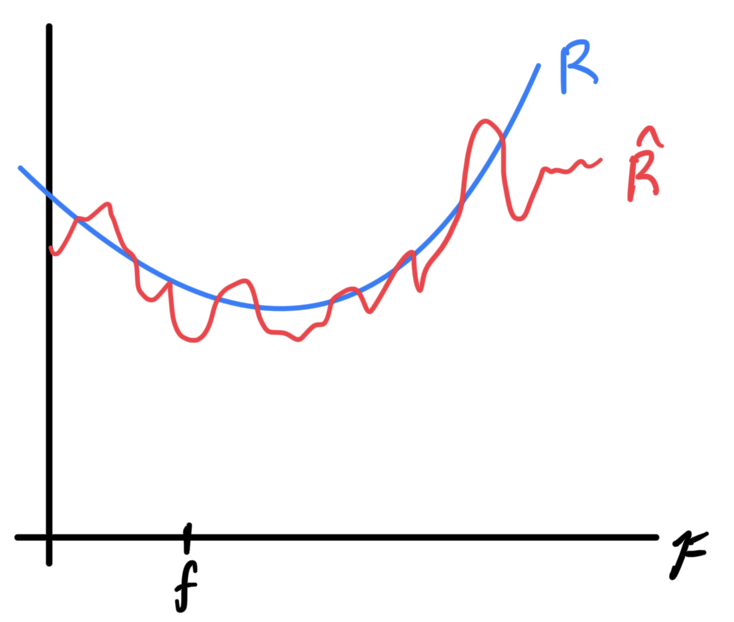
\includegraphics[scale=0.4]{img/True_vs_Empirical_Risk.png}
      \caption{True risk of functions over $\mathcal{F}$ and its noisy empirical risk. We want to bound the maximum deviation of these two over the whole class.} 
      \label{fig:true_vs_empirical_risk}
    \end{figure}
    \begin{equation}
      \mathbb{P} \big( \sup_{f \in \mathcal{F}} | \hat{R} (f) - R(f) | \geq \epsilon \big)
    \end{equation}
    This bound will depend on how \textit{complex} the function class $\mathcal{F}$ is, and to measure this complexity, we introduce some definitions. 

    \begin{definition}[Rademacher Complexity]
      Given \textbf{Rademacher random variables} $\sigma_1, \ldots, \sigma_n$ with $\mathbb{P}(\sigma_i = 1) = \mathbb{P}(\sigma_i = -1) = \frac{1}{2}$, the \textbf{Rademacher complexity} of a function class $\mathcal{F}$ is defined 
      \begin{equation}
        \mathrm{Rad}_n (\mathcal{F}) = \mathbb{E} \bigg[ \sup_{f \in \mathcal{F}} \bigg| \frac{1}{n} \sum_{i=1}^n \sigma_i f(Z_i) \bigg| \bigg]
      \end{equation}
      where the expectation is across the random $\sigma_i$'s and the $Z_i$'s, which are independent. 
    \end{definition}

    To get some intuition of what this is, let's consider a function class of a single function $f$. Then, the sup disappears and the term inside the absolute value sign becomes a $0$-mean random variable. Now if we have a very complex function class $\mathcal{F}$ with a lot of ``wiggly'' functions, then this value should be large. In this case, imagine a game where you pick generate some random variables $\sigma_i$ and the $Z_i$. Then, I pick a function that maximizes this value. How can I do that? If I can find a function $f$ that matches the sign of the $\sigma_i$'s ($+1$ or $-1$) at each of the values of $Z_i$, then this would be maximized. Therefore, if I have a sufficiently complex class, then I can pick a function that tracks your $\sigma_i$'s. Another way of looking at it is given noise variables $\sigma$ and $Z$, we're looking at the correlation between $\sigma$ and $f(Z)$. If we can maximize this correlation, then this is a complex class. 

    Now this is the most natural way of defining the complexity of the class, and in some cases it can be explicitly computed. However, in most cases it cannot be, but it can be bounded be something that is computable, like the VC dimension. 

    \begin{lemma}[Bigger Class, Bigger Complexity]
      If $\mathcal{F} \subset \mathcal{G}$, then $\mathrm{Rad}_n (\mathcal{F}) \leq \mathrm{Rad}_n (\mathcal{G})$.
    \end{lemma}

    \begin{lemma}[Convex Hull]
      If $\mathcal{F}$ is a convex set, then $\mathrm{Rad}_n (\mathcal{F}) = \mathrm{Rad}_n (\mathrm{conv}(\mathcal{F}))$, where $\mathrm{conv}(\mathcal{F})$ is the convex hull of $\mathcal{F}$.
    \end{lemma}

    This lemma is quite useful since if we have a certain finite set of functions, then their convex hull can encompass quite a bit, and we can also easily compute that convex hull's Rademacher complexity. Since the extremes haven't changed, the complexity doesn't change, and this might suggest that the Rademacher complexity is a good measure. 

    \begin{lemma}[Change of Complexity with Lipschitz Functions]
      Consider a $L$-Lipschitz function $g$  with $g(0) = 0$ and consider the class $\mathcal{F}$, then we can bound the class of functions $g \circ \mathcal{F} = \{ g \circ f \mid f \in \mathcal{F} \}$. 
      \begin{equation}
        \mathrm{Rad}_n (g \circ \mathcal{F}) \leq 2 L \mathrm{Rad}_n (\mathcal{F})
      \end{equation}
      This constant multiplicative bound is also useful. 
    \end{lemma}

    \begin{definition}[Projection of Function Class onto Points]
      Given a binary function class $\mathcal{F}$ with functions $f: \mathcal{X} \rightarrow \{0, 1\}$, let us denote the projection of $\mathcal{F}$ onto a set of points $z_1, \ldots, z_n \in \mathcal{X}$ to be 
      \begin{equation}
        \mathcal{F}_z = \mathcal{F}_{z_1, \ldots, z_n} = \{ (f(z_1), \ldots, f(z_n)) \mid f \in \mathcal{F} \}
      \end{equation}
      This projection determines the set of all possible binary labels that can be perfectly classified by some function $f$. 
    \end{definition}

    \begin{definition}[Shattering Number]
      The \textbf{shattering number} of $\mathcal{F}$ is defined 
      \begin{equation}
        s_n (\mathcal{F}) = s(\mathcal{F}, n) = \sup_{z_1, \ldots, z_n} |\mathcal{F}_{z_1, \ldots, z_n}|
      \end{equation}
      The highest number that this can be is $2^n$, since this is the number of possible binary vectors of length $n$. Given a set of $n$ points $z_1, \ldots, z_n$, we say that the function class $\mathcal{F}$ \textbf{shatters} this set if $\mathcal{F}_{z_1, \ldots, z_n} = |2^n|$. That is, for every one of the $2^n$ labels on the points, there exists a function that can perfectly classify them. 
    \end{definition}

    \begin{example}[Binary Functions]
      Consider the function class $\mathcal{F}$ of all binary functions of the form 
      \begin{equation}
        f(x) = \begin{cases} 1 & \text{ if } x > t \\
          0 & \text{ if } x \leq t \end{cases} 
      \end{equation}
      Then, the projection of $\mathcal{F}$ onto some $n = 3$ points is the set 
      \begin{equation}
        \{ (0, 0, 0), (0, 0, 1), (0, 1, 1), (1, 1, 1) \}
      \end{equation}
      and this is true no matter how I pick the $z_1, z_2, z_3$, and so the Shattering number is $s_n (\mathcal{F}) = 4$. 
    \end{example}

    \begin{definition}[VC Dimension]
      We know that the shattering number is bounded above by $2^n$. For $n = 1$, it is reasonable that it achieves this bound, but as $n$ grows, the Shattering number may die off. The point at which it dies off is the VC dimension. 
      \begin{figure}[H]
        \centering 
        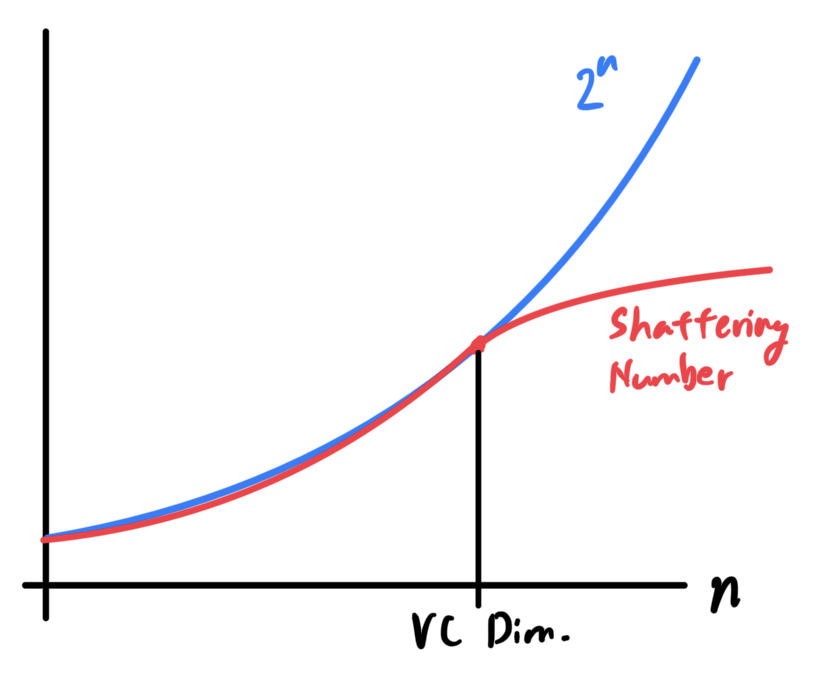
\includegraphics[scale=0.4]{img/Sawyer_lemma.png}
        \caption{The Shattering number of $\mathcal{F}$ will grow exponentially until it reaches the VC dimension, at which point it will grow polynomially.} 
        \label{fig:sawyer_lemma}
      \end{figure}
      That is, it is the largest $n$ number of points that can be shattered by the function class without misclassification. 
      \begin{equation}
        n^{\mathrm{VC}} \coloneqq \sup_n \{ s_n (\mathcal{F}) = 2^n \}
      \end{equation}
    \end{definition}

    It turns out that there are very interesting properties about the VC dimension. One such fact is Sawyer's lemma, which states that if the VC dimension is finite, then the rate of growth of the shattering number suddenly changes from exponential $2^n$ to polynomial $n^{\mathrm{VC}}$, and this is what makes a lot of machine learning work. 

    \begin{definition}[Subgaussian Random Variables]
      A random variable $X$ is \textbf{subgasussian} if 
      \begin{equation}
        \mathbb{E}[e^{\lambda X}] \leq e^{\frac{\lambda^2 \sigma^2}{2}}
      \end{equation}
      Gaussians and bounded random variables are subgaussian.
    \end{definition}

    \begin{lemma}[Bound on Subgaussian Random Variables]
      Given a set of iid subgaussian random variables $X_1, \ldots, X_n$ 
      \begin{equation}
        \mathbb{E}\big[ \max_{1 \leq i \leq d} X_i \big] \leq \sigma \sqrt{2 \log d}
      \end{equation}
    \end{lemma}

    \begin{theorem}[Bound of Rademacher Complexity with Shattering Number]
      The Rademacher complexity of a binary function class $\mathcal{F}$ is bounded by 
      \begin{equation}
        \mathrm{Rad}_n (\mathcal{F}) \leq \sqrt{\frac{2 \log s_n (\mathcal{F})}{n}}
      \end{equation}
    \end{theorem}
    \begin{proof}
      Given the projection $\mathcal{F}_{z_1, \ldots, z_n}$, we can use the law of iterated expectations on the Rademacher complexity. 
      \begin{align}
        \mathrm{Rad}_n (\mathcal{F}) & = \mathbb{E} \bigg[ \sup_{f \in \mathcal{F}} \bigg| \frac{1}{n} \sum_{i=1}^n \sigma_i f(Z_i) \bigg| \bigg] \\
                                     & = \mathbb{E}_{Z} \bigg[ \mathbb{E}_{\sigma} \bigg[ \sup_{f \in \mathcal{F}} \bigg| \frac{1}{n} \sum_{i=1}^n \sigma_i f(Z_i) \bigg| \; \mid \; Z_1, \ldots Z_n \bigg] \bigg] 
      \end{align}
      Note that in the inner expectation, since $f(Z_i)$ is now fixed, then are bounding a linear combination of a bunch of $\sigma_i$'s, which are subgaussian. Using the bound above, we can reduce it to 
      \begin{equation}
        \mathbb{E}_{Z} \bigg[ \sqrt{\frac{2 \log |F_{z_1, \ldots, z_n}|}{n}}\bigg] \leq \sqrt{\frac{2 \log s_n (\mathcal{F})}{n}} \leq \sqrt{\frac{2 d \log n}{n}} 
      \end{equation}
    \end{proof}

    However, this is not the best possible bound, and in cases such as K means clustering in high dimensions, this VC bound is terrible. Now we move onto the big VC theorem which now bounds the supremum of the difference between the empirical risk and the true risk. To prove this, we need a few tricks, the first being the symmetrization trick using ghost samples. 

    \begin{lemma}[Symmetrization Lemma]
      Given a set of random variables $Z_1, \ldots, Z_n$ and a function class $\mathcal{F}$, we can define ghost samples $Z_1^\prime, \ldots, Z_n^\prime$ that are iid copies of $Z_1, \ldots, Z_n$. Then, we can bound the Rademacher complexity of the function class $\mathcal{F}$ by 
      \begin{equation}
        \mathbb{P} \bigg( \sup_{f \in \mathcal{F}} | \hat{R} (f) - R(f) | \geq \epsilon \bigg) \leq 2 \mathbb{P} \bigg( \sup_{f \in \mathcal{F}} | \hat{R} (f) - \hat{R}^\prime (f) | \geq \epsilon / 2 \bigg)
      \end{equation}
      where $\hat{R}, \hat{R}^\prime$ is the empirical risk over the original and ghost samples, respectively. 
    \end{lemma}
    \begin{proof}
      Assume that we have a function $f$ that achieves this minimum. By the triangle inequality, 
      \begin{equation}
        | \hat{R} (f) - R(f)| > t \text{ and } | \hat{R}^\prime (f) - R(f)| < \frac{t}{2} \implies | \hat{R} (f) - \hat{R}^\prime (f) | > \frac{t}{2}
      \end{equation}
      We write this again as an indicator function. 
      \begin{equation}
        \mathbbm{1} (| \hat{R} (f) - R(f)| > t, | \hat{R}^\prime (f) - R(f)| < \frac{t}{2}) \implies \mathbbm{1} (| \hat{R} (f) - \hat{R}^\prime (f) | > \frac{t}{2})
      \end{equation}
      and since the samples and the ghost samples are independent, we can take the probability over the ghost samples to get 
      \begin{equation}
        \mathbbm{1} (| \hat{R} (f) - R(f)| > t) \, \mathbb{P}_{Z^\prime} (| \hat{R}^\prime (f) - R(f)| < \frac{t}{2}) \implies \mathbb{P}_{Z^\prime} (| \hat{R} (f) - \hat{R}^\prime (f) | > \frac{t}{2})
      \end{equation}
      and the rest of the proof can be found online. 
    \end{proof}

    The reason we want this is that it removes the $R(f)$, which is some unknown true mean that can be hard to deal with since it takes infinite values. It's easier to work with two empirical risks than deal with the true risk. 

    \begin{theorem}[VC Theorem/Inequality]
      Given a binary function class $\mathcal{F}$, we have
      \begin{equation}
        \mathbb{P} \bigg( \sup_{f \in \mathcal{F}} | \hat{R} (f) - R(f) | \geq \epsilon \bigg) \leq 2 S(\mathcal{F}, n) e^{-n \epsilon^2 / 8} \approx n^d e^{-n \epsilon^2 / 8}
      \end{equation}
      You can see that the exponential term is from Hoeffding but there is an extra cost of taking the supremum over the whole function class, which is the shattering number.
    \end{theorem}
    \begin{proof}
      Given $Z_1, \ldots, Z_n \sim \mathbb{P}$, we take a new set of random variables $Z_1^\prime, \ldots, Z_n^\prime$ that are iid copies of $Z_1, \ldots, Z_n$, called \textit{ghost samples}. 
    \end{proof}

    Therefore, for some classes of sets with finite VC dimension, the shattering term will grow polynomially in $n$ but the exponential term decays faster, which is what makes this work. That's why as $n$ grows, we can get a good bound on the supremum of this difference. 

    \begin{theorem}
      With probability $\geq 1 - \delta$, we have 
      \begin{equation}
        \sup_{f \in \mathcal{F}} | \hat{R} (f) - R(f) | \leq 2 \mathrm{Rad}_n (\mathcal{F}) + \sqrt{\frac{\log (2 / \delta)}{2 n}}
      \end{equation}
    \end{theorem}

  \subsection{Bias Variance Noise Decomposition} 

    Let's do some further analysis on this. When you take a supremum over a function class, it decomposes into 3 terms. 
    \begin{enumerate}
      \item One of which quantifies how big the function class is (more variance). 
      \item One of which quantifies the distance between the truth and the function class (bias).  
      \item One is the noise term, which is the irreducible error. 
    \end{enumerate}

    \begin{example}[Bias and Variance Tradeoff in Polynomial Regression]
      Let's motivate this by trying to fit a polynomial on some data. 
      \begin{figure}[H]
        \centering 
        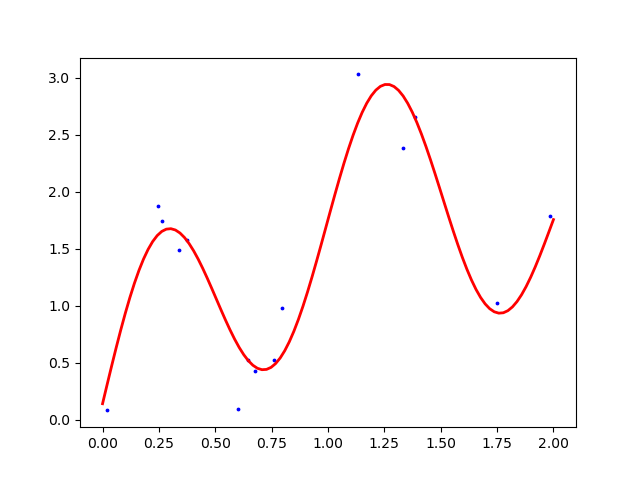
\includegraphics[scale=0.4]{img/True_data.png}
        \caption{A sample of $|\mathcal{D}| = 15$ data points are generated from the function $f(x) = \sin(2\pi x) + 2\cos (x - 1.5)$ with Gaussian noise $N(0, 0.3)$ on the interval $[0, 1]$. } 
        \label{fig:true_data}
      \end{figure}

      If we try to fit a polynomial function, how do we know which degree is best? Well the most simple thing is to just try all of them. To demonstrate this even further, I generated 10 different datasets  $\mathcal{D}$ of size $15$ taken from the same true distribution. The best fitted polynomials for each dataset is shown below. 

      \begin{figure}[H]
        \centering 
        \begin{subfigure}[b]{0.32\textwidth}
        \centering
          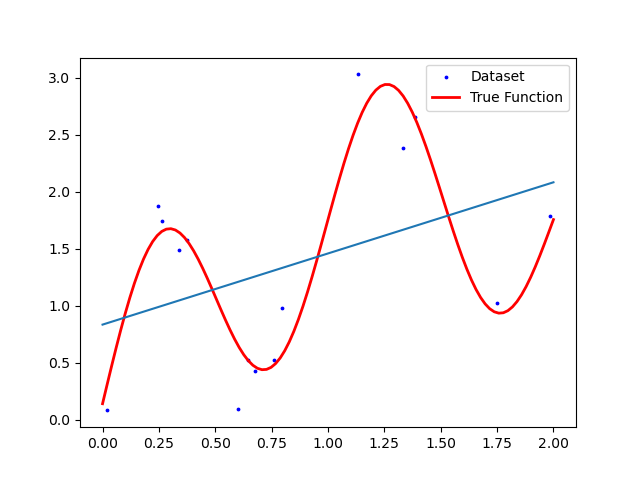
\includegraphics[width=\textwidth]{img/poly_1_fit.png}
          \caption{1st Degree}
          \label{fig:1d}
        \end{subfigure}
        \hfill 
        \begin{subfigure}[b]{0.32\textwidth}
        \centering
          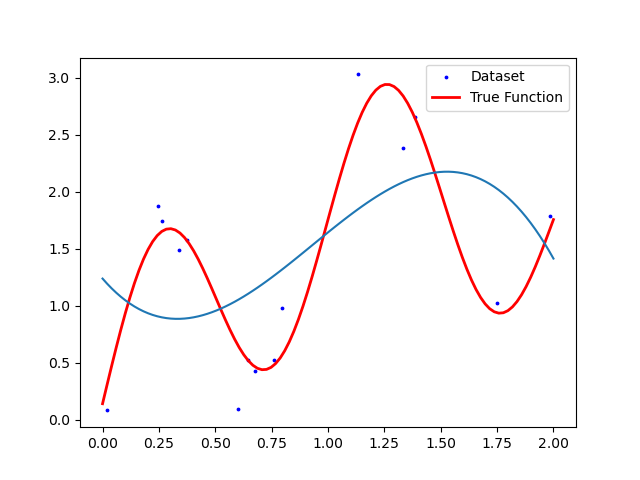
\includegraphics[width=\textwidth]{img/poly_3_fit.png}
          \caption{3rd Degree}
          \label{fig:3d}
        \end{subfigure}
        \hfill 
        \begin{subfigure}[b]{0.32\textwidth}
        \centering
          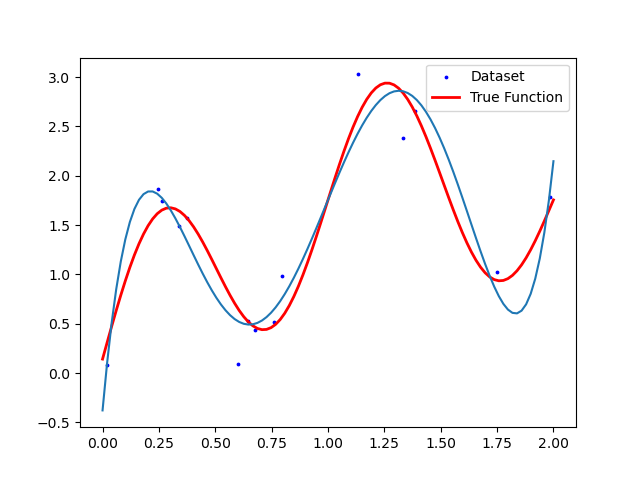
\includegraphics[width=\textwidth]{img/poly_5_fit.png}
          \caption{5th Degree}
          \label{fig:5e}
        \end{subfigure}

        \begin{subfigure}[b]{0.32\textwidth}
        \centering
          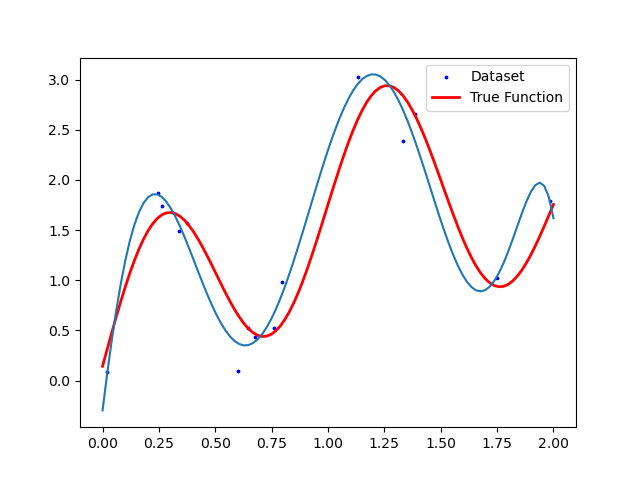
\includegraphics[width=\textwidth]{img/poly_7_fit.png}
          \caption{7th Degree}
          \label{fig:7d}
        \end{subfigure}
        \hfill 
        \begin{subfigure}[b]{0.32\textwidth}
        \centering
          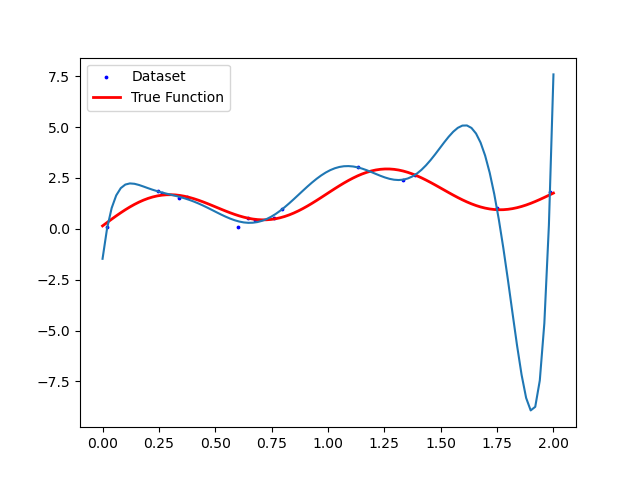
\includegraphics[width=\textwidth]{img/poly_9_fit.png}
          \caption{9th Degree}
          \label{fig:9d}
        \end{subfigure}
        \hfill 
        \begin{subfigure}[b]{0.32\textwidth}
        \centering
          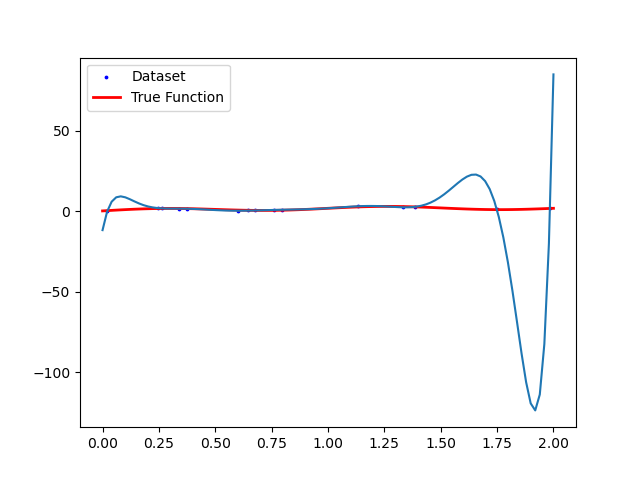
\includegraphics[width=\textwidth]{img/poly_11_fit.png}
          \caption{11th Degree}
          \label{fig:11e}
        \end{subfigure}

        \caption{Different model complexities (i.e. different polynomial degrees) lead to different fits of the data generated from the true distribution. The lower degree best fit polynomials don't have much variability in their best fits but have high bias, while the higher degree best fit polynomials have very high variability in their best fits but have low bias. The code used to generate this data is \href{code/polynomial_fitting.ipynb}{here}. }
        \label{fig:polynomial_fitting}
      \end{figure}

      We already know that the 5th degree approximation is most optimal, and the lower degree ones are \textbf{underfitting} the data, while the higher degree ones are \textbf{overfitting}. As mentioned before, we can describe the underfitting and overfitting phenomena through the bias variance decomposition. 

      \begin{enumerate}
        \item If we underfit the data, this means that our model is not robust and does not capture the patterns inherent in the data. It has a high bias since the set of function it encapsulates is not large enough to model $\mathbb{E}[Y\mid X]$. However, it has a low variance since if we were to take different samples of the dataset $\mathcal{D}$, the optimal parameters would not fluctuate. 

        \item What overfitting essentially means is that our model is too complex to the point where it starts to fit to the \textit{noise} of the data. This means that the variance is high, since different samples of the dataset $\mathcal{D}$ would cause huge fluctuations in the optimal trained parameters $\boldsymbol{\theta}$. However, the function set would be large, and thus it would be close to $\mathbb{E}[Y \mid X]$, leading to a low bias. 
      \end{enumerate}
    \end{example}
    
    \begin{example}[Polynomial Regression Continued]
      Another way to reduce the overfitting problem is if we have more training data to work with. That is, if we were to fit a 9th degree polynomial on a training set of not $N = 15$, but $N = 100$ data points, then we can see that this gives a much better fit. This makes sense because now the random variable $\mathcal{D}$, as a function of more random variables, has lower variance. Therefore, the lower variance in the dataset translates to lower variance in the optimal parameter. 

      \begin{figure}[H]
        \centering
        \begin{subfigure}[b]{0.48\textwidth}
        \centering
          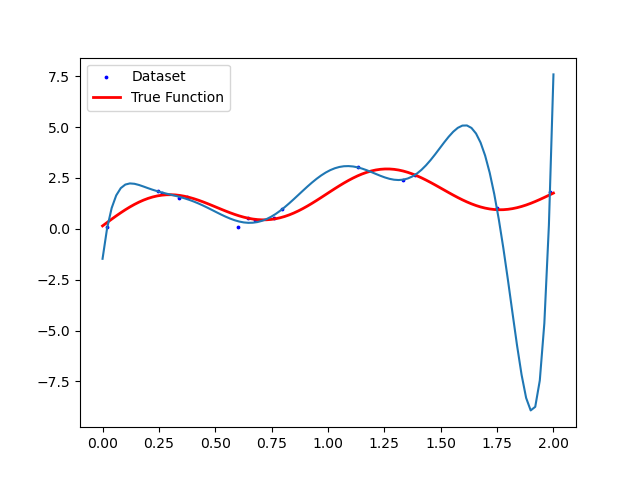
\includegraphics[width=\textwidth]{img/poly_9_fit.png}
          \caption{$M = 9, N = 15$}
          \label{fig:less_points}
        \end{subfigure}
        \hfill 
        \begin{subfigure}[b]{0.48\textwidth}
        \centering
          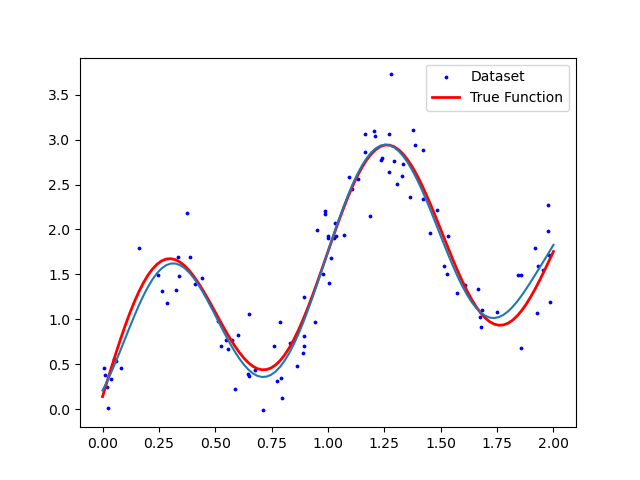
\includegraphics[width=\textwidth]{img/increased_data.png}
          \caption{$M = 9, N = 100$}
          \label{fig:more_points}
        \end{subfigure}
        \caption{Increasing the number of data points helps the overfitting problem. Now, we can afford to fit a 9th degree polynomial with reasonable accuracy.}
        \label{fig:reducing_overfitting_with_more_samples}
      \end{figure}
      
    \end{example}


  \subsection{Minimax Theory}

\section{Low Dimensional Linear Regression}

    In introductory courses, we start with linear predictors since it is easy to understand. We still start with linear predictors because in high-dimensional machine learning, even linear prediction can be hard as we will see. Low dimensional linear regression is what statisticians worked in back in the early days, where data was generally low dimensional.\footnote{Quoting Larry Wasserman, even 5 dimensions was considered high and 10 was considered massive. } Generally, we had $d < n$, but these days, we are in the regime where $d > n$. For example, in genetic data, you could have a sample of $n = 100$ people but each of them have genetic sequences at $d = 10^6$. When the dimensions become high, the original methods of linear regression tend to break down, which is why I separate low and high dimensional linear regression. The line tends to be fuzzy between these two regimes, but we will not worry about strictly defining that now. 

    In here, we start with \textbf{multiple linear regression}, which assumes that we have several covariates and one response. If we extend this to multiple responses (i.e. a response vector), this is called \textbf{multivariate linear regression}. The simple case for one response is called \textbf{simple linear regression}, and we will mention some nice formulas and intuition that come out from working with this. 

    \begin{definition}[Linear Regression Model]
      Given a dataset $\mathcal{D} = \{(x^{(i)}, y^{(i)})\}_{i=1}^n$, where $x^{(i)} \in \mathbb{R}^d$ with $x_1 = 1$ (which is what we do in practice to include an intercept term) and $y^{(i)} \in \mathbb{R}$, the multiple linear regression model is 
      \begin{equation}
        y = \beta^T x + \epsilon
      \end{equation}
      with the following assumptions: 
      \begin{enumerate}
        \item \textit{Weak exogeneity}: the covariates are observed without error.
        \item \textit{Linearity}: the mean of the variate is a linear combination of the parameters and the covariates.
        \item \textit{Gaussian errors}: the errors are Gaussian.\footnote{We can relax this assumption when we get into generalized linear models, and in most cases we assume some closed form of the error for computational convenience, like when computing the maximum likelihood.}
        \item \textit{Homoscedasticity}: the errors (the observations of $Y$) have constant variance. 
        \item \textit{Independence of errors}: The errors are uncorrelated.
        \item \textit{No multicollinearity}: more properly, the lack of perfect multicollinearity. Assume that the covariates aren't perfectly correlated.\footnote{This is the assumption that breaks down in high dimensional linear regression.} 
      \end{enumerate}
    \end{definition}

    In order to check multicollinearity, we compute the correlation matrix. 

    \begin{definition}[Correlation Matrix]
      The correlation matrix of random variables $X_1, \ldots, X_d$ is 
      \[\mathbf{C}_{ij} = \Corr(X_i, X_j) = \frac{\Cov(X_i, X_j)}{\sigma_{X_i} \sigma_{X_j}}\]
      given that $\sigma_{X_i} \sigma_{X_j} > 0$. Clearly, the diagonal entries are $1$, but if there are entries that are very close to $1$, then we have multicollinearity. 
    \end{definition}

    Assume that two variables are perfectly correlated. Then, there would be pairs of parameters that are indistinguishable if moved in a certain linear combination. This means that the variance of $\hat{\boldsymbol{\beta}}$ will be very ill conditioned, and you would get a huge standard error in some direction of the $\beta_i$'s. We can fix this by making sure that the data is not redundant and manually removing them, standardizing the variables, making a change of basis to remove the correlation, or just leaving the model as it is. 

    If these assumptions don't hold, 
    \begin{enumerate}
      \item \textit{Weak exogeneity}: the sensitivity of the model can be tested to the assumption of weak exogeneity by doing bootstrap sampling for the covariates and seeing how the sampling affects the parameter estimates.
      Covariates measured with error used to be a difficult problem to solve, as they required errors-in-variables models, which have very complicated likelihoods. In addition, there is no universal fitting library to deal with these. But nowadays, with the availability of Markov Chain Monte Carlo (MCMC) estimation through probabilistic programming languages, it is a lot easier to deal with these using Bayesian hierarchical models (or multilevel models, or Bayesian graphical models---these have many names).

      \item \textit{Linearity}: the linear regression model only assumes linearity in the parameters, not the covariates. Therefore you could build a regression using non-linear transformations of the covariates, for instance,
      \begin{equation}
        Y = X_1 \beta_1 + X_1^2 \beta_2 + \log(X_1) \beta_3
      \end{equation}
      If you need to further relax the assumption, you are better off using non-linear modelling. 

      \item \textit{Constant variance}: the simplest fix is to do a variance-stabilising transformation on the data. Assuming a constant coefficient of variation rather than a constant mean could also work. Some estimation libraries (such as the \verb+glm+ package in R) allow specifying the variance as a function of the mean.

      \item \textit{Independence of errors}: this is dangerous because in the financial world things are usually highly correlated in times of crisis. The most important thing is to understand how risky this assumption is for your setting. If necessary, add a correlation structure to your model, or do  a multivariate regression. Both of these require significant resources to estimate parameters, not only in terms of computational power but also in the amount of data required.

      \item \textit{No multicollinearity}: If the covariates are correlated, they can still be used in the regression, but numerical problems might occur depending on how the fitting algorithms invert the matrices involved. The t-tests that the regression produces can no longer be trusted. All the covariates must be included regardless of what their significance tests say.
      A big problem with multicollinearity, however, is over-fitting.
      Depending on how bad the situation is, the parameter values might have huge uncertainties around them, and if you fit the model using new data their values might change significantly.\footnote{I suggest reading this Wikipedia article on multicollinearity, as it contains useful information: \url{https://en.wikipedia.org/wiki/Multicollinearity}} Multicollinearity is a favourite topic of discussion for quant interviewers, and they usually have strong opinions about how it should be handled. The model's intended use will determine how sensitive it is to ignoring the error distribution. In many cases, fitting a line using least-squares estimation is equivalent to assuming errors have a normal distribution. If the real distribution has heavier tails, like the t-distribution, how risky will it make decisions based on your outputs? One way to address this is to use a technique like robust-regression. Another way is to think about the dynamics behind the problem and which distribution would be best suited to model them---as opposed to just fitting a curve through a set of points.
    \end{enumerate}

  \subsection{Ordinary Least Squares}

    If we use a squared loss function, this is called \textbf{ordinary least squares}. It is a well known fact that the true regressor that minimizes this loss is 
    \begin{equation}
      f^\ast (x) = \mathbb{E}[Y \mid X = x]
    \end{equation}
    which is the conditional expectation of $Y$ given $X$. This is the true regressor function, which is the best approximation of $Y$ over the $\sigma$-algebra generated by $X$. This may or may not be linear. 

    \begin{theorem}[Least Squares Solution For Linear Regression]
      Given the design matrix $\mathbf{X}$, we can present the linear model in vectorized form: 
      \begin{equation}
        \mathbf{Y} = \mathbf{X} \boldsymbol{\beta} + \boldsymbol{\epsilon}, \; \boldsymbol{\epsilon} \sim N(\mathbf{0}, \sigma^2 \mathbf{I})
      \end{equation}
      The solution that minimizes the squared loss is 
      \begin{align*}
        \boldsymbol{\beta} & = (\mathbf{X}^T \mathbf{X})^{-1} \mathbf{X}^T \mathbf{Y} \in \mathbb{R}^d \\
        \Var(\hat{\boldsymbol{\beta}}) & = \hat{\sigma}^2 (\mathbf{X}^T \mathbf{X})^{-1} \in \mathbb{R}^{d \times d}
      \end{align*}
    \end{theorem}
    \begin{proof}
      The errors can be written as $\boldsymbol{\epsilon} = \mathbf{Y} - \mathbf{X} \boldsymbol{\beta}$, and you have the following total sum of squared errors: 

      \[S(\boldsymbol{\beta}) = \boldsymbol{\epsilon}^T \boldsymbol{\epsilon} = (\mathbf{Y} - \mathbf{X} \boldsymbol{\beta})^T (\mathbf{Y} - \mathbf{X} \boldsymbol{\beta})\]

      We want to find the value of $\boldsymbol{\beta}$ that minimizes the sum of squared errors. In order to do this, remember the following matrix derivative rules when differentiating with respect to vector $\mathbf{x}$. 
      \begin{enumerate}
        \item $\mathbf{x}^T \mathbf{A} \mapsto \mathbf{A}$
        \item $\mathbf{x}^T \mathbf{A} \mathbf{x} \mapsto 2 \mathbf{A} \mathbf{x}$
      \end{enumerate}
      Now this should be easy. 
      \begin{align*}
          S(\boldsymbol{\beta}) & = \mathbf{Y}^T \mathbf{Y} - \boldsymbol{\beta}^T \mathbf{X}^T \mathbf{Y} - \mathbf{Y}^T \mathbf{X} \boldsymbol{\beta} + \boldsymbol{\beta}^T \mathbf{X}^T \mathbf{X} \boldsymbol{\beta} \\
          & = \mathbf{Y}^T \mathbf{Y} - 2 \mathbf{Y}^T \mathbf{X} \boldsymbol{\beta} + \boldsymbol{\beta}^T \mathbf{X}^T \mathbf{X} \boldsymbol{\beta} \\
          \frac{\partial}{\partial \boldsymbol{\beta}} S(\boldsymbol{\beta}) & = - 2 \mathbf{X}^T \mathbf{Y} + 2 \mathbf{X}^T \mathbf{X} \boldsymbol{\beta}
      \end{align*}
      and setting it to $\mathbf{0}$ gives 
      \[2 \mathbf{X}^T \mathbf{X} \boldsymbol{\beta} - 2 \mathbf{X}^T \mathbf{Y} = 0 \implies \mathbf{X}^T \mathbf{X} \boldsymbol{\beta} = \mathbf{X}^T \mathbf{Y}\]
      and the variance of $\boldsymbol{\beta}$, by using the fact that $\Var[\mathbf{A} \mathbf{X}] = \mathbf{A} \Var[X] \mathbf{A}^T$, is
      \[\Var(\hat{\boldsymbol{\beta}}) =
       (\mathbf{X}^{\prime} \mathbf{X})^{-1} \mathbf{X}^{\prime}
       \;\sigma^2 \mathbf{I} \; \mathbf{X}  (\mathbf{X}^{\prime} \mathbf{X})^{-1}
      = \sigma^2 (\mathbf{X}^{\prime} \mathbf{X})^{-1} (\mathbf{X}^{\prime}
       \mathbf{X})  (\mathbf{X}^{\prime} \mathbf{X})^{-1}
      = \sigma^2  (\mathbf{X}^{\prime} \mathbf{X})^{-1}\]
      But we don't know the true $\sigma^2$, so we estimate it with $\hat{\sigma}^2$ by taking the variance of the residuals. Therefore, we have 
      \begin{align*}
          \boldsymbol{\beta} & = (\mathbf{X}^T \mathbf{X})^{-1} \mathbf{X}^T \mathbf{Y} \in \mathbb{R}^d \\
          \Var(\hat{\boldsymbol{\beta}}) & = \hat{\sigma}^2 (\mathbf{X}^T \mathbf{X})^{-1} \in \mathbb{R}^{d \times d}
      \end{align*}
    \end{proof}

    \begin{example}[Copying Data]
      What happens if you copy your data in OLS? In this case, our MLE estimate becomes 
      \begin{align*}
          \left(\begin{pmatrix}X \\ X \end{pmatrix}^T \begin{pmatrix} X \\ X \end{pmatrix} \right )^{-1} & \begin{pmatrix} X \\ X  \end{pmatrix}^T \begin{pmatrix} Y \\ Y  \end{pmatrix}  =\\
      & = (X^T X + X^T X)^{-1} (X^T Y + X^T Y ) = (2 X^T X)^{-1} 2 X^T Y = \hat{\beta}
      \end{align*}
      and our estimate is unaffected. However, the variance shrinks by a factor of $2$ to 
      \begin{equation}
        \frac{\sigma^2}{2} (\mathbf{X}^T \mathbf{X})^{-1}
      \end{equation}
      A consequence of that is that confidence intervals will shrink with a factor of $1/\sqrt{2}$. The reason is that we have calculated as if we still had iid data, which is untrue. The pair of doubled values are obviously dependent and have a correlation of $1$. 
    \end{example}

    Another way to solve the solution is through likelihood estimation. 

    \begin{theorem}[Maximum Likelihood Estimation of Linear Regression]
      Given a dataset $\mathcal{D} = \{(x^{(i)}, y^{(i)})\}_{i=1}^N$, our likelihood is 
      \[L(\theta ; \mathcal{D}) = \prod_{i=1}^N p(y^{(i)} \mid x^{(i)}; \theta) = \prod_{i=1}^N \frac{1}{\sqrt{2 \pi \sigma^2}} \exp \bigg( -\frac{(y^{(i)} - \theta^T x^{(i)})^2}{2 \sigma^2} \bigg)\]
      We can take its negative log, remove additive constants, and scale accordingly to get 
      \begin{align*}
          \ell (\theta) & = -\frac{N}{2} \ln{\sigma^2} - \frac{N}{2} \ln(2 \pi) + \frac{1}{2 \sigma^2} \sum_{i=1}^N \big(y^{(i)} - \boldsymbol{\theta}^T \mathbf{x}^{(i)} \big)^2 \\
          & =\frac{1}{2} \sum_{i=1}^N \big(y^{(i)} - \boldsymbol{\theta}^T \mathbf{x}^{(i)} \big)^2 
      \end{align*}
      which then corresponds to minimizing the sum of squares error function. 
    \end{theorem}

    \begin{theorem}[Gradient Descent for Linear Regression]
      Taking the gradient of this log likelihood w.r.t. $\theta$ gives 
      \[\nabla_\theta \ell (\theta) = \sum_{i=1}^N ( y^{(i)} - \theta^T x^{(i)}) x^{(i)} \]
      and running gradient descent over a minibatch $M \subset \mathcal{D}$ gives 
      \begin{align*}
          \theta & = \theta - \eta \nabla_\theta \ell (\theta) \\
          & = \theta - \eta \sum_{(x, y) \in M} (y - \theta^T x) x
      \end{align*}
      This is guaranteed to converge since $\ell(\theta)$, as the sum of convex functions, is also convex. 

      Note that since we can solve this in closed form, by setting the gradient to $0$, we have 
      \[0 = \sum_{n=1}^N y^{(n)} \boldsymbol{\phi}(\mathbf{x}^{(n)})^T - \mathbf{w}^T \bigg( \sum_{n=1}^N \boldsymbol{\phi}(\mathbf{x}^{(n)}) \boldsymbol{\phi}(\mathbf{x}^{(n)})^T \bigg)\]
      which is equivalent to solving the least squares equation 
      \[\mathbf{w}_{ML} = ( \boldsymbol{\Phi}^T \boldsymbol{\Phi})^{-1} \boldsymbol{\Phi}^T \mathbf{Y}\]
      Note that if we write out the bias term out explicitly, we can see that it just accounts for the translation (difference) between the average of the outputs $\bar{y} = \frac{1}{N} \sum_{n=1}^N y_n$ and the average of the basis functions $\bar{\phi_j} = \frac{1}{N} \sum_{n=1}^N \phi_j (\mathbf{x}^{(n)})$. 
      \[w_0 = \bar{y} - \sum_{j=1}^{M-1} w_j \bar{\phi_j}\]
      We can also maximize the log likelihood w.r.t. $\sigma^2$, which gives the MLE 
      \[\sigma^2_{ML} = \frac{1}{N} \sum_{n=1}^N \big( y^{(n)} - \mathbf{w}^T_{ML} \boldsymbol{\phi}(\mathbf{x}^{(n)}) \big)^2\]
    \end{theorem}

    \begin{code}[MWE for OLS Linear Regression in scikit-learn]
      Here is a minimal working example of performing linear regression with scikit-learn. Note that the input data must be of shape $(n, d)$. 

      \noindent\begin{minipage}{.6\textwidth}
      \begin{lstlisting}[]{Code}
        import numpy as np 
        from sklearn.linear_model import LinearRegression 

        X = np.array([[1, 1], [1, 2], [2, 2], [2, 3]]) 
        y = np.dot(X, np.array([1, 2])) + 3 

        model = LinearRegression()  
        model.fit(X, y) 
        print(X) 
        print(y)
        print(model.score(X, y))  
        print(model.intercept_)
        print(model.coef_) 
        print(model.predict(np.array([[3, 5]])))
      \end{lstlisting}
      \end{minipage}
      \hfill
      \begin{minipage}{.39\textwidth}
      \begin{lstlisting}[]{Output}
        [[1 1]
         [1 2]
         [2 2]
         [2 3]]
        [ 6  8  9 11]
        1.0
        3.0000000000000018
        [1. 2.]
        [16.]
        .
        .
        .
        .
        .
      \end{lstlisting}
      \end{minipage}
    \end{code}

    \subsubsection{Bias Variance Decomposition} 

      We can use what we have learned to prove a very useful result for the mean squared loss. 

      \begin{theorem}[Pythagorean's Theorem]
        The expected square loss over the joint measure $\mathbb{P}_{X \times Y}$ can be decomposed as 
        \begin{equation}
          \mathbb{E}_{X \times Y} [( Y - h(X))^2] = \mathbb{E}_{X \times Y} [\big(Y - \mathbb{E}[Y \mid X]\big)^2] + \mathbb{E}_X [\big(\mathbb{E}[Y \mid X] - h(X) \big)^2]
        \end{equation}
        That is, the squared loss decomposes into the squared loss of $\mathbb{E}[Y \mid X]$ and $g(X)$, which is the intrinsic misspecification of the model, plus the squared difference of $Y$ with its best approximation $\mathbb{E}[Y\mid X]$, which is the intrinsic noise inherent in $Y$ beyond the $\sigma$-algebra of $X$. 
      \end{theorem}
      \begin{proof}
        We can write 
        \begin{align*}
          \mathbb{E}_{X \times Y} [L] & = \mathbb{E}_{X \times Y} \big[ \big(Y - g(X)\big)^2 \big] \\
          & = \mathbb{E}_{X \times Y}\big[ \big((Y - \mathbb{E}[Y \mid X]) + (\mathbb{E}[Y \mid X] - g(X)) \big)^2 \big] \\
          & = \mathbb{E}_{X \times Y} [\big(Y - \mathbb{E}[Y \mid X]\big)^2] + \mathbb{E}_{X \times Y} [\{Y - \mathbb{E} [Y \mid X]\} \, \{ \mathbb{E}[Y \mid X] - g(X) \}] \\
          & \;\;\;\;\;\;\;\;\;\;\;\;\;\;\; + \mathbb{E}_X [\big(\mathbb{E}[Y \mid X] - g(X) \big)^2] \\
          & = \mathbb{E}_{X \times Y} [\big(Y - \mathbb{E}[Y \mid X]\big)^2] + \mathbb{E}_X [\big(\mathbb{E}[Y \mid X] - g(X) \big)^2]
        \end{align*}

        where the middle term cancels out due to the tower property. 
      \end{proof}

      We also proved a second fact: Since $\mathbb{E}[\big(\mathbb{E}[Y \mid X] - g(X) \big)^2]$ is the misspecification of the model, we cannot change this (positive) constant, so $\mathbb{E}\big[ \big(Y - g(X)\big)^2 \big] \geq \mathbb{E}[(Y - \mathbb{E}[Y \mid X])^2]$, with equality achieved when we perfectly fit $g$ as $\mathbb{E}[Y \mid X]$ (i.e. the model is well-specified). Therefore, denoting $\mathcal{F}$ as the set of all $\sigma(X)$-measurable functions, then the minimum of the loss is attained when 
      \begin{equation}
        \argmin_{g \in \mathcal{F}} \mathbb{E}[L] = \argmin_{g \in \mathcal{F}} \mathbb{E} \big[ \big(Y - g(X)\big)^2 \big] = \mathbb{E}[Y \mid X]
      \end{equation}
      Even though this example is specific for the mean squared loss, this same decomposition, along with the bias variance decomposition, exists for other losses. It just happens so that the derivations are simple for the MSE, which is why this is introduced first. However, the derivations for other losses are much more messy, and sometimes may not hold rigorously. However, the general intuition that more complex models tend to overfit still hold true. 

      Now if we approximate $\mathbb{E}[Y \mid X]$ with our parameterized hypothesis $h_{\boldsymbol{\theta}}$, then from a Bayesian perspective the uncertainty in our model is expressed through a poseterior distribution over ${\boldsymbol{\theta}}$. A frequentist treatment, however, involves making a point estimate of ${\boldsymbol{\theta}}$ based on the dataset $\mathcal{D}$ and tries instead to interpret the uncertainty of this estimate through the following thought experiment: Suppose we had a large number of datasets each of size $N$ and each drawn independently from the joint distribution $X \times Y$. For any given dataset $\mathcal{D}$, we can run our learning algorithm and obtain our best fit function $h_{{\boldsymbol{\theta}}; \mathcal{D}}^\ast (\mathbf{x})$. Different datasets from the ensemble will give different functions and consequently different values of the squared loss. The performance of a particular learning algorithm is then assessed by taking the average over this ensemble of datasets, which we define $\mathbb{E}_\mathcal{D} [h_{{\boldsymbol{\theta}}; \mathcal{D}} (\mathbf{x})] = \mathbb{E}_{(X \times Y)^N} [h_{{\boldsymbol{\theta}}; \mathcal{D}} (\mathbf{x})]$. We are really taking an expectation over all datasets, meaning that the $N$ points in each $\mathcal{D}$ must be sampled from $(X \times Y)^N$. 

      Consider the term $\big(\mathbb{E}[Y \mid X] - h_{\boldsymbol{\theta}}(X) \big)^2$ above, which models the discrepancy in our optimized hypothesis and the best approximation. Now, over all datasets $\mathcal{D}$, there will be a function $h_{{\boldsymbol{\theta}}; \mathcal{D}}$, and averaged over all datasets $\mathcal{D}$ is $\mathbb{E}_\mathcal{D} [ h_{{\boldsymbol{\theta}}; \mathcal{D}}]$. So, the random variable below (of $\mathcal{D}$ and $X$) representing the stochastic difference between our optimized function $h_{{\boldsymbol{\theta}}; \mathcal{D}} (X)$ and our best approximation $\mathbb{E}[Y\mid X]$ can be decomposed into 

      \begin{align*}
        \big(\mathbb{E}[Y \mid X] - h_{{\boldsymbol{\theta}}:\mathcal{D}} (X) \big)^2 & =  \big[ \big( \mathbb{E}[Y \mid X] - \mathbb{E}_\mathcal{D} [h_{{\boldsymbol{\theta}}; \mathcal{D}} (X)] \big) + \big( \mathbb{E}_\mathcal{D} [h_{{\boldsymbol{\theta}}; \mathcal{D}} (X)] - h_{{\boldsymbol{\theta}}:\mathcal{D}} (X) \big) \big]^2 \\
        & = \big( \mathbb{E}[Y \mid X] - \mathbb{E}_\mathcal{D} [h_{{\boldsymbol{\theta}}; \mathcal{D}} (X)] \big)^2 + \big( \mathbb{E}_\mathcal{D} [h_{{\boldsymbol{\theta}}; \mathcal{D}} (X)] - h_{{\boldsymbol{\theta}}:\mathcal{D}} (X) \big)^2 \\
        & \;\;\;\;\;\;\;\; + 2 \big( \mathbb{E}[Y \mid X] - \mathbb{E}_\mathcal{D} [h_{{\boldsymbol{\theta}}; \mathcal{D}} (X)] \big) \big( \mathbb{E}_\mathcal{D} [h_{{\boldsymbol{\theta}}; \mathcal{D}} (X)] - h_{{\boldsymbol{\theta}}:\mathcal{D}} (X) \big) \\
        & = \big( \mathbb{E}[Y \mid X] - \mathbb{E}_\mathcal{D} [h_{{\boldsymbol{\theta}}; \mathcal{D}} (X)] \big)^2 + \big( \mathbb{E}_\mathcal{D} [h_{{\boldsymbol{\theta}}; \mathcal{D}} (X)] - h_{{\boldsymbol{\theta}}:\mathcal{D}} (X) \big)^2 
      \end{align*}

      Averaging over all datasets $\mathcal{D}$ causes the middle term to vanish and gives us the expected squared difference between the two random variables, now of $X$. 

      \begin{theorem}[Bias Variance Decomposition]
        Therefore, we can write out the expected square difference between $h_{\boldsymbol{\theta}}$ and $\mathbb{E}[Y\mid X]$ as the sum of two terms. 
        \begin{equation}
          \mathbb{E}_\mathcal{D} \big[ \big(\mathbb{E}[Y \mid X] - h_{\boldsymbol{\theta}}(X) \big)^2 \big] = \underbrace{\big( \mathbb{E}[Y \mid X] - \mathbb{E}_\mathcal{D} [h_{{\boldsymbol{\theta}}; \mathcal{D}} (X)] \big)^2}_{\text{(bias)}^2} + \underbrace{ \mathbb{E}_\mathcal{D} \big[ \big( \mathbb{E}_\mathcal{D} [h_{{\boldsymbol{\theta}}; \mathcal{D}} (X)] - h_{\boldsymbol{\theta}; \mathcal{D}}(X) \big)^2 \big]}_{\text{variance}}
        \end{equation}
        Let us observe what these terms mean: 
        \begin{enumerate}
          \item The \textbf{bias} $\mathbb{E}[Y \mid X] - \mathbb{E}_\mathcal{D} [h_{{\boldsymbol{\theta}}; \mathcal{D}} (X)]$ is a random variable of $X$ that measures the difference in how the average prediction of our hypothesis function $\mathbb{E}_\mathcal{D} [h_{{\boldsymbol{\theta}}; \mathcal{D}} (X)]$ differs from the actual prediction $\mathbb{E}[Y \mid X]$. 

          \item The \textbf{variance} $\mathbb{E}_\mathcal{D} \big[ \big( \mathbb{E}_\mathcal{D} [h_{{\boldsymbol{\theta}}; \mathcal{D}} (X)] - h_{{\boldsymbol{\theta}}; \mathcal{D}} (X) \big)^2 \big]$ is a random variable of $X$ that measures the variability of each hypothesis function $h_{\boldsymbol{\theta}}(X)$ about its mean over the ensemble $\mathbb{E}_\mathcal{D} [h_{{\boldsymbol{\theta}}; \mathcal{D}} (X)]$. 
        \end{enumerate}
      \end{theorem}

      Therefore, we can substitute this back into our Pythagoras decomposition, where we must now take the expected bias and the expected variance. Therefore, we get 
      \begin{equation}
        \text{Expected Loss} = (\text{Expected Bias})^2 + \text{Expected Variance} + \text{Noise}
      \end{equation}
      where 
      \begin{align*}
        (\text{Bias})^2 & = \mathbb{E}_X \big[ \big( \mathbb{E}[Y \mid X] - \mathbb{E}_\mathcal{D} [h_{{\boldsymbol{\theta}}; \mathcal{D}} (X)] \big)^2 \big] \\
        \text{Variance} & = \mathbb{E}_X \big[ \mathbb{E}_\mathcal{D} \big[ \big( \mathbb{E}_\mathcal{D} [h_{{\boldsymbol{\theta}}; \mathcal{D}} (X)] - h_{\boldsymbol{\theta}; \mathcal{D}}(X) \big)^2 \big] \big] \\
        \text{Noise} & = \mathbb{E}_{X \times Y}[\big(Y - \mathbb{E}[Y \mid X]\big)^2]
      \end{align*}

    \subsubsection{Convergence Bounds} 

      Let's get a deeper understanding on linear regression by examining the convergence of the empirical risk minimizer to the true risk minimizer. We can develop a naive bound using basic concentration of measure. 

      \begin{theorem}[Exponential Bound]
        Let $\mathcal{P}$ be the set of all distributions for $X \times Y$ supported on a compact set. There exists constants $c_1, c_2$ s.t. that the following is true. For any $\epsilon > 0$, 
        \begin{equation}
          \sup_{\mathbb{P} \in \mathcal{P}} \mathbb{P}^n \big( r(\hat{\beta}_n) > r (\beta_\ast (\mathbb{P}) + 2 \epsilon )\big) \leq c_1 e^{-n c_2 \epsilon^2}
        \end{equation}
        Hence 
        \begin{equation}
          r(\hat{\beta}_n ) - r(\beta_\ast) = O_{\mathbb{P}} \bigg( \sqrt{\frac{1}{n}} \bigg)
        \end{equation}
      \end{theorem} 
      \begin{proof}
        
      \end{proof}

      However, this is not a very tight bound, and we can do better. Though the proof is very long and will be omitted. 

      \begin{theorem}[Gyorfi, Kohler, Krzyzak, Walk, 2002 \cite{gyorfi2002distribution}] 
        Let $\sigma^2 = \sup_x \Var [Y \mid X = x] < \infty$. Assume that all random variables are bounded by $L < \infty$. Then 
        \begin{equation}
          \mathbb{E} \int |\hat{\beta}^T x - m(x) |^2 \, d\mathbb{P}(x) \leq 8 \inf_{\beta} \int |\beta^T x - m(x) |^2 \,d \mathbb{P}(x) + \frac{C d (\log(n) + 1)}{n}
        \end{equation}
      \end{theorem}

      You can see that the bound contains a term of the form 
      \begin{equation}
        \frac{d \log(n)}{n}
      \end{equation}
      and under the low dimensional case, $d$ is small and bound is good. However, as $d$ becomes large, then we don't have as good of theoretical guarantees. 

      \begin{theorem}[Central Limit Theorem of OLS]
        We have 
        \begin{equation}
          \sqrt{n} (\hat{\beta} - \beta) \xrightarrow{d} N(0, \Gamma) 
        \end{equation}
        where 
        \begin{equation}
          \Gamma = \Sigma^{-1} \mathbb{E} \big[ (Y - X^T \beta)^2 X X^T \big] \Sigma^{-1}
        \end{equation}
        The covariance matrix $\Gamma$ can be consistently estimated by 
        \begin{equation}
          \hat{\Gamma} = \hat{\Sigma}^{-1} \hat{M} \hat{\Sigma}^{-1}
        \end{equation}
        where 
        \begin{equation}
          \hat{M} (j, k) = \frac{1}{n} \sum_{i=1}^n X_i (j) X_i (k) \hat{\epsilon}_i^2
        \end{equation}
        and $\hat{\epsilon}_i = Y_i - \hat{\beta}^T X_i$.
      \end{theorem}

  \subsection{Simple Linear Regression}

    The simple linear regression is the special case of the linear regression with only one covariate.\footnote{I've included a separate section on this since this was especially important for quant interviews.}
    \begin{equation}
      y = \alpha + x \beta
    \end{equation}
    which is just a straight line fit. Interviewers like this model for its aesthetically pleasing theoretical properties. A few of them are described here, beginning with parameter estimation. For $n$ pairs of $(x_i, y_i)$, 
    \begin{equation}
      y_i = \alpha + \beta x_i + \epsilon_i
    \end{equation}
    To minimize the sum of squared errors 
    \begin{equation}
      \sum_{i} \epsilon_i^2 = \sum_{i} (y_i - \alpha - \beta x_i)^2
    \end{equation}
    Taking the partial derivatives w.r.t. $\alpha$ and $\beta$ and setting them equal to $0$ gives 
    \begin{align*}
      &\sum_i (y_i - \hat{\alpha} - \hat{\beta} x_i) = 0 \\
      &\sum_i (y_i - \hat{\alpha} - \hat{\beta} x_i) x_i = 0
    \end{align*}
    From just the first equation, we can write 
    \begin{equation}
      n \bar{y} = n \hat{\alpha} + n \hat{\beta} \bar{x} \implies y = \hat{\alpha} + \hat{\beta} \bar{x} \implies \hat{\alpha}  = \bar{y} - \hat{\beta} \bar{x} 
    \end{equation}
    The second equation gives 
    \begin{equation}
      \sum_{i} x_i y_i = \hat{\alpha} n \bar{x} + \hat{\beta} \sum_{i} x_i^2
    \end{equation}
    and substituting what we derived gives 
    \begin{align*}
      \sum_{i} x_i y_i & = (\bar{y} - \hat{\beta} \bar{x}) n \bar{x} + \hat{\beta} \sum_i x_i^2 \\
      & = n \bar{x} \bar{y} + \hat{\beta} \bigg( \Big(\sum_i x_i^2 \Big) - n \bar{x}^2 \bigg)
    \end{align*}
    and so we have 
    \begin{equation}
      \hat{\beta} = \frac{ \big( \sum_i x_i y_i \big) - n \bar{x}\bar{y}}{\big( \sum x_i^2 \big) - n \bar{x}^2} = \frac{ \sum_i x_i y_i - \bar{x} y_i}{\sum x_i^2 - \bar{x} x_i} = \frac{ \sum_i (x_i - \bar{x}) y_i}{\sum_i (x_i - \bar{x}) x_i}
    \end{equation}
    Now we can use the identity
    \begin{align*}
      \sum_{i} (x_i - \bar{x}) (y_i - \bar{y}) & = \sum_i y_i (x_i - \bar{x}) = \sum_i x_i (y_i - \bar{y}) 
    \end{align*}
    to substitute both the numerator and denominator of the equation to 
    \begin{align*}
      \hat{\beta} & = \frac{\sum_i (x_i - \bar{x}) (y_i - \bar{y})}{\sum_i (x_i - \bar{x})^2} = \frac{\mathrm{cov}(x, y)}{\mathrm{var}(x)} = \rho_{xy} \frac{s_y}{s_x}
    \end{align*}
    where $\rho_{xy}$ is the correlation between $x$ and $y$, and the variance and covariance represent the sample variance and covariance (indicated in lower case letters). Therefore, the correlation coefficient $\rho_{xy}$ is precisely equal to the slope of the best fit line when $x$ and $y$ have been standardized first, i.e. $s_x = s_y = 1$. 

    \begin{example}[Switching Variables]
      Say that we are fitting $Y$ onto $X$ in a simple regression setting with MLE $\beta_1$, and now we wish to fit $X$ onto $Y$. How will the MLE slope change? We can see that 
      \[\beta_1 = \rho \frac{s_y}{s_x} , \;\; \beta_2 = \rho \frac{s_x}{s_y}\]
      and so 
      \[\beta_2 = \rho^2 \frac{1}{\rho} \frac{s_x}{s_y} = \rho^2 \frac{1}{\beta_1} = \beta_1 \frac{\mathrm{var}(x)}{\mathrm{var}(y)}\]
      The reason for this is because regression lines don't necessarily correspond to one-to-one to a casual relationship. Rather, they relate more directly to a conditional probability or best prediction. 
    \end{example}

    The \textbf{coefficient of determination} $R^2$ is a measure tells you how well your line fits the data. When you have your $y_i$'s, their deviation around its mean is captured by the sample variance $s^2_y = \sum_i (y_i - \bar{y})^2$. When we fit our line, we want the deviation of $y_i$ around our predicted values $\hat{y}_i$, i.e. our sum of squared loss $\sum_i (y_i - \hat{y}_i)^2$, to be lower. Therefore, we can define 
    \[R^2 = 1 - \frac{\mathrm{MSE Loss}}{\mathrm{var}(y)} = 1 - \frac{\sum_i (y_i - \hat{y}_i)^2}{\sum_i (y_i - \bar{y})^2}\]
    In simple linear regression, we have 
    \[R^2 = \rho_{yx}^2\]
    An $R^2$ of $0$ means that the model does not improve prediction over the mean model and $1$ indicates perfect prediction. However, a drawback of $R^2$ is that it can increase if we add predictors to the regression model, leading to a possible overfitting. 

    \begin{theorem}
      The residual sum of squares (RSS) is equal to the a proportion of the variance of the $y_i$'s. 
      \begin{equation}
        \mathrm{RSS} = \sum (y_i - \hat{y}_i)^2 = (1 - \rho^2) \sum (y_i - \bar{y})^2 
      \end{equation}
    \end{theorem}

  \subsection{Weighted Least Squares}


  \subsection{Mean Absolute Error}


  \subsection{Significance Tests}

    This is not as emphasized in the machine learning literature, but it is useful to know from a statistical point of view.\footnote{This is also asked in quant interviews.}

    \subsubsection{T Test}

      Given some multilinear regression problem where we must estimate $\boldsymbol{\beta} \in \mathbb{R}^{D + 1}$ ($D$ coefficients and $1$ bias), we must determine whether there is actually a linear relationship between the $x$ and $y$ variables in our dataset $\mathcal{D}$. Say that we have a sample of $N$ points $\mathcal{D} = \{(x_n, y_n)\}_{n=1}^N$. Then, for each ensemble of datasets $\mathcal{D}$ that we sample from the distribution $(X \times Y)^N$, we will have some estimator $\boldsymbol{\beta}$ for each of them. This will create a sampling distribution of $\boldsymbol{\beta}$'s where we can construct our significance test on. 

      So what should our sampling distribution of $\hat{\boldsymbol{\beta}}$ be? It is clearly normal since it is just a transformation of the normally distributed $Y$: $\hat{\boldsymbol{\beta}} \sim N (\boldsymbol{\beta}, \sigma^2 (X^T X)^{-1})$. Therefore, only considering one element $\beta_i$ here, 
      \[\frac{\hat{\beta}_i - \beta_i}{\sigma \sqrt{ (X^T X)^{-1}_{ii}}} \sim N(0, 1)\]
      But the problem is that we don't know the true $\sigma^2$, and we are estimating it with $\hat{\sigma}^2$. If we knew the true $\sigma^2$ then this would be a normal, but because of this estimate, our normalizing factor is also random. It turns out that the residual sum of squares (RSS) for a multiple linear regression
      \[\sum_{i} (y_i - x_i^T \beta)^2 \]
      follows a $\chi^2_{n-d}$ distribution. Additionally from the $\chi^2$ distribution of RSS we have 
      \[\frac{(n - d) \hat{\sigma}^2}{\sigma^2} \sim \chi^2_{n-d}\]
      where we define $\hat{\sigma}^2 = \frac{\mathrm{RSS}}{n-d}$ which is an unbiased estimator for $\sigma^2$. Now there is a theorem that says that if you divide a $N(0, 1)$ distribution by a $\chi^2_k / k$ distribution (with $k$ degrees of freedom), then it gives you a $t$-distribution with the same degrees of freedom. Therefore, we divide 
      \[\frac{\frac{\hat{\beta}_i - \beta_i}{\sqrt{ (X^T X)^{-1}_{ii}}}}{\hat{\sigma}} = \frac{ \sigma \sim N(0, 1)}{\sigma \chi^2_{n-d} / (n-d)} = \frac{\sim N(0, 1)}{\chi^2_{n-d} / (n-d)} = t_{n-d}\]
      where the standard error of the distribution is 
      \[\mathrm{SE}(\hat{\beta}_i) = \sigma_{\hat{\beta}_i} = \sigma \sqrt{(X^T X)^{-1}_{ii}} \]

      In ordinary linear regression, we have the null hypothesis $h_0 : \beta_i = 0$ and the alternative $h_a : \beta_i \neq 0$ for a two sided test or $h_a : \beta_i > 0$ for a one sided test. Given a certain significance level, we compute the critical values of the $t$-distribution at that level and compare it with the test statistic 
      \[t = \frac{\hat{\beta} - 0}{\mathrm{SE}(\hat{\beta})}\]

      Now given our $\beta$, how do we find the standard error of it? Well this is just the variance of our estimator $\boldsymbol{\beta}$, which is $\hat{\sigma}^2 (\mathbf{X}^T \mathbf{X})^{-1}$, where $\hat{\sigma}^2$ is estimated by taking the variance of the residuals $\epsilon_i$. When there is a single variable, the model reduces to 
      \[y = \beta_0 + \beta_1 x + \epsilon\]
      and 
      \[\mathbf{X} = \left(
      \begin{array}{cc}
      1 & x_1 \\
      1 & x_2 \\
      \vdots & \vdots \\
      1 & x_n
      \end{array}
      \right), \qquad \boldsymbol{\beta} = \left(
      \begin{array}{c}
      \beta_0 \\ \beta_1 
      \end{array}
      \right)\]
      and so 
      \[(\mathbf{X}^{\prime} \mathbf{X})^{-1} = \frac{1}{n\sum x_i^2 - (\sum x_i)^2} 
      \left(
      \begin{array}{cc}
      \sum x_i^2 & -\sum x_i \\
      -\sum x_i  & n
      \end{array}
      \right)\]
      and substituting this in gives 
      \[\sqrt{\widehat{\textrm{Var}}(\hat{\beta_1})} = \sqrt{[\hat{\sigma}^2  (\mathbf{X}^{\prime} \mathbf{X})^{-1}]_{22}} = \sqrt{\frac{\hat{\sigma}^2}{\sum x_i^2 - (\sum x_i)^2}} = \sqrt{\frac{\hat{\sigma}^2}{\sum (x_i - \bar{x}_i)^2}}\]

      \begin{example}
      Given a dataset 
      \begin{verbatim}
      Hours Studied for Exam 20 16 20 18 17 16 15 17 15 16 15 17 16 17 14
      Grade on Exam 89 72 93 84 81 75 70 82 69 83 80 83 81 84 76
      \end{verbatim}
      The hypotheses are $h_0 : \beta = 0$ and $h_a : \beta \neq 0$, and the degrees of freedom for the $t$-test is $df = N - (D + 1) = 13$, where $N = 15$ is the number of datapoints and $D = 1$ is the number of coefficients (plus the 1 bias term). The critical values is $\pm 2.160$, which can be found by taking the inverse CDF of the $t$-distribution evaluated at $0.975$. 

      Now we calculate the $t$ score. We have our estimate $\beta_1 = 3.216, \beta_0 = 26.742$, and so we calculate 
      \begin{align*}
          \hat{\sigma}^2 & = \frac{1}{15} \sum_{i=1}^{15} \big( y_i - (3.216 x_i + 26.742) \big) = 13.426 \\
          \sum_{i} (x_i - \hat{x}_i)^2 & = 41.6 
      \end{align*}
      and therefore, we can compute 
      \[t = \frac{\beta_1}{\sqrt{\hat{\sigma}^2 /  \sum_{i} (x_i - \hat{x}_i)^2}} = \frac{3.216}{\sqrt{13.426/41.6}} = 5.661\]
      and therefore, this is way further than our critical value of $2.16$, meaning that we reject the null hypothesis. 
      \end{example}

      Note that when multicolinearity is present, then $\sum_{i} (x_i - \hat{x}_i)^2$ will be very small causing the denominator to blow up, and therefore you cannot place too much emphasis on the interpretation of these statistics. While it is hard to see for the single linear regression case, we know that some eigenvalue of $(\mathbf{X}^T \mathbf{X})^{-1}$ will blow up, causing the diagonal entries $(\mathbf{X}^T \mathbf{X})^{-1}_{ii}$ to be very small. When we calculate the standard error by dividing by this small value, the error blows up. 

      \begin{theorem}
      We can compute this $t$-statistic w.r.t. just the sample size $n$ and the correlation coefficient $\rho$ as such. 
      \[t = \frac{\hat{\beta} - 0}{\mathrm{SE}(\hat{\beta})}\]
      and the denominator is simply 
      \begin{align*}
        \mathrm{SE}(\hat{\beta}) = \sqrt{\frac{\frac{1}{n-1} \sum (y_i - \hat{y})^2}{\sum (x_i - \bar{x})^2}} \implies t = \frac{\hat{\beta} \sqrt{\sum (x_i - \bar{x})^2} \sqrt{n-1}}{\sqrt{\sum (y_i - \hat{y})^2}} & = \frac{\hat{\beta} \sqrt{\sum (x_i - \bar{x})^2} \sqrt{n-1}}{\sqrt{(1 - \rho^2)} \sqrt{\sum (y_i - \bar{y})^2}} \\ & = \frac{\rho}{\sqrt{1 - \rho^2}} \sqrt{n-1}
      \end{align*}
      where the residual sum of squares on the top can be substituted according to our theorem. Therefore 
      \begin{equation}
        t = \frac{\rho}{\sqrt{1 - \rho^2}} \sqrt{n-1}
      \end{equation}
      \end{theorem}

    \subsubsection{F Test}

      Given that you have $n$ data points that have been fit on a linear model, the $F$-statistic is based on the ratio of two variances. 

  \subsection{Bayesian Linear Regression} 

\section{High Dimensional Linear Regression}

    Now supposed that $d > n$, then the first problem is that we can no longer use least squares since $X^T X$ is no longer invertible and the same problem happens with maximum likelihood. This is known as the \textbf{high dimensional} or \textbf{large $p$, small $n$} problem. The most straightforward way is simply to reduce the covariates to a dimension smaller than $n$. This can be done with three ways. 
    \begin{enumerate}
      \item We perform PCA on the $X$ and use the first $k$ principal components where $k < n$. 
      \item We cluster the covariates based on their correlation. We can use one feature from each cluster or take the average of the covariates within each cluster. 
      \item We can screen the variables by choosing the $k$ features that have the largest correlation with $Y$. 
    \end{enumerate}
    Once this is done, we are back in the low dimensional regime and can use least squares. Essentially, this is a way to find a good subset of the covariates, which can be formalized by the following. Let $S$ be a subset of $[d]$ and let $X_S = (X_j \,:\, j \in S)$. If the size of $S$ is not too large, we can regress $Y$ on $X_S$ instead of $X$. 

    \begin{definition}[Best Subset Regression]
      Fix $k < d$ and let $\mathcal{S}_k$ denote all subsets of size $k$. For a given $S \in \mathcal{S}_k$, let $\beta_S$ be the best linear predictor for the subset $S$. We want to find the best subset $S$ that minimizes the loss 
      \begin{equation}
        \mathbb{E} [ (Y - \beta_S^T X_S)^2] 
      \end{equation}
      which is equivalent to finding 
      \begin{equation}
        \argmin_{\beta} \mathbb{E} [ (Y - \beta^T X)^2] \text{ subject to } ||\beta||_0 \leq k
      \end{equation}
      where $||\beta||_0$ is the number of non-zero entries in $\beta$. 
    \end{definition}

    There will be a bias variance tradeoff. As $k$ increases, the bias decreases but the variance increases. We can approximate the risk with the training error, but the minimization is over all subset of size $k$, and so this is NP-hard. Therefore, best subset regression is infeasible, but we can approximate best subset regression in two different ways. 
    \begin{enumerate}
      \item A greedy approximation leads to \textit{forward stepwise regression}. 
      \item A convex relaxation of the problem leads to the \textit{LASSO} regression. 
    \end{enumerate}
    It turns out that the theoretical guarantees and computational time for both are the same, but the Lasso is much more popular. It may be due to a cleaner form or that it's easier to study, but who knows. 

    A completely separate way is to use all the covariates, but instead of least squares, we shrink the coefficients towards $0$. This is called \textit{ridge regression} and is an example of a \textit{shrinkage model}. 

  \subsection{Ridge Regression} 

    Ridge regression is used both in the high dimensional case or when our function space is too large/complex, which leads to overfitting. In the overfitting case, we have seen that either decreasing our function space or getting more training data helps. Another popular way is to add a \textbf{regularizing term} to the error function in order to discourage the coefficients from reaching large values, effectively limiting the variance over $\mathcal{D}$. 

    \begin{definition}[Ridge Regression]
      In \textbf{ridge regression}, we minimize 
      \begin{equation}
        L(\beta) = ||Y - X \beta||^2 + \lambda ||\beta||^2 
      \end{equation}
      where we penalize according to the L2 norm of the coefficients. 
    \end{definition}

    \begin{figure}[H]
      \centering
      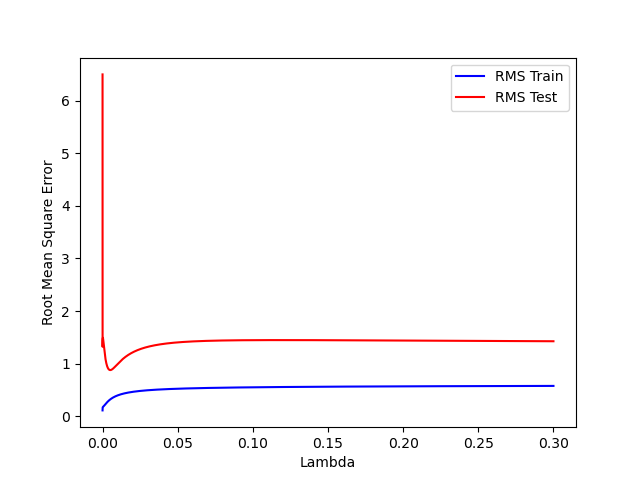
\includegraphics[scale=0.5]{img/Lambda_vs_RMS.png}
      \caption{Even with a slight increase in the regularization term $\lambda$, the RMS error on the testing set heavily decreases. }
      \label{fig:enter-label}
    \end{figure}

    \begin{theorem}[Least Squares Solution for Ridge Regression]
      The minimizer of the ridge loss is 
      \begin{equation}
        \hat{\beta} = (X^T X+ \lambda I)^{-1} X^T Y
      \end{equation}
    \end{theorem}
    \begin{proof}
      TBD
    \end{proof}

    \begin{theorem}[Bias Variance Decomposition of Ridge Regression]
      TBD 
    \end{theorem}

    From a computational point of view, we can see that by adding the $\lambda I$ term, it \textit{dampens} the matrix so that it does become invertible (or well conditioned), allowing us to find a solution. The higher the $\lambda$ term, the higher the damping effect. The next theorem compares the performance of the best ridge regression estimator to the best linear predictor. 

    \begin{theorem}[Hsu, Kakade, Zhang, 2014 \cite{hsu2014random}] 
      Suppose that $||X_i|| \leq r$ and let $\beta^T x$ be the best linear approximation to $m(x)$. Then, with probability at least $1 - 4 e^{-t}$, we have
      \begin{equation}
        r(\hat{\beta}) - r(\beta) \leq \bigg( 1 + O \bigg( \frac{1 + r^2 / \lambda}{n} \bigg) \bigg) \frac{\lambda ||\beta||^2}{2} + \frac{\sigma^2}{n} \frac{\Tr(\Sigma)}{2 \lambda}
      \end{equation}
    \end{theorem}

    We can see that the $\lambda$ term exists in the numerator on $\frac{\lambda ||\beta||^2}{2}$ and in the denominator on $\frac{\Tr(\Sigma)}{2 \lambda}$. This is the bias variance tradeoff. The first term is the bias term, which is the penalty for not being able to fit the data as well. The second term is the variance term, which is the penalty for having a more complex model. So our optimal $\lambda$ in the theoretical sense would be the one that minimizes the sum of these two terms. In practice, it's not this clean since we have unknown quantities in the formula, but just like how we did cross validation over the model complexity, we can also do cross validation over the $\lambda$. The decomposition above just gives you a theoretical feeling of how these things trade off. 

    \begin{code}[MWS of Ridge Regression in scikit-learn]
      \noindent\begin{minipage}{.6\textwidth}
      \begin{lstlisting}[]{Code}
        import numpy as np 
        from sklearn.linear_model import Ridge  

        X = np.random.randn(10, 5) 
        y = np.random.randn(10)
        # regularization parameter
        model = Ridge(alpha=1.0)  
        model.fit(X, y) 
        print(model.score(X, y))  
        print(model.intercept_)
        print(model.coef_) 
        print(model.predict(np.array([[1, 2, 3, 4, 5]]))) 
      \end{lstlisting}
      \end{minipage}
      \hfill
      \begin{minipage}{.39\textwidth}
      \begin{lstlisting}[]{Output}
        0.8605535024325397
        -0.28291076492665157
        [-0.10400521 -0.7587073  -0.05116735  1.16236649 -0.0401323 ]
        [2.39097184]
        .
        .
        .
        .
        .
        .
      \end{lstlisting}
      \end{minipage}
    \end{code}

    \begin{question}[To Do]
      Bayesian interpretation of ridge regression. 
    \end{question}

  \subsection{Forward Stepwise Regression} 

    Forward stepwise regression is a greedy algorithm that starts with an empty set of covariates and adds the covariate that most improves the fit. It avoids the NP-hardness of the best subset regression by adding covariates one by one. 

    \begin{definition}[Greedy Forward Stepwise Regression]
      Given your data $\mathcal{D}$, let's first standardize it to have mean $0$ and variance $1$.\footnote{This may or may not be a good idea, since the variance of each covariate can tell you a lot about the importance of the covariate.} You start off with a set $\mathcal{Q} = \{\}$ and choose the number of parameters $K$. 
      \begin{enumerate}
        \item With each covariate $X = (X_1, \ldots, X_n)$, we compute the correlation between it and the $Y$, which reduces to the inner product (since we standardized). 
        \begin{equation}
          \rho_j = \langle Y, X_{:, j} \rangle = \frac{1}{n} \sum_{i=1}^n Y_i X_{ji}
        \end{equation}

        \item Then, we take the covariate index that has the highest empirical correlation with $Y$, add it to $\mathcal{Q}$ and regress $Y$ only on this covariate. 
        \begin{equation}
          q_1 = \argmax_j \rho_j , \;\; \mathcal{Q} = \{q_1\}, \;\; \hat{\beta}_{q_1} = \argmin_{\beta} \frac{1}{n} ||Y - X_{:, q_1} \beta||^2 
        \end{equation}

        \item Then you repeat the process. You take the residual values $r = Y - X_{:, q_1} \hat{\beta}_{q_1} \in \mathbb{R}^n$ compute the correlation between $r$ and the remaining covariates, and pick our the maximum covariate index $q_2$. Then, you \textit{repeat the regression from start} with these two covariates 
        \begin{equation}
          q_2 = \argmax_j \langle r, X_{: ; j} \rangle , \;\; \mathcal{Q} = \{q_1, q_2\}, \;\; \hat{\beta}_{q_1, q_2} = \argmin_{\beta} \frac{1}{n} ||Y - X_{:,[q_1, q_2]} \beta||^2
        \end{equation}
        Note that you're not going to get the same coefficient for $\hat{\beta}_{q_1}$ as before since you're doing two variable regression. 

        \item You get out the residual values $r = Y - X_{:, [q_1, q_2]} \hat{\beta}_{q_1, q_2} \in \mathbb{R}^n$ and keep repeating this process until you have $K$ covariates in $\mathcal{Q}$. 
      \end{enumerate}
    \end{definition}

    Again, there is a bias variance tradeoff in choosing the number of covariates $K$, but through cross-validation, we can find the optimal $K$. It is also easy to add constraints, e.g. if we wanted to place a restriction that two adjacent covariates can't be chosen, we can easily add this to the algorithm. 

    \begin{theorem}[Rate of Convergence for Stepwise Regression]
      Let $\hat{f}_K$ be the optimal regressor we get from $K$ covariates in stepwise regression. Then, we have something like
      \begin{equation}
        ||f - \hat{f}||^2 \leq c ||f - f_K||^2 + \frac{\log{n}}{\sqrt{n}}
      \end{equation}
    \end{theorem}

    \subsubsection{Stagewise Regression} 

      Stagewise regression is a variant of forward stepwise regression where we add the covariate that most improves the fit, but we only take a small step in that direction. This is useful when we have a lot of covariates and we don't want to overfit. 

  \subsection{Lasso Regression}

    The Lasso approximates the best subset regression by using a convex relaxation. In particular, the norm $||\beta||_0$ is not convex, but the L1 norm $||\beta||_1$ is. Therefore, we want relax our constraint equation as such: 
    \begin{equation}
      \argmin_{||\beta||_0 \leq L} r(\beta) \mapsto \argmin_{||\beta||_1 \leq L} r(\beta)
    \end{equation}
    This gives us a convex problem, which we can then solve. In fact, it turns out that optimizing the risk given the L1 restriction on the norm is equivalent to minimizing the risk plus a L1 penalty, as this is the Lagrangian form of the original equation (this is in convex optimization). Therefore, there exists a pair $(L, \lambda)$ for which the two problems are equivalent 
    \begin{equation}
      \argmin_{||\beta||_1 \leq L} r(\beta) = \argmin_{\beta} r(\beta) + \lambda ||\beta||_1
    \end{equation}

    \begin{definition}[LASSO Regression]
      In \textbf{lasso regression}, we minimize the loss defined
      \begin{equation}
        \hat{R} (\beta) = \frac{1}{n} \sum_{i=1}^n (y^{(i)} - \beta^T x^{(i)})^2 + \lambda ||\beta||_1
      \end{equation}
      where we penalize according to the L1 norm of the coefficients. 
    \end{definition}
  
    A question arises: Why use the L1 norm? The motivation behind this is that we want to model the L0 norm as much as possible but at the same time we want it to be convex. This turns out to be precisely the L1 norm. Unfortunately, there is no closed form solution for this estimator, but in convex optimization, we can prove that this estimator is sparse. That is, for large enough $\lambda$, many of the components of $\hat{\beta}$ are $0$. The classical intuition for this is the figure below, where the equipotential lines have ``corners.'' In fact for any $0 < p < 1$, there are also corners, but the problem with using these p-norms is that they are not convex. 

    \begin{figure}[H]
      \centering 
      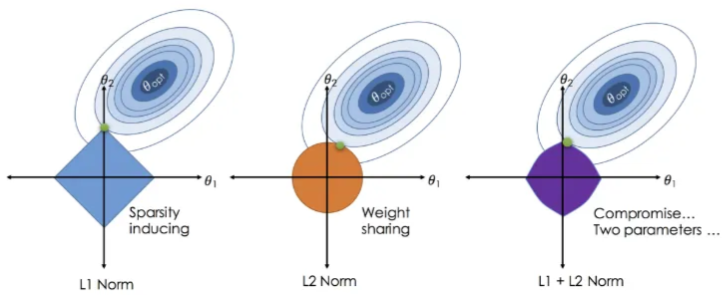
\includegraphics[scale=0.5]{img/regularizers.png}
      \caption{The ridge regularizer draws equipotential circles in our parameter space. The lasso draws a diamond, which tends to give a sparser solution since the loss is most likely to ``touch'' the corners of the contour plots of the regularizer. The elastic net is a linear combination of the ridge and lasso regularizers.} 
      \label{fig:regularizers_visual}
    \end{figure}

    To motivate this even further, let us take the two vectors 
    \begin{align}
      a = \bigg( \frac{1}{\sqrt{d}}, \ldots, \frac{1}{\sqrt{d}} \bigg) \qquad b = ( 1, 0, \ldots, 0)
    \end{align}
    Then the L0, L1, and L2 norms of $a$ are $d, \sqrt{d}, 1$ and those of $b$ are $1, 1, 1$. We want to choose a norm that capture the sparsity of $b$ and distinguishes it from $b$., The L0 norm clearly does this, but the L2 norm does not. The L1 norm is a good compromise between the two. 

    This now raises the question of how to determine a suitable regularization parameter $\lambda$. The next theorem shows a nice concentration property of the Lasso for bounded covariates. 

    \begin{theorem}[Concentration of Lasso]
      Given $(X, Y)$, assume that $|Y| \leq B$ and $\max_j |X_j| \leq B$. Let 
      \begin{equation}
        \beta^\ast = \argmin_{||\beta||_1 \leq L} r(\beta)
      \end{equation}
      be the best sparse linear predictor in the L1 sense, where $r(\beta) = \mathbb{E}[ (Y - \beta^T X)^2]$. Let our lasso estimator be 
      \begin{equation}
        \hat{\beta} = \argmin_{||\beta||_1 \leq L} \hat{r}(\beta) = \argmin_{||\beta||_1 \leq L} \frac{1}{n} \sum_{i=1}^n (Y_i - \beta^T X_i)^2
      \end{equation}
      which minimizes the empirical risk. Then, with probability at least $1 - \delta$, 
      \begin{equation}
        r(\hat{\beta}) \leq r(\beta^\ast) + \sqrt{\frac{16(L+1)^4 B^2}{n} \log \bigg( \frac{\sqrt{2} d}{\sqrt{\delta}} \bigg)} 
      \end{equation}
    \end{theorem}
    \begin{proof}
      
    \end{proof}

    \begin{code}[MWS of Lasso Regression in scikit-learn]
      \noindent\begin{minipage}{.6\textwidth}
      \begin{lstlisting}[]{Code}
        from sklearn.linear_model import Lasso

        X = np.random.randn(10, 5) 
        y = np.random.randn(10)
        # regularization parameter
        model = Lasso(alpha=1e-1)  
        model.fit(X, y) 
        print(model.score(X, y))  
        print(model.intercept_)
        print(model.coef_) 
        print(model.predict(np.array([[1, 2, 3, 4, 5]]))) 
      \end{lstlisting}
      \end{minipage}
      \hfill
      \begin{minipage}{.39\textwidth}
      \begin{lstlisting}[]{Output}
        0.47590269719236045
        -0.8861298412689853
        [0.         0.10767647 0.24172197 0.7427863  0.        ]
        [3.02553422]
        .
        .
        .
        .
        .
      \end{lstlisting}
      \end{minipage}
    \end{code}

    \subsubsection{Soft Thresholding and Proximal Gradient Descent} 

\section{Nonparametric Regression}

  \subsection{K Nearest Neighbors Regression}

    When we want to do nonparametric regression, i.e. when dealing with nonlinear functions, we can construct a function that uses local averaging of its nearby points. 

    \begin{example}[Local Averaging]
      Say that we want to fit some function through a series of datapoints in simple regression (one covariate). Then, what we can do is take some sliding window and our vale of the function at a point $x$ is the average of all values in the window $[x - \delta, x + \delta]$. 
      \begin{figure}[H]
        \centering 
        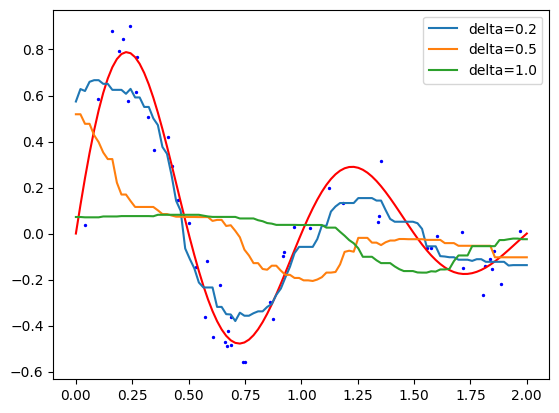
\includegraphics[scale=0.6]{img/kmeans_smoother.png}
        \caption{K means smoother} 
        \label{fig:kmeans_smoother}
      \end{figure}
    \end{example}

    \begin{code}[MWS of K Nearest Neighbor Regression in scikit-learn]
      Local averaging is implemented as the K nearest neighbor regressor in scikit learn. It is slightly different in the way that it doesn't use the points within a certain $\delta$ away but rather the $K$ nearest points. Either way, a minimal working example of this is 
      \begin{lstlisting}
        X = [[0], [1], [2], [3]]
        y = [0, 0, 1, 1]
        from sklearn.neighbors import KNeighborsRegressor
        neigh = KNeighborsRegressor(n_neighbors=2)
        neigh.fit(X, y)
        print(neigh.predict([[1.5]])) 
      \end{lstlisting}
    \end{code}

    Note that since $\hat{f}$ is a combination of step functions, this makes it discontinuous at points. 

  \subsection{Kernel Regression and Linear Smoothers} 

    K nearest neighbor regression puts equal weights on both near and far points, as long as they are in the window. This may not be ideal, so a simple modification is to \textit{weigh} these points according to their distance from the middle $x$. We can do this with a kernel, as the name suggests. Now this is not the same thing as a Mercer kernel in RKHS, so to distinguish that I will call it a \textit{local averaging kernel}. 

    \begin{definition}[Local Averaging Kernel]
      A \textbf{kernel} is any smooth, symmetric, and non-negative function $K : \mathbb{R} \to \mathbb{R}$.  
    \end{definition}

    \begin{definition}[Kernel Regression]
      Given some datapoints, $X$, our fitted regressor is of form 
      \begin{equation}
        \hat{f} (X) = \frac{\sum_{i} Y_i K \bigg( \frac{||X - X_i||}{h} \bigg)}{\sum_{i} K \bigg( \frac{||X - X_i||}{h} \bigg)}
      \end{equation}
      where $h$ is the \textbf{bandwidth} and the denominator is made sure so that the coefficients sum to $1$. To get a clearer picture, we are really taking the weighted average of the $Y_i$'s. 
      \begin{equation}
        \hat{f} (X) = \sum_{i} Y_i \ell_i (X) \text{ where } \sum_{i} \ell_i (X) = 1
      \end{equation}
      Denoting $Y = (Y_1, \ldots, Y_n) \in \mathbb{R}^n$ and the vector $f(X) = (f(X_1), \ldots, f(X_n))$, if we can write the kernel function as $\hat{Y} = \hat{f}(X) = S Y$, which in matrix form, is 
      \begin{equation}
        \begin{bmatrix} \hat{Y}_1 \\ \vdots \\ \hat{Y}_n \end{bmatrix} = \begin{bmatrix} \hat{f}(X_1) \\ \vdots \\ \hat{f} (X_n) \end{bmatrix} = \begin{bmatrix} \ell_1 (X_1) & \cdots & \ell_n (X_1) \\ \vdots & \ddots & \vdots \\ \ell_1 (X_n) & \cdots & \ell_n (X_n) \end{bmatrix} \begin{bmatrix} Y_1 \\ \vdots \\ Y_n \end{bmatrix} 
      \end{equation}
      then we say that we have a \textbf{linear smoother}, with stochastic matrix $S$ being our \textbf{smoothing matrix}. 
    \end{definition}

    The reason we'd like to have the weights to sum to $1$ is that if we had data that was constant (i.e. all $Y_i$'s are the same), then the fitted function should be constant at that value as well. Furthermore, the theme of linearity is important and will be recurring. The kernel estimator is defined for all $X$, but it's important to see its behavior at the training points $X_i$. The estimator $\hat{Y} = \hat{f}(X)$ is a linear combination of the $Y_i$'s, and the coefficients $\ell_i (X_j)$ depend on the values of $X_j$. Therefore, we have $\hat{Y} = S Y$, which is very similar to the equation $\hat{Y} = H Y$ in linear regression, where $H$ is the hat matrix that projects $Y$ onto the column space of $X$. Nonparametric regression has the same form, but rather than being a projection, it is a linear smoothing matrix. Therefore, this theme unifies both linear regression and nonparametric regression. Linear smoothers, spline smoother, Gaussian processes, are all just different choices of the smoothing matrix $S$. However, not all nonparametric estimators are linear smoothers, as we will see later. 

    Here are some popular kernels. 

    \begin{definition}[Gaussian Kernel]
      The \textbf{Gaussian kernel} is defined as 
      \begin{equation}
        K(x) = \frac{1}{\sqrt{2 \pi}} e^{-x^2/2}
      \end{equation}
      \begin{figure}[H]
        \centering 
        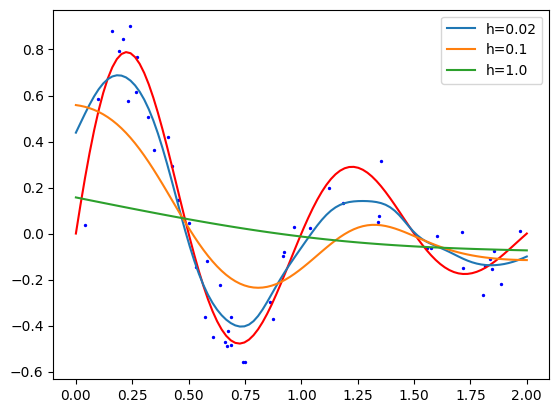
\includegraphics[scale=0.6]{img/gaussian_smoother.png}
        \caption{Gaussian kernel. } 
        \label{fig:gaussian_smoother}
      \end{figure}
    \end{definition}

    \begin{definition}[Box-Car Kernel]
      The \textbf{Box-Car kernel} is defined as 
      \begin{equation}
        K(x) = \frac{1}{2} \mathbbm{1}(|x| \leq 1)
      \end{equation}
      \begin{figure}[H]
        \centering 
        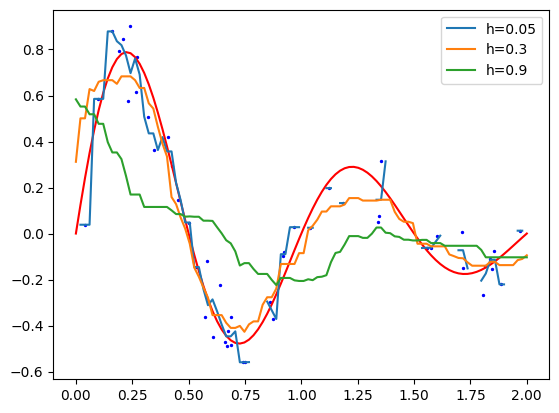
\includegraphics[scale=0.6]{img/boxcar_smoother.png}
        \caption{Boxcar kernel. } 
        \label{fig:boxcar_smoother}
      \end{figure}
    \end{definition}

    \begin{definition}[Epanechnikov Kernel]
      The \textbf{Epanechnikov kernel} is defined as 
      \begin{equation}
        K(x) = \frac{3}{4} (1 - x^2) \mathbbm{1}(|x| \leq 1)
      \end{equation}
      \begin{figure}[H]
        \centering 
        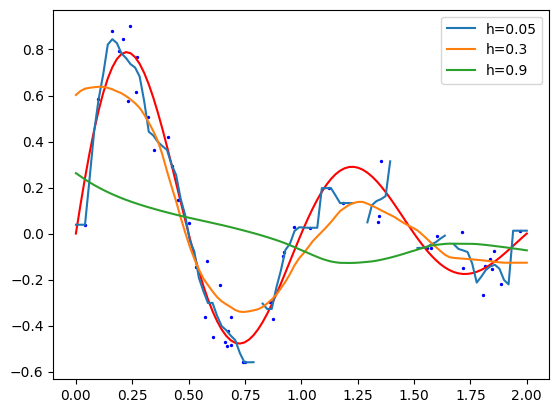
\includegraphics[scale=0.6]{img/epanechnikov_smoother.png}
        \caption{Epanechnikov kernel.} 
        \label{fig:epanechnikov_smoother}
      \end{figure}
    \end{definition}

    It turns out that from a theoretical point of view, the choice of the kernel doesn't really matter. What really matters is the bandwidth $h$ since that is what determines the bias variance tradeoff. To see why, if $h = 0$, then it will simply interpolate the points and variance is extremely high, and if $h = \infty$, then the fitted function will be constant at $\bar{Y}$, leading to high bias. The following theorem formalizes this.  

    \begin{theorem}[Bias Variance Tradeoff of Kernel Regression]
      Suppose that $d = 1$ and that $m^{\prime\prime}$ is bounded. Also suppose that $X$ has a nonzero, differentiable density $p$ and that the support is unbounded. Then, the risk is 
      \begin{align}
        R_n & = \frac{h_n^4}{4} \bigg( \int x^2 K(x) \bigg)^2 \int \bigg( m^{\prime\prime} (x) + 2m^\prime (x) \frac{p^\prime (x)}{p(x)} \bigg)^2 \,dx \\
            & \;\;\; + \frac{\sigma^2 \int K^2(x)\,dx} {n h_n} \int \frac{dx}{p(x)} + o \bigg( \frac{1}{n h_n} \bigg) + o(h_n^4) 
      \end{align}
      The first term is the squared bias and the second term is the variance. 
    \end{theorem}
    \begin{proof}
      We first denote 
      \begin{equation}
        \hat{f}(X) = \frac{\frac{1}{nh} \sum_{i=1}^n K \bigg( \frac{X - X_i}{h} \bigg) Y_i}{\frac{1}{nh} \sum_{i=1}^n K \bigg( \frac{X - X_i}{h} \bigg)} 
      \end{equation}
      where the denominator is the kernel density estimator $\hat{p}(X)$. Therefore, we rewrite
      \begin{align}
        \hat{f} (x) - f(x) & = \frac{\hat{a}(x)}{\hat{p}(x)} - f(x) \\
                           & = \bigg( \frac{\hat{a}(x)}{\hat{p}(x)} - f(x) \bigg) \bigg( \frac{\hat{p}(x)}{p(x) + 1 - \frac{\hat{p}(x)}{p(x)}} \bigg) \\
                           & = \frac{\hat{a}(x) - f(x) \hat{p}(x)}{p(x)} + \frac{(\hat{f}(x) - f(x)) (p(x) - \hat{p}(x))}{p(x)}
      \end{align}
      as $n \rightarrow \infty$ both $\hat{f}(x) - f(x)$ and $p(x) - \hat{p}(x)$ going to $0$, and since they're multiplied in the second term, it will go to $0$ very fast. So the dominant term is the first term, and we can write the above as approximately 
      \begin{equation}
        \hat{f}(x) - f(x) \approx  \frac{\hat{a}(x) - f(x) \hat{p}(x)}{p(x)}
      \end{equation}
      TBD continued. Wasserman lecture 6, 10:00. 
    \end{proof}

    From the theorem above, we can see that if the bandwidth is small, then $h^4$ is small and the bias decreases. However, there is a $h$ term in the denominator of the variance term, which also trades it off. We can furthermore see that the bias is sensitive to $p^\prime / p(x)$. This means that if the density is steep, then the bias will be high. This is known as \textit{design bias}, which is an underlying weakness in smoothing kernel regression. Another problem that is not contained in the theorem is the \textit{boundary bias}, which states that if you're near the boundary of the distribution (i.e. near the boundary of its support), then the bias also explodes. This happens to be very nasty especially in high dimensions where most of the data tends to be near the boundary. It turns out that this can be easily fixed with local polynomial regression, which gets rid of this term in the bias without any cost to variance. This means that this is unnecessary bias. 

    Then you can apply regularization on this to get kernel ridge regression. 

    \begin{code}[MWS of Kernel Ridge Regression in scikit learn]
      \begin{lstlisting}
        from sklearn.kernel_ridge import KernelRidge
        import numpy as np
        n_samples, n_features = 10, 5
        rng = np.random.RandomState(0)
        y = rng.randn(n_samples)
        X = rng.randn(n_samples, n_features)
        krr = KernelRidge(alpha=1.0)
        krr.fit(X, y)
      \end{lstlisting}
    \end{code}

  \subsection{Local Polynomial Regression}

    Now another way to think about the kernel estimator is as such. Suppose that you're doing linear regression on a bunch of points and you want to choose a $c$ that minimizes the loss. 
    \begin{equation}
      \sum_i (Y_i - c)^2
    \end{equation}
    You would just pick $c = \hat{Y}$. But if you are given some sort of locality condition, that the value of $c$ should depend more on the values closer to it, you're really now minimizing 
    \begin{equation}
      \sum_i (Y_i - c(x))^2 K \bigg( \frac{X_i - x}{h} \bigg)
    \end{equation}
    Minimizing this by setting the derivative equal to $0$ and solving gives us the kernel estimator. Therefore you're fitting some sort of local constant at a point $X$. But why fit a local constant, when you can fit a local line or polynomial? This is the idea behind local polynomial regression.

    \begin{figure}[H]
      \centering 
      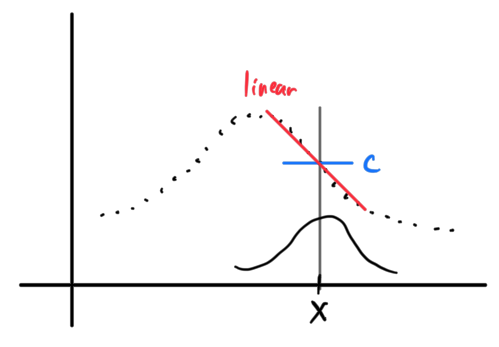
\includegraphics[scale=0.4]{img/local_linear_estimator.png}
      \caption{Rather than using a local constant, we can use a local linear estimator.} 
      \label{fig:local_linear_estimator}
    \end{figure}

    Therefore, we can minimize the modified loss. 

    \begin{definition}[Local Polynomial Estimator]
      The \textbf{local polynomial estimator} is a local linear kernel smoother that estimates the function $\hat{f}$ that minimizes the following loss. 
      \begin{equation}
        \argmin_{\beta} \sum_i K \bigg( \frac{X_i - x}{h} \bigg) \big( Y_i - (\beta_0 (x) - \beta_1 (x) (x- X_i) + \ldots + \beta_k (x) (x - X_i)^k )\big)
      \end{equation}
    \end{definition}

    So we can fit a line 
    \begin{equation}
      f(\mu) \approx \hat{\beta}_0 (x) + \hat{\beta}_1 (x) (\mu - x)
    \end{equation}
    and simply remove the intercept term to get the local linear estimator. 
    \begin{equation}
      \hat{f}(x) = \hat{\beta}_0 (x)
    \end{equation}
    Note that this is not the same as taking the constant estimate. We are extracting the fitted intercept term and so $\hat{\beta}_0(x) \neq c(x)$. 

    \begin{theorem}[Weighted Least Squares]
      The solution to the local linear estimator is similar to the weighted least squares solution. 
      \begin{equation}
        \hat{\beta}(x) = \begin{pmatrix} \hat{\beta}_0 (x) \\ \hat{\beta}_1 (x) \end{pmatrix} = (X^T W X)^{-1} X^T W Y
      \end{equation}
      where 
      \begin{equation}
        X = \begin{pmatrix} 1 & X_1 - x \\ \vdots & \vdots \\ 1 & X_n - x \end{pmatrix} \qquad W = \begin{pmatrix} K \bigg( \frac{X_1 - x}{h} \bigg) & 0 & \cdots & 0 \\ 0 & K \bigg( \frac{X_2 - x}{h} \bigg) & \cdots & 0 \\ \vdots & \vdots & \ddots & \vdots \\ 0 & 0 & \cdots & K \bigg( \frac{X_n - x}{h} \bigg) \end{pmatrix}
      \end{equation}
    \end{theorem}

    Computationally, it's similar to kernel regression and it gets rid of both the boundary and design bias. 

  \subsection{Regularized: Spline Smoothing}

    This is not local, but it's a linear smoother. 

  \subsection{Regularized: RKHS Regression}

    This is not local, but it's a linear smoother. 

  \subsection{Additive Models}

    In the most general case, we want to create nonparametric regression functions of the form 
    \begin{equation}
      Y = f(x_1, \ldots, x_d) + \epsilon 
    \end{equation}
    We've done this for one dimensional case, but we can extend this to multiple dimensions through additive models of the form 
    \begin{equation}
      Y = \sum_j f_j (x_j)  + \epsilon
    \end{equation}
    This gives us very interpretable models where we can clearly see the effect of each covariate on $Y$. Clearly, this is not as flexible as the previous model since they can't capture dependencies, but we can create sub-dependency functions and replace the form above to something like 
    \begin{equation}
      Y = \sum_{i, j} f_{i, j} (x_i, x_j) + \epsilon
    \end{equation}
    giving us more flexible models. 
  
  \subsection{Nonlinear Smoothers, Trend Filtering} 

    Tough example of the Dobbler function (like topologists sine curve). It's a pretty good fit but it's not too good since it's using a linear smoother (homogeneous). So we might need to fit it with nonlinear smoothers. 

  \subsection{High Dimensional Nonparametric Regression}

  \subsection{Regression Trees}

\section{Cross Validation} 

    We have understood the theoretical foundations of overfitting and underfitting with the bias variance decomposition. But in practice, we don't have an ensemble of datasets; we just have one. Therefore, we don't actually know what the bias, the variance, or the noise is at all. Therefore, how do we actually \textit{know} in practice when we are underfitting or overfitting? Easy. We just split our dataset into 2 different parts: the training set and testing sets. 
    \begin{equation}
      \mathcal{D} = \mathcal{D}_{train} \sqcup \mathcal{D}_{test}
    \end{equation}
    What we usually have is a \textbf{training set} that allows us to train the model, and then to check its performance we have a \textbf{test set}. We would train the model on the training set, where we will always minimize the loss, and then we would look at the loss on the test set. Though we haven't made a testing set, since we know the true model let us just generate more data and use that as our testing set. For each model, we can calculate the optimal $\boldsymbol{\theta}$, which we will denote $\boldsymbol{\theta}^\ast$, according to the \textbf{root mean squared loss}
    \begin{equation}
      h_{\boldsymbol{\theta}^\ast} = \argmin_{h_{\boldsymbol{\theta}}} \sqrt{ \frac{1}{N} \sum_{i=1}^N \big( y^{(i)} - h_{\boldsymbol{\theta}} (\mathbf{x}^{(i)}) \big)^2 }
    \end{equation}
    where division of $N$ allows us to compare different sizes of datasets on equal footing, and the square root ensures that this is scaled correctly. Let us see how well these different order models perform on a separate set of data generated by the same function with Gaussian noise. 

    \begin{figure}[H]
      \centering
      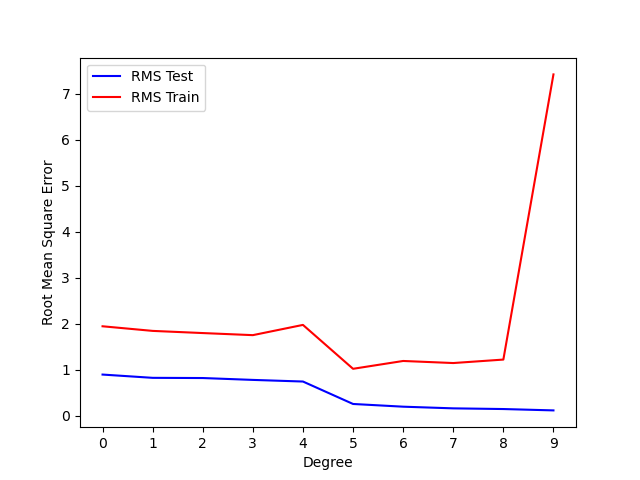
\includegraphics[scale=0.4]{img/Degree_vs_RMS.png}
      \caption{We can see that the RMS decreases monotonically on the training error as more complex functions become more fine-tuned to the data. However, when we have a $9$th degree polynomial the RMS for the testing set dramatically increases, meaning that this model does not predict the testing set well, and performance drops. }
      \label{fig:poly_deg_vs_rms}
    \end{figure}

    Now we know that a more complex model (i.e. that captures a greater set of functions) is not necessarily the best due to overfitting. Therefore, researchers perform \textbf{cross-validation} by taking the training set $(\mathcal{X}, \mathcal{Y})$. We divide it into $S$ equal pieces 
    \begin{equation}
      \bigcup_{s=1}^S D_s = (\mathcal{X}, \mathcal{Y})
    \end{equation}
    Then, we train the model $\mathcal{M}$ on $S-1$ pieces of the data and then test it across the final piece, and do this $S$ times for every test piece, averaging its perforance across all $S$ test runs. Therefore, for every model $\mathcal{M}_k$, we must train it $S$ times, for all $K$ models, requiring $KS$ training runs. If data is particularly scarce, we set $S = N$, called the \textbf{leave-one-out} technique. Then we just choose the model with the best average test performance. 

    The following result shows that cross-validation (data splitting) leads to an estimator with risk nearly as good as the best model in the class. 


    \begin{theorem}[Gyorfi, Kohler, Krzyak, Walk (2002)]
      Let $\mathcal{M} = \{m_h\}$ be a finite class of regression estimators indexed by a parameter $h$, with $m$ being the true risk minimizer, $m_{\hat{h}}$ being the empirical risk minimizer over the whole dataset $\mathcal{D}$, and $m_{H}$ being the empirical risk minimizer over the test set $\mathcal{D}_{\mathrm{test}}$ for ordinary least squares loss. 
      \begin{align}
        m_H & = \argmin_{m_h} \frac{1}{N} \sum_{i \in \mathcal{D}_{\mathrm{test}}} (y_i - m_h(x_i))^2 \\ 
        m_{\hat{h}} & = \argmin_{m_h} \frac{1}{N} \sum_{i \in \mathcal{D}} (y_i - m_h(x_i))^2 
      \end{align}
      If the data $Y_i$ and estimators are bounded by $L$, then for any $\delta > 0$, we have 
      \begin{equation}
        \mathbb{E} \int |m_H (x) - m(x)|^2 \,d\mathbb{P}(x) \leq (1 + \delta) \mathbb{E} \int |m_{\hat{h}} (x) - m(x) |^2 \,d \mathbb{P}(x) + \frac{C (1 + \log{|M|})}{n}
      \end{equation}
      where $c = L^2 (16/\delta + 35 + 19\delta)$. 
    \end{theorem}

    \begin{code}[Minimal Example of Train Test Split in scikit-learn]
      To implement this in scikit-learn, we want to use the \texttt{train\_test\_split} class. We can also set a random state parameter to reproduce results. 
      \begin{lstlisting}
        from sklearn.model_selection import train_test_split 

        # Split into training (80\%) and test (20\%) data 
        X_train, X_test, Y_train, Y_test = train_test_split(X, Y, test_size=0.2, random_state=66)
      \end{lstlisting}
    \end{code}

    However, this process requires a lot of training runs and therefore may be computationally infeasible. Therefore, various \textbf{information criterion} has been proposed to efficiently select a model. 

  \subsection{Leave 1 Out Cross Validation} 

    \subsubsection{Generalized (Approximate) Cross Validation} 

    \subsubsection{Cp Statistic}

  \subsection{K Fold Cross Validation}

  \subsection{Data Leakage}

  \subsection{Information Criterion}

\section{Linear Classification}

  \subsection{Empirical Risk Minimizer} 

    You literally just try to build a hyperplane to minimize the number of misclassifications, but this is not really differentiable and is hard. It's just a stepwise function. Therefore, you use a \textbf{surrogate loss function} to approximate the 0-1 loss function. The logistic uses some function, and the SVM uses the smallest convex function to approximate the 0-1 loss function. Here are some examples: 
    \begin{center}
      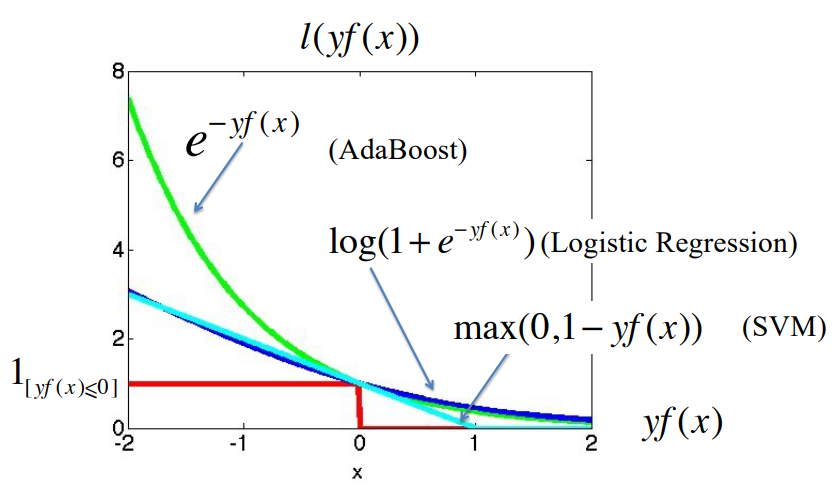
\includegraphics[scale=0.35]{img/loss_functions_class.png}
    \end{center}

  \subsection{Perceptron}

    \begin{definition}[Perceptron Model and Loss]
      The simplest binary classification model is the \textbf{perceptron algorithm}. It is a discriminative parametric model that assigns 
      \begin{equation}
        f_w (x) = \begin{cases} 1 & \text{ if } w^T x + b \geq 0 \\ -1 & \text { if } w^T x + b < 0 \end{cases}
      \end{equation}
      where we have chosen to label class $C_1 = 1$ and $C_2 = -1$. Note that unlike linear regression (and logistic regression, as we will see later), the perceptron is not a probabilistic model. It is a \textbf{discriminant function}, which just gives point estimates of the classes, not their respective probabilities. Like logistic regression, however, it is a linear model, meaning that the decision boundary it creates is always a linear (affine) hyperplane. 
    \end{definition}

    To construct the surrogate loss function, we would want a loss that penalizes not only if there is a misclassification, but how \textit{far} that misclassified point is from the boundary. Therefore, if $y$ and $\hat{y} = f_w (x)$ have the same sign, i.e. if $y f_w (x) > 0$, then the penalty should be $0$, and if it is $< 0$, then the penalty should be proportional to the orthogonal distance of the misclassified point to the boundary, which is represented by $-wT x y$ (where the negative sign makes this cost term positive). 

    \begin{definition}[Surrogate Loss for Perceptron]
      Therefore, our cost functions would take all the points and penalize all the terms by $0$ if they are correctly classified and by $-\mathbf{w}^T \boldsymbol{\phi}^{(n)} y^{(n)}$ if incorrectly classified. 
      \begin{equation}
        L(y, \hat{y}) = \sum_{n=1} [ -\mathbf{w}^T \boldsymbol{\phi}^{(n)} y^{(n)} ]_+ \text{ where } [f(\mathbf{x})]_+ \coloneqq \begin{cases} f(\mathbf{x}) & \text{ if } f(\mathbf{x}) > 0 \\ 0 & \text{ else } \end{cases}
      \end{equation}
      Note that this is a piecewise linear function and convex. 
    \end{definition}


    \begin{code}[Perceptron in scikit-learn]
      Let's implement this in scikit-learn, using two pipelines with different data standardization techniques to see the differences in the perceptron boundary. 

      \begin{figure}[H]
        \centering 
        \begin{lstlisting}
          from sklearn.pipeline import Pipeline 
          from sklearn.linear_model import Perceptron
          from sklearn.preprocessing import QuantileTransformer, StandardScaler

          pipe1 = Pipeline([ 
              ("scale", StandardScaler()), 
              ("model", Perceptron())
          ])

          pipe2 = Pipeline([
              ("scale", QuantileTransformer(n_quantiles=100)), 
              ("model", Perceptron())
          ])
        \end{lstlisting}
        \caption{} 
        \label{fig:Perceptron_Code}
      \end{figure}

      \begin{figure}[H]
        \centering
        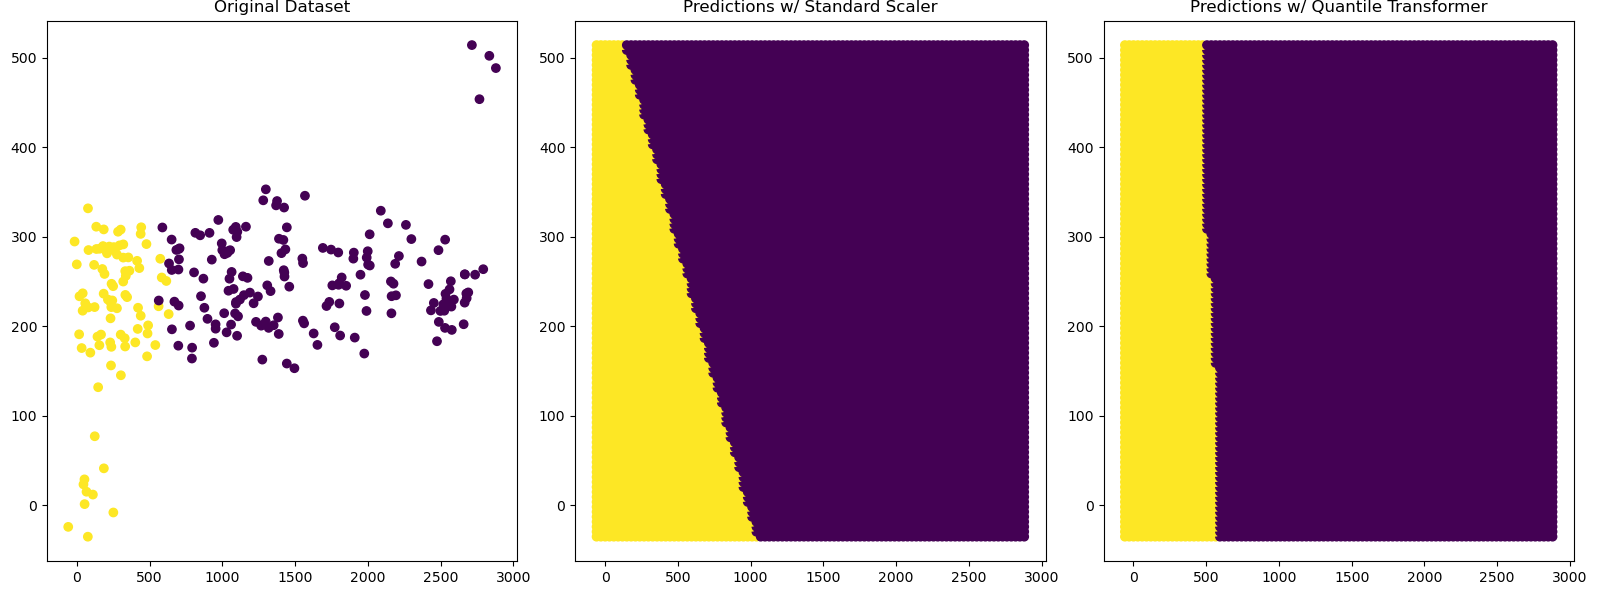
\includegraphics[scale=0.35]{img/Perceptron.png}
        \caption{Perceptron Trained on Different Standardized Data}
        \label{fig:Percepton_on_Standardized_data}
      \end{figure}
    \end{code}

  \subsection{Logistic and Softmax Regression} 

    We can upgrade from a discriminant function to a discriminative probabilistic model with \textbf{logistic regression}. In practice, we usually deal with \textbf{probabilistic models} where rather than giving a point estimate $\hat{y}$, we attempt to model the \textit{distribution} $\mathbb{P}_{Y \mid X = \hat{x}}$. Even though in the end, we will just output the mean $\mu$ of this conditional distribution, modeling the distribution allows us to quantify uncertainty in our measurements. 


    \begin{definition}[Logistic Regression]
      The \textbf{logistic regression} model is a linear model of the form 
      \begin{equation}
        f_w (x) = \sigma (w^T x) = \frac{1}{1 + e^{- w^T x}}, \text{ where } \sigma(x) \coloneqq \frac{1}{1 + e^{x}}
      \end{equation}
      It is different from linear regression in two ways: 
      \begin{enumerate}
        \item In linear regression, we assumed that the targets are linearly dependent with the covariates as $y = w^T x + b$. However, this means that the hypothesis $f_w$ is unbounded. Since we have two classes (say with labels $0$ and $1$), we must have some sort of \textit{link function} $\sigma$ that takes the real numbers and compresses it into the domain $[0, 1]$. Technically, we can choose any continuous, monotinically increasing function from $\mathbb{R}$ to $(0, 1)$. However, the following property of the sigmoid makes derivation of gradients very nice. 
          \begin{equation}
            \sigma^\prime (x) = \sigma(x) \, \big(1 - \sigma(x) \big)
          \end{equation}
        \item Once this is compressed, we assume that the residual distribution is a Bernoulli. 
      \end{enumerate}
    \end{definition}

    \begin{definition}[Binary Cross Entropy Loss as Surrogate Loss for Logistic Regression]
      The surrogate loss for logistic regression is the \textbf{binary cross entropy loss}, which is defined as
      \begin{equation}
        L(y, \hat{y}) = -y \log \hat{y} - (1 - y) \log (1 - \hat{y})
      \end{equation}
    \end{definition}

    One important observation to make is that notice that the output of our hypothesis is used as a parameter to define our residual distribution. 
    \begin{enumerate}
      \item In linear regression, the $f_w$ was used as the \textit{mean} $\mu$ of a Gaussian. 
      \item In logistic regression, the $f_w$ is used also as the mean $p$ of a Bernoulli. 
    \end{enumerate}
    The reason we want this sigmoid is so that we make the domains of the means of the residuals match the range of the outputs of our model. It's simply a manner of convenience, and in fact we could have really chose any function that maps $\mathbb{R}$ to $(0, 1)$. 

    Some questions may arise, such as ``why isn't the variance parameter of the Gaussian considered in the linear model?" or ``what about other residual distributions that have multiple parameters?" This is all answered by generalized linear models, which uses the output of a linear model as a \textit{natural parameter} of the canonical exponential family of residual distributions. 

    Unfortunately, there is no closed form solution for logistic regression like the least squares solution in linear regression. Therefore, we can only resort to maximum likelihood estimation. 

    \begin{theorem}[Maximum Likelihood Estimation for Logistic]
      Given a dataset $\mathcal{D} = \{(x^{(i)}, y^{(i)})\}_{i=1}^N$, our likelihood is 
      \[L(\theta ; \mathcal{D}) = \prod_{i=1}^n p(y^{(i)} \;|\; x^{(i)} ; \theta) = \prod_{i=1}^N  \big( h_\theta (x^{(i)} )\big)^{y^{(i)}} \; \big( 1 - h_\theta (x^{(i)})\big)^{1-y^{(i)}}\]
      We can equivalently minimize its negative log likelihood, giving us the \textbf{binary cross entropy} loss function
      \begin{align*}
          \ell(\theta) & = -\log L(\theta) \\
          & = -\sum_{i=1}^n y^{(i)} \log h_\theta (x^{(i)}) + (1 - y^{(i)}) \log (1 - h_\theta (x^{(i)}))
      \end{align*}
      Now taking the gradient for just a single sample $(x^{(i)}, y^{(i)})$ gives 
      \begin{align*}
          \frac{\partial \ell}{\partial \theta}  & = \bigg( \frac{y^{(i)}}{\sigma(\theta^T x^{(i)})} - \frac{1 - y^{(i)}}{1 - \sigma(\theta^T x^{(i)})} \bigg) \, \frac{\partial}{\partial \theta} \sigma (\theta^T x^{(i)}) \\
          & = \frac{\sigma(\theta^T x^{(i)}) - y^{(i)}}{\sigma(\theta^T x^{(i)}) \, \big( 1 - \sigma(\theta^T x^{(i)}) \big)} \sigma(\theta^T x^{(i)}) \, \big( 1 - \sigma(\theta^T x^{(i)}) \big) x^{(i)} \\
          & = \big( h_\theta (x^{(i)}) - y^{(i)} \big) x
      \end{align*}
      and summing it over some minibatch $M \subset \mathcal{D}$ gives 
      \[\nabla_\theta \ell_M = \sum_{(x, y) \in M} (y - h_\theta(x)) x\]
      Therefore, the stochastic gradient descent algorithm is 
      \begin{align*}
          \theta & = \theta - \eta \nabla_\theta \ell (\theta) \\
          & = \theta - \eta \sum_{(x, y) \in M} (y - h_\theta(x)) x
      \end{align*}
    \end{theorem}

    We would like to extend this to the multiclass case. 

    \begin{definition}[Softmax Function]
      The softmax function is defined 
      \begin{equation}
      o(\mathbf{x}) = \frac{e^{\mathbf{x}}}{||e^{\mathbf{x}}||} = \frac{1}{\sum_j e^{x_j}}\begin{pmatrix} e^{x_1} \\ \vdots \\ e^{x_D} \end{pmatrix}
      \end{equation}
    \end{definition}

    What makes the softmax so popular is that the total derivative turns out to simplify functions a lot. The total derivative of the softmax can be derived as such. 

    \begin{lemma}[Derivative of Softmax]
      The derivative of the softmax is 
      \begin{equation}
        D o (\mathbf{x}) = \mathrm{diag}(o (\mathbf{x})) - o (\mathbf{x}) \otimes o (\mathbf{x})
      \end{equation}
      where $\otimes$ is the outer product. That is, let $y_i$ be the output of the softmax. Then, for the $4 \times 4$ softmax function, we have 
      \begin{equation}
        D o(\mathbf{x}) = \begin{pmatrix} y_1 (1 - y_1) & - y_1 y_2 & -y_1 y_3 & - y_1 y_4 \\ -y_2 y_1 & y_2 (1 - y_2) & - y_2 y_3 & - y_2 y_4 \\ -y_3 y_1 & y_3 y_3 & y_3 (1 - y_3) & -y_3 y_4 \\ -y_4 y_1 & -y_4 y_2 & -y_4 y_3 & y_4 (1 - y_4) \end{pmatrix}
      \end{equation}
    \end{lemma}
    \begin{proof}
      We will provide a way that allows us not to use quotient rule. Given that we are taking the partial derivative of $y_i$ with respect to $x_j$, we can use the log of it to get 
      \[\frac{\partial}{\partial x_j} \log (y_i) = \frac{1}{y_i} \frac{\partial y_i}{\partial x_j} \implies \frac{\partial y_i}{\partial x_j} = y_i \, \frac{\partial}{\partial x_j} \log(y_i)\]
      Now the partial of the log term is 
      \begin{align*}
        \log{y_i} & = \log \bigg( \frac{e^{x_i}}{\sum_l e^{x_l}} = x_i - \log \bigg( \sum_l e^{x_l}\bigg) \\
        \frac{\partial}{\partial x_j} \log(y_i) & = \frac{\partial x_i}{\partial x_j} - \frac{\partial}{\partial x_j} \log \bigg( \sum_l e^{x_l}\bigg) \\
        & = 1_{i = j} - \frac{1}{\sum_l e^{x_l}} e^{x_j}
      \end{align*}
      and plugging this back in gives 
      \begin{equation}
        \frac{\partial y_i}{\partial x_j} = y_i (1_{i = j} - y_j)
      \end{equation}
    \end{proof}

    It also turns out that the sigmoid is a specific case of the softmax. That is, given softmax for 2 classes, we have 
    \[o\begin{pmatrix} x_1 \\ x_2 \end{pmatrix} = \frac{1}{e^{x_1} + e^{x_2}} \begin{pmatrix} e^{x_1} \\ e^{x_2} \end{pmatrix}\]
    So, the probability of being in class $1$ is 
    \[\frac{e^{x_1}}{e^{x_1} + e^{x_2}} = \frac{1}{1 + e^{x_2 - x_1}}\]
    and the logistic sigmoid is just a special case of the softmax function that avoids using redundant parameters. We actually end up overparameterizing the softmax because the probabilities must add up to one. 

    \begin{definition}[Softmax Regression Model]
      The softmax regression of $K$ classes assumes a model of the form 
      \begin{equation}
        h_\theta (x) = o ( \mathbf{W} \mathbf{x} + \mathbf{b})
      \end{equation}
      where $\mathbf{W} \in \mathbb{R}^{K \times D}, \mathbf{b} \in \mathbb{R}^D$. Again, we have a linear map followed by some link function (the softmax) which allows us to nonlinearly map our unbounded linear outputs to some domain that can be easily parameterized by a probability distribution. In this case, our residual distribution is a \textbf{multinomial distribution} 
      \begin{equation}
        y \sim \mathrm{Multinomial}\big( h_\mathbf{w} (\mathbf{x}) \big) = \mathrm{Multinomial}\big( [h_\mathbf{w} (\mathbf{x})]_1, \ldots, [h_\mathbf{w} (\mathbf{x})]_K \big)
      \end{equation}
    \end{definition}

    \begin{definition}[Multiclass Cross Entropy Loss as Surrogate Loss for Softmax]
      The surrogate loss for softmax regression is the \textbf{multiclass cross entropy loss}, which is defined as 
      \begin{equation}
        L(\theta ; \mathcal{D}) = - \sum_{i=1}^N \sum_{k=1}^K y_k^{(i)} \log \big( h_\theta (\mathbf{x}^{(i)}) \big)_k
      \end{equation}
    \end{definition}

    \begin{theorem}[Maximum Likelihood Estimation for Softmax]
      Since a closed form solution is not available for logistic regression, it is clearly not available for softmax. Therefore, we one hot encode our target variables as $\mathbf{y}^{(i)}$ and write our likelihood as 
      \begin{equation}
        L(\theta; \mathcal{D}) = \prod_{i=1}^N \prod_{k=1}^K p(C_k \mid \mathbf{x}^{(i)})^{\mathbf{y}^{(i)}_k} = \prod_{i=1}^N \prod_{k=1}^K \big( \mathbf{h}_\mathbf{W} (\mathbf{x}^{(i)})\big)_k^{\mathbf{y}_k^{(i)}}
      \end{equation}
      Taking the negative logarithm gives us the \textbf{cross entropy} loss function
      \begin{equation}
        \ell (\boldsymbol{\theta}) = - \sum_{i=1}^N \sum_{k=1}^K y^{(i)}_k \log \big( \mathbf{h}_{\boldsymbol{\theta}} (\mathbf{x}^{(i)})\big)_k = - \sum_{i=1}^N \mathbf{y}^{(i)} \dot \log \big( \mathbf{h}_{\boldsymbol{\theta}} (\mathbf{x}^{(i)} \big)
      \end{equation}
      where $\cdot$ is the dot product. The gradient of this function may seem daunting, but it turns out to be very cute. Let us take a single sample $(\mathbf{x}^{(i)}, \mathbf{y}^{(i)})$, drop the index $i$, and write
      \begin{align*}
        \mathbf{x} & \mapsto \mathbf{W} \mathbf{x} + \mathbf{b} = \mathbf{z} \\
        \hat{\mathbf{y}} = \mathbf{a} & = o (\mathbf{z}) \\
        L & = - \mathbf{y} \cdot \log (\mathbf{a}) = - \sum_{k=1}^K y_k \log(a_k)
      \end{align*}
      We must compute 
      \[\frac{\partial L}{\partial \mathbf{W}} = \frac{\partial L}{\partial \mathbf{a}} \frac{\partial \mathbf{a}}{\partial \mathbf{z}} \frac{\partial \mathbf{z}}{\partial \boldsymbol{\theta}}\]
      We can compute $\partial L /\partial \mathbf{z}$ as such, using our derivations for the softmax derivative above. We compute element wise. 
      \begin{align*}
        \frac{\partial L}{\partial z_j} & = - \sum_{k=1}^K y_k \, \frac{\partial}{\partial z_j} \log (a_k) \\
        & = - \sum_{k=1}^K y_k \frac{1}{a_k} \frac{\partial a_k}{\partial z_j} \\
        & = - \sum_{k=1}^K \frac{y_k}{a_k} \, a_k (1_{\{k = j\}} - a_j) \\
        & = - \sum_{k=1}^K y_k (1_{\{k = j\}} - a_j) \\
        & = \bigg( \sum_{k=1}^K y_k a_j \bigg) - y_j \\
        & = a_j \bigg( \sum_{k=1}^K y_k \bigg) - y_j \\
        & = a_j - y_j
      \end{align*}
      and combining these gives 
      \begin{equation}
        \frac{\partial L}{\partial \mathbf{z}} = (\mathbf{a} - \mathbf{y})^T
      \end{equation}
      Now, computing $\partial \mathbf{z} / \partial \mathbf{W}$ gives us a $3$-tensor, which is not ideal to work with. However, let us just compute this with respect to the elements again. We have 
      \begin{align*}
        z_k & = \sum_{d=1}^D W_{kd} x_d + b_k \\ 
        \frac{\partial z_k}{\partial W_{ij}} & = \sum_{d=1}^D x_d \frac{\partial}{\partial W_{ij}} W_{kd}
      \end{align*}
      where 
      \begin{equation}
        \frac{\partial}{\partial W_{ij}} W_{kd} = \begin{cases} 1 & \text{ if } i = k, j = d \\ 0 & \text{ else} \end{cases}
      \end{equation}
      Therefore, since $d$ is iterating through all elements, the sum will only be nonzero if $k = i$. That is, $\frac{\partial z_k}{\partial W_{ij}} = x_j$ if $k = i$ and $0$ if else. Therefore, 
      \begin{center}
        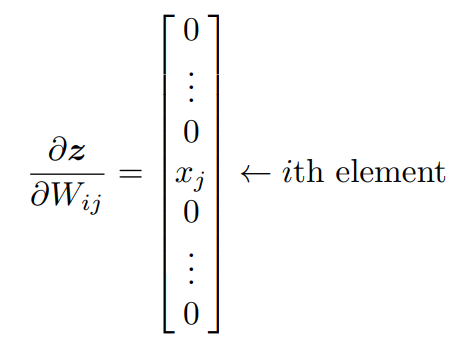
\includegraphics[scale=0.3]{img/softmax_deriv.png}
      \end{center}
      Now computing 
      \begin{equation}
        \frac{\partial L}{\partial W_{ij}} = \frac{\partial L}{\partial \mathbf{z}} \frac{\partial \mathbf{z}}{\partial W_{ij}} = (\mathbf{a} - \mathbf{y}) \frac{\partial \mathbf{z}}{\partial W_{ij}} = \sum_{k=1}^K (a_k - y_k) \frac{\partial z_k}{\partial W_{ij}} = (a_i - y_i) x_j
      \end{equation}
      To get $\partial L / \partial W_{ij}$ we want a matrix whose entry $(i, j)$ is $(a_i - y_i) x_j$. This is simply the outer product as shown below. For the bias term, $\partial \mathbf{z} / \partial \mathbf{b}$ is simply the identity matrix. 
      \begin{equation}
        \frac{\partial L}{\partial \mathbf{W}} = (\mathbf{a} - \mathbf{y}) \mathbf{x}^T, \;\;\;\; \frac{\partial L}{\partial \mathbf{b}} = \mathbf{a} - \mathbf{y}
      \end{equation}

      Therefore, summing the gradient over some minibatch $M \subset [N]$ gives 
      \begin{equation}
        \nabla_{\mathbf{W}} \ell_M = \sum_{i \in M} (\mathbf{h}_{\boldsymbol{\theta}}(\mathbf{x}^{(i)}) - \mathbf{y}^{(i)}) (\mathbf{x}^{(i)})^T, \;\;\;\;\; \nabla_{\mathbf{b}} \ell_M = \sum_{i \in M} (\mathbf{h}_{\boldsymbol{\theta}}(\mathbf{x}^{(i)}) - \mathbf{y}^{(i)})
      \end{equation}
      and our stochastic gradient descent algorithm is 
      \begin{align*}
        \boldsymbol{\theta} = \begin{pmatrix} \mathbf{W} \\ \mathbf{b} \end{pmatrix} & = \begin{pmatrix} \mathbf{W} \\ \mathbf{b} \end{pmatrix} - \eta \begin{pmatrix} \nabla_{\mathbf{W}} \ell_M \\ \nabla_{\mathbf{b}} \ell_M \end{pmatrix} \\
        & = \begin{pmatrix} \mathbf{W} \\ \mathbf{b} \end{pmatrix} - \eta \begin{pmatrix} \sum_{i \in M} (\mathbf{h}_{\boldsymbol{\theta}}(\mathbf{x}^{(i)}) - \mathbf{y}^{(i)}) (\mathbf{x}^{(i)})^T \\ \sum_{i \in M} (\mathbf{h}_{\boldsymbol{\theta}}(\mathbf{x}^{(i)}) - \mathbf{y}^{(i)}) \end{pmatrix} 
      \end{align*}
    \end{theorem}

    \subsubsection{Sparse Logistic Regression}

  \subsection{Support Vector Machines}

    \begin{definition}[Hinge Loss]
      The \textbf{hinge loss} is a convex surrogate loss function for the 0-1 loss function. It is defined as 
      \begin{equation}
        L(y, \hat{y}) = \max(0, 1 - y \cdot \hat{y})
      \end{equation}
    \end{definition}

    A support vector machine focuses only on the points that are most difficult to tell apart, whereas other classifiers pay attention all of the points. A SVM is a discriminative, non-probabilistic model. Let us first assume that our dataset $\mathcal{D} = \{\mathbf{x}_i, y_i\}$ is linearly separable with $y_i \in \{-1, +1\}$. Based on previous algorithms like the perceptron, it will find some separating hyperplane. However, there's an infinite number of separating hyperplanes as shown in Figure \ref{fig:svm_intro_1}. What support vector machines want to do is to find the best one, with the ``best" defined as the hyperplane that maximizes the distance between either the closest positive or negative samples, shown in Figure $\ref{fig:svm_intro2}$.  

    \begin{figure}[H] 
      \centering 
      \begin{subfigure}[b]{0.45\textwidth} 
        \centering 
        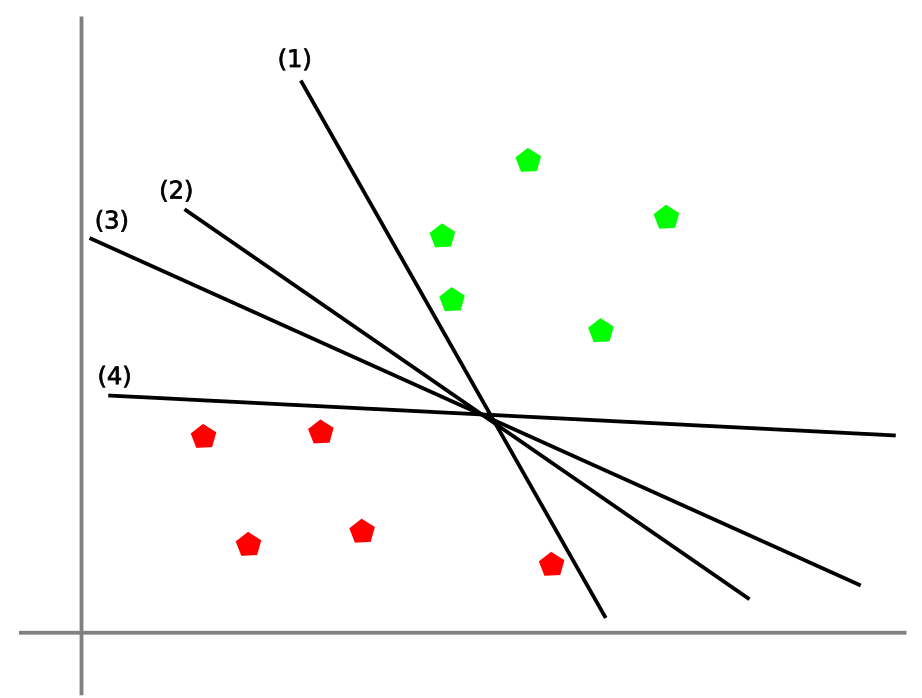
\includegraphics[width=\textwidth]{img/svm_intro.png} 
        \caption{Planes such as (1) and (4) are ``too close" to the positive and negative samples. } 
        \label{fig:svm_intro_1}
      \end{subfigure}
      \hfill
      \begin{subfigure}[b]{0.45\textwidth} 
        \centering 
        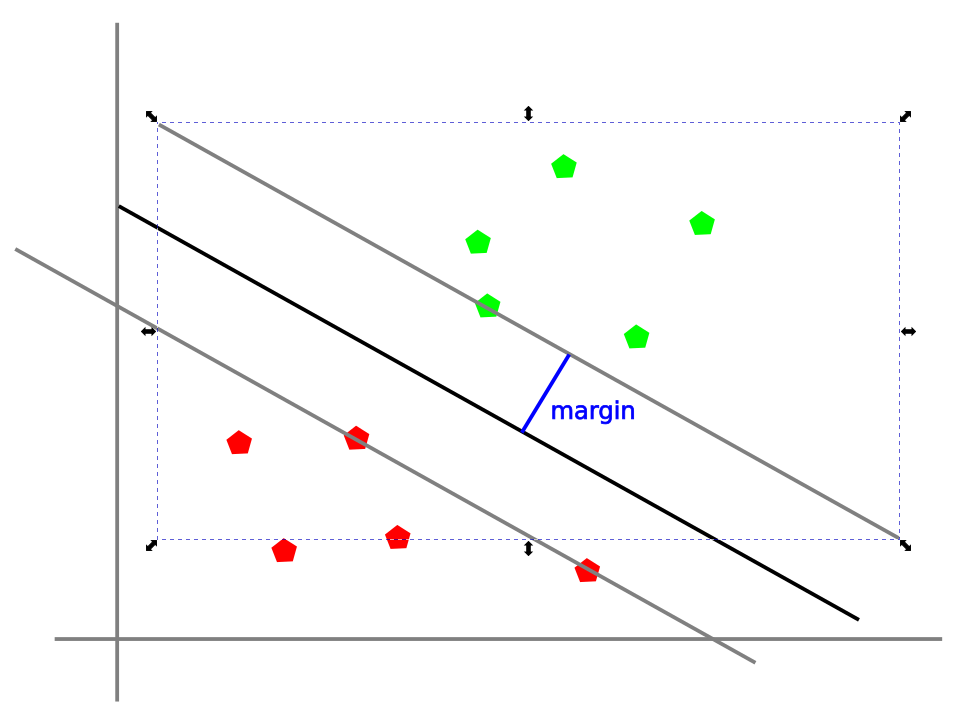
\includegraphics[width=\textwidth]{img/svm_intro_2.png}  
        \caption{SVMs try to find the separating hyperplane with the best minimum margin.} 
        \label{fig:svm_intro2}
      \end{subfigure} 
      \caption{Motivating problem} 
      \label{fig:svm_intro} 
    \end{figure}

    We want to formalize the concepts of these margins that we wish to maximize. To do this, we will define two terms. 

    \begin{definition}[Geometric margin]
      Given a point $\mathbf{x}_0$ and a hyperplane of equation $\mathbf{w} \cdot \mathbf{x} + b = 0$, the distance from $\mathbf{x}_0$ to the hyperplane, known as the \textbf{geometric margin}, can be computed with the formula 

      \begin{equation}
        d = \frac{|\mathbf{x}_0 \cdot \mathbf{w} + b|}{||\mathbf{w}||}  
      \end{equation} 

      Therefore, the geometric margin of the $i$th sample with respect to the hypothesis $f$ is defined 

      \begin{equation}
        \gamma_i = \frac{y_i \, (\mathbf{w} \cdot \mathbf{x}_i + b)}{||\mathbf{w}||} 
      \end{equation} 
    \end{definition}

    We wish to optimize the parameters $\mathbf{w}, b$ in order to maximize the minimum of the geometric margins (the distance between the closest point and the hyperplane). 

    \begin{equation}
      \argmax_{\mathbf{w}, b} \min_i \gamma_i = \argmax_{\mathbf{w}, b} \bigg\{ \frac{1}{||\mathbf{w}||} \min_i \big[y_i \, (\mathbf{w} \cdot \mathbf{x}_i + b) \big] \bigg\}
    \end{equation}

    Direct solution of this optimization problem would be very complex, and so we convert this into an equivalent problem that is much easier to solve. Note that the solution to the above term is not unique. If there was a solution $(\mathbf{w}^\ast, b^\ast)$, then 

    \begin{equation}
      \frac{y_i (\mathbf{w} \cdot \mathbf{x}_i + b)}{||\mathbf{w}||} = \frac{y_i (\lambda \mathbf{w} \cdot \mathbf{x}_i + \lambda b)}{||\lambda \mathbf{w}||}  
    \end{equation}

    That is, the geometric margin is not sensitive to scaling of the parameters of the hyperplane. Therefore, we can scale the numerator and the denominator by whatever we want and use this freedom to set 

    \begin{equation*}
      y_i ( \mathbf{w} \cdot \mathbf{x}_i + b ) = 1 
    \end{equation*}
    
    for the point that is closest to the surface. In that case, all data points will satisfy the constraints 

    \begin{equation*}
      y_n (\mathbf{w} \cdot \mathbf{x}_i + b) \geq 1
    \end{equation*}

    In the case of data points for which the equality holds, the constraints are said to be \textit{active}, whereas for the remainder they are \textit{inactive}. Therefore, it will always be the case that $\min_i \big[ y_i \, (\mathbf{w} \cdot \mathbf{x}_i + b)\big] = 1$, and the constraint problem reduces to 

    \begin{equation*}
      \argmax_{\mathbf{w}, b} \frac{1}{||\mathbf{w}||} = \argmin_{\mathbf{w}, b} \frac{1}{2} ||\mathbf{w}||^2 \text{ subject to constraints } y_i (\mathbf{w} \cdot \mathbf{x}_i + b) \geq 1 
    \end{equation*}

    This final step is the most significant step in this derivation and may be hard to wrap around the first time. So we dedicate the next subsubsection for this. 

    \subsection{Functional and Geometric Margins} 

    We could just work straight with this geometric margin, but for now, let's try to extend what we did with the perceptron into SVMs. We will find out that extending the concept of functional margins into SVMs leads to ill-defined problems. In the perceptron, we wanted to construct a function $f(\mathbf{x}) = \mathbf{w} \cdot \mathbf{x} + b$ such that 
    \begin{equation*}
      y_i \, f(\mathbf{x}_i) \geq 0 \text{ for all } i = 1, 2, \ldots, N
    \end{equation*}

    \begin{definition}[Functional Margin]
      The value of $y_i \, f(\mathbf{x}_i)$ gives us our confidence on our classification, and in a way it represents a kind of distance away from the separating hyperplane (if this value was $0$, then we would be 50 50 split on whether to label it positive or negative). Therefore, we shall define 
      \begin{equation*}
          \hat{\gamma}_i = y_i f(\mathbf{x}_i) 
      \end{equation*}
    as the \textbf{functional margin} of $(\mathbf{w}, b)$ with respect to the training sample $(\mathbf{x}_i, y_i)$. Therefore, the smallest of the function margins can be written 
    \begin{equation*}
        \hat{\gamma} = \min_i \gamma_i 
    \end{equation*}
    called the \textbf{function margin}. 
    \end{definition}

    Note that the geometric margin and functional margin are related by a constant scaling factor. Given a sample $(\mathbf{x}_i, y_i)$, we have 
    \begin{equation*}
        \mathrm{Geometric Margin} = \frac{y_i \, (\mathbf{w} \cdot \mathbf{x}_i + b)}{||\mathbf{w}||_2} = \frac{\mathrm{Functional Margin}}{||\mathbf{w}||_2}
    \end{equation*}

    As we can see, the perceptron works with the functional margin, and since it does not care about how large the margin is (just whether it's positive or negative), we are left with an underdetermined system in which there exists infinite $(\mathbf{w}, b)$'s. Now what we want to do is impose a certain minimum margin $\gamma > 0$ and solve for $(\mathbf{w}, b)$ again, and keep increasing this $\gamma$ until there is some unique solution. We can view this problem in two ways: 
    \begin{enumerate} 
        \item Take a specific minimum margin $\gamma$ and find a $(\mathbf{w}, b)$, which may not exist, be unique, or exist infinitely that satisfies 
            \begin{equation*}
                y_i f(\mathbf{x}) = y_i ( \mathbf{w} \cdot \mathbf{x} + b) \geq \gamma \text{ for all } i = 1, \ldots, N 
            \end{equation*}
        \item Take a specific $(\mathbf{w}, b)$ and calculate the maximum $\gamma$ that satisfies the constraint equations above.  
    \end{enumerate}

    They're both equivalent problems, but both ill-posed if we look at (2). Since the samples are linearly separable by assumption, we can say that there exists some $\epsilon > 0$ such that $y_i f(\mathbf{x}_i) \geq \epsilon$ for all $i$. Therefore, if we just scale $(\mathbf{w}, b) \mapsto (\lambda \mathbf{w}, \lambda b)$ for some large $\lambda$, this leads to the solution for $\gamma$ being unbounded. We can see in Figure $\ref{fig:scaling_problem}$ that we can increased confidence at no cost. Looking at (1), we can also see that if $(\mathbf{w}, b)$ does exist, then every other $(\lambda \mathbf{w}, \lambda b)$ for $\lambda > 1$ satisfies the property.   

    \begin{figure}[H] 
      \centering 
      \begin{subfigure}[b]{0.32\textwidth} 
        \centering 
        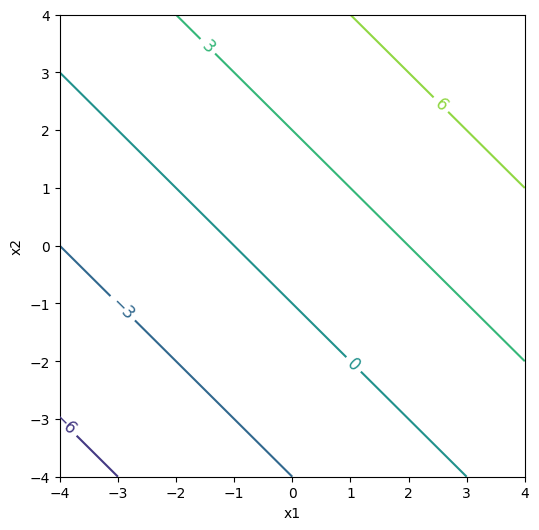
\includegraphics[width=\textwidth]{img/scaling1.png} 
        \caption{$f(x) = x_1 + x_2 + 1$} 
        \label{fig:original_scaled}
      \end{subfigure} 
      \hfill    
      \begin{subfigure}[b]{0.32\textwidth} 
        \centering 
        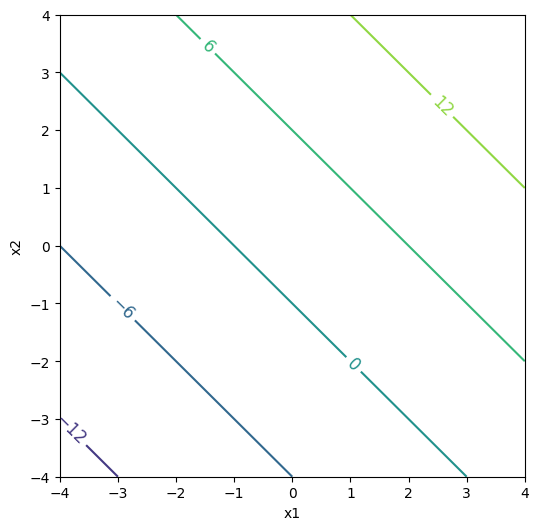
\includegraphics[width=\textwidth]{img/scaling2.png} 
        \caption{$f(x) = 2 x_1 + 2 x_2 + 2$} 
        \label{fig:two_times_scaled}
      \end{subfigure} 
      \hfill
      \begin{subfigure}[b]{0.32\textwidth} 
        \centering 
        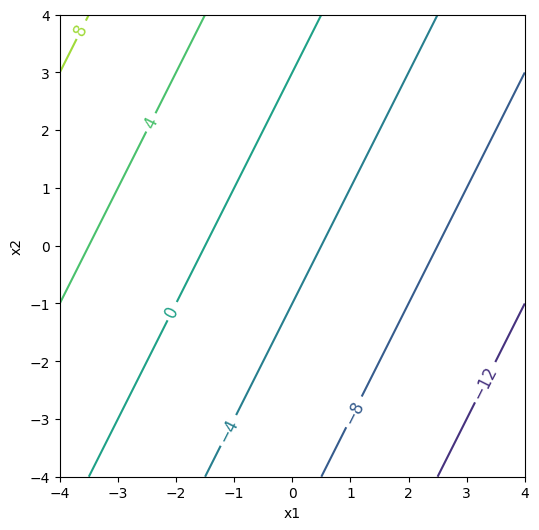
\includegraphics[width=\textwidth]{img/scaling3.png} 
        \caption{$f(x) = -2x_1 + x_2 - 3$} 
        \label{fig:something_else}
      \end{subfigure} 
      \caption{From (a), you can see that simply multiplying everything by two automatically increases our confidence by $2$, meaning that the functional margin can be scaled arbitrarily by scaing $(\mathbf{w}, b)$. There are still too many degrees of freedom in here and so extra constraints must be imposed. } 
      \label{fig:scaling_problem} 
    \end{figure}

    \subsubsection{Lagrange Duality} 

      To minimize the equations with the constraint equations, we can use the method of Lagrange multipliers, which leads to to Lagrangian 
      \[\mathcal{L}(\mathbf{w}, b, \boldsymbol{\alpha}) = \frac{1}{2} ||\mathbf{w}||^2 - \sum_i \alpha_i \big[ y_i (\mathbf{w} \cdot \mathbf{x}_i + b) - 1\big]\]
      We can take the gradients with respect to $\mathbf{w}$ and $b$ and set them to $0$, which gives the two conditions 
      \begin{align*} 
        \mathbf{w} & = \sum_i \alpha_i y_i \mathbf{x}_i \\
        0 & = \sum_i \alpha_i y_i \mathbf{x}_i 
      \end{align*}

      Now let's substitute our evaluated $\mathbf{w}$ back into $\mathcal{L}$, which gives the \textbf{dual representation} of the maximum margin problem in which we maximize  
      \begin{align*} 
          L & = \frac{1}{2} \bigg( \sum_i \alpha_i y_i \mathbf{x}_i \bigg) \bigg( \sum_j \alpha_j y_j \mathbf{x}_j \bigg) - \sum_{i} \alpha_i y_i x_i \cdot \bigg[ \sum_j \alpha_j y_j x_j \bigg] - \sum_i \alpha_i y_i b + \sum_i \alpha_i \\ 
            & = \sum_i \alpha_i - \frac{1}{2} \sum_{i, j} \alpha_i \alpha_j y_i y_j \, \mathbf{x}_i \cdot \mathbf{x}_j 
      \end{align*}
      The summation with the $b$ in it is $0$ since we can pull the $b$ out and the remaining sum is $0$ from before. Now the optimization only depends on the dot product $\mathbf{x}_i \cdot \mathbf{x}_j$ of all pairs of sample vectors, which is very interesting. We will see more of this when we talk about kernel methods. Now, we need to solve the dual problem 
      \[\max_{\boldsymbol{\alpha}} \mathcal{L}(\boldsymbol{\alpha})\]
      which can be done using some generic quadratic programming solver or some other method to get the optimum $\boldsymbol{\alpha}^\ast$, which gives us 
      \[\mathbf{w}^\ast = \sum_i \alpha_i^\ast y_i \mathbf{x}_i\]


    \subsection{Nonseparable Case} 

  \subsection{Gaussian/Linear Discriminant Analysis}

    \subsubsection{Discriminative vs. Generative Models}

      Now we introduce our first example of a generative model, which introduces another division between models (in addition to parametric vs nonparametric, frequentist vs bayesian). Generally, there are two ways to model $\mathbb{P}_{Y \mid X = x}$. 

      \begin{definition}[Discriminative Models]
        \textbf{Discriminative models} attempt to do this directly by  modeling only the conditional probability distribution $\mathbb{P}_{Y \mid X = x}$. We don't care about the underlying distribution of $X$, but rather we just want to try and predict $Y$ given $X$. Essentially, we are trying to approximate the conditional expectation $h(X) = \mathbb{E}[Y \mid X]$, which is the best we can do. Given $X = x$, we use our model of $\mathbb{P}_{Y \mid X = x}$, and our hypothesis function will predict the its mean. 
        \begin{equation}
          h(x) = \mathbb{E}[Y \mid X = x]
        \end{equation}
      \end{definition}

      \begin{definition}[Generative Models]
        \textbf{Generative models} approximate this conditional probability by taking a more general approach. They attempt to model the joint probability distribution $\mathbb{P}_{X \times Y}$ (also called \textbf{inference}), which essentially gives everything we need about the data. Doing this allows us to \textit{generate} more data (hence the name), which may be useful. 
            
        One way to approximate the joint distribution is to model the conditional distribution $\mathbb{P}_{X \mid Y = y}$, which gives the distribution of each labels. Now combined with the probability measure $\mathbb{P}_Y$, we can get the joint distribution. Usually in classification, the $\mathbb{P}_Y$ is easy to approximate (the MLE is simply the fequencies of the labels), so conventionally, modeling $\mathbb{P}_{X \times Y}$ and modeling $\mathbb{P}_{X \mid Y = y}$ are considered the same thing. Once we have these, we can calculate the joint distribution, but in high-dimensional spaces this tends to be computationally hard. Therefore, we usually resort to simply calculating $\mathbb{P}_{X \mid Y = y}$ and then using Bayes rule to approximate 
        \begin{equation}
          \mathbb{P}_{Y \mid X} = \frac{\mathbb{P}_{X \mid Y} \mathbb{P}_Y}{\mathbb{P}_X}
        \end{equation}
        where the normalizing term is computed using Monte Carlo simulations. 
      \end{definition}

      This is the first example of a generative model. In GDA, we basically write the likelihood as 
      \begin{equation}
        \prod_{i=1}^n p(x_i, y_i) = \prod_{i} p(x_i \mid y_i) p(y_i)
      \end{equation}
      where each $p(x_i \mid y_i)$ is Gaussian and $p(y_i)$ is Bernoulli. This specifies $p(x_i, y_i)$ and therefore is called a generative model. In logistic regression, we have 
      \begin{equation}
        \prod_{i=1} p(x_i, y_i) = \bigg( \prod_i p(y_i \mid x_i) \bigg) \bigg( \prod_i p(x_i) \bigg)
      \end{equation}
      and the first term is the logistic function and the second term is unknown. We only use the first part to classify, and this is a discriminative model. You can be agnostic about the data generating process and you can work with less data since there are less things to fit. Some people ask why should you model more unless you have to, so people tend to try to model the minimum, which is why logistic regression is more popular. 

    \subsubsection{Construction}

      GDA assumes that $\mathbb{P}(x\,|y)$ is distributed according to a multivariate Gaussian distribution. Let us assume that the input space is $d$-dimensional and this is a binary classification problem. We set 
      \begin{align*} 
        y & \sim \text{Bernoulli}(\pi) \\
        x\,|\,y = 0 & \sim \mathcal{N}_d (\mu_0, \Sigma) \\
        x\,|\,y = 1 & \sim \mathcal{N}_d (\mu_1, \Sigma)
      \end{align*}
      This method is usually applied using only one covariance matrix $\Sigma$. The distributions are
      \begin{align*}
        p(y) & = \pi^y (1 - \pi)^{1-y} \\
        p(x\,|\,y = 0) & = \frac{1}{(2\pi)^{d/2} |\Sigma|^{1/2}} \exp \bigg(-\frac{1}{2} (x - \mu_0)^T \Sigma^{-1} (x - \mu_0)\bigg) \\
        p(x\,|\,y= 1) & = \frac{1}{(2\pi)^{d/2} |\Sigma|^{1/2}} \exp \bigg(-\frac{1}{2} (x - \mu_1)^T \Sigma^{-1} (x - \mu_1)\bigg)
      \end{align*}
      Now, what we have to do is optimize the distribution parameters $\pi \in (0, 1) \mathbb{R}, \mu_0 \in \mathbb{R}^d, \mu_1 \in \mathbb{R}^d, \Sigma \in \text{Mat}(d \times d, \mathbb{R}) \simeq \mathbb{R}^{d \times d}$ so that we get the best-fit model. Assuming that each sample has been picked independently, this is equal to maximizing 
      \begin{equation}
        L(\pi, \mu_0, \mu_1, \Sigma) = \prod_{i=1}^n \mathbb{P}\big( x^{(i)}, y^{(i)}\,;\, \pi, \mu_0, \mu_1, \Sigma\big)
      \end{equation}
      which is really just the probability that we get precisely all these training samples $(x^{(i)}, y^{(i)})$ given the 4 parameters. This can be done by optimizing its log-likelihood, which is given by 
      \begin{align*}
        l(\pi, \mu_0, \mu_1, \Sigma) & = \log \prod_{i=1}^n \mathbb{P}(x^{(i)}, y^{(i)}; \pi, \mu_0, \mu_1, \Sigma) \\
        & = \log \prod_{i=1}^n \mathbb{P}( x^{(i)} \,|\, y^{(i)}; \mu_0, \mu_1, \Sigma) \, \mathbb{P}(y^{(i)}; \pi) \\
        & = \sum_{i=1}^n \log \bigg( \mathbb{P}( x^{(i)} \,|\, y^{(i)}; \mu_0, \mu_1, \Sigma) \, \mathbb{P}(y^{(i)}; \pi) \bigg)
      \end{align*}
      and therefore gives the maximum likelihood estimate to be 
      \begin{align*}
        \pi & = \frac{1}{N} \sum_{n=1}^N 1\{y^{(n)} = 1\} \\
        \boldsymbol{\mu}_0 & = \frac{\sum_{n=1}^n 1_{\{y^{(n)} = 0 \}} \mathbf{x}^{(n)}}{\sum_{n=1}^N 1_{\{y^{(n)} = 0 \}}} \\
        \boldsymbol{\mu}_1 & = \frac{\sum_{n=1}^n 1_{\{y^{(n)} = 1\}} \mathbf{x}^{(n)}}{\sum_{n=1}^N 1_{\{y^{(n)} = 1 \}}} \\
        \boldsymbol{\Sigma} & = \frac{1}{N} \sum_{n=1}^N (\mathbf{x}^{(n)} - \mu_{y^{(n)}}) (\mathbf{x}^{(n)} - \mu_{Y^{(i)}})^T 
      \end{align*}

      A visual of the algorithm is below, with contours of the two Gaussian distributions, along with the straight line giving the decision boundary at which $\mathbb{P}(y=1\,|\,x) = 0.5$. 
      \begin{figure}[H]
          \centering
          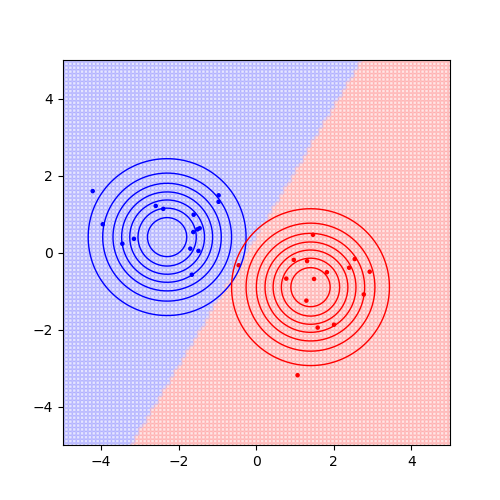
\includegraphics[scale=0.7]{img/GDA.png}
          \caption{GDA of Data Generated from 2 Gaussisans centered at $(-2.3, 0.4)$ and $(1.4, -0.9)$ with unit covariance. The decision boundary is slightly off since MLE approximates the true means. }
          \label{fig:gda}
      \end{figure}

  \subsection{Fisher Linear Discriminant} 

\section{Nonparametric Classification}

  \subsection{K Nearest Neighbors} 

    \begin{question}[To Do]
      Maybe similar like a kernel regression?  
    \end{question}

    Given a bunch of points in a metric space $(\mathcal{X}, d)$ that have classification labels, we want to label new datapoints $\hat{\mathbf{x}}$ based on the labels of other points that already exist in our dataset. One way to look at it is to look for close points within the dataset and use their labels to predict the new ones. 

    \begin{definition}[Closest Neighborhood]
      Given a dataset $\mathcal{D} = \{\mathbf{x}^{(i)}, \mathbf{y}^{(i)}\}$ and a point $\hat{\mathbf{x}} \in (\mathcal{X}, d)$, let the \textbf{k closest neighborhood} of $\hat{\mathbf{x}}$ be $N_k (\hat{\mathbf{x}}) \subset [N]$ defined as the indices $i$ of the $k$ points in $\mathcal{D}$ that is closest to $\hat{\mathbf{x}}$ with respect to the distance metric $d_\mathcal{X}$. 
    \end{definition}

    \begin{definition}[K Nearest Neighbors]
      The \textbf{K Nearest Neighbors (KNN)} is a discriminative nonparametric supervised learning algorithm that doesn't have a training phase. Given a new point $\hat{\mathbf{x}}$, we look at all points in its k closest neighborhood, and $h(\hat{\mathbf{x}})$ will be equal to whatever the majority class will be in. Let us one-hot encode the labels $\mathbf{y}^{(i)}$ into $\mathbf{e}_i$'s, and the number of data point in the $i$th class can be stored in the variable 
      \begin{equation}
        a_i = \sum_{i \in N_k (\hat{\mathbf{x}})} 1_{\{\mathbf{y}^{(i)} = \mathbf{e}_i\}}
      \end{equation}
      which results in the vector storing the counts of labels in the k closest neighborhood 
      \begin{equation}
        \mathbf{a} = (a_1, a_2, \ldots, a_\mathcal{K}) = \bigg( \sum_{i \in N_k (\hat{\mathbf{x}})} 1_{\{\mathbf{y}^{(i)} = \mathbf{e}_1\}}, \sum_{i \in N_k (\hat{\mathbf{x}})} 1_{\{\mathbf{y}^{(i)} = \mathbf{e}_2\}}, \ldots, \sum_{i \in N_k (\hat{\mathbf{x}})} 1_{\{\mathbf{y}^{(i)} = \mathbf{e}_\mathcal{K}\}} \bigg) 
      \end{equation}
      and take the class with the maximum element as our predicted label. 
    \end{definition}

    The best choice of $K$ depends on the data: 
    \begin{enumerate}
      \item Larger values of $K$ reduces the effect of noise on the classification, but make boundaries between classes less distinct. The number of misclassified data points (error) increases. 
      \item Smaller values are more sensitive to noise, but boundaries are more distinct and the number of misclassified data points (error) decreases.
    \end{enumerate}
    Too large of a $K$ value may increase the error too much and lead to less distinction in classification, while too small of a k value may result in us overclassifying the data. Finally, in binary (two class) classification problems, it is helpful to choose $K$ to be odd to avoid tied votes.

    This is an extremely simple algorithm that may not be robust. For example, consider $K \geq 3$, and we are trying to label a point $\hat{\mathbf{x}}$ that happens to be exactly where one point is on our dataset $\mathbf{x}^{(i)}$. Then, we should do $h(\hat{\mathbf{x}}) = y^{(i)}$, but this may not be the case if there are no other points with class $y^{(i)}$ in the k closest neighborhood of $\mathbf{x}^{(i)}$. Therefore, we want to take into account the distance of our new points from the others. 

    \begin{definition}[Weighted Nearest Neighbor Classifier]
      Let us define a monotinically decreasing function $\omega: \mathbb{R}_0^+ \mapsto \mathbb{R}_0^+$. Given a point $i \in N_k (\hat{\mathbf{x}})$, we can construct the weight of our matching label as inversely proportional to the distance: $\omega_i [ d(\hat{\mathbf{x}}, \mathbf{x}^{(i)})]$ and store them as 
      \begin{equation}
        \mathbf{a} = (a_1, a_2, \ldots, a_\mathcal{K}) = \bigg( \sum_{i \in N_k (\hat{\mathbf{x}})} \omega_i 1_{\{\mathbf{y}^{(i)} = \mathbf{e}_1\}}, \sum_{i \in N_k (\hat{\mathbf{x}})} \omega_i 1_{\{\mathbf{y}^{(i)} = \mathbf{e}_2\}}, \ldots, \sum_{i \in N_k (\hat{\mathbf{x}})} \omega_i 1_{\{\mathbf{y}^{(i)} = \mathbf{e}_\mathcal{K}\}} \bigg)
      \end{equation}
      and again take the class with the maximum element. 
    \end{definition}

    One caveat of KNN is in high dimensional spaces, as its performance degrades quite badly due to the curse of dimensionality. 

    \begin{example}[Curse of Dimensionality in KNN]
      Consider a dataset of $N$ samples uniformly distributed in a $d$-dimensional hypercube. Now given a point $x \in [0, 1]^d$, we want to derive the expected radius $r_k$ required to encompass its $k$ nearest neighbors. Let us define this ball to be $B_{r_k} \coloneqq \{ z \in \mathbb{R}^d \mid ||z - x ||_2 \leq r_k \}$. Since thse $N$ points are uniformly distributed, the expected number of points contained in $B_{r_k} (x)$ is simply the proportion of the volume that $B_{r_k} (x)$ encapsulates in the box, multiplied by $N$. Therefore, for some fixed $x$ and $r$, let us denote $Y(x, y)$ as the random variable representing the number of points contained within $B_r (x)$. By linearity of expectation and summing over the expectation for whether each point will be in the ball, we have 
      \[\mathbb{E}[Y (x, r)] = N \cdot \frac{\mu(B_r (x) \cap [0, 1]^d) }{\mu([0, 1]^d)}\]
      where $\mu$ is the Lebesgue measure of $\mathbb{R}^d$. Let us assume for not that we don't need to worry about cases where the ball is not fully contained within the cube, so we can just assume that $Y$ is only dependent on $r$: $Y(r)$. Also, since the volume of the hypercube is $1$,  $\mu([0, 1]^d) = 1$ and we get 
      \[\mathbb{E}[Y(r)] = N \cdot C_d \cdot r^d\]
      which we set equal to $k$ and evaluate for $r$. $C_d$ is a constant such that the volume of the hypersphere of radius $r$ can be derived as $V = C_d \cdot r^d$. We therefore get 
      \[N \cdot C_d \cdot r_k^d = k \implies r_k = \bigg( \frac{k}{N C_d} \bigg)^{1/d}\]
      It turns out that $C_d$ decreases exponentially, so the radius $r_k$ explodes as $d$ grows. Another way of looking at this is that in high dimensions, the $\ell_2$ distance between all the pairwise points are close in every single dimension, so it becomes harder to distinguish points that are close vs those that are far.  
    \end{example} 

    \subsubsection{Approximate K Nearest Neighbors}

  \subsection{Classification Trees}

    \begin{definition}[Decision Trees]
      Like K nearest neighbors, \textbf{decision trees} are discriminative nonparametric classification algorithms that involves creating some sort of tree that represents a set of decisions using a given set of input data $\mathbf{x}^{(i)}$ with its given classification $\mathbf{y}^{(i)}$. When predicting the class of a new input $\hat{\mathbf{x}}$, we would look at its attributes in some order, e.g. $\hat{x_1}, \hat{x}_2, \hat{x}_3$, and make a decision on which class it is in. 
      \begin{center}
          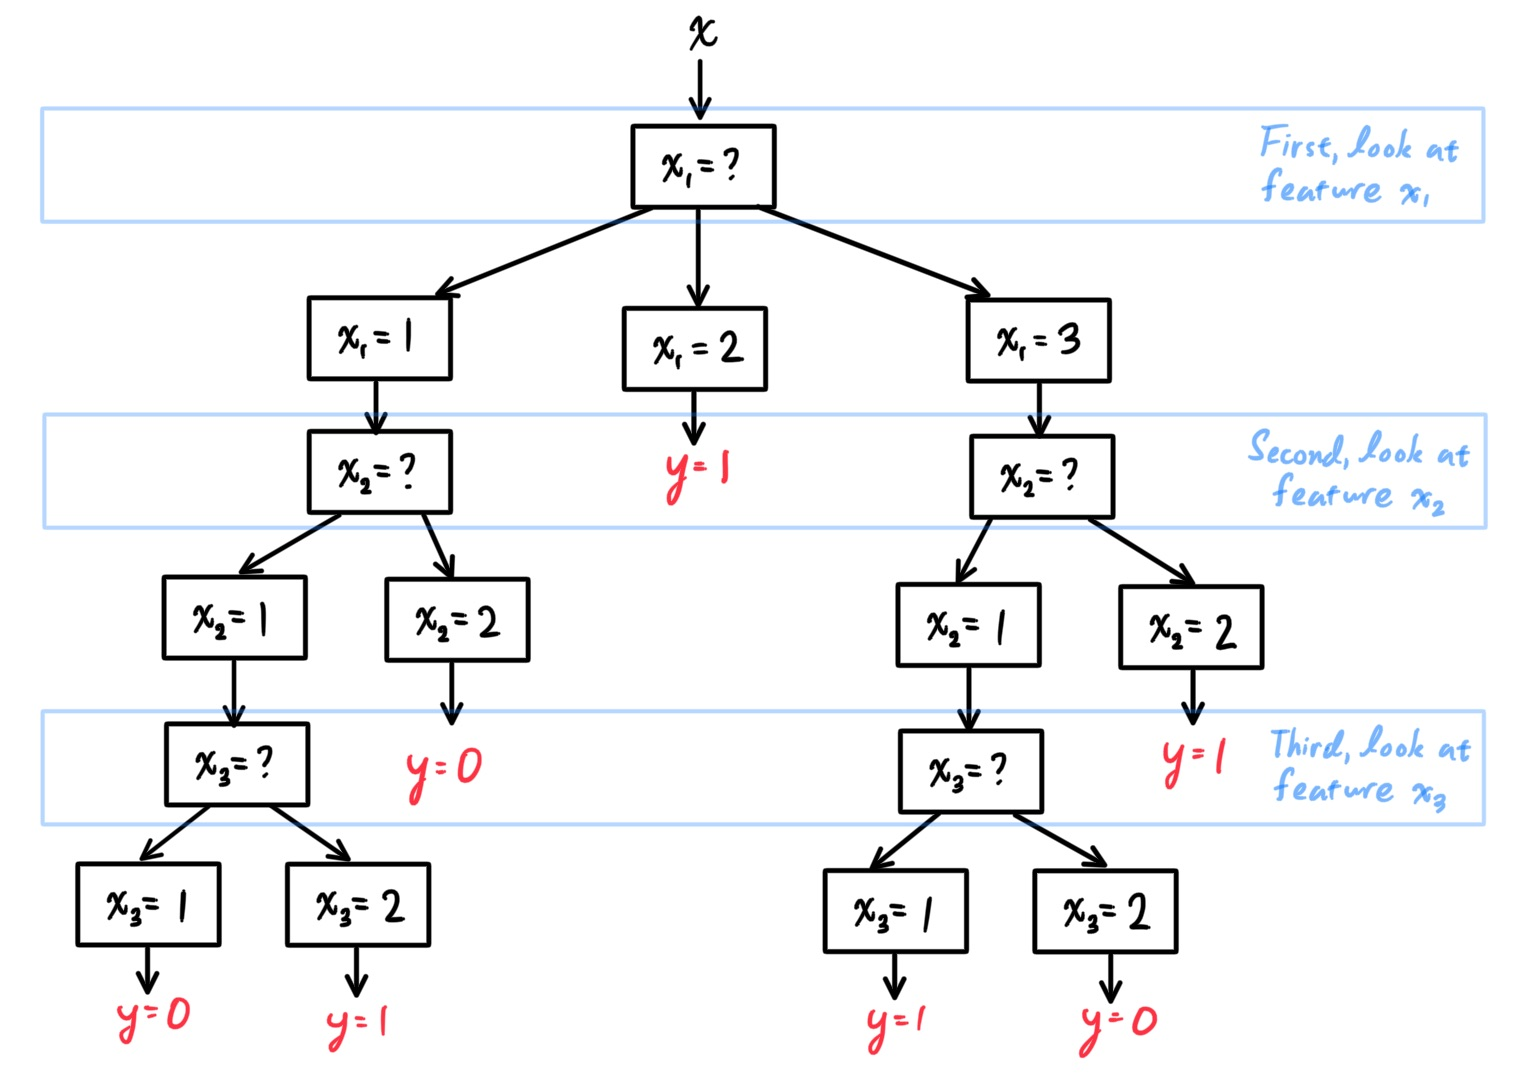
\includegraphics[scale=0.2]{img/general_decision_tree.jpg}
      \end{center}
      The decision tree tries to take advantage of some nontrivial covariance between $X$ and $Y$ by constructing nested partitions of the dataset $\mathcal{D}$, and within a partition, it predicts the label that comprises the majority. 
    \end{definition}

    For now, let us assume that $\mathcal{X}$ is a Cartesian product of discrete sets, and we will extend them to continuous values later. Let us look at an example to gain some intuition. 

    \begin{example}[Restaurant]
      Consider the dataset 
      \begin{center}
        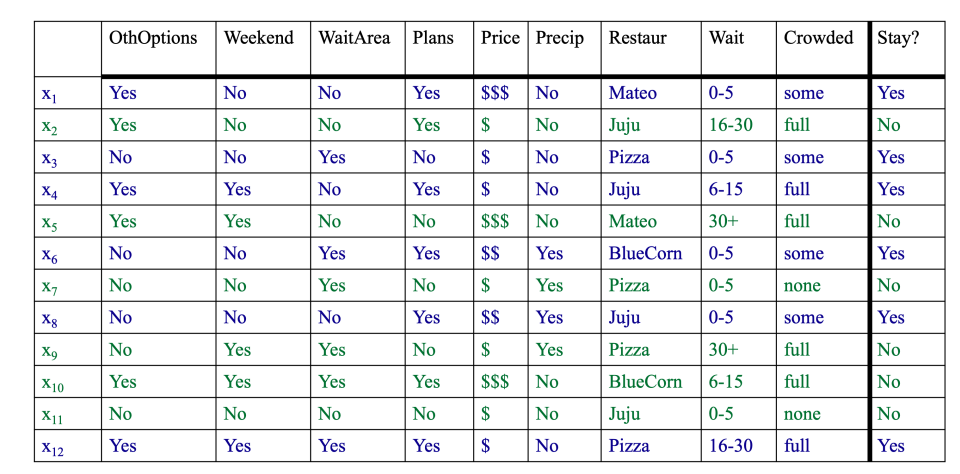
\includegraphics[scale=0.4]{img/decision_data.png}
      \end{center}
      Let us denote $\mathcal{D}$ as the dataset, and say that $F_1, \ldots, F_d$ were the features. This is a binary classification problem, and we can count that there are $6$ positives and $6$ negative labels. 
    \end{example}

    The simplest decision tree is the trivial tree, with one node that predicts the majority of the dataset. In this case, the data is evenly split, so without loss of generality we will choose $h_0 (\mathbf{x}) = 1$. We want to quantify how good our model is, and so like always we use a loss function. 

  

    Just like how a linear model is completely defined by its parameter $\boldsymbol{\theta}$, a decision tree is completely defined by the sequences of labels that it splits on. Therefore, training this is equivalent to defining the sequence, but we can't define this sequence unless we can compare how good a given decision tree is, i.e. unless we have defined a proper loss function. Depending on the training, we can use a greedy algorithm or not, and we have the flexibility to choose whether or not we can split on the same feature multiple times. 

    \begin{definition}[Misclassification Error]
      We will simply use the misclassification loss function. 
      \begin{equation}
        L(h; \mathcal{D}) = \frac{1}{N} \sum_{i=1}^N 1_{\{y^{(i)} \neq h(x^{(i)})\}} = 1 - \text{accuracy}
      \end{equation}
      Minimizing this maximizes the accuracy, so this is a reasonable one to choose. How do we train this? Unlike regression, this loss is not continuous, so the gradient is $0$, and furthermore the model isn't even parametric, so there are no gradients to derive! 
    \end{definition}

    Fortunately, the nature of the decision tree only requires us to look through the explanatory variables $x_1, \ldots, x_n$ and decide which one to split. 

    Let us take a decision tree $h$ and model the accuracy of it as a random variable: $1_{\{Y = h_0 (X)\}} \sim \mathrm{Bernoulli}(p)$, where $p$ is the accuracy. A higher accuracy of $h$ corresponds to a lower entropy, and so the entropy of the random variable is also a relevant indicator. 
    \[H(1_{\{Y = h_0 (X)\}}) = p \log{p} + (1 - p) \log(1 - p)\]
    Therefore, when we are building a tree, we want to choose the feature $x_i$ to split based on how much it lowers the entropy of the decision tree. 

    To set this up, let us take our dataset $\mathcal{D}$ and set $X_i$ as the random variable representing the distribution (a multinomial) of the $x_i^{(j)}$'s, and $Y$ as the same for the $y^{(j)}$'s. This is our maximum likelihood approximation for the marginalized distribution of the joint measure $X \times Y = X_1 \times \ldots \times X_D \times Y$. 

    Given a single node, we are simply going to label every point to be whatever the majority class is in $\mathcal{D}$. Therefore, we start off with the entropy of our trivial tree $H(Y)$. Then, we want to see which one of the $X_d$ features to split on, and so we can compute the conditional entropy $H(Y, X_d)$ to get the information gain $I(Y; X_d) = H(Y) - H(Y \mid X_d)$ for all $d = 1, \ldots, D$. We want to find a feature $X_d$ that maximize this information gain, i.e. decreases the entropy as much as possible (a greedy algorithm), and we find the next best feature (with or without replacement), so that we have a decreasing sequence. 
    \[H(X) \geq H(X ; Y) \geq H(X ; Y, Z) \geq H(X ; Y, Z, W) \geq \ldots \geq 0\]

    \begin{example}
      Continuing the example above, since there are $6$ labels of $0$ and $1$ each, we can model this $Y \sim \mathrm{Bernoulli}(0.5)$ random variable, with entropy 
      \[H(Y) = \mathbb{E}[-\log_2 p(Y)] = \frac{1}{2} \big( -\log_2 \frac{1}{2} \big) + \frac{1}{2} \big( -\log_2 \frac{1}{2} \big) = 1\]
      Now what would happen if we had branched according to how crowded it was, $X_{\mathrm{crowded}}$. Then, our decision tree would split into 3 sections: 
      \begin{center}
        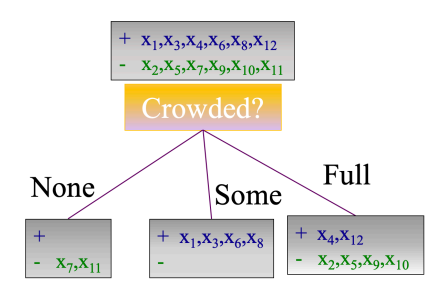
\includegraphics[scale=0.5]{img/decision_crowded.png}
      \end{center}
      In this case, we can define the multinomial distribution $X_{\mathrm{crowded}}$ representing the proportion of the data that is crowded in a specific level. That is, $X_{\mathrm{crowded}} \sim \mathrm{Multinomial}(\frac{2}{12}, \frac{4}{12}, \frac{6}{12} \big)$, with 
      \[\mathbb{P}(X_{\mathrm{crowded}} = x) = \begin{cases} 2/12 & \text{ if } x = \text{ none} \\ 4/12 & \text{ if } x = \text{ some} \\ 6/12 & \text{ if } x = \text{ full} \end{cases} \]
      Therefore, we can now compute the conditional entropy of this new decision tree conditioned on how crowded the store is 
      \begin{align*}
          H(Y \mid X_{\mathrm{crowded}}) & = \sum_x \mathbb{P}(X_{\mathrm{crowded}} = x) H(Y \mid X_{\mathrm{crowded}} = x) \\
          & = \frac{2}{12} H(\mathrm{Bern}(1)) + \frac{4}{12} H(\mathrm{Bern}(0)) + \frac{6}{12} H(\mathrm{Bern}(1/3)) = 0.459 \\
          I(Y; X_{\mathrm{crowded}}) & = 0.541
      \end{align*}
      We would do this for all the features and greedily choose the feature that maximizes our information gain. 
    \end{example}

    \begin{example}
      The Ferrari F1 team hired you as a new analyst! You were given the following table of the past race history of the team. You were asked to use information gain to build a decision tree to predict race wins. First, you will need to figure out which feature to split first. 

      \begin{center}
      \begin{tabular}[c]{c|c|c||c}
      Rain & Good Strategy & Qualifying & Win Race \\ \hline
      1 & 0 & 0 & 0 \\
      1 & 0 & 0 & 0 \\
      1 & 0 & 1 & 0 \\
      0 & 0 & 1 & 1 \\
      0 & 0 & 0 & 0 \\
      0 & 1 & 1 & 1 \\
      1 & 0 & 1 & 0 \\
      0 & 1 & 0 & 1 \\
      0 & 0 & 1 & 1 \\
      0 & 0 & 1 & 1 \\
      \end{tabular}
      \end{center}
      Let $X \sim \mathrm{Bernoulli}(1/2)$ be the distribution of whether a car wins a race over the data. Then its entropy is 
      \[H(X) = \mathbb{E}[-\log_2 p(x)] = \frac{1}{2} \big( -\log_2 \frac{1}{2} \big) + \frac{1}{2} \big( -\log_2 \frac{1}{2} \big) = 1\]
      Let $R \sim \mathrm{Bernoulli}(4/10), G \sim \mathrm{Bernoulli}(2/10), Q \sim \mathrm{Bernoulli}(6/10)$ be the distribution of the features rain, good strategy, and qualifying over the data, respectively. Then, the conditional entropy of $X$ conditioned on each of these random variables is 
      \begin{align*}
          H(X \mid R) & = \mathbb{P}(R = 1)\, H(X \mid R = 1) + \mathbb{P}(R = 0) \, H(X \mid R = 0) \\
          & = \frac{4}{10} \cdot - \big( 1 \cdot \log_2 1 + 0 \cdot \log_2 0 \big) + \frac{6}{10} \cdot - \big( \frac{1}{6} \cdot \log_2 \frac{1}{6} + \frac{5}{6} \cdot \log_2 \frac{5}{6} \big) \approx 0.390 \\
          H(X \mid G) & =  \mathbb{P}(G = 1)\, H(X \mid G = 1) + \mathbb{P}(G = 0) \, H(X \mid G = 0) \\
          & = \frac{2}{10} \cdot - \big( 1 \cdot \log_2 1 + 0 \cdot \log_2 0 \big) + \frac{8}{10} \cdot - \big( \frac{3}{8} \cdot \log_2 \frac{3}{8} + \frac{5}{8} \log_2 \frac{5}{8} \big) \approx 0.763\\
          H(X \mid Q ) & = \mathbb{P}(Q = 1)\, H(X \mid Q = 1) + \mathbb{P}(Q = 0) \, H(X \mid Q = 0) \\
          & = \frac{6}{10} \cdot - \big( \frac{4}{6} \cdot \log_2 \frac{4}{6} + \frac{2}{6} \cdot \log_2 \frac{2}{6} \big) + \frac{4}{10} \cdot - \big( \frac{1}{4} \log_2 \frac{1}{4} + \frac{3}{4} \log_2 \frac{3}{4} \big) \approx 0.875
      \end{align*}
      Therefore, the information gain are 
      \begin{align*}
          I(X; R) & = 1 - 0.390 = 0.610 \\
          I(X; G) & = 1 - 0.763 = 0.237 \\
          I(X; Q) & = 1 - 0.875 = 0.125 
      \end{align*}
      And so I would split on $R$, the rain, which gives the biggest information gain. 
    \end{example}

    Finally, we can use the Gini index of $X \sim \mathrm{Bernoulli}(p)$, defined 
    \begin{equation}
      G(X) = 2 p (1 - p)
    \end{equation}

    \begin{example}[Ferrari Example Continued]
      We do the same as the Ferrari example above but now with the Gini reduction. Let $X \sim \mathrm{Bernoulli}(1/2)$ be the distribution of whether a car wins a race over the data. Then its Gini index, which I will label with $\mathcal{G}$, is \[\mathcal{G} (X) = 2 \cdot \frac{1}{2} \cdot \frac{1}{2} = \frac{1}{2}\]
      Let $R \sim \mathrm{Bernoulli}(4/10), G \sim \mathrm{Bernoulli}(2/10), Q \sim \mathrm{Bernoulli}(6/10)$ be the distribution of the features rain, good strategy, and qualifying over the data, respectively. Then we compute the conditional expectation 
      \begin{align*}
          \mathbb{E}[\mathcal{G}(X \mid R)] & = \mathbb{P}(R = 1)\, \mathcal{G}(X \mid R = 1) + \mathbb{P}(R = 0) \, \mathcal{G}(X \mid R = 0) \\ 
          & = \frac{4}{10} \bigg[ 2 \cdot \frac{4}{4} \cdot \frac{0}{4} \bigg] + \frac{6}{10} \bigg[ 2 \cdot \frac{1}{6} \cdot \frac{5}{6} \bigg] \approx 0.167 \\
          \mathbb{E}[\mathcal{G}(X \mid G)] & = \mathbb{P}(G = 1)\, \mathcal{G}(X \mid G = 1) + \mathbb{P}(G = 0) \, \mathcal{G}(X \mid G = 0) \\ 
          & = \frac{2}{10} \bigg[ 2 \cdot \frac{2}{2} \cdot \frac{0}{2} \bigg] + \frac{8}{10} \bigg[ 2 \cdot \frac{3}{8} \cdot \frac{5}{8} \bigg] \approx 0.375 \\
          \mathbb{E}[\mathcal{G}(X \mid Q)] & = \mathbb{P}(Q = 1)\, \mathcal{G}(X \mid Q = 1) + \mathbb{P}(Q = 0) \, \mathcal{G}(X \mid Q = 0) \\ 
          & = \frac{6}{10} \bigg[ 2 \cdot \frac{4}{6} \cdot \frac{2}{6} \bigg] + \frac{4}{10} \bigg[ 2 \cdot \frac{1}{4} \cdot \frac{3}{4} \bigg] \approx 0.417
      \end{align*}
      Therefore, the Gini reduction, which I'll denote as $I_{\mathcal{G}}$, is 
      \begin{align*}
          I_{\mathcal{G}} (X ; R) & = 0.5 - 0.167 = 0.333 \\
          I_{\mathcal{G}} (X ; G) & = 0.5 - 0.375 = 0.125 \\
          I_{\mathcal{G}} (X ; Q) & = 0.5 - 0.417 = 0.083
      \end{align*}
      Since branching across the feature $R$, the rain, gives the biggest Gini reduction, we want to split on the rain feature first. 
    \end{example}

    \subsubsection{Regularization}

      Given a dataset with $D$ binary features, let $g(H, D)$ be the number of binary trees with depth at most $H$ (including root node), with the restriction that the trees may not split on some variable multiple times within a path to a leaf node. Then, $g$ can be defined recursively. 
      \begin{enumerate}
          \item First, if $H = 1$, then $g(H, D) = 1$ always since we are just creating the trivial binary tree of one node. 
          \item If $D = 0$, then there are no features to split on and therefore we just have the single node $g(H, D) = 1$. 
          \item If $H > 1$ and $D > 0$, then say that we start with a node. We can either make this a leaf node by not performing any splitting at all, or split on one of the $D$ variables. Then for each of the 2 nodes created on the split, we are now working with $D-1$ features and a maximum height of $H-1$ for each of the subtrees generated from the 2 nodes. 
      \end{enumerate}
      All this can be expressed as 
      \[g(H, D) = \begin{cases} 1 + D \, \big[ g(H - 1, D - 1) \big]^2 & \text{ if } H > 1, D > 0 \\ 1 & \text{ if } H = 1 \text{ or } D = 0 \end{cases} \]
      which is extremely large (in fact, NP hard). Therefore, some tricks like regularization must be implemented to limit our search space. 

      By defining the complexity of our decision tree $\Omega(h)$ as the number of nodes within the tree, we can modify our objective function to 
      \[L(h; \mathcal{D}) = \frac{1}{N} \sum_{i=1}^N 1_{\{y^{(i)} \neq h(x^{(i)})\}} + \lambda \Omega(h)\]
      We can impose this constraint directly on the training algorithm, or we can calculate the regularized loss after the tree has been constructed, which is a method called \textbf{tree pruning}. 

      Given a large enough $\lambda$, we can in fact greatly reduce our search space by not considering any trees further than a certain point. 

      \begin{theorem}
      We describe a tree as a set of leaves, where leaf $k$ is a tuple containing the logical preposition satisfied by the path to leaf $k$, denoted $p_k $, and the class label predicted by the leaf, denoted $\hat{y}_k$. For a dataset with $d$ binary features, $p_k: \{0, 1\}^d \to \{0, 1\}$ is a function that returns $1$ if a sample $x_i$ satisfies the preposition, and $0$ otherwise. That is, leaf $k$ is $(p_k, \hat{y}_k),$ and a tree $f$ with $K$ leaves is described as a set $f = \{(p_1, \hat{y}_1), \hdots, (p_K, \hat{y}_K)\}$. Assume that the label predicted by $\hat{y}_k$ is always the label for the majority of samples satisfying $p_k$. Finally, let $m_k = \sum_{i=1}^n p_k(x_i)$ denote the number of training samples ``captured'' by leaf $k$.

      Given a (potentially optimal) tree 

        \[f = \{(p_1, \hat{y}_1), \hdots, (p_{\kappa}, \hat{y}_{\kappa}), \hdots, (p_K, \hat{y}_K)\}, \]

      the tree $f' = \{(p_1, \hat{y}_1), \hdots, (p_{\kappa_1}, \hat{y}_{\kappa_1}), (p_{\kappa_2}, \hat{y}_{\kappa_2}), \hdots, (p_K, \hat{y}_K)\}$ produced by splitting leaf $(p_{\kappa}, \hat{y}_{\kappa})$ into two leaves $(p_{\kappa_1}, \hat{y}_{\kappa_1})$ and $(p_{\kappa_2}, \hat{y}_{\kappa_2})$ and any tree produced by further splitting $(p_{\kappa_1}, \hat{y}_{\kappa_1})$ or $(p_{\kappa_2}, \hat{y}_{\kappa_2})$ cannot  be optimal if $m_{\kappa} < 2n\lambda$.
      \end{theorem}
      \begin{proof}
      Let $c$ be the number of misclassifications in leaf $(p_{\kappa}, \hat{y}_{\kappa})$. Since a leaf classifies according to the majority of $m_{\kappa}$, we must have 

        \[c \leq \frac{m_\kappa}{2} < n \lambda\]

      By splitting leaf $(p_\kappa, \hat{y}_\kappa)$ into leaves $(p_{\kappa_1}, \hat{y}_{\kappa_1})$ and $(p_{\kappa_2}, \hat{y}_{\kappa_2})$, assume that we have reduced the number of misclassifications by $b \leq c$. Then, we have 

        \[\ell(f^\prime, \mathbf{X}, \mathbf{y}) = \ell(f, \mathbf{X}, \mathbf{y}) - \frac{b}{n}\]

      However, we have increased the number of leaves by $1$, and so 

        \[\lambda s(f^\prime) = \lambda s(f) + \lambda\]

      Combining the last two equations, we have obtained 

        \[R (f^\prime, \mathbf{X}, \mathbf{y}) = R(f, \mathbf{X}, \mathbf{y}) + \lambda - \frac{b}{n}\]

      However, we know that 

      \begin{align*}
        b \leq c & \implies \frac{b}{n} \leq \frac{c}{n} < \frac{n \lambda}{n} = \lambda \\
        & \implies - \frac{b}{n} > - \lambda \\
        & \implies \lambda - \frac{b}{n} > \lambda - \lambda = 0
      \end{align*}

      and so $R (f^\prime, \mathbf{X}, \mathbf{y}) > R(f, \mathbf{X}, \mathbf{y})$. This means that $f^\prime$ cannot be optimal according to our regularized objective. We have also proved that further splitting $(p_{\kappa_1}, \hat{y}_{\kappa_1})$ or $(p_{\kappa_2}, \hat{y}_{\kappa_2})$ cannot  be optimal since we can just set $f = f^\prime$, and apply the same argument. 
      \end{proof}

\section{Generalized Linear Models} 

  Remember the linear model looked like this, where we use the conventional $\beta$ notation to represent parameters. 
  \begin{equation}
    Y = X^T \beta + \epsilon, \;\; \epsilon \sim N(0, \sigma^2 I)
  \end{equation}
  which implies that $Y \mid X \sim N(X^T \beta, \sigma^2 I)$. Basically, given $x$, I assume some distribution of $Y$, and the value of $x$ will help me guess what the mean of this distribution is. Note that we in here assume that only the mean depends on $X$. I could potentially have something crazy, like 
  \[Y \mid X \sim N(X^T \beta, (X^T \gamma) (X X^T + I))\]
  where the covariance will depend on $X$, too, but in this case we only assume that that mean is dependent on $X$. 
  \[Y \mid X \sim N(\mu(X), \sigma^2 I)\]
  where in the linear model, $\mu(X) = X^T \beta$. So, there are three assumptions we are making here: 
  \begin{enumerate}
    \item $Y \mid X$ is Gaussian. 
    \item $X$ only affects the mean of $Y \mid X$, written $\mathbb{E}[Y \mid X] = \mu(X)$. 
    \item $X$ affects the mean in a linear way, such that $\mu(X) = X^T \beta$. 
  \end{enumerate}
  So the two things we are trying to relax are: 
  \begin{enumerate}
    \item \textbf{Random Component}: the response variable $Y \mid X$ is continuous and normally distributed with mean $\mu = \mu(X) = \mathbb{E}[Y \mid X]$. 
    \item \textbf{Link}: I have a link that explains the relationship between the $X$ and the $\mu$, and this relationship is $\mu(X) = X^T \beta$. 
  \end{enumerate}
  So when talking about GLMs, we are not changing the fact that we have a linear function $X \mapsto X^T \beta$. However, we are going to assume that $Y \mid X$ now comes from a broader \textbf{family of exponential distributions}. Second, we are going to assume that there exists some \textbf{link function} $g$
  \[g(\mu(X)) = X^T \beta\]
  Admittedly, this is not the most intuitive way to think about it, since we would like to have $\mu(X) = f(X^T \beta)$, but here we just decide to call $f = g^{-1}$. Therefore, if I want to give you a GLM, I just need to give you two things: the conditional distribution $Y \mid X$, which can be any distribution in the exponential family, and the link function $g$. 

  We really only need this link function due to compatibility reasons. Say that $Y \mid X \sim \mathrm{Bern}(p)$. Then, $\mu(X) = \mathbb{E}[Y \mid X]$ always lives in $[0, 1]$, but $X^T \beta$ always lives in $\mathbb{R}$. We want our model to be realistic, and we can clearly see the problem shown in Figure \ref{fig:Bernoulli_GLM}. 

  \begin{figure}[H]
    \centering
    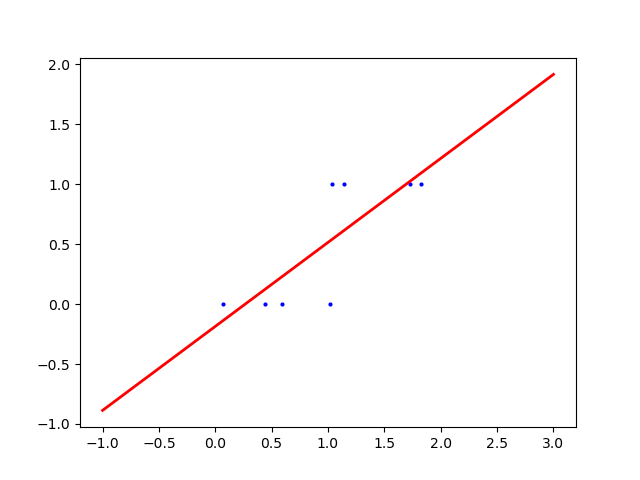
\includegraphics[scale=0.5]{img/GLM_bernoulli.png}
    \caption{Fitting a linear model for Bernoulli random variables will predict a mean that is outside of $[0, 1]$ when getting new datapoints. }
    \label{fig:Bernoulli_GLM}
  \end{figure}

  If $Y \mid X$ is some exponential distribution, then its support is always positive and so $\mu(X) > 0$. But if we stick to the old form of $\mu(X) = X^T \beta$, then $\mathrm{Im}(\mu) = \mathbb{R}$, which is not realistic when we predict negative values. Let's take a couple examples: 

  \begin{example}[Disease Epidemic]
    In the early stages of a disease epidemic, the rate at which new cases occur can often increase exponentially through time. Clearly, $\mu(X) = \mathbb{E}[Y \mid X]$ should be positive and we should have some sort of exponential trend. Hence, if $\mu(x)$ is the expected number of cases on data $x$, a model of the form 
    \begin{equation}
      \mu(x) = \gamma \exp (\delta x)
    \end{equation}
    seems appropriate, where $\gamma$ and $\delta$ are simply scaling factors. Clearly, $\mu(X)$ is not of the form $f(X^T \beta)$. So what I do is to transform $\mu$ in such a way that I can get something that is linear. 
    \begin{equation}
      \log(\mu(X)) = \log(\gamma) + \delta X
    \end{equation}
    which is now linear in $X$, of form $\beta_0 + \beta_1 X$. This will have some effects, but this is what needs to be done to have a genearlized linear model. Note that what I did to $\mu$ was take the log of it, and so the link function is $g = \log$, called the \textbf{log-link}. Now that we have chosen the $g$, we still need to choose what the conditional distribution $Y \mid X$ would be. This is determined by speaking with industry professionals, experience, and convenience. In this case, $Y$ is a count, and since this must be a discrete distribution. Since it is not bounded above, we think Poisson. 
  \end{example}

  \begin{example}[Prey Capture Rate]
    The rate of capture of preys, $Y$, by a hunting animal, tends to increase with increasing density of prey $X$, but eventually level off when the predator is catching as much as it can cope with. We want to find a perhaps concave function that levels off, and suitable model might be 
    \begin{equation}
      \mu(X) = \frac{\alpha X}{h + X}
    \end{equation}
    where $\alpha$ represents the maximum capture rate, and $h$ represents the prey density at which the capture rate is half the maximum rate. Again, we must find some transformation $g$ that turns this into a linear function of $X$, and what we can do it use the \textbf{reciprocal-link}. 
    \begin{equation}
      \frac{1}{\mu(X)} = \frac{h + X}{\alpha X} = \frac{h}{\alpha} \frac{1}{X} + \frac{1}{\alpha}
    \end{equation}
    The standard deviation of capture rate might be approximately proportional to the mean rate, suggesting the use of a Gamma distribution for the response. 
  \end{example}

  \begin{example}[Kyphosis Data]
    The Kyphosis data consist of measurements on $81$ children following corrective spinal surgery. The binary response variable, Kyphosis, indicates the presence or absence of a postoperative deforming. The three covariates are: age of the child in months, number of the vertebrae involved in the operation, and the start of the range of the vertebrae involved. The response variable is binary so there is no choice: $Y \mid X$ is Bernoulli with expected value $\mu(X) \in (0, 1)$. We cannot write $\mu(X) = X^T \beta$ because the right hand side ranges through $\mathbb{R}$, and so we find an invertible function that squishes $\mathbb{R}$ to $(0, 1)$, and so we can choose basically any CDF. 
  \end{example}

  For clarification, when writing a distribution like $\mathrm{Bernoulli}(p)$, or $\mathrm{Binomial}(n, p)$, $\mathrm{Poisson}(\lambda)$, or $N(\mu, \sigma^2)$, the hyperparameters that we usually work with we will denote as $\boldsymbol{\theta}$, and the space that this $\boldsymbol{\theta}$ lives in will denote $\Theta$. For example, for the Bernoulli, $\Theta = [0, 1]$, and for Poisson, $\Theta = [0, +\infty)$. 

  Ultimately, a GLM consists of three steps: 
  \begin{enumerate}
    \item The observed input $X$ enters the model through a linear function $\beta^T X$. 
    \item The conditional mean of response, is represented as a function of the linear combination 
      \begin{equation}
        \mathbb{E}[Y \mid X] = \mu = f(\beta^T X)
      \end{equation}
    \item The observed response is drawn from an exponential family distribution with conditional mean $\mu$. 
  \end{enumerate}

  \subsection{Exponential Family}

    We can write the pdf of a distribution as a function of the input $x$ and the hyperparameters $\theta$, so we can write $P_\theta (x) = p(\theta, x)$. For now, let's think that both $x, \theta \in \mathbb{R}$. Think of all the functions that depend on $\theta$ and $x$. There are many of them, but we want $\theta$ and $x$ to interact in a certain way. The way that I want them to interact with each other is that they are multiplied within an exponential term. Now clearly, this is not a very rich family, so we are just slapping some terms that depend only on $\theta$ and only on $x$. 
    \[p_\theta (x) = \exp(\theta x) h(x) c(\theta)\]
    But now if $\theta \in \mathbb{R}^k$ and $x \in \mathbb{R}^q$, then we cannot simply take the product nor the inner product, but what we can do is map both of them into a space that has the same dimensions, so I can take the inner product. That is, let us map $\boldsymbol{\theta} \mapsto \boldsymbol{\eta}(\boldsymbol{\theta}) \in \mathbb{R}^k$ and $\mathbf{x} \mapsto \mathbf{T}(\mathbf{x}) \in \mathbb{R}^k$, and so 
    our exponential distribution form would be generalized into something like 
    \[p_{\boldsymbol{\theta}} (\mathbf{x}) = \exp\big[ \boldsymbol{\eta}(\boldsymbol{\theta}) \cdot \mathbf{T}(\mathbf{x}) \big] h(\mathbf{x}) c(\boldsymbol{\theta})\]
    We can think of $c(\boldsymbol{\theta})$ as the normalizing term that allows us to integrate the pdf to $1$. 
    \[\int_\mathcal{X} p_{\boldsymbol{\theta}} (\mathbf{x}) = c(\boldsymbol{\theta}) \int \exp\big[\boldsymbol{\eta}(\boldsymbol{\theta}) \cdot \mathbf{T}(\mathbf{x}) \big] h(\mathbf{x})  \,d\mathbf{x}\]
    We can just push the $c(\boldsymbol{\theta})$ term into the exponential by letting $c(\boldsymbol{\theta}) = e^{-\log(c(\boldsymbol{\theta}))^{-1}}$ to get our definition. 

    \begin{definition}[Exponential Family]
      A \textbf{k-parameter exponential family} is a family of distributions with pdf/pmf of the form 
      \[p_{\boldsymbol{\theta}} (\mathbf{x}) = \exp\big[ \boldsymbol{\eta}(\boldsymbol{\theta}) \cdot \mathbf{T}(\mathbf{x}) - B(\boldsymbol{\theta}) \big] h(\mathbf{x})\]
      The $h$ term, as we will see, will not matter in our maximum likelihood estimation, so we keep it outside the exponential. 
      \begin{enumerate}
        \item $\boldsymbol{\eta}$ is called the \textbf{canonical parameter}. Given a distribution parameterized by the regular hyperparameters $\boldsymbol{\theta}$, we would like to parameterize it in a different way $\boldsymbol{\eta}$ under the function $\boldsymbol{\eta}: \Theta \rightarrow \mathbb{R}$
        \item $\mathbf{T}(\mathbf{x})$ is called the \textbf{sufficient statistic}. 
        \item $h(\mathbf{x})$ is a nonnegative scalar function. 
        \item $B(\boldsymbol{\theta})$ is the normalizing factor. 
      \end{enumerate}
    \end{definition}

    Let's look at some examples. 

    \begin{example}[Gaussian]
      If we put the coefficient into the exponential and expand the square term, we get 
      \[p_\theta (x) = \exp \bigg( \frac{\mu}{\sigma^2} \cdot x - \frac{1}{2\sigma^2} \cdot x^2 - \frac{\mu^2}{2 \sigma^2} - \log ( \sigma \sqrt{2 \pi}) \bigg)\] 
      where 
      \[\boldsymbol{\eta}(\boldsymbol{\theta}) = \begin{pmatrix} \mu /\sigma^2 \\ -1 / 2 \sigma^2 \end{pmatrix}, \; T(x) = \begin{pmatrix} x \\ x^2 \end{pmatrix}, \; B(\theta) = \frac{\mu^2}{2 \sigma^2} + \log(\sigma \sqrt{2 \pi}), \; h(x) = 1\]
      This is not a unique representation since we can take the $\log(\sqrt{2 \pi})$ out of the exponential, but why bother to do this when we can just stuff everything into $B$ and keep $h$ simple. 
    \end{example}

    \begin{example}[Gaussian with Known Variance]
      If we have known variance, we can write the Gaussian pdf as 
      \[p_\theta (x) = \exp \bigg[ \frac{\mu}{\sigma} \cdot \frac{x}{\sigma} - \frac{\mu^2}{2 \sigma^2} \bigg] \cdot \frac{1}{\sigma \sqrt{2\pi}} e^{x^2/2 \sigma^2}\]
      where 
      \[\eta(\theta) = \frac{\mu}{\sigma}, \; T(x) = \frac{x}{\sigma}, \; B(\theta) = \frac{\mu^2}{2 \sigma^2}, \; h(x) = \frac{1}{\sigma \sqrt{2 \pi}} e^{x^2/2 \sigma^2}\]
    \end{example}

    \begin{example}[Bernoulli]
    The pmf of a Bernoulli with $\theta$ is 
    \begin{align*}
        p_\theta (x) & = \theta^x (1 - \theta)^{(1 - x)} \\
        & = \exp \big[x \log (\theta) + (1 - x)\log(1 - \theta) \big] \\
        & = \exp \bigg( x \log \Big[ \frac{\theta}{1 - \theta} \Big] - \log \Big[ \frac{1}{1 - \theta} \Big] \bigg)
    \end{align*}
    where 
    \[\eta(\theta) = \log \Big[ \frac{\theta}{1 - \theta} \Big], \; T(x) = x, \; B(\theta) = \log \Big[ \frac{1}{1 - \theta} \Big], \; h(x) = 1\]
    \end{example}


    \begin{example}[Binomial with Known Number of Trials]
    We can transform a binomial with known $N$ as 
    \begin{align*}
      p_\theta (x) &  = \binom{N}{x} \theta^x  (1 - \theta)^{1 - x} \\
                   & = \exp \bigg[ x \ln \big( \frac{\theta}{1 - \theta} \Big) + \ln(1 - \theta) \bigg] \cdot \binom{N}{x} 
    \end{align*}
    where 
      \[\eta (\theta) = \ln \big( \frac{\theta}{1 - \theta} \Big), \; T(x) = x, \; B(\theta) = \ln(1 - \theta), \; h(x) = \binom{N}{x}\]
    \end{example}

    \begin{example}[Poisson]
    The pmf of Poisson with $\theta$ can be expanded 
    \begin{align*}
        p_\theta & = \frac{\theta^{-x}}{x!} e^{-\theta} \\
        & = \exp \big[ -\theta + x\log(\theta) - \log(x!) \big] \\
        & = \exp \big[ x \log(\theta) - \theta \big] \, \frac{1}{x!}
    \end{align*}
    where 
    \[\eta(\theta) = \log(\theta), \; T(x) = x, \; B(\theta) = \theta, \; h(x) = \frac{1}{x!}\]
    \end{example}

    However, the uniform is not in here. In fact, any distribution that has a support that does not depend on the parameter is not an exponential distribution. 

    Let us now focus on one parameter families where $\theta \in \Theta \subset \mathbb{R}$, which do not include the Gaussian (with unknown mean and variance, Gamma, multinomial, etc.), which has a pdf written in the form 
    \[p_\theta (x) = \exp \big[ \eta (\theta) \, T(x) - B(\theta) \big] \, h(x)\]


    \subsubsection{Canonical Exponential Family}

      Now a common strategy in statistical analysis is to reparamaterize a probability distribution. Suppose a family of probability distributions $\{P_\theta\}$ is parameterized by $\theta \in \Theta \subset \mathbb{R}$. If we have an invertible function $\eta: \Theta \rightarrow \mathcal{T} \subset \mathbb{R}$, then we can paramaterize the same family with $\eta$ rather than $\theta$, with no loss of information. Typically, it is the case that $\eta$ is invertible for exponential families, so we can just reparameterize the whole pdf and write 
      \[p_\eta (x) = \exp \big[ \eta \, T(x) - \phi(\eta) \big] \, h(x)\]
      where $\phi = B \circ \eta^{-1}$. 

      \begin{definition}[Canonical One-Parameter Exponential Family]
      A family of distributions is said to be in \textbf{canonical one-parameter exponential family} if its density is of form 
      \[p_\eta (x) = \exp \big[ \eta \, T(x) - \phi(\eta) \big] \, h(x)\]
      which is a subfamily of the exponential family. The function $\psi$ is called the \textbf{cumulant generating function}. 
      \end{definition}

      Before we move on, let us just provide a few examples. 

      \begin{example}[Poisson]
      The Poisson can be represented as 
      \[p_\theta (x) = \exp \big[ x \log{\theta} - \theta \big] \, \frac{1}{x!}\]
      Now let $\eta = \log{\theta} \implies \theta = e^{\eta}$. So, we can reparamaterize the density as 
      \[p_\eta(x) = \exp \big[ x \eta - e^\eta \big] \, \frac{1}{x!}\]
      where $P_\eta = \mathrm{Poisson}(e^\eta)$ for $\eta \in \mathcal{T} = \mathbb{R}$, compared to $P_\theta = \mathrm{Poisson}(\theta)$ for $\theta \in \Theta = \mathbb{R}^+$. 
      \end{example}

      \begin{example}[Gaussian]
      Recall that the Gaussian with known parameter $\sigma^2$ and unknown $\theta = \mu$ is in the exponential family, since we can expand it as 
      \[p_\theta (x) = \exp \bigg[ \frac{\mu}{\sigma^2} \cdot x - \frac{\mu^2}{2 \sigma^2} \bigg] \cdot \frac{1}{\sigma \sqrt{2\pi}} e^{x^2/2 \sigma^2}\]
      We can perform the change of parameter $\eta = \mu^2 / 2\sigma^2 \implies \mu = \sigma^2 \eta$, and substituting this in will give the canonical representation 
      \[p_\eta (x) = \exp \Big[ \eta x - \frac{\sigma^2 \eta^2}{2} \Big] \cdot \frac{1}{\sigma \sqrt{2\pi}} e^{x^2/2 \sigma^2}\]
      where now $P_\eta = N(\sigma^2 \eta, \sigma^2)$ for $\eta \in \mathcal{T} = \mathbb{R}$, compared to $P_\theta = N(\theta, \sigma^2)$ for $\theta \in \Theta = \mathbb{R}$, which is basically the same space. 
      \end{example}

      \begin{example}[Bernoulli]
      The Bernoulli has an exponential form of 
      \[p_\theta (x) = \exp \bigg[ x \log \Big( \frac{\theta}{1 - \theta} \Big) + \log(1 - \theta)\bigg]\]
      Now setting $\eta = \log\big( \frac{\theta}{1 - \theta} \big) \implies \theta = \frac{1}{1 + e^{-\eta}}$, and so $B(\theta) = - \log(1 - \theta) = - \log \big( \frac{e^{-\eta}}{1 + e^{-\eta}} \big) = \log(1 + e^\eta) = \psi(\eta)$, and so the canonical paramaterization is 
      \[p_\eta (x) = \exp \big[ x \eta - \log(1 + e^{\eta}) \big]\]
      \end{example}


      We present two useful properties of the exponential family. 

      \begin{theorem}[Moments]
      Let random variable $X$ be in the canonical exponential family $P_\eta$ 
      \[p_\eta (x) = e^{\eta T(x) - \psi(\eta)} h(x)\]
      Then, the expectation and variance are encoded in the cumulant generating function in the following way 
      \[\mathbb{E} [T(X)] = \psi^\prime (\eta) \;\;\;\;\;\;\;\; \Var[T(X)] = \psi^{\prime\prime} (\eta)\]
      \end{theorem}
      \begin{proof}

      \end{proof}

      \begin{example}
      We show that this is consistent with the Poisson, normal, and Bernoulli distributions. 
      \begin{enumerate}
          \item In the Poisson, $\psi(\eta) = e^{\eta}$, and so $\psi^\prime(\eta) = e^\eta = \theta = \mathbb{E}[X]$. Taking the second derivative gives $\psi^{\prime\prime}(\eta) = e^\eta = \theta = \Var[X]$, too. \
          
          \item In the Normal with known variance $\sigma^2$, we have $\psi(\eta) = \frac{1}{2} \sigma^2 \eta^2$. So 
          \begin{align*}
              \mathbb{E}[X] & = \psi^\prime (\eta) = \sigma^2 \eta = \mu \\
              \Var[X] & = \psi^{\prime\prime} (\eta) = \sigma^2
          \end{align*}

          \item In the Bernoulli, we have $\psi(\eta) = \log(1 + e^{-\eta})$. Therefore, 
          \begin{align*}
              \mathbb{E}[X] & = \psi^\prime (\eta) = \frac{x^\eta}{1 + x^{\eta}} = \frac{1}{1 + e^{-\eta}} = \theta \\
              \Var[X] & = \psi^{\prime\prime} (\eta) = -\bigg(\frac{1}{1 + e^{-\eta}}\bigg)^2 \, e^{-\eta} \cdot -1 = \theta^2 \cdot \frac{1 - \theta}{\theta} = \theta (1 - \theta) 
          \end{align*}
      \end{enumerate}
      \end{example}

      \begin{theorem}[Convexity]
      Consider a canonical exponential family with density 
      \[p_\eta (x) = e^{\eta T(x) - \psi(\eta)} h(x)\]
      and natural parameter space $\mathcal{T}$. Then, the set $\mathcal{T}$ is convex, and the cumulant generating function $\psi$ is convex on $\mathcal{T}$. 
      \end{theorem}
      \begin{proof}
      This can be proven using Holder's inequality. However, from the theorem above, note that $\Var[T(X)] = \psi^{\prime\prime}(\eta)$ must be positive since we are talking about variance. This implies that the second derivative of $\psi$ is positive, and therefore must be convex. 
      \end{proof}

      We will look at a subfamily of the exponential family. Now remember that we introduce the functions $\boldsymbol{\eta}$ and $\mathbf{T}$ so that we can capture a much broader range of distributions, but if we have one parameter $k = 1$, then we can just set $\boldsymbol{\eta}(\boldsymbol{\theta})$ to be the new parameter $\theta$. The \textbf{canonical exponential family} for $k = 1, y \in \mathbb{R}$, is defined to have the pdf 
      \begin{equation}
        f_\theta (y) = \exp \bigg( \frac{y \theta - b(\theta)}{\phi} + c(y, \phi) \bigg)
      \end{equation}
      where 
      \begin{equation}
        h(y) = \exp \big( c(y, \phi)\big)
      \end{equation}
      If $\phi$ is known, this is a one-parameter exponential family with $\theta$ being the \textbf{canonical parameter}, and if $\phi$ is unknown, the $h(y)$ term will not depend on $\theta$, which we may not be able to split up into the exponential pdf form. In this case $\phi$ is called the \textbf{dispersion parameter}. For now, we will always assume that $\phi$ is known. 

      We can prove this for all other classes, too. We can think of the $c(y, \phi)$ as just a term that we stuff every other term into. What really differentiates the different distributions of the canonical exponential family is the $b(\theta)$. The form of $b$ will determine whether this distribution is a Gaussian, or a Bernoulli, or etc. This $b$ will capture information about the mean, the variance, the likelihood, about everything. 

      \subsection{Cumulant Generating Function}

        \begin{definition}[Score]
        The \textbf{score} is the gradient of the log-likelihood function with respect to the parameter vector. That is, given that $L(\boldsymbol{\theta})$ is the likelihood, then 
        \[s(\boldsymbol{\theta}) \coloneqq \frac{\partial \log L(\boldsymbol{\theta}; \mathbf{x})}{\partial \boldsymbol{\theta}}\]
        which gives a row covector. 
        \end{definition}

        Now, remember that the score also depends on the observations $\mathbf{x}$. If we rewrite the likelihood as a probability density function $L(\boldsymbol{\theta}; \mathbf{x}) = f(\mathbf{x}; \boldsymbol{\theta})$, then we can say that the expected value of the score is equal to $0$, since 
        \begin{align*}
         \mathbb{E}[s(\boldsymbol{\theta})] & = \int_\mathcal{X} f(\mathbf{x}; \boldsymbol{\theta}) \frac{\partial}{\partial \boldsymbol{\theta}} \log L (\boldsymbol{\theta}; \mathbf{x}) \,d\mathbf{x} \\
         & = \int_\mathcal{X} f(\mathbf{x}; \boldsymbol{\theta}) \frac{1}{f(\mathbf{x}; \boldsymbol{\theta})} \, \frac{\partial f(\mathbf{x}; \boldsymbol{\theta})}{\partial \boldsymbol{\theta}} \,dx \\
         & = \frac{\partial}{\partial \boldsymbol{\theta}} \int_\mathcal{X} f(\mathbf{x}; \boldsymbol{\theta}) \,d \mathbf{x} \\
         & = \frac{\partial}{\partial \boldsymbol{\theta}} 1 = 0
        \end{align*}
        where we take a leap of faith in switching the derivative and integral in the penultimate line. Furthermore, we can get the second identity 
        \[\mathbb{E}\bigg[ \frac{\partial^2 \ell}{\partial \theta^2} \bigg] + \mathbb{E} \bigg[ \frac{\partial \ell}{\partial \theta} \bigg]^2 = 0\]

        We can apply these two identities as follows. Since 
        \[\ell (\theta) = \frac{Y \theta - b(\theta)}{\phi} + c(Y ; \phi)\]
        therefore 
        \[\frac{\partial \ell}{\partial \theta} = \frac{Y - b^\prime(\theta)}{\phi}\]
        which yields 
        \[0 = \mathbb{E} \bigg[ \frac{\partial \ell}{\partial \theta} \bigg] = \frac{\mathbb{E}[Y] - b^\prime(\theta)}{\phi} \implies \mathbb{E}[Y] = \mu = b^\prime(\theta)\]
        On the other hand, we have 
        \[\frac{\partial^2 \ell}{\partial \theta^2} + \bigg( \frac{\partial \ell}{\partial \theta} \bigg)^2 = -\frac{b^{\prime\prime} (\theta)}{\phi} + \bigg(\frac{Y - b^\prime (\theta)}{\phi} \bigg)^2\]
        and from the previous result, we get 
        \[\frac{Y - b^\prime(\theta)}{\phi} = \frac{Y - \mathbb{E}[Y]}{\phi}\]
        together with the second identity, yields 
        \[0 = -\frac{b^{\prime\prime}(\theta)}{\phi} + \frac{\Var(Y)}{\phi^2} \implies \Var(Y) = \phi \, ^{\prime\prime} (\theta)\]
        Since variance is always positive, this implies that $b^{\prime\prime} > 0$ and therefore $b$ must be convex. 

  \subsection{Link Functions}

    Now let's go back to GLMs. In linear models, we said that the conditional expectation of $Y$ given $X = \mathbf{x}$ must be a linear function in $x$ 
    \[\mathbb{E}[Y \mid X = \mathbf{x}] = \mu(\mathbf{x}) = \mathbf{x}^T \beta\]
    But if the conditional distribution takes values in some subset of $\mathbb{R}$, such as $(0, 1)$, then it may not make sense to write this as a linear function, since $X^T \beta$ has an image spanning $\mathbb{R}$. So what we need is a link function that relates, i.e. transforms the restricted subset of $\mu$, onto the real line, so that now you can express it of the form $X^T \beta$. 
    \[g \big( \mu(X) \big) = X^T \beta\]
    Again, it is a bit more intuitive to talk about $g^{-1}$, which takes our $X^T \beta$ and transforms it to the values that I want, so we will talk about both of them simultaneously. If $g$ is our link function, we want it to satisfy 3 requirements: 
    \begin{enumerate}
        \item $g$ is continuously differentiable 
        \item $g$ is strictly increasing 
        \item $\mathrm{Im}(g) = \mathbb{R}$, i.e. it spans the entire real line
    \end{enumerate}
    This implies that $g^{-1}$ exists, which is also continuously differentable and is strictly increasing. 

    \begin{example}
    If I have a conditional distribution... 
    \begin{enumerate}
        \item that is Poisson, then we want our $\mu$ to be positive, and so we need a link function $g: \mathbb{R}^+ \rightarrow \mathbb{R}$. One choice would be the logarithm 
        \[g(\mu(X)) = \log \big( \mu(X) \big) = X^T \beta\]

        \item that is Bernoulli, then we want our $\mu$ to be in $(0, 1)$ and we need a link function $g: (0, 1) \rightarrow \mathbb{R}$. There are 2 natural choices, which may be the \textbf{logit} function 
        \[g(\mu(X)) = \log \bigg( \frac{\mu(X)}{1 - \mu(X)} \bigg) = X^T \beta\]
        or the \textbf{probit} function 
        \[g(\mu(X)) = \Phi^{-1} \big(\mu(X)\big) = X^T \beta \]
        where $\Phi$ is the CDF of a standard Gaussian. The two functions can be seen in Figure \ref{fig:logit_probit}. 
        \begin{figure}[H]
            \centering
            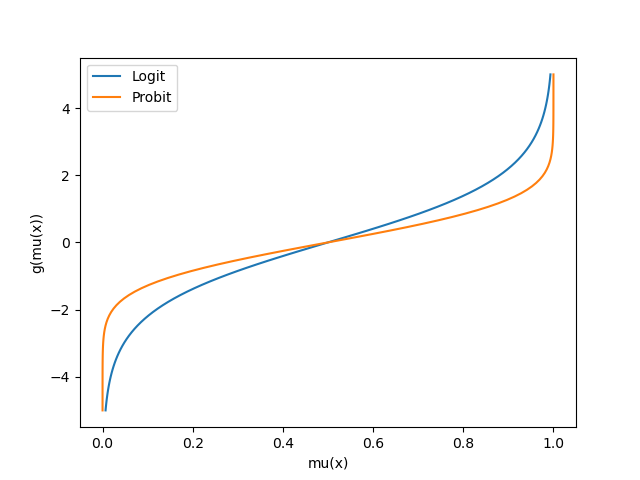
\includegraphics[scale=0.5]{img/probit_logit.png}
            \caption{Logit and Probit Functions}
            \label{fig:logit_probit}
        \end{figure}
    \end{enumerate}
    \end{example}

    Now there are many choices of functions we can take. In fact, if $\mu$ lives in $(0, 1)$, then we can really just take our favorite distribution that has a density that is supported everywhere in $\mathbb{R}$ and take the inverse cdf as our link. So far, we have no reason to prefer one function to another, but in the next section, we will see that there are more natural choices. 

    \subsubsection{Canonical Link Functions}

      Now let's summarize what we have. We assume that the conditional distribution $Y \mid X = x$ follows a distribution in the exponential family, which we can completely characterize by the cumulant generating function $\psi$. For different values of $x$, the conditional distribution will be paramaterized by different $\eta (x)$, and the resulting distribution $P_\eta$ will have some mean $\mu(x)$, which is usually not the natural parameter $\eta$. Now, let's forget about our knowledge that $\psi^\prime(\eta) = \mu$, but we know that there is some relationship between $\eta \leftrightarrow \mu$.

      Given an $x$, I need to use the linear predictor $x^T \beta$ to predict $\mu(x)$, which can be done through the link function $g$. 
      \[g\big( \mu(x) \big) = x^T \beta\]
      Now what would be a natural way of choosing this $g$? Note that our natural parameter $\eta$ for this canonical family takes value on the entire real line. I must construct a function $g$ that maps $\mu$ onto the entire real line, and so why not make it map to $\eta$. Therefore, we have 
      \[\eta(x) = g\big( \mu(x) \big) = x^T \beta\]

      \begin{definition}[Canonical Link]
      The function $g$ that links the mean $\mu$ to the canonical parameter $\theta$ is called the \textbf{canonical link}. 
      \[g(\mu) = \theta\]
      Now using our knowledge that $\psi^\prime(\eta) = \mu$, we can see that 
      \[g = (\psi^\prime)^{-1}\]
      This is indeed a valid link function. 
      \begin{enumerate}
          \item $\psi^{\prime\prime} > 0$ since it models the variance, and so $\psi^\prime$ is strictly increasing and so $g = (\psi^\prime)^{-1}$ is also strictly increasing. 
          \item The domain of $\psi^\prime$ is the real line since it takes in the natural parameter $\eta$ which exists over $\mathbb{R}$, so $\mathrm{Im}(g) = \mathbb{R}$. 
      \end{enumerate}
      \end{definition}

      So, given our cumulant generating function $\psi$ and our link function $g$, both satisfying 
      \[\psi^\prime (\eta) = \mu \text{ and } g(\mu) = x^T \beta\]
      we can combine them to get 
      \[(g \circ \psi^\prime) (\eta) = g(\mu) = x^T \beta\]
      and so, even though the mean of the response variable is not linear with respect to $x$, the value of $(g \circ \psi^\prime) (\eta)$ is indeed linear. In fact, if we choose the canonical link, then the equation 
      \[\eta = x^T \beta\]
      means that the natural parameter of our conditional distribution in the exponential family is linear with respect to $x$! From this we can find the conditional mean $\mu(x)$. 

      The reason we focus on canonical link functions is because, when the canonical link is used, the components of the model (the parameters of the linear predictor) have an additive effect on the response variable in the transformed (linked) scale, which makes the interpretation of the results easier. It's also worth noting that while using the canonical link function has some desirable properties, it is not always the best or only choice, and other link functions may be used if they provide a better fit for the data or make more sense in the context of the problem at hand.

      Let us evaluate some canonical link functions. 

      \begin{example}
      The Bernoulli has the canonical exponential form of 
      \[p_\eta (x) = \exp \big[ x \eta - \log (1 + e^\eta) \big]\]
      where $\eta = \log \big( \frac{\theta}{1 - \theta} \big)$. Since we have prior knowledge that $\theta = \mu$ (i.e. the expectation of a Bernoulli is the hyperparameter $\theta$ itself), we have a function that maps $\mu \mapsto \eta$. 
      \[\eta = g(\mu) = \log \bigg( \frac{\mu}{1 - \mu} \bigg)\]
      which gives us our result. We can also take the inverse of $\psi^\prime = \frac{e^\eta}{1 + e^\eta}$ to get our result 
      \[g (\mu) = (\psi^\prime)^{-1} (\mu) = \log \bigg( \frac{\mu}{1 - \mu} \bigg) \]
      \end{example}

  \subsection{Likelihood Optimization}

    Now let us have a bunch of data points $\{(x_n, y_n)\}_{n=1}^N$. By our model assumption, we know that the conditional distribution $Y \mid X = x_n$ is now of an exponential family with parameter $\eta_n = \eta (x_n)$ and density 
    \[p_{\eta_n} (y_n) = \exp \big[ y_n \eta_n - \psi(\eta_n) \big] h(y_n)\]
    Now we want to do likelihood optimization on $\beta$ (not $\eta$ or $\mu$), and to do this, we must rewrite the density function in a way so that it depends on $\beta$. Given a link function $g$, note the following relationship between $\beta$ and $\eta$: 
    \begin{align*}
        \eta_n = \eta (x_n) & = (\psi^\prime)^{-1} (\mu (x_n)) \\
        & = (\psi^{\prime})^{-1} \big( g^{-1} (x_n^T \beta )\big) \\
        & = h(x_n^T \beta) 
    \end{align*}
    where for shorthand notation, we define $h \coloneqq (g \circ \psi^\prime)^{-1}$. Subtituting this into the above likelihood, taking the product of all $N$ samples, and logarithming the equation gives us the following log likelihood to optimize over $\beta$. 
    \[\ell(\beta) = \log \prod_{n=1}^N p_{\eta_n} (y_n) = \sum_{n=1}^N y_n h(x_n^T \beta)  - \psi(h(x_n^T \beta) )\]
    where we dropped the $h(y_n)$ term at the end since it is a constant and does not matter. If $g$ was the canonical link, then $h$ is the identity, and we should have a linear relationship between $\eta (x_n) = x_n^T \beta$. This means that the $\eta_n$ reduces only to $x_n^T \beta$, which is much more simple to optimize. 
    \[\ell(\beta) = \log \prod_{n=1}^N p_{\eta_n} (y_n) = \sum_{n=1}^N y_n x_n^T \beta - \psi(x_n^T \beta)\]
    Note that the first term is linear w.r.t $\beta$, and $\psi$ is convex, so the entire sum must be concave w.r.t. $\beta$. With this, we can bring in some tools of convex optimization to solve. 

\section{Ensemble Methods}

    The bias variance noise decomposition gives us a very nice way of explaining overfittting. That is, the bias (expectation of the squared difference between the true $\mathbb{E}[Y \mid X]$ and the expected trained hypothesis function $h_{\boldsymbol{\theta}; \mathcal{D}}$) reduces, but the variance in this overfitted model increases. Therefore, if we had a slightly different dataset $\mathcal{D}$ sampled from $(X \times Y)^N$, then we might have a very different trained hypothesis since it's so sensitive to the data. 

    A way to treat this is through \textbf{ensemble learning}, where we train \textit{multiple} models over slightly different datasets, and then average their predictions to get a better model. What do we mean by a better model? Well, we know that a too complex model has low bias but large variance, and a too simple model has high bias but low variance. 

    \begin{enumerate}
      \item \textit{Bagging} refers to taking a complex model and decreasing its variance. Even though each model is trained over a smaller dataset, resulting it being more noisy, the average of all these slightly more noisy models will hopefully bring down the variance more than what we have added.\footnote{This is why random forests have underlying trees that are somewhat as large as possible.} 
      \item \textit{Boosting} refers to taking a simple model and decreasing its bias. Each simple model, usually a weak learner, has relatively small search space, but by taking the aggregate of them, we can hopefully increase it whilst bounding the variance in some way. Usually, the dataset is reweighted such that the weak learner in the next iteration will correct the previous weak learner. 
    \end{enumerate}

  \subsection{Bagging}

    Let's start off with the simpler of the two. 

    \begin{definition}[Bootstrap Aggregating]
      Given a dataset $\mathcal{D}$ of $N$ samples and a model $\mathcal{M}$, \textbf{bagging} is an ensemble method done with two steps: 
      \begin{enumerate}
        \item \textit{Bootstrap}. Sample $\Tilde{N}$ data points with replacement from $\mathcal{D}$ to get a dataset $\mathcal{D}_1$, and do this $M$ times to get 
        \[\mathcal{D}_1, \mathcal{D}_2, \ldots, \mathcal{D}_M \subset \mathcal{D}\]
        \item \textit{Aggregate}. For each sub dataset $\mathcal{D}_m$, train our model to get the optimal hypothesis $h_{\mathcal{D}_m}^\ast$. We should have $M$ different hypothesis functions, each trained on each sub dataset. 
        \[h_{\mathcal{D}_1}^\ast, h_{\mathcal{D}_2}^\ast, \ldots, h_{\mathcal{D}_M}^\ast\]
      \end{enumerate}
      To predict the output on a new value $\hat{\mathbf{x}}$, we can evaluate all the $h_{\mathcal{D}_m}^\ast (\hat{\mathbf{x}})$ .
    \end{definition}

    Note that the bootstrapping step could be expanded to different types of subsampling. 

    \begin{definition}[Pasting]
      If random subsets (without replacement) are sampled from the original dataset $\mathcal{D}$, then this method is known as \textbf{pasting}. 
    \end{definition}

    \begin{definition}[Random Subspaces]
      When random subsets of the data are drawn as random subsets of the features, then this is known as \textbf{random subspaces}. 
    \end{definition}

    \begin{definition}[Random Patches]
      When random subsets of both the data and the features are chosen, then this is known as \textbf{random patches}. 
    \end{definition}

    Since the whole point of this algorithm is to reduce variance, bagging does not really overfit. 

    \subsection{Random Forests}

      \begin{definition}[Random Forests]
        A \textbf{random forest} is a (random patch) bagging algorithm where the component models are decision trees.  
      \end{definition}

  \subsection{Boosting} 

        Now we delve more into the applied and computational aspects of machine learning. It's had a lot of empirical success and is more interesting from a theoretical perspective. It starts off with the \textit{weak learning assumption}, which we introduce in the context of classification with the misclassification loss function. It is actually a specific case of PAC learners. 

        \begin{definition}[Probability Approximately Correct Learner]
          A \textbf{PAC learning} is an algorithm that learns a function class $\mathcal{H}$ with parameter $\delta > 0$ if there exists an $\epsilon > 0$ and the algorithm can find a $f \in \mathcal{H}$ with probability at least $1 - \delta$ s.t.
          \begin{equation}
            R(f) \leq \epsilon 
          \end{equation}
          i.e. 
          \begin{equation}
            \mathbb{P}[ R(f) \leq \epsilon] \geq 1 - \delta
          \end{equation}
        \end{definition}

        This is quite a strong requirement, since it says that with probability at least $1 - \delta$ you must find an model $f$ that is correct with a probability of $1 - \epsilon$, i.e. $\epsilon$-good.

        \begin{definition}[Weak Learner]
          A \textbf{weak learner} is an algorithm that learns a function class $\mathcal{H}$ with parameter $\delta > 0$ if there exists an $\gamma > 0$ and the algorithm can find a $f \in \mathcal{H}$ s.t. 
          \begin{equation}
            \mathbb{P}[ R(f) < 1/2 - \gamma] \geq 1 - \delta
          \end{equation}
          for some $\delta > 0$, where $\gamma$ is considered our edge. Another way to write it is that with probability of at least $1 - \delta$, we can find a function $f$ s.t. 
          \begin{equation}
            \mathbb{P}_{x, y \sim \mathcal{X} \times \mathcal{Y}} [f(x) \neq y] < 1/2 - \gamma 
          \end{equation}
          This essentially means that given some $\gamma$ that measures how good our target predictor is compared to random guessing, the probability that we can find such a predictor with this edge is $1 - \delta$. Furthermore, this case must hold true for all distributions $P \sim \mathcal{X} \times \mathcal{Y}$. 
        \end{definition}

        Therefore, a weak learner just means some algorithm that learns a model that is a bit better than random. For example, learning decision stumps may be a weak learner. Colloquially, a weak learner can be thought of as an algorithm that cannot get your training error to $0$ and a strong learner can. The question is then, can we make a strong learner out of a bunch of weak learners? The general idea is that we want to iteratively find a bunch of weak learners and slowly add them up to get a strong learner. 
        \begin{equation}
          f = \sum_{i=1}^n f_i
        \end{equation}
        where $f$ is strong, $f_i$ weak. 

      \subsubsection{Adaptive Boosting (AdaBoost)} 

        Let's start with Adaboost for binary classification. 

        \begin{definition}[Adaboost for Binary Classification]
          Given data $\{(x_i, y_i)\} \in \mathcal{X} \times \mathcal{Y}$, with $\mathcal{Y} = \{-1, +1\}$, we implement the following greedy algorithm. 
          \begin{enumerate}
            \item You first set an $n$-vector weighting your samples, where the weight of the $i$th sample is $W_t (i)$. 
              \begin{equation}
                W_1 = \big( \frac{1}{n}, \ldots, \frac{1}{n} \big)
              \end{equation}

            \item For $t = 1, \ldots, T$, we do the following. 
              \begin{enumerate}
                \item You run your weak learning algorithm, which will return your hypothesis $h_t$ with probability $1 - \delta$ which is slightly better than random. We define its empirical error over the distribution $W_t$ to be 
                  \begin{equation}
                    \epsilon_t = R_{W_t} (h_t) = \mathbb{P}_{x_i \sim W_t} [ h_t (x_i) \neq y_i] = \sum_{i=1}^n W_t (i) \cdot \mathbbm{1}_{h_t (x_i) \neq y_i}
                  \end{equation}
                  This may be done differently by actually sampling $n$ samples from this distribution and then computing proportion of misclassifications. 

                \item This new weak learner provides some information on the new weighted distribution. We would like to weight this weak learner $h_t$ with some scale $\alpha_t$ to determine how important its vote is in the ensemble. We define this weighting to be 
                  \begin{equation}
                    \alpha_t = \frac{1}{2} \ln \bigg( \frac{1 - \epsilon_t}{\epsilon_t} \bigg)
                  \end{equation}
                Note the following important properties. If $0 < \epsilon_t < 0.5$, then this does indeed mean that $h_t$ is slightly better than random, so it would have a positive weighting. If $\epsilon_t = 0.5$, then it is random so no weighting. Finally, if $0.5 < \epsilon < 1.0$, then it is an extremely poor classifier and we are better off looking at the opposite of its prediction, meaning that $\alpha_t$ will be negative.
                This is also seen with the facts that as $\epsilon_t \rightarrow 0, 1$, then $\alpha_t \rightarrow +\infty, -\infty$.\footnote{In practice, $\epsilon$ cannot be $0$ or $1$ due to numerical reasons, so a small constant is added to prevent this from happening.} 

                \item Then we set 
                  \begin{equation}
                    W_{t + 1} (i) \propto W_t (i) \, \exp\{ - \alpha_t y_i h_t (x_i) \} = \begin{cases} 
                      e^{-\alpha_t} & \text{ if } h_t(x_i) = y_i\\  
                      e^{+\alpha_t} & \text{ if } h_t (x_i) \neq y_i
                    \end{cases}
                  \end{equation}
                  meaning that the new weights go up for incorrect labels and down for correct labels. We show proportional to since it is not normalized, but we can normalize it with the constant $Z_t$. 
              \end{enumerate}

            \item Your final strong classifier is then 
              \begin{equation}
                f(x) = \mathrm{sign} \bigg( \sum_{t=1}^T \alpha_t h_t(x) \bigg)
              \end{equation}
              which indeed is a sequential sum of these classifiers. 
          \end{enumerate}
        \end{definition}

        In this way, by weighting the incorrect labels higher, I am telling successive weak learner to give me a new weak hypothesis that tells me something new. This makes it so that the actual sequence of learned weak models are important, since the next $h_{t+1}$ tries to fix the errors that the $h_t$ makes. 

        \begin{algo}[AdaBoost Algorithm]
          The full algorithm for brevity is shown below. 
          \begin{algorithm}[H]
            \label{alg:adaboost}
            \begin{algorithmic}[1]
              \Require Training data $\{(x_i, y_i)\}_{i=1}^n$ where $x_i \in \mathcal{X}$, $y_i \in \{-1, +1\}$
              \Require Number of iterations $T$
              \Require Weak learning algorithm $\mathcal{A}$

              \State Initialize weights $W_1(i) = \frac{1}{n}$ for $i = 1,\ldots,n$

              \For{$t = 1$ to $T$}
                \State Train weak learner $h_t = \mathcal{A}(\{(x_i, y_i)\}, W_t)$
                
                \State Calculate weighted error:
                \State $\epsilon_t = \sum_{i=1}^n W_t(i) \cdot \mathbbm{1}_{h_t(x_i) \neq y_i}$
                
                \If{$\epsilon_t \geq \frac{1}{2}$}
                    \State break
                \EndIf
                
                \State Calculate importance weight:
                \State $\alpha_t = \frac{1}{2} \ln(\frac{1-\epsilon_t}{\epsilon_t})$
                
                \State Update sample weights:
                \For{$i = 1$ to $n$}
                    \State $W_{t+1}(i) = W_t(i) \cdot \exp(-\alpha_t y_i h_t(x_i))$
                \EndFor
                
                \State Normalize weights:
                \State $Z_t = \sum_{i=1}^n W_{t+1}(i)$
                \State $W_{t+1}(i) = \frac{W_{t+1}(i)}{Z_t}$ for all $i$
              \EndFor

              \State \Return Final classifier $f(x) = \text{sign}\left(\sum_{t=1}^T \alpha_t h_t(x)\right)$
            \end{algorithmic}
          \end{algorithm}
        \end{algo}

        We now actually show that this is a strong learner by showing that the training error goes to $0$. 

        \begin{theorem}[Exponential Decay of Training Error in AdaBoost]
          Support that $\gamma \leq (1/2) - \epsilon_t$ for all $t$. Then our empirical risk decays exponentially with $T$. 
          \begin{equation}
            \hat{R} (h) \leq e^{-2 \gamma^2 T}
          \end{equation}
          and hence, the training error goes to $0$ quickly. 
        \end{theorem}
        \begin{proof}
          Can be shown with the lemma. 
          \begin{equation}
            Z_t = 2 \sqrt{\epsilon_t (1 - \epsilon_t)}
          \end{equation}
        \end{proof}

        Sure, the training error goes to $0$, but what we really care about is the generalization error. It turns out that we can prove things about this, but omitted for now. 

        \begin{example}[AdaBoost with Stumps]
          We can define our weak learning algorithm to be a decision stump with only 1 split. Doing adaboost gives something similar to a random forest (but not quite since its a bagging algorithm) with great generalization error. 
        \end{example}

        Surprisingly, Adaboost has a tendency not to overfit, i.e. the variance does not explode. There is a lot of theory that tries to explain why this is the case, such as margin theory. 

        There are a lot of different ways to analyze AdaBoost. For many years, researchers did not think of it as having any connection to gradient descent or loss functions, but it actually does. AdaBoost can be viewed as optimizing the \textbf{exponential loss} 
        \begin{equation}
          L(\mathbf{x}, y) = e^{-y f(\mathbf{x})} 
        \end{equation}
        so that the full empirical objective function is 
        \begin{equation}
          L = \sum_i \exp \bigg( -\frac{1}{2} y_i \, \sum_{t=1}^T \alpha_t f_t (\mathbf{x}_i)\bigg)
        \end{equation}
        which must be optimize w.r.t. the weights $\alpha_t$ and the parameters of each weak classifier $f_t$. This stepwise optimization is greedy and sequential, where we add one weak classifier at a time, choosing its parameters and $\alpha_t$ to be optimal w.r.t. $L$ and then never change it again. It turns out that if we actually do keep things constant and solve the optimal parameters, it must be the case that $\alpha_t = \ln \frac{1 - \epsilon_t}{\epsilon_t}$, which is why it is in the algorithm.\footnote{Derivation \href{https://www.cs.toronto.edu/~mbrubake/teaching/C11/Handouts/AdaBoost.pdf}{here}} Furthermore, the exponential loss is an upper-bound on the misclassification loss, so if an exponential loss of $0$ is achieved, then all training points are correctly classified. 

      \subsubsection{Gradient Boosting}

        Gradient boosting can deal with both regression and classification problems, and so we will present it in full generality. 

        \begin{definition}[Gradient Boosting]
          Let us have data $\{(x_i, y_i)\} \in \mathcal{X} \times \mathcal{Y}$ and a differentiable loss function 
          \begin{equation}
            L(\mathbf{y}, \hat{\mathbf{y}}) = \sum_{i=1}^n L(y_i, \hat{y}_i)
          \end{equation}
          with also a \textit{constant} stepsize $\eta$. 

          \begin{enumerate}
            \item We first initialize the model with a constant value that minimizes the loss. So we have a single leaf as in our decision tree ensemble. 
              \begin{equation}
                F_0 = \argmin_\gamma \sum_{i=1}^n L(y_i, \gamma)
              \end{equation}
              If we're doing regression with the MSE loss, then $\gamma = \bar{y}$, the average. This is our first predictor, which predicts $F_0 (x) = \gamma$ for all $x$, and so $F_0$ is really just the constant $n$-vector $(\bar{y}, \ldots, \bar{y})$. If we're doing binary classification, we can focus on the logits and initialize $\gamma$ as the log-odds $\log(\frac{C_+}{C_{-}})$

            \item For $t = 1, \ldots, T$, we do the following. 
              \begin{enumerate}
                \item We have the predicted values $F_{t-1}(x_i)$ for each sample $x_i$. We compute the negative gradient of the loss function w.r.t. the predicted value.
                  \begin{equation}
                    \mathbf{r}_t = - \frac{\partial L(\mathbf{y}, \hat{\mathbf{y}})}{\partial \hat{\mathbf{y}}} \bigg|_{\hat{y} = F_{t-1} (\mathbf{x})} = - \bigg( \frac{\partial L(y_1, \hat{y}_1)}{\partial \hat{y}_1} \bigg|_{\hat{y}_1 = F_{t-1} (x_1)}, \ldots, \frac{\partial L(y_n, \hat{y}_n)}{\partial y_n} \bigg|_{\hat{y}_n = F_{t-1}(x_n)} \bigg)
                  \end{equation}
                  Note that the vector above is a $n$-vector, and when we use the MSE loss, then the gradient just simplifies to the residual.  

                \item We use our weak learning algorithm to train a weak model $f_t$ on the residual values $\mathbf{r}_t$. 

                \item We update  
                  \begin{equation}
                    F_t = F_{t-1} + \eta \cdot f_t
                  \end{equation}
              \end{enumerate}
            \item In the end, we have 
              \begin{equation}
                F_t = F_0 + \eta f_1 + \eta f_2 + \ldots + \eta f_T
              \end{equation}
              consisting of a bunch of weak learners to make a strong learner. 
          \end{enumerate}
        \end{definition}

        In a way, we can think of this as an optimization problem in $\mathbb{R}^n$ (not $\mathbb{R}^d$!). We can think of $\hat{\mathbf{y}}$ representing the actual function $f$, and we're really doing gradient descent on the ``function space'' $\mathbb{R}^n$ by updating $F_t$. 

        \begin{algo}[Gradient Boosting]
          Here is the full algorithm for brevity. 
          \begin{algorithm}[H]
            \label{alg:gradboost}
            \begin{algorithmic}[1]
              \Require Training data $\{(x_i, y_i)\}_{i=1}^n$ where $x_i \in \mathcal{X}$, $y_i \in \mathcal{Y}$
              \Require Differentiable loss function $L(y, \hat{y})$
              \Require Number of iterations $T$
              \Require Learning rate $\eta$
              \Require Weak learning algorithm $\mathcal{A}$

              \State // Initialize model with optimal constant value
              \State $F_0 = \argmin_\gamma \sum_{i=1}^n L(y_i, \gamma)$
              \State // For regression (MSE): $F_0 = \frac{1}{n}\sum_{i=1}^n y_i$
              \State // For binary classification: $F_0 = \log(\frac{C_+}{C_-})$

              \For{$t = 1$ to $T$}
                  \State // Compute negative gradient vector
                  \For{$i = 1$ to $n$}
                      \State $r_{t,i} = -\frac{\partial L(y_i, \hat{y}_i)}{\partial \hat{y}_i}\big|_{\hat{y}_i = F_{t-1}(x_i)}$
                  \EndFor
                  
                  \State // Train weak learner on pseudo-residuals
                  \State $f_t = \mathcal{A}(\{(x_i, r_{t,i})\}_{i=1}^n)$
                  
                  \State // Update model with scaled weak learner
                  \For{$i = 1$ to $n$}
                      \State $F_t(x_i) = F_{t-1}(x_i) + \eta \cdot f_t(x_i)$
                  \EndFor
              \EndFor

              \State \Return Final model $F_T(x) = F_0(x) + \eta \sum_{t=1}^T f_t(x)$

              \State // Special cases for common loss functions:
              \State // For MSE: $r_{t,i} = y_i - F_{t-1}(x_i)$ (actual residual)
              \State // For LogLoss: $r_{t,i} = y_i - \sigma(F_{t-1}(x_i))$ where $\sigma$ is sigmoid
            \end{algorithmic}
          \end{algorithm}
        \end{algo}

        \begin{example}[Regression Trees]
          If we have regression trees as our weak learners (pratically the max depth is 8 to 32 rather than stumps) with the L2 loss function.  
          \begin{enumerate}
            \item The initial model will just constantly predict the average of the $y_i$'s. 
            \item The $r_t$ are just the pseudoresiduals
              \begin{equation}
                r_t = -\big( y_1 - f_{t-1} (x_1), \ldots, y_n - f_{t-1} (x_n) \big)
              \end{equation}
            \item In case where there are multiple samples running to the same leaf node, the predicted values of the terminal nodes are the average of the $y$'s of those samples. 
          \end{enumerate}
        \end{example}

        \begin{example}[Gradient Boosting Classification] 
          If we have classification trees as our weak learners, then 
          \begin{enumerate}
            \item The initial model will just constantly predict the log odds $\log(C_{+} / C_{-})$, where $C_{\pm}$ is the number of ones and zeros in the whole dataset. For multiclass there is probably a softmax variant of this. 
            \item In case where there are multiple samples running to the same leaf node, the predicted values of the terminal nodes are decided by majority. 
          \end{enumerate}
        \end{example}

        The general ideas are pretty much the same between AdaBoost and gradient boost. We iteratively build a strong learner from weak learners. A few differences, however, 
        \begin{enumerate}
          \item AdaBoost dynamically weighs the importance of each weak model, while gradient boost weak learners are equally weighted by $\eta$. 
          \item AdaBoost actively focuses on the samples where the previous weak learner got wrong, but gradient boost reduces the whole loss in general. 
          \item Gradient boost usually uses trees larger than stumps. 
        \end{enumerate}

      \subsubsection{XGBoost} 

        The final mainstream boosting algorithm is XGBoost. In regression, XGBoost fits to the residuals just like gradient boosting, but it uses unique regression trees. It is designed for large, complex datasets. 

        \begin{definition}[XGBoost for Regression] 
          Let us have the same data $\{(x_i, y_i)\} \in \mathcal{X} \times \mathcal{Y}$ and the MSE loss 
          \begin{equation}
            L(\mathbf{y}, \hat{\mathbf{y}}) = \frac{1}{2} \sum_{i=1}^n (y_i - \hat{y}_i)^2
          \end{equation}
          with a constant stepsize $\varepsilon$ (by default $3$). 

          \begin{enumerate}
            \item We first initialize the model with a constant value that minimizes the loss, which is just the average. So we have a single leaf as in our decision tree ensemble. 
              \begin{equation}
                F_0 = \bar{y}
              \end{equation}

            \item For $t = 1, \ldots, T$, we do the following. 
              \begin{enumerate}
                \item We have the predicted values $F_{t-1}(x_i)$ for each sample. We first compute the residuals, denoted $\mathbf{r}_0$. To build our next tree, we start off with a single node ``containing'' this set of residuals representing each data point. 

                \item We want to grow the decision tree, and we do this by splitting on the maximum gain in \textit{similarity score}, defined for a collection of residuals $\mathbf{r}$ to be 
                \begin{equation}
                  s(\mathbf{r}) = \frac{\sum r_i}{\mathrm{dim}(\mathbf{r}) + \lambda}
                \end{equation}
                This score determines how well the set is clustered, and we would like well clustered residuals to be close together.$\lambda$ is a regularization parameter used to decrease the score's sensitivity when splitting. Therefore, we first compute the score for the root node, and let us define the score of a tree as the sum of the scores of all its leaves. We want to split greedily on this metric. We can keep on splitting until it reaches a certain number of levels (6), and then we can prune it based on whether the increase in score surpasses a threshold, called the \textit{gain}. Note that as $\lambda$ increases, it is easier to prune the tree. 

                \item With our trained tree $f_t$, we add it to our cluster to iteratively build our final predictor. 
                  \begin{equation}
                    F_t = F_{t-1} + \varepsilon \cdot f_t
                  \end{equation}

              \end{enumerate}
          \end{enumerate}
        \end{definition}


\section{Clustering and Density Estimation} 

  \subsection{K Means Clustering} 

    The simplest type of unsupervised learning is \textbf{clustering}. In the clustering problem, we are given a training set of \textit{unlabeled} data

    \begin{equation}
      \{ \mathbf{x}^{(1)}, \mathbf{x}^{(2)}, \ldots, \mathbf{x}^{(n)}\}
    \end{equation}
    and want to group the data into a few cohesive ``clusters.''

    \begin{enumerate}
      \item Determine the number of clusters that we want to find and set it as $k$ (this can be a disadvantage if we do not know how many clusters we are looking for beforehand).

      \item We initialize the \textbf{cluster centroids} $\boldsymbol{\mu}_1, \boldsymbol{\mu}_2, \ldots, \boldsymbol{\mu}_k \in \mathbb{R}^d$ randomly or by some other method.

      \item The next part takes the centroids and moves them to the center of each cluster accordingly. The following two steps are repeated until convergence (and convergence is guaranteed):
        \begin{enumerate}
          \item We assign each training sample $\mathbf{x}^{(i)}$ to the closest cluster centroid $\boldsymbol{\mu}_j$. That is, for every $i = 1, \ldots, n$, set
            \begin{equation}
              c^{(i)} \equiv \text{arg}\; \min_j || \mathbf{x}^{(i)} - \boldsymbol{\mu}_j ||^2
            \end{equation}
          where this $\text{argmin}$ function returns the input to a function that yields the minimum (in this case, the number $j$ that yields the minimum value of $|| \mathbf{x}^{(i)} - \boldsymbol{\mu}_j ||^2$ for each $i$).

          \item We move each training cluster centroid $\boldsymbol{\mu}_j$ to the mean of the points assigned to it. That is, for each $j = 1, \ldots, k$, set 
            \begin{equation}
              \boldsymbol{\mu}_j \equiv \frac{\sum_{i=1}^n 1\{c^{(i)} = j\}\, \mathbf{x}^{(i)}}{\sum_{i=1}^n 1 \{c^{(i)} = j\}}
            \end{equation}
        \end{enumerate}
    \end{enumerate}

    \begin{figure}[H]
      \centering 
      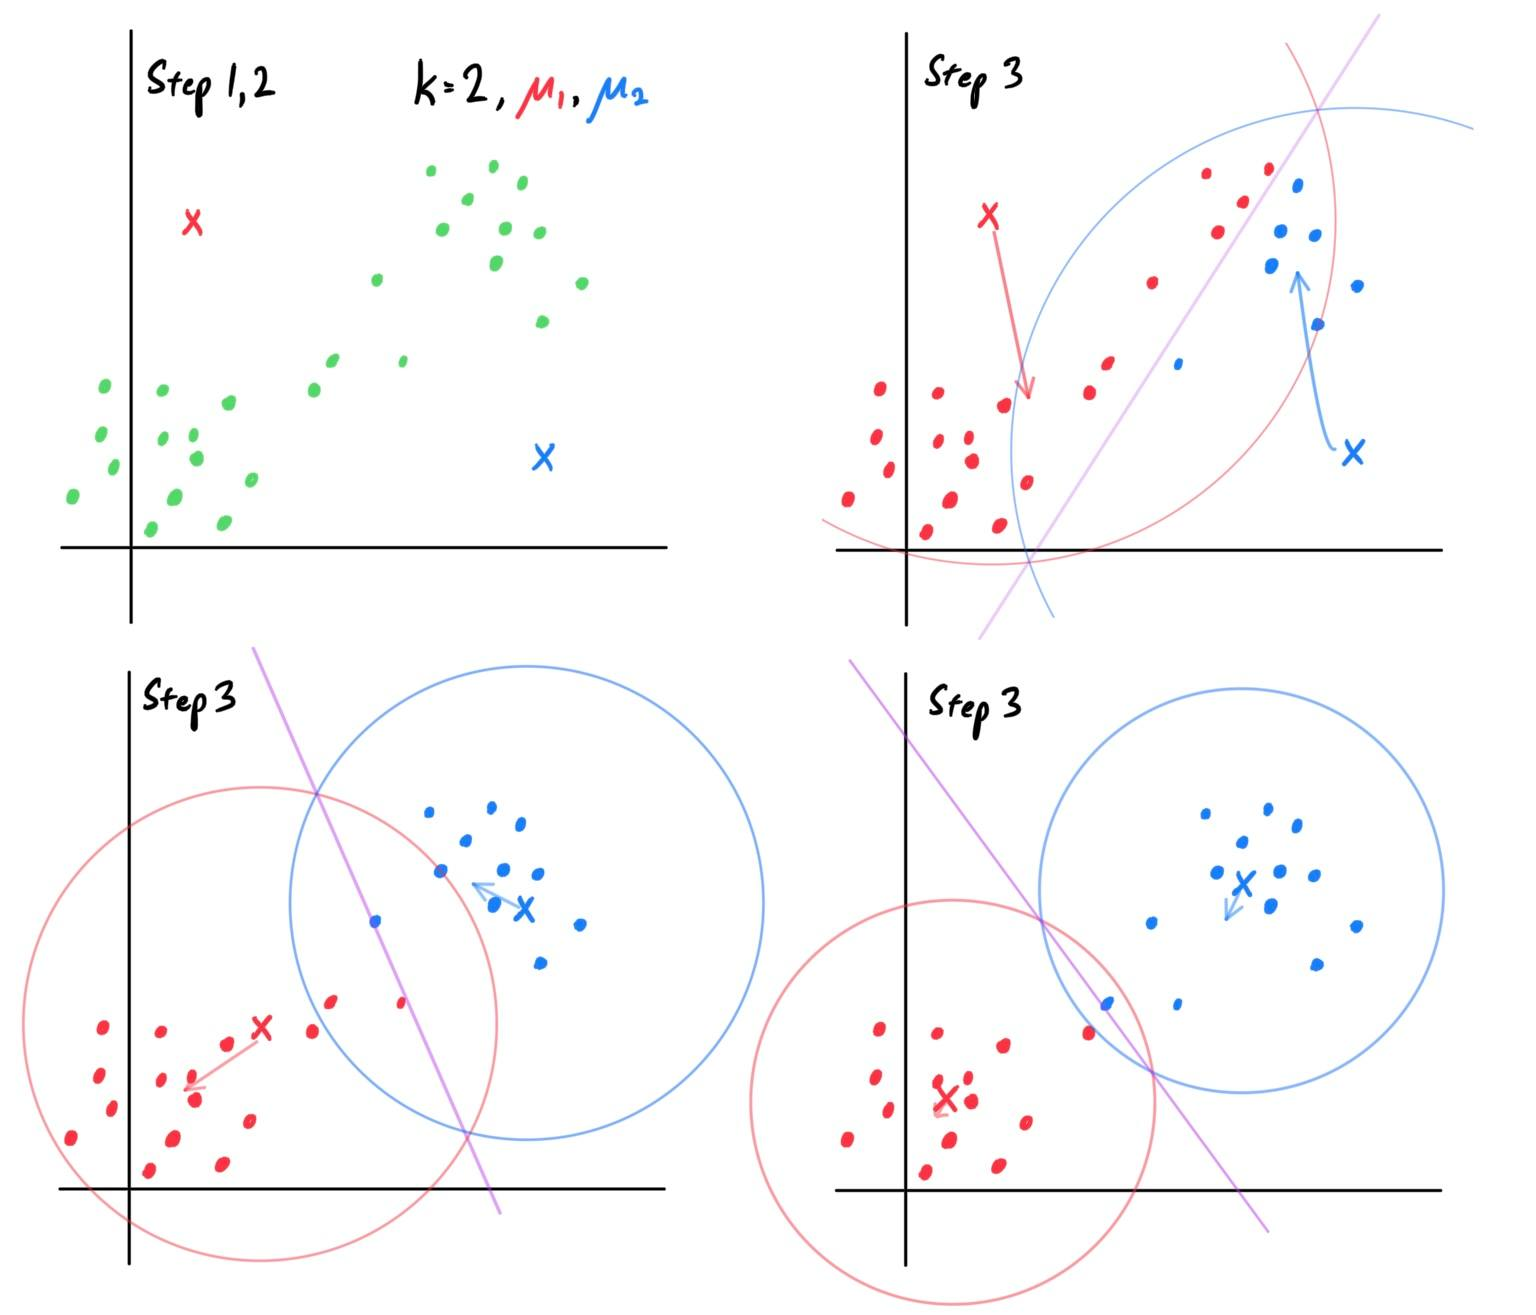
\includegraphics[scale=0.25]{img/k_means_clustering.jpg}
      \caption{The steps can be visualized for a set of unlabeled data (green points) in $\mathbb{R}^2$ clustered into $k=2$ groups (red and blue). The crosses represent the cluster centroids.} 
      \label{fig:k_means_clustering}
    \end{figure}

    We can interpret this algorithm in another equivalent way. $k$-means is precisely coordinate descent on the cost function called the \textbf{distortion function}: 
    \begin{equation}
      L(\boldsymbol{\mu}_1, \ldots, \boldsymbol{\mu}_k) \equiv \sum_{i=1}^n \min_k ||\mathbf{x}^{(i)} - \boldsymbol{\mu}_k ||^2
    \end{equation}
    but since $L$ is not necessarily convex, it might be susceptible to local extrema.

  \subsection{Gaussian Mixture Models and EM Algorithm}

      Given a training set ${\mathbf{x}^{(i)}}_{i=1}^n$ (without the $y$-labels and so in the unsupervised setting), there are some cases where it may seem like we can fit multiple Gaussian distributions in the input space $\mathcal{X}$. For example, the points below seem like they can be fitted well with 3 Gaussians.

      \begin{figure}[H]
        \centering
        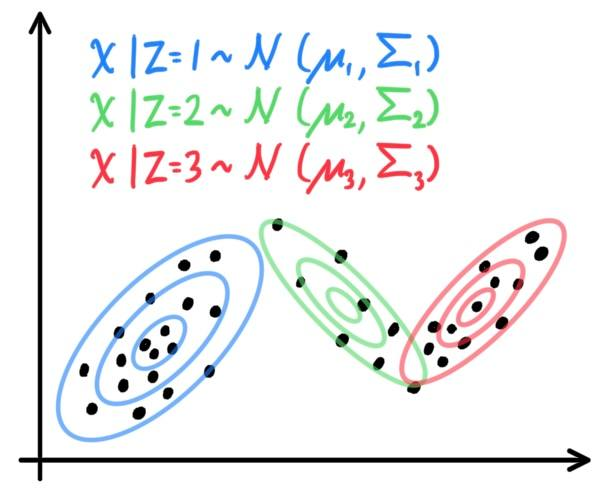
\includegraphics[width=0.4\textwidth]{img/mixture_of_gaussians_example.jpg}
        \caption{Example of data that can be fitted with 3 Gaussians}
      \end{figure}

      Therefore, we can construct a best-fit model as a composition of a multinomial distribution (to decide which one of the Gaussians $\mathbf{x}$ should follow) followed by a Gaussian. That is, to find the distribution of $\mathbf{x}$ and get the density function $p(\mathbf{x})$, we condition it on the random variable $Z$. More specifically, we let

      \[Z \sim \text{Multinomial}(\boldsymbol{\phi}), \;\;\;\;\; \boldsymbol{\phi} = \begin{pmatrix} \phi_1 \ \phi_2 \ \ldots \ \phi_k \end{pmatrix} \text{ such that } \sum_{i=1}^k \phi_i = 1\]
      and define the conditional distributions as
      \begin{align*}
        \mathbf{X} \mid Z = 1 & \sim \mathcal{N}(\boldsymbol{\mu}_1, \boldsymbol{\Sigma}_1) \\
        \mathbf{X} \mid Z = 2 & \sim \mathcal{N}(\boldsymbol{\mu}_2, \boldsymbol{\Sigma}_2) \\
        \ldots & \sim \ldots \\
        \mathbf{X} \mid Z = j & \sim \mathcal{N}(\boldsymbol{\mu}_j, \boldsymbol{\Sigma}_j) \\
        \ldots & \sim \ldots \\
        \mathbf{X} \mid Z = k & \sim \mathcal{N}(\boldsymbol{\mu}_k, \boldsymbol{\Sigma}_k)
      \end{align*}
      Therefore, our model says that each $\mathbf{x}^{(i)}$ was generated by randomly choosing $z^{(i)}$ from ${1, \ldots, k}$ according to some multinomial, and then the $\mathbf{x}^{(i)}$ was drawn from one of the $k$ Gaussians depending on $z^{(i)}$. This model is called the \textbf{mixture of Gaussians model}. The parameters of our model are: 

      \begin{itemize}
        \item The vector $\boldsymbol{\phi} \in \mathbb{R}^k$ (which really has $k-1$ parameters) characterizing the multinomial distribution.
        \item The set of vectors $\boldsymbol{\mu}_1, \boldsymbol{\mu}_2, \ldots, \boldsymbol{\mu}_k$ representing the mean vectors of each multivariate Gaussian. For simplicity, we'll denote this set of vectors as $\bm{\mu}$.
        \item The set of symmetric, positive-definite matrices $\boldsymbol{\Sigma}_1, \boldsymbol{\Sigma}_2, \ldots, \boldsymbol{\Sigma}_k$ representing the covariance matrices of each multivariate Gaussian. For simplicity, we'll denote this set of matrices as $\bm{\Sigma}$.
      \end{itemize}

      We can write down the log-likelihood of the given data $\mathbf{x}^{(i)}$'s as a function of all the parameters above as:

      \begin{align*}
        l (\boldsymbol{\phi}, \bm{\mu}, \bm{\Sigma}) & = \sum_{i=1}^n \log, p\big( \mathbf{x}^{(i)} ;  \boldsymbol{\phi}, \bm{\mu}, \bm{\Sigma} \big) \\
        & = \sum_{i=1}^n \log \bigg( \sum_{j=1}^k  p\big( \mathbf{x}^{(i)} \mid z^{(i)} = j ; \bm{\mu}, \bm{\Sigma} \big) , p\big( z^{(i)} = j; \boldsymbol{\phi}\big) \bigg)
      \end{align*}

      This equation above tells us the (log-) likelihood of the data landing on the $\mathbf{x}^{(i)}$'s given that we have parameters $\boldsymbol{\phi}, \bm{\mu}, \bm{\Sigma}$. Note that since we only know that the \textit{final} value of the $i$th sample is $\mathbf{x}^{(i)}$ and not anything at all about which value $z^{(i)}$ the $i$th sample had, there is an extra unknown in this model. That is, we do not know which one of the $k$ Gaussians the $\mathbf{x}^{(i)}$ was generated from. These values $z^{(i)}$ are called the \textbf{hidden/latent variables}.

      If we did know the values of the hidden variables $z^{(i)}$ (i.e. if we knew which of the $k$ Gaussians each $\mathbf{x}^{(i)}$ was generated from), then our log likelihood function would be much more simple since now, our givens will be both $\mathbf{x}^{(i)}$ \textit{and} $z^{(i)}$. Therefore, we don't have to condition on the $z^{(i)}$ and can directly calculate the log of the probability of us having sample values $(z^{(1)}, \mathbf{x}^{(1)}), (z^{(2)}, \mathbf{x}^{(2)}), \ldots, (z^{(n)}, \mathbf{x}^{(n)})$.

      \begin{align*}
        l(\boldsymbol{\phi}, \bm{\mu}, \bm{\Sigma}) & = \sum_{i=1}^n \log , p\big( \mathbf{x}^{(i)}; \boldsymbol{\phi}, \bm{\mu} ,\bm{\Sigma}\big) \\
        & = \sum_{i=1}^n \log, p\big( \mathbf{x}^{(i)}, z^{(i)}; \boldsymbol{\phi}, \bm{\mu} ,\bm{\Sigma}\big) \\
        & = \sum_{i=1}^n \log, p\big( \mathbf{x}^{(i)} \mid z^{(i)}; \bm{\mu}, \bm{\Sigma}) \; p\big( z^{(i)}; \boldsymbol{\phi} \big)
      \end{align*}

      This model, with known $z^{(i)}$'s, is basically the GDA model, which is easy to calculate. That is, the maximum values of $\boldsymbol{\phi}, \bm{\mu}, \bm{\Sigma}$ are:

      \begin{align*}
        \phi_j & = \frac{1}{n} \sum_{i=1}^n \mathbbm{1}_{z^{(i)} = j} \\
        \boldsymbol{\mu}_j & = \frac{\sum_{i=1}^n \mathbbm{1}_{z^{(i)} = j} \mathbf{x}^{(i)}}{\sum_{i=1}^n \mathbbm{1}_{z^{(i)} = j}} \\
        \boldsymbol{\Sigma}_j & = \frac{1}{\sum_{i=1}^n \mathbbm{1}_{z^{(i)} = j}} \sum_{i=1}^n \mathbbm{1}_{z^{(i)}} \big( \mathbf{x}^{(i)} - \boldsymbol{\mu}_j \big),\big(\mathbf{x}^{(i)} - \boldsymbol{\mu}_j \big)^T
      \end{align*}

      for $j = 1, \ldots, d$. But since we do \textit{not} know the values of $z^{(i)}$, we first try to "guess" the values of the $z^{(i)}$'s and then update the parameters of our model assuming our guesses are correct. Let us clarify some notation:

      \begin{itemize}
        \item The distribution that we will iteratively reassign over and over again is $Z$, with density $p_Z (z)$ that maps $z \mapsto \phi_z$, where $\boldsymbol{\phi}$ is a vector that represents the density. The algorithm will initialize $p_Z$ and have it converge to the true multinomial density. Note that $Z$ in this context could represent the true multinomial distribution $Z$ or could represent the distributions iteratively produced by the algorithm that should converge onto the true $Z$ (usually the latter).

        \item The $k$ Gaussian distributions that we will iteratively reassign over and over again is $\mathcal{N}_1, \mathcal{N}_2, \ldots, \mathcal{N}k$, with densities $p_{\mathcal{N}1}(\mathbf{x}), \ldots, p_{\mathcal{N}k}(\mathbf{x})$ that maps $\mathbf{x} \mapsto p_{\mathcal{N}j}(\mathbf{x})$.

        \item The distribution of the entire random variable $\mathbf{X}$ will have density $p_X(\mathbf{x})$. Since we are iteratively reassigning the densities $p_Z$ and $p{\mathcal{N}_j}$, this joint distribution of $\mathbf{X}$ will also get modified.
      \end{itemize}

      \begin{definition}[EM Algorithm]
        The \textbf{Expectation-Maximization (EM) Algorithm} has the following steps:

        \begin{enumerate}
          \item We initialize our values of $\theta$, which can be chosen randomly or by \textbf{K-means initialization} (not explained here).
          \begin{itemize}
            \item We can randomly assign our values of $\mu_j$'s and the $\Sigma_j$'s in $\mathbb{R}^d$.
            \item We can randomly assign the density of our guess multinomial $p_Z(z)$, represented by vector
            \[\phi = \begin{pmatrix} \phi_1 \\ \vdots \\ \phi_k \end{pmatrix} \text{ with } \sum_{j=1}^k \phi_j = 1\]
            where $p_Z(z) \equiv \phi_z$ for $z = 1, \ldots, k$.
          \end{itemize}

          \item \textbf{(E Step)} Now that we have our prior guess of what $Z$ and its density function $p_Z$ is, we can calculate its posterior density function by taking one observed example $x^{(i)}$ and modifying $p_Z$ to $p_Z^{(i)}$. This superscript $(i)$ on the distribution $p_Z$ indicates that this is a posterior density created from observing $x^{(i)}$. (The motivation for this construction is explained more specifically in the next section involving Jensen's inequality.) Using Bayes' rule, we should calculate $n$ density functions
          \[p_Z^{(i)}(z) \equiv p_Z(z\,|\,x^{(i)}; \phi, \mathbf{\mu}, \mathbf{\Sigma}) \text{ for } i = 1, \ldots, n\]
          For easier notation, we let $\phi^{(i)}$ be the vector representation of the density $p_Z^{(i)}$. That is,
          \[\phi^{(i)} = \begin{pmatrix} \phi_1^{(i)} \\ \vdots \\ \phi_k^{(i)} \end{pmatrix} \text{ with } \sum_{j=1}^k \phi_j^{(i)} = 1\]
          where $p_Z^{(i)}(z) \equiv \phi^{(i)}_z$ for $z = 1, \ldots, k$ and $0$ otherwise. Then, we can calculate $\phi^{(i)}$ (and therefore $p_Z^{(i)}$) component-wise by calculating each $\phi_j^{(i)}$ (which is the probability of a point being in the $j$th cluster, given that we observe example $x^{(i)}$):
          \begin{align*}
              \phi_j^{(i)} &= p_Z^{(i)}\big(z = j;\, \phi, \mathbf{\mu}, \mathbf{\Sigma}\big) \\
              &= p_Z\big(z = j\,|\,x^{(i)};\,\phi, \mathbf{\mu}, \mathbf{\Sigma}\big) \\
              &= \frac{p_{\mathcal{N}_j}\big(x^{(i)}\,|\,z^{(i)} = j;\,\mathbf{\mu}, \mathbf{\Sigma}\big) \; p_Z\big(z^{(i)} = j;\,\phi\big)}{p_X\big(x^{(i)};\,\phi, \mathbf{\mu}, \mathbf{\Sigma}\big)} \\
              &= \frac{p_{\mathcal{N}_j}\big(x^{(i)}\,|\,z^{(i)} = j;\,\mathbf{\mu}, \mathbf{\Sigma}\big) \; p_Z\big(z^{(i)} = j;\,\phi\big)}{\sum_{l=1}^k p_{\mathcal{N}_j}\big(x^{(i)}\,|\,z^{(i)} = l;\,\mathbf{\mu}, \mathbf{\Sigma}\big)\; p_Z\big(z^{(i)} = l;\,\phi\big)}
          \end{align*}
          Note that we have everything we need to calculate the posterior probability distribution $p_Z^{(i)}(z)$ of a point being in any cluster.
          \begin{itemize}
              \item $p_{\mathcal{N}_j}(x^{(i)}\,|\,z^{(i)} = j)$ represents the conditional Gaussian density, which is completely defined because the parameters $\mu_j, \Sigma_j$ are already defined in initialization.
              \item $p_Z(z^{(i)} = j; \phi)$ is really just the probability $\phi_j$ that a given point is in the $j$th cluster, which we've also defined in initialization.
              \item $p_X(x^{(i)})$ represents the distribution of the entire random variable $X$ of the entire training set. Knowing the first two and taking the sum gives this density function $p_X$.
          \end{itemize}
          Therefore, we should end up with $n$ different $k$-vectors $\phi^{(1)}, \phi^{(2)}, \ldots, \phi^{(n)}$, each representing our best guess of what multinomial density $p_Z^{(i)}$ each $x^{(i)}$ had followed in order to be at the given points.

          Let us elaborate further on the intuition of this step. In the normal GDA with given values of $z^{(i)}$, we have
          \[\phi_j = \frac{1}{n} \sum_{i=1}^n 1\{z^{(i)} = j\} = \frac{1}{n}\big(\text{Number of Samples in }j\text{th Gaussian}\big)\]
          which is a sum of "hard" guesses, meaning that each $x^{(i)}$ is undoubtedly in cluster $j$ or not, and so to find out our best guess for the true vector $\phi$, all we have to do is find out the proportion of all examples in each of the $k$ groups and we're done (without needing to iterate). However, in our EM model, we do not know the $z^{(i)}$'s, and so the best we can do is give the \textit{probability} $\phi^{(i)}_j$ that $x^{(i)}$ is in cluster $j$.

          \begin{figure}[H]
            \centering 
            \includegraphics[scale=0.27]{img/hard_soft_guess.jpg}
            \caption{} 
            \label{fig:hard_soft_guess}
          \end{figure}

          So for each point $x^{(i)}$, the model has changed from it being undoubtedly in group $z^{(i)} = j$ to it having a probability of being in $\phi^{(i)}_j$ for $j = 1, \ldots, k$.

          \item \textbf{(M Step)} With these $n$ separate posterior estimates of $Z$ for each observation $x^{(i)}$, we can simply average all of them and say that our best estimate of $\phi$ is
          \[\phi = \frac{1}{n} \sum_{i=1}^n \phi^{(i)}\]
          We can interpret the vectors $\phi^{(i)}$ as tuples where $\phi^{(i)}_j$ describes the expected "portion" of each sample $x^{(i)}$ to be in group $j$. So, we are adding up all the "portions" of the points that are expected to be in cluster $j$ to get $\phi_j = \sum_{i=1}^n \phi_j^{(i)}$.

          Now, given the $j$th Gaussian cluster, we would like to compute its mean $\mu_j$. Since each $x^{(i)}$ has probability $\phi^{(i)}_j$ of being in cluster $j$, we can weigh each of the $n$ points by $\phi^{(i)}_j$ (which determines how "relevant" $x^{(i)}$ is to cluster $j$) and average these (already weighted) points to get our "best-guess" of the mean $\mu_j$.
          \[\mu_j = \frac{\sum_{i=1}^n \phi^{(i)}_j x^{(i)}}{\sum_{i=1}^n \phi_j^{(i)}}\]

          \begin{figure}[H]
            \centering 
            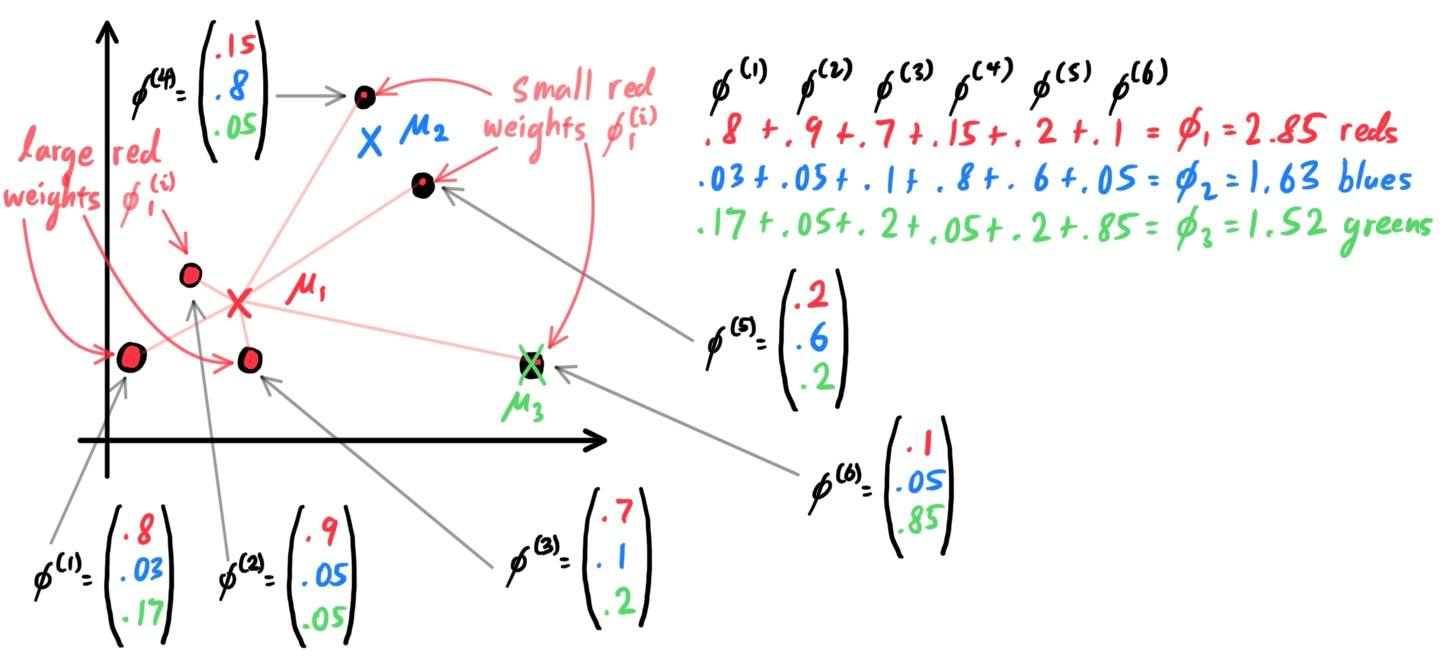
\includegraphics[scale=0.27]{img/weighted_means.jpg}
            \caption{} 
            \label{fig:weighted_means}
          \end{figure}

          With this logic of weighted points, we finally update the covariance matrices $\Sigma_j$ as below:
          \[\Sigma_j = \frac{1}{\sum_{i=1}^n \phi_j^{(i)}} \sum_{i=1}^n \phi^{(i)}_j \,\big(x^{(i)} - \mu_j\big)\big(x^{(i)} - \mu_j\big)^T\]

          \item Now, we have new values of $\phi, \mu_1, \ldots, \mu_k, \Sigma_1, \ldots, \Sigma_k$ that we can work with. With these new values, repeat steps 2 and 3 until convergence.
        \end{enumerate}

        All in all, this entire algorithm results from modifying the "hard" data of each point $x^{(i)}$ being undoubtedly in one cluster to a model containing points $x^{(i)}$ that have been "smeared" around different clusters, with a probability $\phi_j^{(i)}$ being in cluster $j$. 
      \end{definition}

      \begin{definition}[Mixture of Gaussians Algorithm: Summary]
        Given a training set $\{x^{(i)}\}_{i=1}^n \in \mathbb{R}^d$, let us assume that the random variable $X$ that these examples follow can be modeled by specifying a joint distribution of a multinomial and Gaussians. 
        That is, it follows a Gaussian mixture model (GMM) of $k$ Gaussian clusters. Let
        \begin{itemize}
          \item $Z$ be the multinomial distribution representing which Gaussian cluster each example $x$ falls in, with density represented by vector $\phi \in \mathbb{R}^k$ so that $\mathbb{P}(Z = j) \equiv \phi_j$.
          \item The set of conditional distributions 
            \[X\,|\,Z = j \sim \mathcal{N}(\mu_j, \Sigma_j) \text{ for } j = 1, 2, \ldots, k\]
          are multivariate Gaussian, with mean vectors $\mu_1, \ldots, \mu_k$ and covariance matrices $\Sigma_1, \ldots, \Sigma_k$. 
        \end{itemize}
        Let all the parameters be denoted as $\theta$. Then, the EM algorithm is as such: 
        \begin{enumerate}
          \item Initialize the multinomial vector $\phi$, the $\mu_j$'s, and the $\Sigma_j$'s.
          \item \textbf{(E Step)} Calculate the $n$ vectors
            \[\phi^{(i)} = \begin{pmatrix} \phi_1^{(i)} \\ \vdots \\ \phi_k^{(i)} \end{pmatrix} \text{ for all } i = 1, \ldots, n\]
          that represent the posterior distribution of $Z$ given observed $x^{(i)}$ by computing 
            \begin{align*} 
              \phi_j^{(i)} & = p_Z^{(i)} \big(z = j;\, \phi, \mathbf{\mu}, \mathbf{\Sigma} \big) \\
              & = p_Z \big(z = j\,|\, x^{(i)}; \, \phi, \mathbf{\mu}, \mathbf{\Sigma} \big) \\
              & = \frac{p_{\mathcal{N}_j} \big(x^{(i)}\,|\,z^{(i)} = j; \, \mathbf{\mu}, \mathbf{\Sigma}\big) \; p_Z \big(z^{(i)} = j;\, \phi \big)}{p_X \big(x^{(i)};\, \phi, \mathbf{\mu}, \mathbf{\Sigma}\big)} \\
              & = \frac{p_{\mathcal{N}_j} \big(x^{(i)}\,|\,z^{(i)} = j; \, \mathbf{\mu}, \mathbf{\Sigma}\big) \; p_Z \big(z^{(i)} = j;\, \phi \big)}{\sum_{l=1}^k p_{\mathcal{N}_j} \big( x^{(i)}\,|\, z^{(i)} = l;\, \mathbf{\mu}, \mathbf{\Sigma} \big)\; p_Z \big(z^{(i)} = l; \,\phi\big)}
            \end{align*}
          \item \textbf{(M Step)} Reassign the value of $\theta$ as 
            \begin{align*} 
              \phi & = \frac{1}{n} \sum_{i=1}^n \phi^{(i)} \\
              \mu_j & = \frac{\sum_{i=1}^n \phi_j^{(i)} x^{(i)}}{\sum_{i=1}^n w_j^{(i)}} \text{ for } j = 1, \ldots, n \\
              \Sigma_j & = \frac{1}{\sum_{i=1}^n \phi_j^{(i)}} \sum_{i=1}^n \phi^{(i)}_j \, \big(x^{(i)} - \mu_j \big) \big(x^{(i)} - \mu_j\big)^T \text{ for } j = 1, \ldots, n 
            \end{align*}
          \item Repeat steps 2 and 3 until convergence.
        \end{enumerate}
      \end{definition}

    \subsubsection{EM Algorithm for General Estimation Problems}

      Recall \textbf{Jensen's Inequality}: Given a convex function $f: \mathbb{R} \longrightarrow \mathbb{R}$ (meaning that $f^{\prime\prime} (x) \geq 0$ for all $x$) and a random variable $X$, we have 
      \[\mathbb{E}\big(f(X)\big) \geq f\big(\mathbb{E}(X)\big) \]
      Moreover, if $f$ is strictly convex, then $\mathbb{E}\big( f(X)\big) = f\big(\mathbb{E}(X)\big)$ holds true if and only if $X = \mathbb{E}(X)$ with probability $1$ (i.e. if $X$ is a constant). 

      Suppose we have an estimation problem given the training set $\{x^{(i)}\}_{i=1}^n$. We have latent variable model $p(x, z; \theta)$ with $z$ being the latent variable of discrete, finite random variable $Z$, with density $p_Z (z)$. Let us denote the density of $X$ as $p_X$. Then, the random variable $X$ can be interpreted as us first generating $z$ from $Z$, and then computing $X\,|\,Z = z$.  
      \[\text{Compute } X = \text{Compute } Z \text{ and then } \begin{cases} 
      \text{Compute } X \,|\, Z = 1 \\
      \text{Compute } X \,|\, Z = 2 \\
      \ldots \\
      \text{Compute } X \,|\, Z = k
      \end{cases}\]

      Let us clarify some notation: 
      \begin{itemize}
        \item The distribution that we will iteratively reassign over and over again is $Z$, with density $p_Z$ that maps $z \mapsto \phi_z$, where $\phi$ is a vector that represents the density.
        \item The $k$ conditional (not necessarily Gaussian) distributions that we will iteratively reassign over and over again is $X_1, X_2, \ldots, X_k$, with densities $p_{X_1} (x), \ldots, p_{X_k} (x)$ that maps $x \mapsto p_{X_j} (x)$.
        \item The distribution of the entire random variable $X$ will have density $p_X (x)$. Since we are iteratively reassigning the densities $p_Z$ and $p_{X_j}$, this joint distribution of $X$ will also get modified.
      \end{itemize}

      The EM algorithm in the general case has the following steps: 
      \begin{enumerate}
        \item We initialize the value of $\theta$ in some way. Note that within this $\theta$ are the parametizations of the initial multinomial density $p_Z$, which is our initial "guess" of the distribution of $Z$.
        \item \textbf{(E Step)} The log likelihood of the given data $\{ x^{(i)}\}_{i=1}^n$ with respect to the parameter $\theta$ (which encodes all parameters of distribution $Z$ and all $X\,|\,Z$) is 
          \[l(\theta) = \sum_{i=1}^n \log\, p_X \big( x^{(i)}; \, \theta \big)\]
        It turns out that explicitly finding the maximum likelihood estimates of the parameters $\theta$ is hard because it results in a difficult, non-convex optimization problem. So, we tackle this another way. 
        
        To start, we can see that the summation isn't too crucial, so we can focus on minimizing each $\log \, p_X \big(x^{(i)}; \, \theta \big)$ and summing in the end. We can calculate this by conditioning over all $j = 1, \ldots, k$ generated from $Z$ (which we have guessed to have an initial density of $p_Z$). That is, we must find for each $i = 1, 2, \ldots, n$ 
        \begin{align*} 
          \max_\theta \log \, p_X \big( x^{(i)}; \, \theta \big) & = \max_\theta \log \, \bigg(\sum_{j=1}^k p_X \big(x^{(i)}, Z = j; \, \theta\big) \bigg) \\
          & = \max_\theta \log \bigg( \sum_{j=1}^k p_X \big( x^{(i)}\,|\, Z = j; \, \theta\big) p_Z \big( j; \, \theta \big) \bigg) \\
          & = \max_\theta \log \bigg( \sum_{j=1}^k p_{X_j} \big( x^{(i)} ;\, \theta\big) p_Z \big( j; \, \theta \big) \bigg)
        \end{align*}
        To find this maximum value, we can focus on the first equality and see that by Jensen's inequality (with conCAVE, not convex, $f(x) = \log x$ over domain $x \in \mathbb{R}^+$), the following holds true for all $\theta$ and more importantly, for \textit{any arbitrary density function} $p_Z^{*i}$.  
        \begin{align*} 
          \log p_X \big(x^{(i)};\, \theta\big) & = \log \bigg( \sum_{j=1}^k p_X \big(x^{(i)}, Z = j;\, \theta \big) \bigg) \\ 
          & = \log \bigg( \sum_{j=1}^k p_Z^{*i} \big(j \big)\, \frac{p_X \big(x^{(i)}, Z = j;\, \theta \big)}{p_Z^{*i} \big(j \big)} \bigg) \\
          & = \log \Bigg(\mathbb{E}_{j \sim p_Z^{*i}} \bigg( \frac{p(x^{(i)}, Z = j; \, \theta)}{p_Z^{*i} \big(j \big)}\bigg)\Bigg) \\
          & \geq \mathbb{E}_{j \sim p_Z^{*i}} \Bigg( \log \bigg( \frac{p(x^{(i)}, Z = j; \, \theta)}{p_Z^{*i} \big(j \big)} \bigg) \Bigg) \\
          & = \sum_{j=1}^k p_Z^{*i} (j) \, \log\bigg( \frac{p(x^{(i)}, Z = j; \, \theta)}{p_Z^{*i} (j)} \bigg) = \text{ELBO} \big( x^{(i)}; \,p_Z^{*i}, \theta \big)
        \end{align*}
        The final term, called the \textbf{evidence lower bound} (ELBO), is just the expectation of $\log \frac{p(x^{(i)}, Z = j; \, \theta)}{p_Z^{*i} (j)}$ with respect to $j$ drawn from density $p_Z^{*i}$, which is denoted with $\mathbb{E}_{j \sim p_Z^{*i}}$. 
        
        Summing over all $n$ examples, we have a lower bound for the entire log likelihood for \textit{any} set of density functions $p_Z^{*1}, p_Z^{*2}, \ldots, p_Z^{*n}$: 
        \begin{align*} 
          l(\theta) = \sum_{i=1}^n \log p(x^{(i)}; \, \theta) & \geq \sum_{i=1}^n \text{ELBO}(x^{(i)}; \, p_Z^{*i}, \theta) \\
          & = \sum_{i=1}^n \sum_{j=1}^k p_Z^{*i} (j) \, \log\bigg( \frac{p(x^{(i)}, Z = j; \, \theta)}{p_Z^{*i} (j)} \bigg)
        \end{align*}
        Our job now is to choose the correct density functions $p_Z^{*i}$'s such that the lower bound is maximized. It turns out that we can do even better: equality is satisfied if and only if we set 
        \begin{align*} 
          p_Z^{*i} (j) & \equiv p_Z \big( j\,|\, x^{(i)}; \, \theta \big) \\
          & \equiv p_Z^{(i)} \big( j; \, \theta \big) \text{ for all } i = 1, 2, \ldots, n
        \end{align*}
        which is simply the posterior distribution of the multinomial given the observed sample $x^{(i)}$, which we can easily calculate using Bayes' rule. Substituting this into $p_Z^{*i}$ leads to the equality 
        \begin{align*} 
          l(\theta) = \sum_{i=1}^n \log p (x^{(i)}; \, \theta) 
          & = \sum_{i=1}^n \text{ELBO}\big(x^{(i)}; p_Z^{(i)}, \, \theta \big) \\
          & = \sum_{i=1}^n \sum_{j=1}^k p_Z^{(i)} \big( j; \, \theta \big) \, \log\bigg( \frac{p(x^{(i)}, Z = j; \, \theta)}{p_Z^{(i)} \big( j; \, \theta \big)} \bigg) \\
          & = \sum_{i=1}^n \sum_{j=1}^k p_Z \big( j\,|\, x^{(i)}; \, \theta \big) \, \log\bigg( \frac{p(x^{(i)}, Z = j; \, \theta)}{p_Z \big( j\,|\, x^{(i)}; \, \theta \big)} \bigg)
        \end{align*}
        In summary, this E step has taken the log-likelihood function $l(\theta)$ (representing (the log of) the probability of all the $x^{(i)}$'s landing where they are given the parameters $\theta$), which is abstract and hard-to-optimize, and converted it into an equivalent form as the sum of a bunch of ELBO functions optimized with the density parameters begin assigned $p_Z^{*i} = p_Z^{(i)}$. 
        
        But remember that these optimal densities $p_Z^{*i} = p_Z^{(i)}$ make the right and left hand side equivalent only for a \textbf{fixed value} of $\theta$! So, the right hand side is only equivalent to $l(\theta)$ only for that one value of $\theta$, but as soon as we set $\theta$ to something else, the right hand side evaluated with $p_Z^{*i} = p_Z^{(i)}$ are not equal.
        \item \textbf{(M Step)} Since we have found some equivalent form of $l(\theta)$ for the fixed $\theta$ that was initialized, we can now just maximize the right hand side with respect to $\theta$, while fixing the $p_Z^{*i} = p_Z^{(i)}$'s. Therefore, we find and set the value of $\theta$ as 
        \begin{align*}  
          \theta & = \text{arg}\; \max_\theta \sum_{i=1}^n \text{ELBO} \big( x^{(i)}; \, p_Z^{(i)}, \theta \big) \\
          & = \text{arg}\; \max_\theta \sum_{i=1}^n \sum_{j=1}^k p_Z^{(i)} (j)\; \log \bigg( \frac{p(x^{(i)}, Z = j; \, \theta)}{p_Z^{(i)} (j)} \bigg) \\
          & = \text{arg}\; \max_\theta \sum_{i=1}^n \sum_{j = 1}^k p_Z \big(j\,|\, x^{(i)}; \, \theta \big)\, \log \bigg( \frac{p(x^{(i)}, Z = j; \, \theta)}{p_Z \big(j\,|\, x^{(i)}; \, \theta \big)} \bigg)
        \end{align*}
        In the case where the parameter $\theta$ consist of $\phi, \mu_1, \ldots, \mu_k, \Sigma_1, \ldots, \Sigma_k$ like in the GMM model, it happens so that the maximum is found by computing $\phi$ to be the average of the $\phi^{(i)}$'s, each $\mu_j$ to be the weighed averages of the points, and each $\Sigma_j$ as the equation above. For other distributions, the formula for the maximum must be mathematically found (or algorithmically computed) with respect to parameter $\theta$.
        \item We have now reassigned the entire value of $\theta$, meaning that the parameters representing our guess of density $p_Z$ of $Z$ has also been modified. With this new value of $\theta$, we repeat steps 2 and 3 until convergence.
      \end{enumerate}

      For some intuition, we can visualize $l$ as a function of $\theta$. For the sake of visuals, we will assume that $\theta \in \mathbb{R}$ and $l: \mathbb{R} \longrightarrow \mathbb{R}$. On the contrary to what a visual is supposed to do, we want to point out that we cannot just visualize $l$ as a curve in $\mathbb{R} \times \mathbb{R}$. This can be misleading since then it implies that the optimal $\theta$ value is easy to find, as shown in the left. Rather, we have no clue what the whole curve of $l$ looks like, but we can get little snippets (right). 

      \begin{figure}[H]
        \centering 
        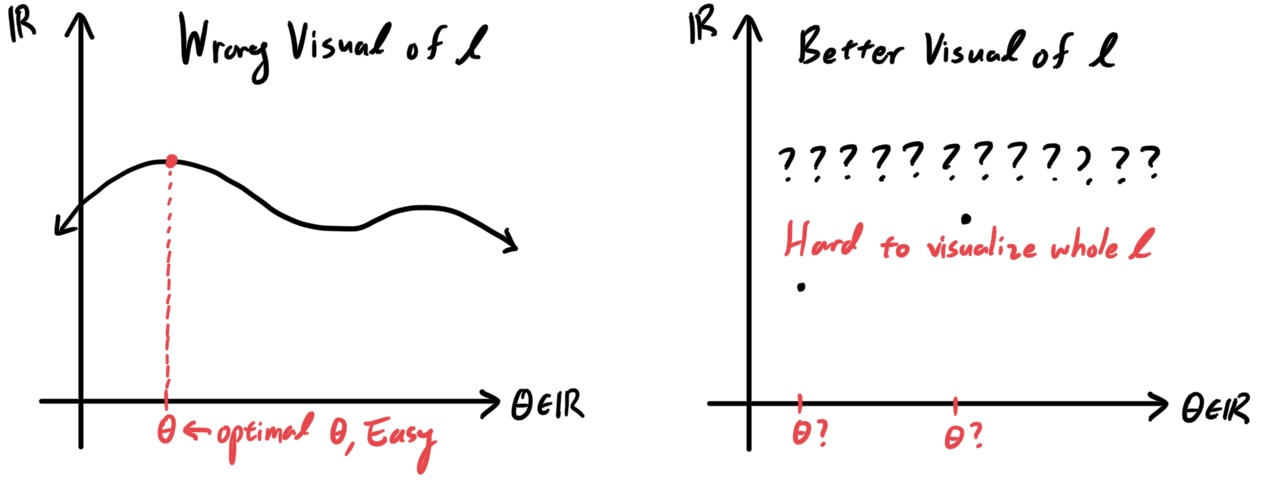
\includegraphics[width=0.6\textwidth]{img/visual_of_l.jpg}
        \caption{} 
        \label{fig:visual_of_l}
      \end{figure}

      Rather, all we can do is hope to take whatever easier-to-visualize, lower-bound functions and maximize them as much as we can in hopes of converging onto $l$. Let us walk through the first two iterations of the EM algorithm. We first initialize $\theta$ to, say $\theta_0$. This immediately induces the lower-bound ELBO-sum function $\sum_{i} \text{ELBO} (x^{(i)};\, p_Z^{*i}, \theta)$, which takes in multinomial density functions $p_Z^{*i} = p_1, p_2, \ldots$ and outputs different functions of $\theta$ that are valid lower bounds. Two of these possible lower-bound functions are shown (in green) for when we input some arbitrary density $p_1, p_2$. However, there exists a density $p_Z^{(i)}$ that produces not only the maximum possible lower-bound (called max ELBO, shown in red) but is equal to $l(\theta)$ for that density input $p_Z^{(i)}$. We maximize this function with respect to $\theta$ to get $\theta_1$ as our next assignment of $\theta$. 

      \begin{figure}[H]
        \centering 
        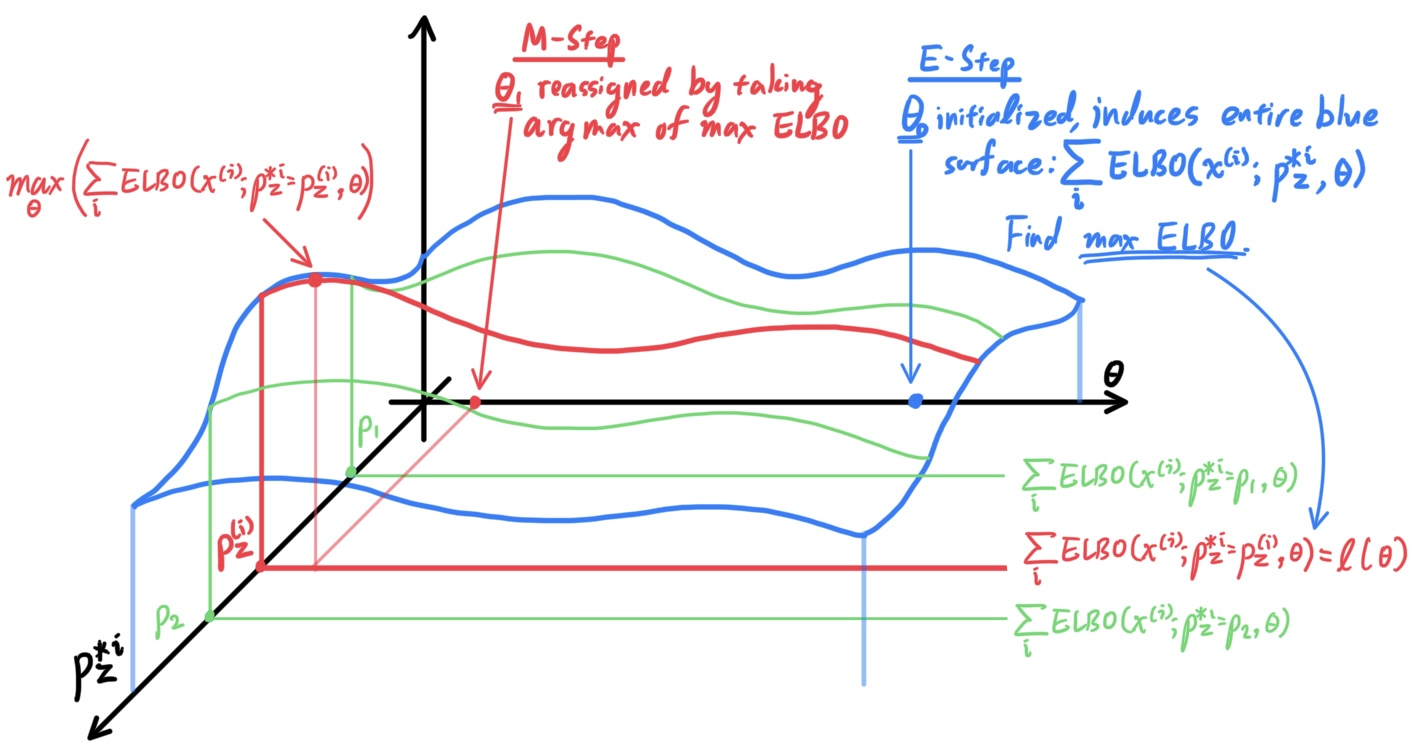
\includegraphics[width=0.7\textwidth]{img/EM_first_iteration.jpg}
        \caption{} 
        \label{fig:EM_first_iteration}
      \end{figure}

      The next step is identical. Now that we have a new value of $\theta = \theta_1$, this induces the lower-bound ELBO-sum function $\sum_{i} \text{ELBO} (x^{(i)};\, p_Z^{*i}, \theta)$ that also takes in multinomial densities $p_Z^{*i}$ and outputs different functions of $\theta$ that are valid lower-bounds. Two possible lower bounds are shown (in green), but the maximum lower-bound (in blue) is produced when we input density $p_Z^{(i)}$. Since this max ELBO function is equal to $\theta$ for this fixed density input $p_Z^{(i)}$, we maximize this function with respect to $\theta$ to get $\theta_2$ as our next assignment of $\theta$. 

      \begin{figure}[H]
        \centering 
        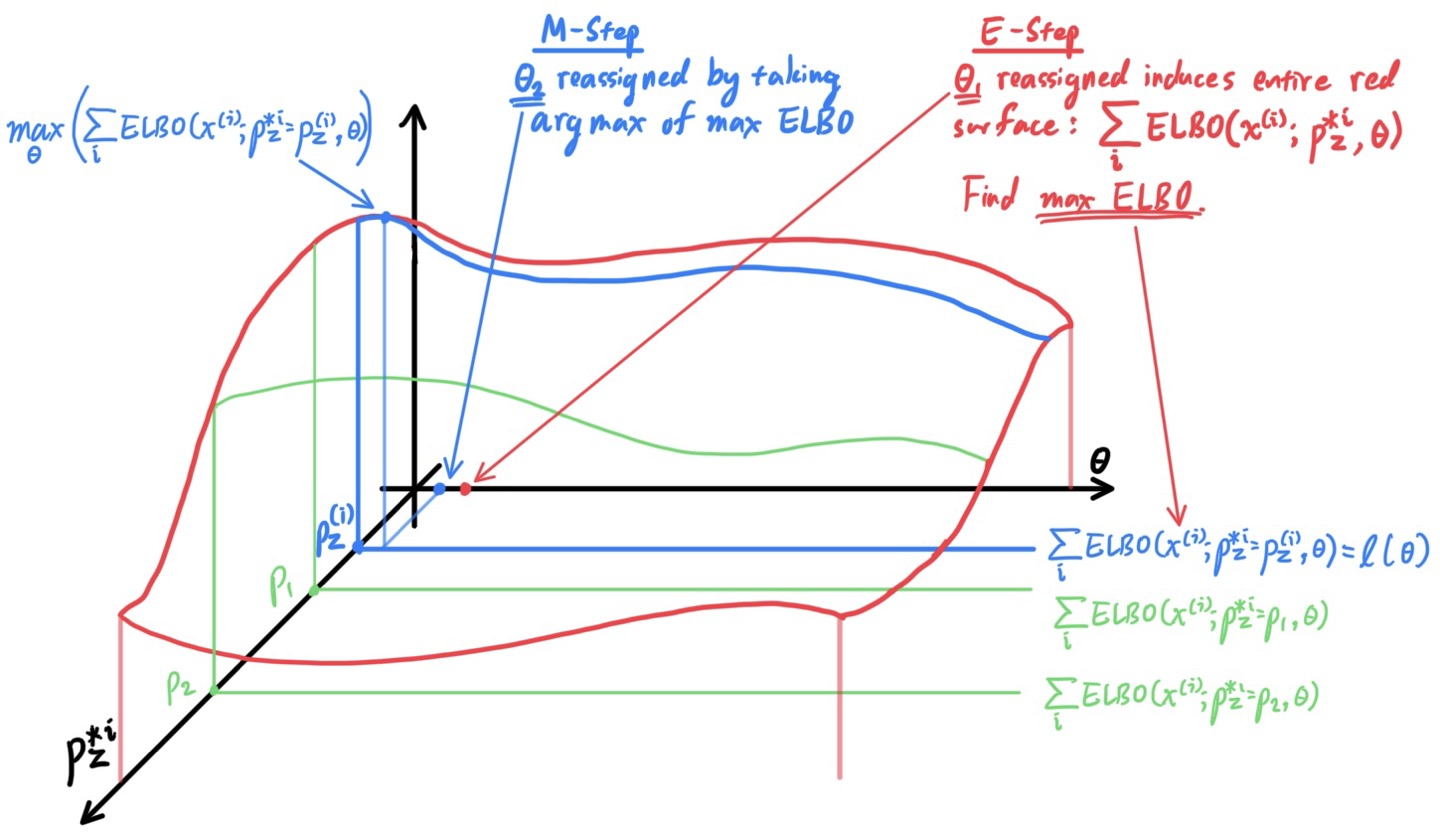
\includegraphics[width=0.7\textwidth]{img/EM_second_iteration.jpg}
        \caption{} 
        \label{fig:EM_second_iteration}
      \end{figure}

      \begin{definition}[EM Algorithm for General Estimation Problems]
        Given a training set $\{x^{(i)}\}_{i=1}^n \in \mathbb{R}^d$, let us assume that the random variable $X$ that these examples follow can be modeled by specifying a joint distribution of a multinomial and some arbitrary distributions. Let there be $k$ clusters, and let 
        \begin{itemize}
          \item $Z$ be the multinomial distribution representing which Gaussian cluster each example $x$ falls in, with density $p_Z (j)$ and represented by vector $\phi \in \mathbb{R}^k$ so that $\mathbb{P}(Z = j) = \phi_j$. Let the parameters of $\phi$ be encoded in $\theta$.
          \item The set of conditional distributions
            \[X\,|\,Z = j \sim X_j \text{ for } j = 1, 2, \ldots, k\]
          are arbitrary distributions with some parameters, also all encoded in $\theta$.  
        \end{itemize}

        The EM algorithm is described as such: 
        \begin{enumerate}
          \item Initialize $\theta$.
          \item \textbf{(E Step)} Since $l(\theta)$ is bounded below for all $p_Z^{*1}, \ldots, p_Z^{*n}$ as 
            \[l(\theta) \equiv \sum_{i=1}^n \log p\big( x^{(i)}; \, \theta\big) \geq \sum_{i=1}^n \text{ELBO}\big( x^{(i)}; \, p_Z^{*i}, \theta\big)\]
          setting $p_Z^{*i} (j) = p_Z^{(i)} (j) = p_Z \big(j\,|\, x^{(i)}; \, \theta\big)$ for all $i = 1, \ldots, n$ would put $l$ into a new form for these specific fixed values of $p_Z^{*i}$. 
            \[l(\theta) = \sum_{i=1}^n \text{ELBO}\big(x^{(i)}; p_Z^{(i)}, \theta \big)\]
          \item \textbf{(M Step)} We maximize this equivalent form of $l(\theta)$ with respect to $\theta$ whilst fixing the choice of $p_Z^{(i)}$. That is, we set the value of $\theta$ as 
          \begin{align*}  
            \theta & = \text{arg}\; \max_\theta \sum_{i=1}^n \text{ELBO} \big( x^{(i)}; \, p_Z^{(i)}, \theta \big) \\
            & = \text{arg}\; \max_\theta \sum_{i=1}^n \sum_{j=1}^k p_Z^{(i)} (j)\; \log \bigg( \frac{p(x^{(i)}, Z = j; \, \theta)}{p_Z^{(i)} (j)} \bigg) \\
            & = \text{arg}\; \max_\theta \sum_{i=1}^n \sum_{j = 1}^k p_Z \big(j\,|\, x^{(i)}; \, \theta \big)\, \log \bigg( \frac{p(x^{(i)}, Z = j; \, \theta)}{p_Z \big(j\,|\, x^{(i)}; \, \theta \big)} \bigg)
          \end{align*}
          \item We have successfully updated $\theta$. Now, we repeat steps 2 and 3 until convergence. Step 2 can bring improvements because we have changed the $\theta$, which means that there is a new sum of ELBO functions of the $\theta$ that serves as a new lower bound.
        \end{enumerate}
      \end{definition}
  \subsection{Kernel Density Estimation} 

  \subsection{Density Based Clustering}

  \subsection{Hierarchical Clustering} 

  \subsection{Spectral Clustering}

  \subsection{High Dimensional Clustering}

\section{Graphical Models} 

  \subsection{Bayesian Networks} 

  \subsection{Markov Random Fields}

  \subsection{Hidden Markov Models}

\section{Dimensionality Reduction} 

  Dimensionality reduction is used for many purposes, such as preprocessing data, visualizing it, or encoding it in a sparser, more efficient way. 

  \subsection{Principal Component Analysis} 
    
    PCA finds low dimensional approximations to the data by projecting the data onto linear subspaces. 

    \begin{definition}[Principal Component Analysis]
      Let $X \in \mathbb{R}^d$ and $\mathcal{L}_k$ denote all $k$-dimensional linear subspaces. The $k$th principal subspace is 
      \begin{equation}
        \ell_k = \argmin_{\ell \in \mathcal{L}_k} \mathbb{E} \big( \min_{y \in \ell} ||\Tilde{X} - y||^2 \big)
      \end{equation}
      where $\Tilde{X} = X - \mu$ and $\mu = \mathbb{E}[X]$. To parse this, let's fix a subspace $\ell$. Then, the normalized data $\Tilde{X}$ is a random vector and the minimum distance of $\Tilde{X}$ onto the subspace $\ell$ is the inner min term. Taking the expectation of that gives us the expected distance of the data onto the subspace. The principal subspace is the subspace that minimizes this expected distance. The dimension reduced version of $X$ is then $T_k (X) = \mu + \mathrm{proj}_{\ell_k} X$. 
    \end{definition}

    Note that this is in fact different from linear regression as it minimizes the expected \textit{orthogonal distance} to the subspace, rather than the residual distance to the subspace as in linear regression. 

    \begin{figure}[H]
      \centering
      \begin{subfigure}[b]{0.3\textwidth}
      \centering
        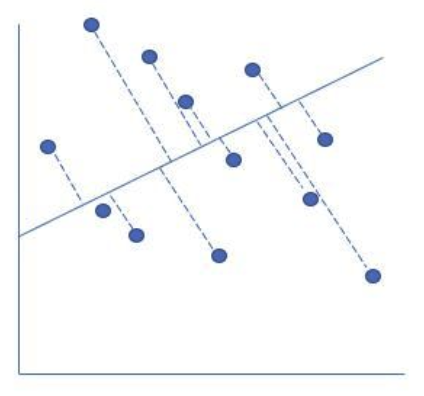
\includegraphics[width=\textwidth]{img/pca_ortho.png}
        \caption{PCA minimizes the orthogonal distance to the subspace. }
      \end{subfigure}
      \begin{subfigure}[b]{0.3\textwidth}
      \centering
        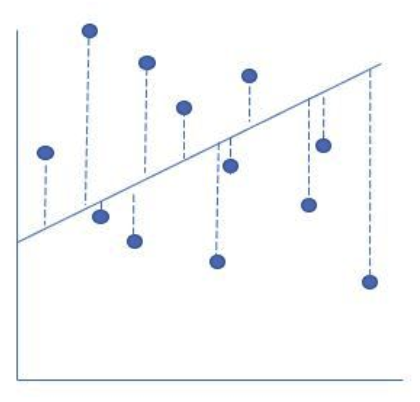
\includegraphics[width=\textwidth]{img/lin_reg_vert.png}
        \caption{Linear regression minimizes the residual distance to the subspace.} 
      \end{subfigure}
      \caption{PCA vs Linear Regression}
      \label{fig:pca_lin_reg}
    \end{figure}

    There is a very nice way to calculate this principal subspace. 

    \begin{theorem}[Calculating the Principal Subspace] 
      Given our data matrix $X \in \mathbb{R}^{n \times d}$, we take the SVD of it. 
      \begin{equation}
        X = U \Sigma V^T
      \end{equation}
      where $\Sigma$ contains the singular values of $X$ in decreasing order. Then $\ell_k$ is the subspace spanned by the columns $v_1, v_2, \ldots, v_k$ of $V$. Furthermore, 
      \begin{equation}
        T_k (X) = \mu + \sum_{j=1}^k \beta_j v_j , \text{ where } \beta_j = \langle X - \mu, v_j \rangle
      \end{equation}
      Note that this is really just equivalent to calculating the eigendecomposition of $\hat{\Sigma} = X^T X$. 
    \end{theorem}

    Now a question arises: how do we know that this sample decomposition is a good approximation to the true decomposition? It comes from the fact that the sample covariance $\hat{\Sigma}$ is a good approximation of the true covariance $\Sigma$, which we will later prove using concentration of measure. 

    \begin{theorem}[Risk]
      The risk satisfies 
      \begin{equation}
        R(k) = \mathbb{E}[|| X - T_k (X) ||^2 ] = \sum_{j=k+1}^d \lambda_j 
      \end{equation}
    \end{theorem}

    It is essential that you plot the spectrum in decreasing order. This allows you to analze how well PCA is working. People often use the ``elbow'' technique to determine where to choose $K$, and we value 
    \begin{equation}
      \frac{\sum_{j=1}^k \lambda_j}{\sum_{j=1}^d \lambda_j} 
    \end{equation}
    accounts for the \textbf{variance explained}, which should be high with $K$ low. If you have to go out to dimension $K=50$ to explain $90\%$ of the variance, then PCA is not working. It may not work because of many reasons, such as there being nonlinear structure within the data. 

    It turns out that the elements of $\hat{\Sigma}$ are close entry-wise to those of $\Sigma$. But if this is true, then does it mean that the eigenvalues of the sample covariance matrix are close to the true eigenvalues of the covariance matrix? It turns out that the answer is no, and we need a proper metric to satisfy this assumption. The metric, as we can guess from linear algebra, is the operator norm, and we will show some results from matrix perturbation theory. 

    \begin{definition}[Operator Norm]
      The \textbf{operator norm} of a matrix $A$ is defined as 
      \begin{equation}
        ||A|| = \sup_{x \neq 0} \frac{||Ax||}{||x||} 
      \end{equation}
    \end{definition}

    \begin{lemma}[]
      It turns out that 
      \begin{equation}
        ||\hat{\Sigma} - \Sigma|| = O_p \bigg( \frac{1}{\sqrt{n}} \bigg)
      \end{equation}
    \end{lemma}

    \begin{theorem}[Weyl's Theorem]
      If $\hat{\Sigma}$ and $\Sigma$ are close in the operator norm, then their eigenvalues are close. 
      \begin{equation}
        ||\hat{\Sigma} - \Sigma|| = O_p \bigg( \frac{1}{\sqrt{n}} \bigg) \implies |\hat{\lambda}_j - \lambda_j| = O_p \bigg( \frac{1}{\sqrt{n}} \bigg) 
      \end{equation}
    \end{theorem}

    This only talks about their eigenvalues, but this does not necessarily imply that the eigenvalues are close. We need an extra condition. 

    \begin{theorem}[David-Kahan Theorem]
      If $\hat{\Sigma}$ and $\Sigma$ are close in the operator norm, and if the eigenvectors of $\Sigma$ are well-conditioned, then the eigenvectors of $\hat{\Sigma}$ are close to the eigenvectors of $\Sigma$. More specifically, 
      \begin{equation}
        ||\hat{v}_j - v_j|| \leq \frac{2^{3/2} ||\hat{\Sigma} - \Sigma||}{\lambda_j - \lambda_{j+1}}
      \end{equation}
    \end{theorem}

    \subsubsection{Kernel PCA}

      \begin{definition}[Kernel PCA]
        Let $N_i$ be the neighborhood around $X_i$. Then, we want to find a mapping $W: \mathbb{R}^n \rightarrow \mathbb{R}^k$ that minimizes 
        \begin{equation}
          \min_{W} \sum_{i=1}^n \bigg| \bigg| X_i - \sum_{j \in N_i} W_{ij} X_j \bigg| \bigg|^2 \text{ where } \sum_{j} W_{ij} = 1
        \end{equation}
        We can constrain the weights in $W$ so that anything that is not in the neighborhoods are $0$. 
      \end{definition}

  \subsection{Multi-Dimensional Scaling}

    Again, we want to reduce our dimension, but the goal is slightly different from PCA. 

    \begin{definition}[Multi-Dimensional Scaling]
      Given our data $X \in \mathbb{R}^d$, we want to construct a linear map $T: \mathbb{R}^d \rightarrow \mathbb{R}^k$ such that it preserves the pairwise differences between the data points. That is, we want to minimize the following loss function 
      \begin{equation}
        \min_{T} \sum_{i \neq j} \big( d_{\mathbb{R}^k}(T(x_i), T(x_j)) - d_{\mathbb{R}^d}(x_i, x_j) \big)
      \end{equation}
      where $d_{V}$ is a distance metric in the space $V$. 
    \end{definition}

    Note that we can easily modify this formulation to preserve other structures, such as dot products, weights between distances, or different types of metrics in each space. It turns out that when the distance metric is the Euclidean L2 distance, then the solution to this linear map turns out to be PCA. This may be a more intuitive way to think about PCA, since we're trying to preserve the pairwise distances between the data points. 

    \begin{theorem}[Equivalence of Classical MDS and PCA]
      If the distance metric is the Euclidean L2 distance, then the solution to the MDS problem is equivalent to PCA. That is, 
      \begin{equation}
        T_k = \argmin_{T} \sum_{i \neq j} \big( ||T(x_i) - T(x_j)||^2 - ||x_i - x_j||^2 \big)
      \end{equation}
    \end{theorem}

    Generally, if you don't use classical MDS, then you will get a different answer than PCA and there doesn't exist a closed form solution, so you'll have to minimize this numerically. 

    \begin{example}[Non Classical MDS]
      The loss 
      \begin{equation}
        \sum_{i \neq j}  \big( ||T(x_i) - T(x_j)|| - ||x_i - x_j|| \big)^2 
      \end{equation}
      does not give the same solution as PCA. 
    \end{example}

    \subsubsection{Isomap} 

      Isomap is a bit different in the way that it tries to capture more of the global structure of the data, which brings advantages and disadvantages. It is simply a modification of MDS but with geodesic distances. 

      \begin{definition}[Isomap]
        You start off with the point cloud, but with every point, $X_i$, you find the local neighborhood $N_i$ and you make a weighted graph over the whole dataset in the high dimensional space. Then, the distance between any two arbitrary points is the weighted sum of the path between them, calculated by Dijkstra's algorithm. Intuitively, this is an approximation of the geodesic distance between these two points on a manifold. Call this distance $d_G$. Then, we simply do MDS by minimizing 
        \begin{equation}
          \min_{T} \sum_{i \neq j} \big( d_{\mathbb{R}^k}(T(x_i), T(x_j)) - d_G(x_i, x_j) \big)
        \end{equation}

        \begin{figure}[H]
          \centering 
          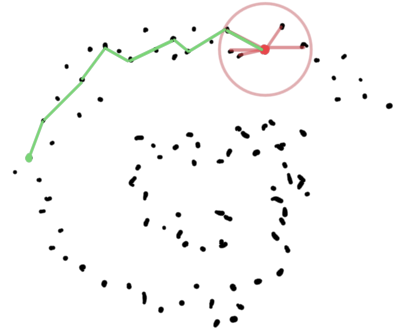
\includegraphics[scale=0.4]{img/isomap.png}
          \caption{The classical example is the spiral manifold. The data lies in this manifold, and the geodesic distance helps us gain an accurate distance metric within this data. } 
          \label{fig:isomap}
        \end{figure}
      \end{definition}

      The problem with this is that it is very sensitive to noise. For example, if we had a few points lying between the spirals, then the geodesic distance between the two spirals would be very small, and so the MDS would try to bring them closer together.  

      \begin{figure}[H]
        \centering 
        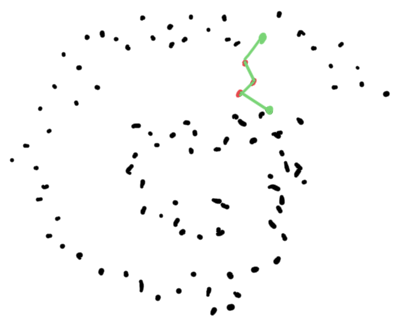
\includegraphics[scale=0.4]{img/isomap_problem.png}
        \caption{With extra noisy points (red), the geodesic distance can get corrupted.} 
        \label{fig:isomap_problem}
      \end{figure}

      To fix this, we use \textit{diffusion maps}, which looks at all possible paths between two points and looks at some average of them, which increases robustness. 

  \subsection{Local Linear Embedding} 

    PCA and MDS are linear embedding methods. Let's move onto nonlinear ones. The first nonlinear models that we work with again use the idea of locality (remember kernel regression). You have data that is globally nonlinear, but if you look at a point and its local neighborhood around it, then it is approximately linear since we assume that it lives in some smooth manifold. 

    \begin{figure}[H]
      \centering 
      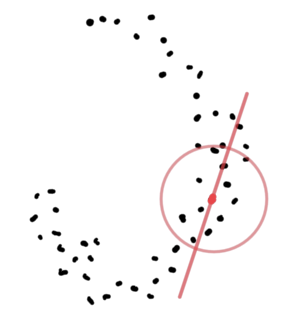
\includegraphics[scale=0.4]{img/local_linear_embedding.png}
      \caption{Local linear embedding assumes that the data is locally linear. } 
      \label{fig:local_linear_embedding}
    \end{figure}

    The concept of neighborhood can be defined in two ways. You can either just fix an $\epsilon$ and take the $\epsilon$-ball around each point $x_i$. Or you can fix a $k$ and take the $k$ nearest neighbors of each point. The general idea of using kernel PCA is to take a local neighborhood of the data and construct some linear approximation of it. 

  \subsection{Factor Analysis}

    Factor analysis is very similar to PCA since it looks for a small number of hidden features within the data. Say that we want to do density estimation for the probability distribution of the covariates $\mathbf{x}$, a random variable. We can try to model it directly, but this may be infeasible. Rather, what we do is ``add" a latent distribution $\mathbf{h}$, creating the joint distribution $(\mathbf{x}, \mathbf{h})$. This may look more complicated, but make two simplifying assumptions: we hope that we can model the latent $\mathbf{h}$ in a simple form (like a Gaussian), and we can model the conditional probability $p(\mathbf{x} \mid \mathbf{h})$ as some function $f_\theta$ parameterized by $\theta$. We can therefore marginalize and find that 
    \begin{equation} 
      p(\mathbf{x}) = \int p(\mathbf{x} \mid \mathbf{h}) \, p(\mathbf{h}) \,d\mathbf{h} = \mathbb{E}_\mathbf{h} [p(\mathbf{x} \mid \mathbf{h})] 
    \end{equation}

    Like we do with everything else in math, we take a look at the simplest example: linear functions. 

    In \text{linear factor models}, we start with the unknown covariate distribution $\mathbf{x} \in \mathbb{R}^d$, and we create a latent variable $\mathbf{h} \in \mathbb{R}^k$ ($k$ is to be chosen). We first assume that 
    \[\mathbf{h} \sim p(\mathbf{h})\] 
    comes from some predefined distribution, with the only constraint being that it is factorable (i.e. is the product of its marginal distributions: $p(\mathbf{h}) = \prod_i p(h_i)$) so that it is easy to sample from. Occasionally, the stronger assumption of the $h_i$'s being iid is made. Then, we assume that 
    \[\mathbf{x} = \mathbf{W} \mathbf{h} + \mathbf{b} + \epsilon\] 
    where the noise $\epsilon$ is typically Gaussian and diagonal (but not necessarily the same component-wise variances). Finally, we can use techniques like MLE to estimate $\mathbf{W}, \mathbf{b}$, and the parameters of $\epsilon$.  

    The entire reason we want to do this is that we are hoping that $\mathbf{h} \in \mathbb{R}^k$ and $\mathbf{x} \in \mathbb{R}^d$, and $d >> k$. Therefore, $\mathbf{W}$ is a $d \times k$ matrix, and the latent variables $\mathbf{h}$ give a more compact (parsimonious)  explanation of dependencies between the components of the observations $\mathbf{x}$. We will look at 3 specific cases of linear factor models: Probabilistic PCA, Factor Analysis, and Independent Component Analysis. 


    \begin{example}[Factor Analysis] 
      Factor analysis is a specific case of a linear factor model where 
      \[\mathbf{x} = W \mathbf{h} + b + \epsilon, \text{ where } \mathbf{h} \sim N(\mathbf{0}, \mathbf{I}), \; \epsilon \sim N(0, \sigma^2)\] 
      It should be clear to us that $\mathbf{x}$ should be Gaussian and that $\mathbb{E}[\mathbf{x}] = \mathbf{b}$, with 
      \begin{align*} 
          \mathrm{Var}[\mathbf{x}] & = \mathbb{E}[ (\mathbf{x} - \mathbf{b})( \mathbf{x} - \mathbf{b})^T ] \\
                                   & = \mathbb{E}[ (W \mathbf{h} + \epsilon) (\mathbf{h}^T W^T + \epsilon^T)] \\
                                   & = \mathbb{E}[W h h^T W^T] + \mathbb{E}[ \epsilon \epsilon^T] \\
                                   & = W \mathbb{E}[ h h^T] W^T + \mathbb{E}[ \epsilon \epsilon^T] \\
                                   & = W W^T + \mathrm{diag}(\sigma_1^2, \ldots, \sigma_d^2) 
      \end{align*} 
      The $\mathbf{W}, \mathbf{b}$, and $\boldsymbol{\sigma}$ can be estimated using MLE methods. Unfortunately, no closed form  exists, so iterative methods are commonly applied. 
    \end{example} 

    Note that in here, we do not assume that the variances of the $h_i$'s are the same, though they are independent. This means that the subspace generated by the MLE estimate of $\mathbf{W}$ will not necessarily correspond to the principal subspace of the data. But we can make this happen with one more assumption. Before we get into probabilistic PCA, let's review regular PCA. 

    \begin{example}[PCA] 
        
    \end{example} 

    \begin{example}[Probabilistic PCA] 
    In PPCA, we assume everything we did for factor analysis, but now also that $\sigma_1 = \ldots = \sigma_k = \sigma$. In this case, 
    \[\mathbf{x} \sim N(\mathbf{b}, \mathbf{W}\mathbf{W}^T + \sigma^2 \mathbf{I})\]
    and the MLEs for $\mathbf{W}, \mathbf{b}, \sigma$ have a closed form, and model parameter estimation can be performed iteratively and efficiently. We define. It is pretty clear that 
    \[\hat{\mathbf{b}}_{MLE} = \frac{1}{N} \sum_{i=1}^N \mathbf{x}^{(i)}\]
    and setting 
    \[\widehat{\mathrm{Var}}_{MLE}(\mathbf{x}) = S = \frac{1}{N} \sum_{i=1}^N (\mathbf{x}^{(i)} - \mathbf{b}) (\mathbf{x}^{(i)} - \mathbf{b})^T\]
    which is the biased, but MLE estimator of the variance, let us derive the MLE of $\mathbf{W}$. Say that $\mathbf{W}^\ast$ is an MLE, then, for any unitary $\mathbf{U} \in \mathbb{R}^{k \times k}$, we have 
    \[\mathbf{W}^\ast \mathbf{W}^{\ast T} = (\mathbf{W}^\ast \mathbf{U}) (\mathbf{W}^\ast \mathbf{U})^T \]
    which means that the MLE is not unique. We can find the MLE estimate of $\sigma$ first by taking a look at $C = \mathrm{Var}[\mathbf{x}] = \mathbf{W} \mathbf{W}^T + \sigma^2 \mathbf{I}$. It is the sum of positive semidefinite patrices that are also symmetric, so by the spectral theorem it is diagonalizable and has full rank $d$. But $\mathbf{W} \mathbf{W}^T$ is rank $k$, so $d - k$ of the eigenvalues of $\mathbf{W} \mathbf{W}^T$ is $0$, indicating that the same $d-k$ smallest eigenvalues of $C$ is $\sigma^2$. Therefore, we can take the smallest $d-k$ eigenvalues of our MLE estimator of $C$, which is $S$, and average them to get our MLE for $\sigma$. 
    \[\hat{\sigma}^2_{MLE} = \frac{1}{d-k} \sum_{j=k+1}^d \lambda_j\]
    We can approximate $\mathbf{W} \mathbf{W}^T = C - \sigma^2 \mathbf{I} \approx S - \hat{\sigma}^2_{MLE} \mathbf{I}$, and by further taking the eigendecomposition $C = U \Sigma U^T \implies \mathbf{W} \mathbf{W}^T = U (\Sigma - \sigma^2 \mathbf{I}) U^T$ and cutting off the last $d-k$ smallest eigenvalues and their corresponding eigenvectors, we can get 
    \[\mathbf{W}_{ML} = \mathbf{U}_q (\Lambda_d - \hat{\sigma}_{MLE}^2 \mathbf{I}_d )^{1/2} R\] 
    where the $R$ just accounts for any unitary matrix. 
    \end{example}

    Now as $\sigma \rightarrow 0$, the density model defined by PPCA becomes very sharp around these $d$ dimensions spanned by the columns of $\mathbf{W}$. At $0$, our MLE of $W$ is simplified and we have 
    \[\mathbf{x} = \mathbf{W}_{MLE} \mathbf{h} + \mathbf{b}_{MLE} + \epsilon = \mathbf{U}_q \boldsymbol{\Lambda}_q^{1/2} \mathbf{h} + \mathbf{b}_{MLE} \]
    which essentially reduces to regular PCA. That is, the conditional expected value of $\mathbf{h}$ given $\mathbf{x}$ becomes an orthogonal projection of $\mathbf{x} - \mathbf{b}$ onto the subspace spanned by the columns of $\mathbf{W}$.  


  \subsection{Sparse Dictionary Learning}

    What we want to do in sparse coding is that for each input $\mathbf{x}^{(t)}$, we want to find a latent representation $\mathbf{h}^{(t)}$ s.t. 1) it is sparse (i.e. has many $0$s) and 2) we can reconstruct the original input $\mathbf{x}^{(t)}$ well. We have basically two things to optimize: the latent representations $\mathbf{h}$ and the decoding mechanism, which we can do with a \textbf{dictionary matrix} $\mathbf{D}$. Therefore, we want to perform the joint optimization
    \[\min_{\mathbf{D}} \frac{1}{T} \sum_{t=1}^T \min_{\mathbf{h}^{(t)}} \underbrace{\frac{1}{2} ||\mathbf{x}^{(t)} - \mathbf{D} \mathbf{h}^{(t)}||_2^2}_{\text{reconstruction error}} + \underbrace{\lambda ||\mathbf{h}^{(t)}||_1}_{\text{sparsity penalty}}\]
    To break this term down, let's just assume that we have a fixed dictionary $\mathbf{D}$. Then, we just need to minimize with respect to each $\mathbf{h}^{(t)}$. Now we can add the dictionary parameter back again. 

    Note that the reconstruction, or decoding, of $\mathbf{x}^\prime = \mathbf{D} \mathbf{h}$ is linear and explicit, but if we want to encode $\mathbf{x} \mapsto \mathbf{h}$, we need to substitute the $\mathbf{x}$ into the term above and minimize it w.r.t. $\mathbf{D}$ and $\mathbf{h}$ to solve it. Therefore, this encoder is an implicit and nonlinear function of $\mathbf{x}$. 

    For example, we can reconstruct an image of a seven as a linear combination of a set of images. Note that each of the images of strokes are columns of $\mathbf{W}$ and the coefficients make up the sparse vector $\mathbf{h}$. 
    \begin{center}
        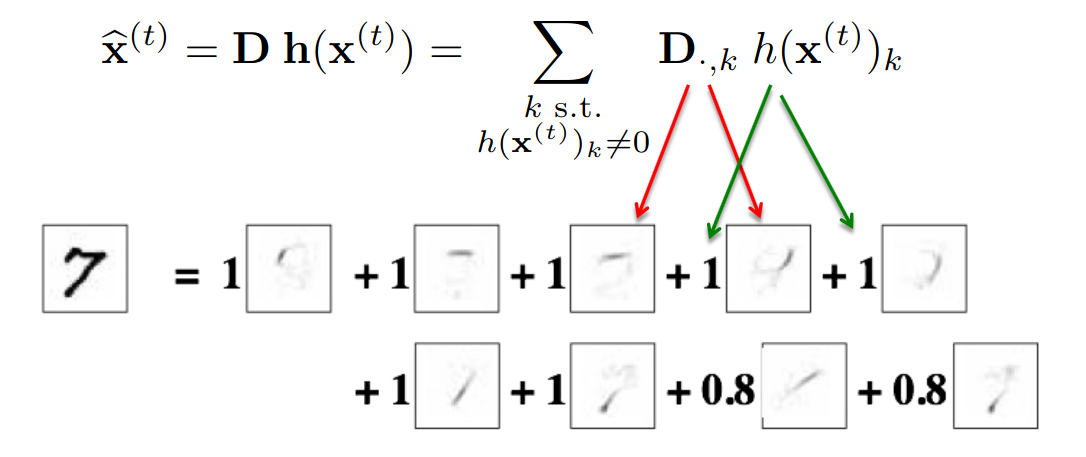
\includegraphics[scale=0.4]{img/sparse_coding.png}
    \end{center}
    Let's think about how we can optimize the objective function w.r.t. $\mathbf{h}$, keeping $\mathbf{D}$ constant. We can do stochastic gradient descent, which gives us the steps
    \[\nabla_{\mathbf{h}^{(t)}} \mathcal{L}(\mathbf{x}^{(t)}) = \mathbf{D}^T (\mathbf{D} \mathbf{h}^{(t)} - \mathbf{x}^{(t)}) + \lambda \, \mathrm{sign}(\mathbf{h}^{(t)})\]
    but this wouldn't achieve sparsity since it overshoots the $0$ all the time. Therefore, we can clip it, or we can use proximal gradient descent/ISTA to take a step, and shrink the parameters according to the L1 norm. 
    \begin{align*} 
        \mathbf{h}^{(t)} & = \mathbf{h}^{(t)} - \alpha \mathbf{D}^T (\mathbf{D} \mathbf{h}^{(t)} - \mathbf{x}^{(t)}) \\
        \mathbf{h}^{(t)} & = \mathrm{shrink}(\mathbf{h}^{(t)}, \alpha \lambda)
    \end{align*}
        where $\mathrm{shrink}(\mathbf{a}, \mathbf{b}) = [\ldots, \mathrm{sign}(a_i)\, \max(|a_i| - b_i, 0), \ldots]$. This is guaranteed to converge if $1/\alpha$ is bigger than the largest eigenvalue of $\mathbf{D^T} \mathbf{D}$.  
    

  \subsection{Independent Component Analysis} 

    Another special case of linear factor model is ICA. In our setting, let us just assume that $\mathbf{b} = \mathbf{0}$ and $\epsilon = 0$. That is, we have the simple model 
    \[\mathbf{x} = \mathbf{W} \mathbf{h}\] 
    In here, $\mathbf{x} \in \mathbb{R}^d$ is a mixture vector and $\mathbf{W} \in \mathbb{R}^{d \times d}$ is a \textbf{mixing matrix}. Note that the hidden $\mathbf{h}$ has the same dimensions as $\mathbf{x}$, but this can be generalized to rectangular matrices. Both $\mathbf{W}$ and $\mathbf{h}$ are unknown, and we need to recover them given $\mathbf{x}$. In \textbf{linear ICA}, we have two strong assumptions: 
    \begin{enumerate} 
        \item Each component of $\mathbf{h}$ is independent (not just uncorrelated). This is an easy enough assumption to intuit.  
        \item Independent components of $\mathbf{h}$ must \textit{not} be Gaussian. This is needed for us to be able to ``unmix" the signals. To see why, just suppose $\mathbf{h}$ was Gaussian, and so the vector $\mathbf{R} \mathbf{h}$ is also Gaussian for any invertible $\mathbf{R}$. Therefore, we could find an infinite number of solutions of form 
        \[\mathbf{x} = \mathbf{W} \mathbf{R}^{-1} \mathbf{R} \mathbf{h}\]
        and I have no way to separate them. 
    \end{enumerate}

    There are further ambiguities with ICA. 
    \begin{enumerate}
        \item Estimating the latent components up to a scaling factor. 
            \[\mathbf{x} = (\alpha \mathbf{W}) (\frac{1}{\alpha} \mathbf{h}) \text{ for some } \alpha > 0\]
            We can fix this by forcing $\mathbb{E}[h_i^2] = 1$. However, there is still an ambiguity for the sign of hidden components, but this is insignificant in most applications. 

        \item Estimating the components up to permutation. We have 
            \[\mathbf{x} = \mathbf{W} \mathbf{P}^{-1} \mathbf{P} \mathbf{h}\] 
            for some permutation matrix $\mathbf{P}$. 
    \end{enumerate}

    Now let's see how linear ICA actually estimates $\mathbf{W}$ and $\mathbf{h}$. Once $\mathbf{W}$ is estimated, the latent components of a given test mixture vector, $\mathbf{x}^\ast$ is computed by $\mathbf{h}^\ast = \mathbf{W}^{-1} \mathbf{x}^\ast$. So now all there's left to do is to estimate $\mathbf{W}$, which we want to estimate so that $\mathbf{W}^{-1} \mathbf{x}$ is far from Gaussian. The reason for this is that given a bunch of independent non-Gaussian $h_i$'s, if we mix them with a matrix that is not $\pm \mathbf{I}$ , then by CLT, a linear combination of random variables will tend to be Gaussian, and so for an arbitrary $\mathbf{W}$ we would expect $\mathbf{x}$ to be Gaussian. Therefore, what we want to do is guess some matrix $\mathbf{A}$, and compute 
    \[\mathbf{A} \mathbf{x} = \mathbf{A} \mathbf{W} \mathbf{h}\]
    and if we get things right, $\mathbf{A} \approx \mathbf{W}^{-1}$, and the result of $\mathbf{A} \mathbf{x}$ would look pretty non-Gaussian. If it it not the case, then $\mathbf{A W}$ will still be some mixing matrix, and so $\mathbf{A} \mathbf{x}$ would look Gaussian. So now the question reduces to how do we choose this $\mathbf{A}$? There are multiple ways to measure non-Gaussianity: 
    \begin{enumerate} 
        \item The absolute or squared kurtosis, which is $0$ for Gaussians. This is a differentiable function w.r.t. $\mathbf{W}$, so we can try maximizing it. This is done for the sample kurtosis, of course.  
        \item Another measure is by maximizing the neg-entropy. 
    \end{enumerate}

    We can perform this on three mixed signals with additive noise, and ICA does very well, though again some recovered signals are scaled or permuted weirdly. 
    \begin{center}
      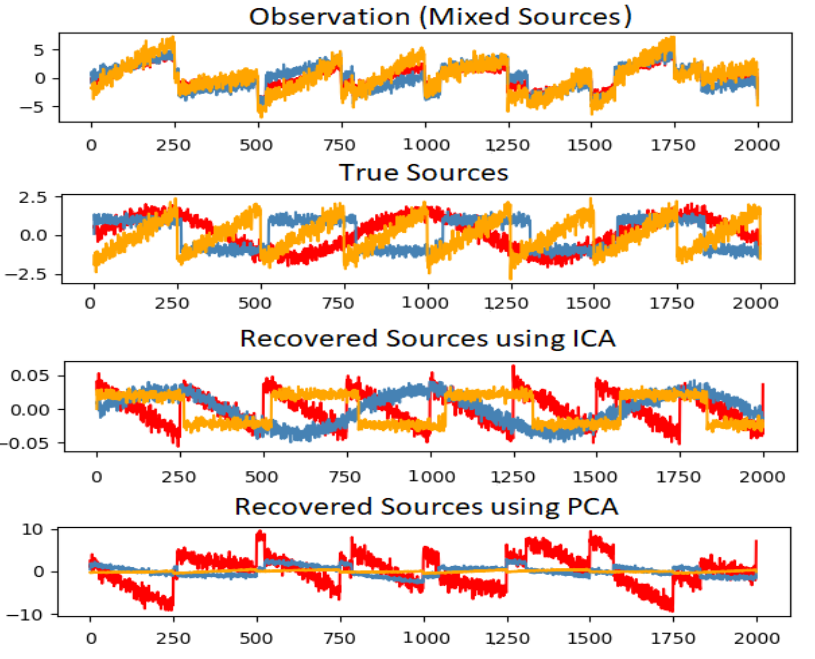
\includegraphics[scale=0.4]{img/ICA_example.png}
    \end{center}

  \subsection{Slow Feature Analysis}

    Slow feature analysis also another special case of a linear factor model that uses information from time signals to learn invariant features. It is motivated by a general principle called the \textbf{slowness principle}. The idea is that the important characteristics of scenes change very slowly compared to the individual measurements that make up a description of a scene. For example, in computer vision, individual pixels can change very rapidly. If a zebra moves from left to right across the image, an individual pixel wil rapidly change from black to white. By comparison, the feature indicating whether a zebra is in the image will not change at all, and the feature describing the zebra's position will change slowly. Therefore, we want to regularize our model to learn features that change slowly over time.  

    We can apply the slowness principle to any differentiable model trained with gradient descent. That is, we can add the following term to the loss function: 
    \[\lambda \sum_i d\big( f(\mathbf{x}^{(t+1)}), f(\mathbf{x}^{(t)}) \big)\]
    where $\lambda$ is a hyperparameter determining the strength of the slowness regularization term, $t$ is the time index, $f$ is the feature extractor to be regularized, and $d$ is the distance between $f(\mathbf{x}^{(t)})$ and $f(\mathbf{x}^{(t+1)})$. A common choice for $d$ is the mean squared difference. 

    Essentially, given a set of time-varying input signals $\mathbf{x}^{(t)}$, SFA learns a nonlinear function $f$ that transforms $\mathbf{x}$ into slowly-varying output signals $\mathbf{y}$. Obviously, we can't just take some trivial function like $f = 0$, so we have the following constraints 
    \begin{align*}
        \mathbb{E}_t [ f(\mathbf{x}^{(t)})_i]  & = 0 \\ 
        \mathbb{E}_t [ f(\mathbf{x}^{(t)})_i^2] & = 1 
    \end{align*}
    \begin{center} 
        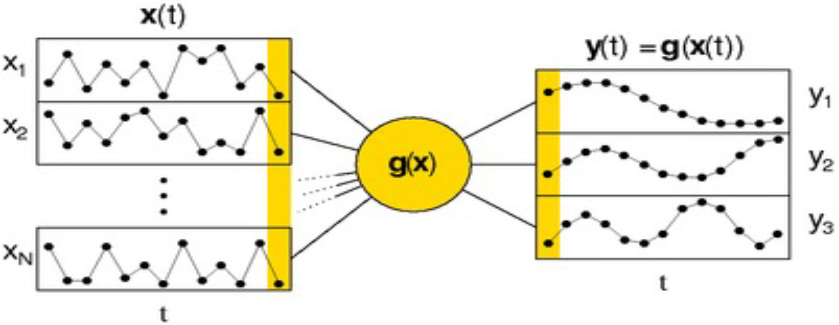
\includegraphics[scale=0.4]{img/slow_feature.png}
    \end{center}
    We can restrict the nonlinear $f$ to some subspace of functions, and this becomes a standard optimization problem where we solve 
    \[\min_\theta \mathbb{E}_t \big[ \big( f(\mathbf{x}^{(t+1)})_i - f(\mathbf{x}^{(t)})_i \big)^2 \big]\]


  \subsection{Latent Dirichlet Allocation} 

  \subsection{UMAP}

  \subsection{t-SNE}

\section{Practical Methods} 

  \subsection{Model Selection} 

    We've talked about the theory and implementation behind all these models, but in practice, how do we even use them? If we are trying to predict lung cancer in a patient, do we use linear regression, a nonparametric model, or something else? It's not clear at all what to do with the data. Unfortunately, this just comes with domain expertise and experience with data, but we can provide some general pointers. 

    As stated before, we have the flexibility to choose whatever model to train on. So how do we choose which form is the best? Well this is just an assumption that most researchers make, and this is called \textbf{model selection}. 

    \begin{example}[Polynomial Regression]
      The number of terms $M$, i.e. the degree $M-1$ of the polynomial 
        \[h_{\boldsymbol{\theta}} (x) = w_0 + w_1 x + w_2 x^2 + \ldots + w_{M-1} x^{M-1}\]
      in polynomial regression gives us models with different complexities, where $\mathcal{M}_M$ determines the model with a $M-1$th degree polynomial. 
    \end{example}

    \begin{example}
      Suppose I have data sampled data $x^{(1)}, \ldots, x^{(N)}$ on age at death for $N$ people from an unknown distribution $X$. Then, possible models that model the distribution are 

      \begin{enumerate}
        \item $\mathcal{M}_1$: the exponential distribution $p(x \mid \lambda) = \lambda e^{-\lambda y}$ with parameter $\theta = \lambda$. 
        \item $\mathcal{M}_2$: the gamma distribution $p(y \mid a, b) = (b^a / \Gamma(a)) y^{a - 1} e^{- by}$ with parameter $\boldsymbol{\theta} = (a, b)$. 
        \item $\mathcal{M}_3$: the log-normal distribution with $X \sim N (\mu, \sigma^2)$ where ${\boldsymbol{\theta}} = (\mu, \sigma^2)$. 
      \end{enumerate}
    \end{example}

    \begin{example}
      A mixture of Gaussians model 
        \[p(\mathbf{y}) = \sum_{m=1}^M \pi_m N(\mathbf{y} \mid \boldsymbol{\mu}_m, \boldsymbol{\Sigma}_m )\]
      has submodels where we must determine the number of Gaussians $M$. 
    \end{example}

    Now if we assume that the actual true distribution $X$ or the true regressor $\mathbb{E}[Y\mid X]$ is contained within our model $\mathcal{M}$, then we say our model is \textbf{well-specified}. But since researchers have no idea what the data generating process is, so $\mathbb{E}[Y\mid X] \not\in \mathcal{M}$. Hence there is the saying that saying that ``all models are wrong," since we never know what the true data generating process is, and thus the quantity 

      \[\mathbb{E}[Y \mid X] - h_{\boldsymbol{\theta}}^\ast (X)\]

    where $h_{\boldsymbol{\theta}}^\ast (X)$ is the optimized hypothesis functions within $\mathcal{M}$, will always be nonzero. How close we can get this quantity to $0$ determines how useful the model is, and a misspecified model is fundamentally a convenient (or even necessary) assumption on the distribution underlying the data, which may only be a reasonable approximation. 

  \subsection{Feature Engineering} 

    This is also very domain specific. 

  \subsection{Data Preprocessing}

    \subsubsection{Feature Extraction}

      The simplest linear function for regression is simply 
      \[h_\mathbf{w} (\mathbf{x}) = w_0 + w_1 x_1 + \ldots + w_D x_D\]
      This is called linear regression not because $h$ is a linear function of $\mathbf{x}$. It is a linear function of $\mathbf{w}$. Therefore, we can fix nonlinear functions $\phi_j (\mathbf{x})$ and consider linear combinations of them. 

        \[h_\mathbf{w} (\mathbf{x}) = w_0 + \sum_{j=1}^{M-1} w_j \phi_j (\mathbf{x})\]

      We usually choose a dummy basis function $\phi_0 (\mathbf{x}) = 1$ for notational convenience, so that if $\boldsymbol{\phi}$ is the vector of the function $\phi_j$, then we can write $h_\mathbf{w} (\mathbf{x}) = \mathbf{w}^T \boldsymbol{\phi} (\mathbf{x})$. This mapping from the original variables $\mathbf{x} \in \mathbb{R}^D$ to the basis functions $\{\phi_j (\mathbf{x})\}$, which span a linear function space of dimension $M$, is called \textbf{preprocessing} or \textbf{feature extraction} of the data. 

      \begin{example}
        Here are some examples of how we can extract features. 
        \begin{enumerate}
          \item The mapping from a single variable $x$ to its powers 
            \begin{equation}
              x \mapsto (1, x, x^2, \ldots, x^{M-1})
            \end{equation}
          \item The mapping from a configuration of $K$ atoms with their momenta in $\mathbb{R}^{6K}$ to their atomic cluster expansion polynomials. 
          \item The Legendre polynomials, which form an orthonormal basis in the space of polynomials. 
          \item Using equally spaced Gaussian basis functions over the dataset. 
            \begin{figure}[H]
              \centering
              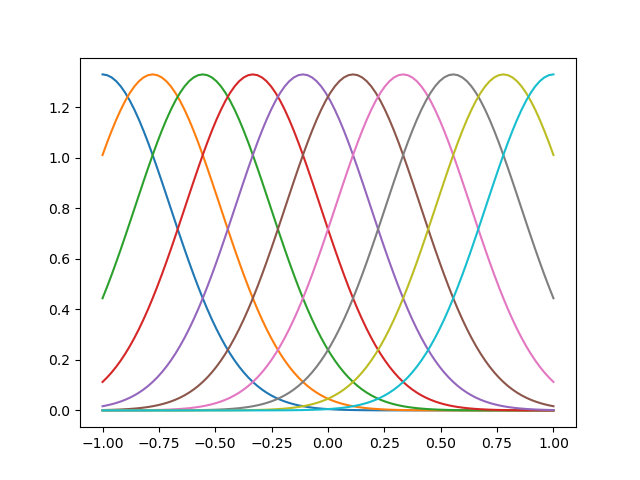
\includegraphics[scale=0.5]{img/Gaussian_basis_functions.png}
              \caption{Gaussian basis functions over the interval $[-1, 1]$ with standard deviation of $0.3$}
              \label{fig:Gaussian_basis_functions}
            \end{figure}
        \end{enumerate}
      \end{example}

      Changing the input space from $D$ dimensions to $M$ dimensions (i.e. extracting our $M$ features) gives the design matrix 
      \begin{equation}
        \mathbf{X} = \begin{pmatrix} 
          \mathbf{x}^{(1)} \\ \mathbf{x}^{(2)} \\ \mathbf{x}^{(3)} \\ \vdots \\ \mathbf{x}^{(n)} \end{pmatrix} \implies \boldsymbol{\Phi} = \begin{pmatrix}
        \text{---} & \phi(\mathbf{x}^{(1)}) & \text{---} \\
        \text{---} & \phi(\mathbf{x}^{(2)}) & \text{---} \\
        \vdots & \vdots & \vdots \\
        \text{---} & \phi(\mathbf{x}^{(n)}) & \text{---}
        \end{pmatrix}
      \end{equation}


      We have shown that the $\texttt{PolynomialFeatures}$ transformer converts our features to a polynomial basis. We can do this for an arbitrary number of features, for example if we map $D = 2$ to a second degree polynomial, we would have the transformation 

      \[(x_1, x_2) \mapsto (1, x_1, x_2, x_1^2, x_1 x_2, x_2^2)\]

      \begin{lstlisting}
      >>> import numpy as np
      >>> from sklearn.preprocessing import PolynomialFeatures
      >>> X = np.arange(6).reshape(3, 2)
      >>> X
      array([[0, 1],
             [2, 3],
             [4, 5]])
      >>> poly = PolynomialFeatures(2)
      >>> poly.fit_transform(X)
      array([[ 1.,  0.,  1.,  0.,  0.,  1.],
             [ 1.,  2.,  3.,  4.,  6.,  9.],
             [ 1.,  4.,  5., 16., 20., 25.]])
      \end{lstlisting}
      Sometimes, we are only worried about the interaction terms among features, so we can set the parameter \texttt{interaction\_only=True}, which would, in the third degree case, transform the features 

        \[(x_1, x_2, x_3) \mapsto (1, x_1, x_2, x_3, x_1 x_2, x_1 x_3, x_2 x_3, x_1 x_2 x_3)\]

      \textbf{Spline transformers} are piecewise polynomials, which is also built in. We notice that it is cumbersome to transform the dataset \texttt{X} with the transformer, store it into another variable, and train the model on that. We can ``combine" the transforming (even multiple layers of transformers) and the model by implementing a ``pipeline," which is initialized by inputting a list of tuples (name and the object) and has the same methods as the model. 

      \begin{lstlisting}
      from sklearn.pipeline import Pipeline
      model = Pipeline([("poly_transform", PolynomialFeatures(degree=2)), 
                        ("lin_regression", LinearRegression())
                        ]) 
      model.fit(X, y)
      \end{lstlisting}

      Now, let's talk about how we can implement a custom transformer. We basically have to create a new subclass that implements the \texttt{fit} (which always returns \texttt{self}) and the \texttt{transform} (which returns the transformed matrix) methods. Here we show for Gaussian basis functions. 

      \begin{lstlisting}
      from sklearn.base import BaseEstimator, TransformerMixin

      class GaussianFeatures(BaseEstimator, TransformerMixin):
          """Uniformly spaced Gaussian features for one-dimensional input"""
          
          def __init__(self, N, width_factor=2.0):
              self.N = N
              self.width_factor = width_factor
              
          def fit(self, X, y=None):
              # create N centers spread along the data range
              self.centers_ = np.linspace(X.min(), X.max(), self.N)
              self.width_ = self.width_factor * (self.centers_[1] - self.centers_[0])
              return self
              
          def transform(self, X): 
              transformed_rows = []
              for mu in self.centers_: 
                  transformed_rows.append(stats.norm.pdf(X, mu, self.width_))
              
              return np.hstack(tuple(transformed_rows))

      model = Pipeline([("gauss_transform", GaussianFeatures(20)), 
                        ("lin_regression", LinearRegression())
                        ]) 

      N = 60
      X = np.random.uniform(-1, 1, size=(N, 1)) 
      Y = true_func(X) + np.random.normal(0, 0.3, size=(N, 1)) 

      model = Pipeline([("gauss_transform", GaussianFeatures(10)), 
                    ("lin_regression", LinearRegression())
                    ]) 
      model.fit(X, Y)
      \end{lstlisting} 

      If we would like to impelment the fourier expansion of a function of form 

        \[f(x) = \frac{1}{2} a_0 + \sum_{n=1}^N a_n \cos(n x) + \sum_{n=1}^N b_n \sin(n x)\]

      Then we would create the basis functions according to 

      \begin{lstlisting}
      class FourierFeatures(BaseEstimator, TransformerMixin): 
          "Fourier Expansion for one-dimensional input"
          
          def __init__(self, N): 
              self.N = N 
              
          def fit(self, X, Y=None): 
              return self
          
          def transform(self, X): 
              transformed_columns = [] 
              transformed_columns.append(np.ones(shape=X.shape))
              
              for n in range(self.N): 
                  transformed_columns.append(np.sin(n * X))
                  transformed_columns.append(np.cos(n * X))
                  
              print(np.hstack(tuple(transformed_columns)).shape)
              return np.hstack(tuple(transformed_columns))
      \end{lstlisting} 
      and both of them would give the following fits to our original function $f(x) = \sin(2\pi x) + 2 \cos(x - 1.5)$. 
      \begin{figure}[H]
          \centering
          \begin{subfigure}[b]{0.48\textwidth}
          \centering
              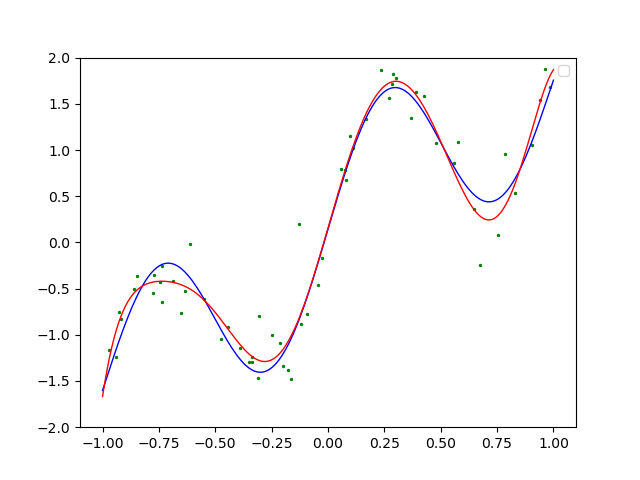
\includegraphics[width=\textwidth]{img/Gaussian_Fit.png}
              \caption{Fitting with 10 Gaussian basis functions. }
              \label{fig:gaussian_basis}
          \end{subfigure}
          \hfill 
          \begin{subfigure}[b]{0.48\textwidth}
          \centering
              \includegraphics[width=\textwidth]{img/Fourier_Fit.png}
              \caption{Fitting with 10 Fourier basis functions. }
              \label{fig:fourier_basis}
          \end{subfigure}
          \caption{}
          \label{Coincide_mean}
      \end{figure}

    \subsubsection{Standardizing Data}

      \textbf{Standardizing} typically meanss that our featuers will be rescaled to have the properties of a standard normal distribution with mean of $0$ and a standard deviation of $1$. Here are a few methods to scale our data, with their results shown on a dataset of $30$ points in $\mathbb{R}^2$. 
      \begin{enumerate}
          \item \textbf{StandardScaler}: This is probably the most used method for standardizing data. It standardizes features by removing the mean and scaling to unit variance. The standard score of a sample $x^{(n)}$ is $(x - \bar{x})/S$ where $\bar{x}$ is the mean of the training samples and $S$ is the standard deviation of the training samples. 
          \begin{lstlisting}
          from sklearn.preprocessing import StandardScaler
          scaler = StandardScaler()
          scaled_data = scaler.fit_transform(data)
          \end{lstlisting}

          \item \textbf{MinMaxScaler}: While not technically "standardization," MinMaxScaler is another preprocessing method for scaling. It transforms features by scaling each feature to a given range, typically between zero and one, or so that the maximum absolute value of each feature is scaled to unit size. 
          \begin{lstlisting}
          from sklearn.preprocessing import MinMaxScaler
          scaler = MinMaxScaler()
          scaled_data = scaler.fit_transform(data)
          \end{lstlisting}

          \item \textbf{MaxAbsScaler}: This scaler works similarly to the MinMaxScaler but scales in a way that the training data lies within the range $[-1, 1]$ by dividing through the largest maximum value in absolute value. It is meant for data that is already centered at zero or sparse data. 
          \begin{lstlisting}
          from sklearn.preprocessing import MaxAbsScaler
          scaler = MaxAbsScaler()
          scaled_data = scaler.fit_transform(data)
          \end{lstlisting}

          \item \textbf{RobustScaler}: This scaler removes the median and scales the data according to the quantile range (defaults to IQR: Interquartile Range). It's robust to outliers, which makes it a good choice if you have data with possible outliers. 
          \begin{lstlisting}
          from sklearn.preprocessing import RobustScaler
          scaler = RobustScaler()
          scaled_data = scaler.fit_transform(data)
          \end{lstlisting} 

          \item \textbf{QuantileTransformer}: Note that the presence of outliers messes with our scaling. More generally for skewed distributions (like an exponential), a linear transformation does not take care of these outliers, so we would like some nonlinear preprocessing algorithm. One common one is the QuantileTransformer, which takes the quantiles (percentiles) of the dataset and transforms then so that those are equidistant from each other. By default, it divides up the data into 1000 quantiles. 
          \begin{lstlisting}
          from sklearn.preprocessing import QuantileTransformer
          transformer = QuantileTransformer(n_quantiles = 100, output_distribution='normal')
          transformed_data = transformer.fit_transform(data)
          \end{lstlisting}
      \end{enumerate}

      Let's talk about how these scalers will work on some data. We take a wine data with the two variables representing fixed acidity and volatile acidity. 
        \begin{figure}[H]
          \centering
          \begin{subfigure}[b]{0.32\textwidth}
          \centering
              \includegraphics[width=\textwidth]{img/Standard_scaler1.png}
              \caption{Original Data}
              \label{fig:no_scaling}
          \end{subfigure}
          \hfill
          \begin{subfigure}[b]{0.32\textwidth}
          \centering
              \includegraphics[width=\textwidth]{img/Standard_scaler2.png}
              \caption{StandardScaler}
              \label{fig:standard_scaler}
          \end{subfigure}
          \hfill
          \begin{subfigure}[b]{0.32\textwidth}
          \centering
              \includegraphics[width=\textwidth]{img/MinMax_Scaler.png}
              \caption{MinMaxScaler}
              \label{fig:minmax_scaler}
          \end{subfigure}

          \begin{subfigure}[b]{0.32\textwidth}
          \centering
              \includegraphics[width=\textwidth]{img/MaxAbs_Scaler.png}
              \caption{MaxAbsScaler}
              \label{fig:maxabs_scaler}
          \end{subfigure}
          \hfill
          \begin{subfigure}[b]{0.32\textwidth}
          \centering
              \includegraphics[width=\textwidth]{img/Robust_Scaler.png}
              \caption{RobustScaler}
              \label{fig:robust_scaler}
          \end{subfigure}
          \hfill
          \begin{subfigure}[b]{0.32\textwidth}
          \centering
              \includegraphics[width=\textwidth]{img/Quantile_Scaler.png}
              \caption{QuantileTransformer}
              \label{fig:quantile_transformer}
          \end{subfigure}
          
          \caption{The StandardScaler simply standardizes the data to have $0$ mean and unit variance.}
          \label{Scalers}
        \end{figure}

      It's important to note that whether you should standardize your data and how you should do it depends on the specific characteristics of your data and the machine learning algorithm you're using. For example, some algorithms, like many in deep learning, assume that all features are on the same scale. Others, like Decision Trees and Random Forests, do not require feature scaling at all. 

  \subsection{Data Augmentation}

\section{Archive}

  \subsection{Bayesian Probability}

    Now this book puts a heavy emphasis on Bayesian probabilistic models. For now, we will denote $p(X)$ to be the distribution of a random variable $X$. We capture our assumptions about the model parameter $\mathbf{w}$ with a prior distribution $p(\mathbf{w})$. Our likelihood $p(\mathcal{D} \mid \mathbf{w})$ is the conditional distribution of getting the data $\mathcal{D}$ from our model with parameter $\mathbf{w}$. Therefore, Bayes theorem is expressed 
    \[p(\mathbf{w} \mid \mathcal{D}) = \frac{p(\mathcal{D} \mid \mathbf{w}) \, p(\mathbf{w})}{p(\mathcal{D})}\]
    The denominator $p(\mathcal{D})$ is a normalizing term equal to $\int p(\mathcal{D} \mid \mathbf{w}) \, p(\mathbf{w}) \,d\mathbf{w}$, and for high dimensional $\mathcal{W}$ it may not be feasible to compute this integral without monte carlo sampling. Therefore, we focus on the numerator terms and remember the rule 
    \[\text{posterior} \propto \text{likelihood} \times \text{prior}\]

    For clarification, $\mathcal{D}$ can represent different things depending on the problem: 
    \begin{enumerate}
        \item In a density estimation problem, where we have a single dataset $\mathbf{X}$, $\mathcal{D} = \mathbf{X}$ since this data tells us information about which distribution it could come from. 
        \item In a regression problem, $\mathcal{D} = \mathbf{Y}$, that is, $\mathcal{D}$ will always be the output data, not the input data $\mathbf{X}$. We can think of the input data $\mathbf{X}$ as always being fixed, and it is upon observation of the \textit{outputs} $\mathbf{Y}$ on these inputs that gives us information. 
    \end{enumerate}

    In both the frequentist and Bayesian settings, the likelihood $p(\mathcal{D} \mid \mathbf{w})$ plays a central role. In the frequentist setting, the process is divided into two steps: 
    \begin{enumerate}
        \item We optimize $\mathbf{w}$ with some \textbf{estimator}, with a popular one being the \textbf{maximum likelihood estimator}. A popular estimator is \textbf{maximum likelihood}, which seeks to maximize $p(\mathcal{D} \mid \mathbf{w})$ w.r.t. $\mathbf{w}$. 
        \item We optimize $\mathbf{w}$ with some \textbf{estimator}, with a popular one being the \textbf{maximum likelihood estimator}. A popular estimator is \textbf{maximum likelihood}, which seeks to maximize $p(\mathcal{D} \mid \mathbf{w})$ w.r.t. $\mathbf{w}$. 
        \item We fix the optimized $\mathbf{w}^\ast$ and error bars on this estimate are obtained by considering the distribution of possible datasets $\mathcal{D}$. One approach is \textbf{bootstrapping}, which goes as follows. Given our original dataset $\mathbf{X} = \{x^{(1)}, \ldots, x^{(N)}\}$, we can create a new dataset $\mathbf{X}^\prime$ by sampling $N$ points at random from $\mathbf{X}$, with replacement, so that some points in $\mathbf{X}$ may be replicated in $\mathbf{X}^\prime$, whereas other points in $\mathbf{X}$ may be absent in $\mathbf{X}^\prime$. This process is repeated $L$ times to generate $L$ different datasets. Then, we can look at the variability of prediction between the different bootstrap data sets. 
    \end{enumerate}
    In a Bayesian setting, there is only a single dataset $\mathcal{D}$ and the uncertainity in the parameters is expressed through a probability distribution over $\mathbf{w}$. It also includes prior knowledge naturally in the form of prior distributions. 

  \subsection{Density Estimation}

    \subsubsection{Frequentist Approach}

      As a start, let us have a dataset of observations $\mathbf{X} = \{x^{(1)}, \ldots, x^{(n)}\}$ assuming that they are all iid from $X \sim N(0, 1)$ distribution. Since this is iid, we can look at the joint distribution $X^N$ on $\mathbb{R}^N$ and get the likelihood of form
      \[p(\mathbf{X} \mid \mu, \sigma^2) = \prod_{n=1}^N p_X (x^{(n)} \mid \mu, \sigma^2)\]
      which in turn gives the log-likelihood as 
      \[\ln p(\mathbf{X} \mid \mu, \sigma^2) = -\frac{1}{2 \sigma^2} \sum_{n=1}^N (x_n - \mu)^2 - \frac{N}{2} \ln \sigma^2 - \frac{N}{2} \ln(2 \pi)\]
      This is a function of two variables, $\mu$ and $\sigma^2$ and we can optimize it to get the maximum likelihood estimates of 
      \[\mu_{ML} = \frac{1}{N} \sum_{n=1}^N x_n \text{ and } \sigma^2_{ML} = \frac{1}{N} \sum_{n=1}^N (x_n - \mu_{ML})^2\]
      However, as we saw in the previous section, the estimate for $\sigma^2$ is biased by a factor of $(N-1)/N$, and this is an intrinsic flaw in the frequentist approach. 

    \subsubsection{Bayesian Approach}

      In the Bayesian approach, we want to model
      \[p(x \mid \mathcal{D}) = \int p(x \mid \mathbf{w}) \, p(\mathbf{w} \mid \mathcal{D}) \; d\mathbf{w}\]

  \subsection{Regression with Regularization}

    \subsubsection{Frequentist's Maximum Likelihood Approach}

      Now given the hypothesis function $h_\mathbf{w}$, researchers assume that the relationship between the $X$ and $Y$ values are captured by 
      \[Y = h_\mathbf{w}(X) + \epsilon\]
      where $\epsilon$ is some residual noise, also a random variable. Researchers assume that this random variable has a nice form. One popular choice is that $\epsilon \sim N(0, \sigma^2)$ since if we assume that this error is due to a large number of weakly dependent unknown factors, then by CLT we can assume that their sum is Gaussian. But ultimately this is just another assumption. With this Gaussian assumption, we can assume that each input output pair $(x^{(n)}, y^{(n)})$ is generated by form $y^{(n)} = h_\mathbf{w} (x^{(n)}) + \epsilon$ and so the conditional distribution of $y^{(n)}$ given $X^{(n)}$ is 
      \[Y \mid X = x^{(n)} \sim N( h_\mathbf{w} (x^{(n)}), \sigma^2) \]
      and therefore, the probability of getting $y^{(n)}$ given $x^{(n)}$ is modeled by the conditional pdf 
      \[p_{Y \mid X = x^{(n)}} (y^{(n)}) = \frac{1}{\sqrt{2 \pi \sigma^2}} \exp \bigg( -\frac{[ y^{(n)} - h_\mathbf{w} (x^{(n)}) ]^2}{2 \sigma^2} \bigg)\]
      Extending this to the dataset $\mathcal{D} = \mathbf{Y}$ coming from the $N$-fold joint distribution of $X$, by independence this distribution is a multivariate Gaussian
      \[Y^n \mid X^n = \mathbf{X} \sim N( h_\mathbf{w} (\mathbf{X}), \sigma^2 \mathbf{I})\]
      where by abuse of notation, $h_\mathbf{w} (\mathbf{X})$ is $h_\mathbf{w}$ operated element-wise on the vector $\mathbf{X}$, and $\mathbf{I}$ is the $N \times N$ identity matrix. The pdf is 
      \begin{align*}
          p_{Y^n \mid X^n = \mathbf{X}} (\mathbf{Y}) & = \prod_{n=1}^N p_{Y \mid X = x^{(n)}} (y^{(n)}) \\
          & = \prod_{n=1}^N \frac{1}{\sqrt{2 \pi \sigma^2}} \exp \bigg( -\frac{[ y^{(n)} - h_\mathbf{w} (x^{(n)}) ]^2}{2 \sigma^2} \bigg)
      \end{align*}
      The two parameters of interest here that we would like to maximize are $\mathbf{w}$ and $\sigma^2$. We can take the log of this function to maximize this, which gives us 
      \[\ell(\mathbf{w}, \sigma^2) = -\frac{1}{\sigma^2} E_D (\mathbf{w}) - \frac{N}{2} \ln \sigma^2 - \frac{N}{2} \ln(2\pi)\]
      and here we can see that maximizing the likelihood w.r.t. $\mathbf{w}$ is equal to minimizing the sum-of-squares error function $E_D(\mathbf{w}) = -\frac{1}{2} \sum_{n=1}^N [ y^{(n)} - h_\mathbf{w} (x^{(n)})]^2 $. Therefore, a maximum likelihood estimation under a Gaussian residual assumption implies minimization of the sum-of-squares error function! To maximize with respect to both $\mathbf{w}$ and $\sigma^2$, we can use the fact that this function is $C^1$ (continuously differentiable), and so we just need to find where the partials are $0$. Ultimately, we can just optimize for $\mathbf{w}$ first and then solve for $\sigma^2$. If $h_\mathbf{w}$ was linear (not necessarily in $\mathbf{x}$, but with $\mathbf{w}$), then we can transform the $x_d$ values, get the proper design matrix $\boldsymbol{\Phi}$, and compute 
      \[\mathbf{w}_{ML} = (\boldsymbol{\Phi}^T \boldsymbol{\Phi})^{-1} \boldsymbol{\Phi}^T \mathbf{Y}\]
      If we add a ridge penalty term to get $E(\mathbf{w}) = E_D (\mathbf{w}) + \frac{\lambda}{2} ||\mathbf{w}||^2_2$, then this results in solving the matrix equation
      \[\mathbf{w}_{ML} = (\boldsymbol{\Phi}^T \boldsymbol{\Phi} + \lambda \mathbf{I})^{-1} \boldsymbol{\Phi}^T \mathbf{Y}\]
      With these optimized parameters, we have a \textbf{probabilistic model} in which given a new value $\hat{\mathbf{x}}$, we can predict the conditional distribution of $\hat{y}$ to be 
      \[p(y^\prime \mid \hat{\mathbf{x}}, \mathbf{w}_{ML}, \sigma^2_{ML}) = N(\hat{y} \mid h_{\mathbf{W}_{ML}} (\mathbf{x}^\prime), \sigma^2_{ML})\]

      % Now, even if we choose precisely $g(X) = \mathbb{E}[Y \mid X]$, this will in most cases not be a perfect indicator of $Y$ since usually $\sigma(Y) \not\subset \sigma(X)$. Therefore, there is a \textbf{residual term} $\epsilon$ that is precisely the difference between $g(X)$ and $Y$. 
      % \[Y = g(X) + \epsilon\]
      % We do not know what this $\epsilon$ even is besides the fact that it does not live in the space of all $\sigma(X)$-measurable functions (since if it did, then it would be captured by $g$). We also know from the tower property that 
      % \[\mathbb{E}[\epsilon] = \mathbb{E}[Y - \mathbb{E}[Y \mid X]] = \mathbb{E}[Y] - \mathbb{E}[Y] = 0\]

    \subsubsection{Bayesian Approach}

      We will now demonstrate how having a normal $\alpha \mathbf{I}$ prior around the origin in a Bayesian setting is equivalent to having a ridge penalty of $\lambda = \sigma^2 / \alpha^2$ in a frequentist setting. If we have a Gaussian prior of form 
      \[p(\mathbf{w} \mid \alpha^2) = N(\mathbf{w} \mid \mathbf{0}, \alpha^2 \mathbf{I}) = \bigg( \frac{1}{2 \pi \alpha^2} \bigg)^{M/2} \exp \bigg( -\frac{1}{2\alpha^2} ||\mathbf{w}||^2_2 \bigg)\]
      We can use Bayes rule to compute 
      \begin{align*}
          p(\mathbf{w} \mid \mathbf{X}, \mathbf{Y}, \alpha^2, \sigma^2) & \propto p(\mathbf{Y} \mid \mathbf{w}, \mathbf{X}, \alpha^2, \sigma^2) \, p(\mathbf{w} \mid \mathbf{X}, \alpha^2, \sigma^2) \\
          & = \bigg[ \prod_{n=1}^N p(y^{(n)} \mid \mathbf{w}, \mathbf{x}^{(n)}, \alpha^2, \sigma^2 )\bigg] \, p(\mathbf{w} \mid \mathbf{X}, \alpha^2, \sigma^2) \\
          & = \bigg[ \prod_{n=1}^N \frac{1}{\sqrt{2 \pi \sigma^2}} \exp \bigg( - \frac{(y^{(n)} - h_\mathbf{w} (x^{(n)}))^2}{2 \sigma^2} \bigg) \bigg] \cdot \bigg( \frac{1}{2 \pi \alpha^2} \bigg)^{M/2} \exp \bigg( -\frac{1}{2\alpha^2} ||\mathbf{w}||^2_2 \bigg)
      \end{align*}
      and taking the negative logarithm gives us 
      \[\ell(\mathbf{w}) = \frac{1}{2\sigma^2} \sum_{n=1}^N \big(y^{(n)} - h_\mathbf{w} (\mathbf{x}^{(n)}) \big)^2 + \frac{N}{2}\ln{\sigma^2} + \frac{N}{2} \ln(2\pi) - \frac{M}{2} \ln(2\pi \alpha^2) + \frac{1}{2 \alpha^2} ||\mathbf{w}||_2^2\]
      taking out the constant terms relative to $\mathbf{w}$ and multiplying by $2 \sigma^2$ (which doesn't affect optima) gives us the ridge penalized error with a penalty term of $\lambda = \sigma^2 / \alpha^2$. 
      \[E(\mathbf{w}) = \frac{1}{2} \sum_{n=1}^N \big(y^{(n)} - h_\mathbf{w} (\mathbf{x}^{(n)}) \big)^2 + \frac{\sigma^2}{\alpha^2} ||\mathbf{w}||_2^2\]
      But minimizing this still gives a point estimate of $\mathbf{w}$, which is not the full Bayesian treatment. In a Bayesian setting, we are given the training data $(\mathbf{X}, \mathbf{Y})$ along with a new test point $\mathbf{x}^\prime$ and want to evaluate the predictive distribution $p(y \mid \mathbf{x}^\prime, \mathbf{X}, \mathbf{Y})$. We can do this by integrating over $\mathbf{w}$. 
      \begin{align*}
          p(y \mid \mathbf{x}^\prime, \mathbf{X}, \mathbf{Y}) & = \int p(y \mid \mathbf{x}^\prime, \mathbf{w}, \mathbf{X}, \mathbf{Y}) \, p(\mathbf{w} \mid \mathbf{x}^\prime, \mathbf{X}, \mathbf{Y}) \, d \mathbf{w} \\
          & = \int p(y \mid \mathbf{x}^\prime, \mathbf{w}) \, p(\mathbf{w} \mid \mathbf{X}, \mathbf{Y}) \, d \mathbf{w} 
      \end{align*}
      where we have omitted the irrelevant variables, along with $\alpha^2$ and $\sigma^2$ to simplify notation. By substituting the posterior $p(\mathbf{w} \mid \mathbf{X}, \mathbf{Y})$ with a normalized version of our calculation above and by noting that 
      \[p(y \mid \mathbf{x}^\prime, \mathbf{w}) = N(y \mid h_\mathbf{w} (\mathbf{x}^\prime), \sigma^2) = \frac{1}{\sqrt{2 \pi \sigma^2}} \exp \bigg( -\frac{\big(y - h_\mathbf{w} (\mathbf{x}^\prime)\big)^2}{2 \sigma^2} \bigg)\]
      Now this integral may or may not have a closed form, but if we consider the polynomial regression with the hypothesis function of form 
      \[h_\mathbf{w} (x) = w_0 + w_1 x + w_2 x^2 + \ldots + w_{M-1} x^{M-1}\]
      then this integral turns out to have a closed form solution given by 
      \[p(y \mid \mathbf{x}^\prime, \mathbf{X}, \mathbf{Y}) = N \big( y \mid m(x^\prime), s^2 (x^\prime)\big)\]
      where 
      \begin{align*}
          m(x^\prime) & = \frac{1}{\sigma^2} \boldsymbol{\phi}(x^\prime)^T \mathbf{S} \bigg( \sum_{n=1}^N \boldsymbol{\phi}(x^{(n)}) y^{(n)} \bigg) \\
          s^2 (x^\prime) & = \sigma^2 + \boldsymbol{\phi}(x^\prime)^T \mathbf{S} \boldsymbol{\phi}(x^\prime) \\
          \mathbf{S}^{-1} & = \alpha^{-2} \mathbf{I} + \frac{1}{\sigma^2} \sum_{n=1}^N \boldsymbol{\phi}(x^{(n)}) \boldsymbol{\phi}(x^\prime)^T 
      \end{align*}
      and $\boldsymbol{\phi}(x)$ is the vector of functions $\phi_i (x) = x^i$ from $i = 0, \ldots, M-1$. 

\bibliographystyle{plain}
\bibliography{./bibfile}
\end{document}
